%%%%%%%%%%%%%%%%%%%%%%%%%%%%%%%%%%%%%%%%%%%%%%%%%%%%%%%%%%%%%%%
%% OXFORD THESIS TEMPLATE

% Use this template to produce a standard thesis that meets the Oxford University requirements for DPhil submission
%
% Originally by Keith A. Gillow (gillow@maths.ox.ac.uk), 1997
% Modified by Sam Evans (sam@samuelevansresearch.org), 2007
% Modified by John McManigle (john@oxfordechoes.com), 2015
% Modified by Ulrik Lyngs (ulrik.lyngs@cs.ox.ac.uk), 2018-, for use with R Markdown
%
% Ulrik Lyngs, 25 Nov 2018: Following John McManigle, broad permissions are granted to use, modify, and distribute this software
% as specified in the MIT License included in this distribution's LICENSE file.
%
% John commented this file extensively, so read through to see how to use the various options.  Remember that in LaTeX,
% any line starting with a % is NOT executed.  Several places below, you have a choice of which line to use
% out of multiple options (eg draft vs final, for PDF vs for binding, etc.)  When you pick one, add a % to the beginning of
% the lines you don't want.


%%%%% PAGE LAYOUT
% The most common choices should be below.  You can also do other things, like replacing "a4paper" with "letterpaper", etc.

% This one formats for two-sided binding (ie left and right pages have mirror margins; blank pages inserted where needed):
%\documentclass[a4paper,twoside]{templates/ociamthesis}
% This one formats for one-sided binding (ie left margin > right margin; no extra blank pages):
%\documentclass[a4paper]{ociamthesis}
% This one formats for PDF output (ie equal margins, no extra blank pages):
%\documentclass[a4paper,nobind]{templates/ociamthesis}

% As you can see from the uncommented line below, oxforddown template uses the a4paper size, 
% and passes in the binding option from the YAML header in index.Rmd:
\documentclass[a4paper, nobind]{templates/ociamthesis}


%%%%% ADDING LATEX PACKAGES
% add hyperref package with options from YAML %
\usepackage[pdfpagelabels]{hyperref}
% change the default coloring of links to something sensible
\usepackage{xcolor}

\definecolor{mylinkcolor}{RGB}{0,0,139}
\definecolor{myurlcolor}{RGB}{0,0,139}
\definecolor{mycitecolor}{RGB}{0,33,71}

\hypersetup{
  hidelinks,
  colorlinks,
  linktocpage=true,
  linkcolor=mylinkcolor,
  urlcolor=myurlcolor,
  citecolor=mycitecolor
}



% add float package to allow manual control of figure positioning %
\usepackage{float}

% enable strikethrough
\usepackage[normalem]{ulem}

% use soul package for correction highlighting
\usepackage{color, soulutf8}
\definecolor{correctioncolor}{HTML}{CCCCFF}
\sethlcolor{correctioncolor}
\newcommand{\ctext}[3][RGB]{%
  \begingroup
  \definecolor{hlcolor}{#1}{#2}\sethlcolor{hlcolor}%
  \hl{#3}%
  \endgroup
}
\soulregister\ref7
\soulregister\cite7
\soulregister\citet7
\soulregister\autocite7
\soulregister\textcite7
\soulregister\pageref7

% enable wrapping of URLs stretching over two lines
\usepackage{xurl}

% enable UTF8 
\usepackage[utf8]{inputenc}

% enable adding PDFs
\usepackage{pdfpages}

%%%%% FIXING / ADDING THINGS THAT'S SPECIAL TO R MARKDOWN'S USE OF LATEX TEMPLATES
% pandoc puts lists in 'tightlist' command when no space between bullet points in Rmd file,
% so we add this command to the template
\providecommand{\tightlist}{%
  \setlength{\itemsep}{0pt}\setlength{\parskip}{0pt}}
 
% UL 1 Dec 2018, fix to include code in shaded environments

% User-included things with header_includes or in_header will appear here
% kableExtra packages will appear here if you use library(kableExtra)
\usepackage{booktabs}
\usepackage{longtable}
\usepackage{array}
\usepackage{multirow}
\usepackage{wrapfig}
\usepackage{float}
\usepackage{colortbl}
\usepackage{pdflscape}
\usepackage{tabu}
\usepackage{threeparttable}
\usepackage{threeparttablex}
\usepackage[normalem]{ulem}
\usepackage{makecell}
\usepackage{xcolor}


%UL set section header spacing
\usepackage{titlesec}
% 
\titlespacing\subsubsection{0pt}{24pt plus 4pt minus 2pt}{0pt plus 2pt minus 2pt}


%UL set whitespace around verbatim environments
\usepackage{etoolbox}
\makeatletter
\preto{\@verbatim}{\topsep=0pt \partopsep=0pt }
\makeatother


%%%%%%% PAGE HEADERS AND FOOTERS %%%%%%%%%
\usepackage{fancyhdr}
\setlength{\headheight}{15pt}
\fancyhf{} % clear the header and footers
\pagestyle{fancy}
\renewcommand{\chaptermark}[1]{\markboth{\thechapter. #1}{\thechapter. #1}}
\renewcommand{\sectionmark}[1]{\markright{\thesection. #1}} 
\renewcommand{\headrulewidth}{0pt}

\fancyhead[LO]{\emph{\leftmark}} 
\fancyhead[RE]{\emph{\rightmark}} 

% UL page number position 
\fancyfoot[C]{\emph{\thepage}} %regular pages
\fancypagestyle{plain}{\fancyhf{}\fancyfoot[C]{\emph{\thepage}}} %chapter pages

% JEM fix header on cleared pages for openright
\def\cleardoublepage{\clearpage\if@twoside \ifodd\c@page\else
   \hbox{}
   \fancyfoot[C]{}
   \newpage
   \if@twocolumn\hbox{}\newpage
   \fi
   \fancyhead[LO]{\emph{\leftmark}} 
   \fancyhead[RE]{\emph{\rightmark}} 
   \fi\fi}


%%%%% SELECT YOUR DRAFT OPTIONS
% This adds a "DRAFT" footer to every normal page.  (The first page of each chapter is not a "normal" page.)

% IP feb 2021: option to include line numbers in PDF

% for line wrapping in code blocks
\usepackage{fvextra}
\DefineVerbatimEnvironment{Highlighting}{Verbatim}{breaklines,commandchars=\\\{\}}

% This highlights (in blue) corrections marked with (for words) \mccorrect{blah} or (for whole
% paragraphs) \begin{mccorrection} . . . \end{mccorrection}.  This can be useful for sending a PDF of
% your corrected thesis to your examiners for review.  Turn it off, and the blue disappears.
\correctionstrue


%%%%% BIBLIOGRAPHY SETUP
% Note that your bibliography will require some tweaking depending on your department, preferred format, etc.
% If you've not used LaTeX before, I recommend reading a little about biblatex/biber and getting started with it.
% If you're already a LaTeX pro and are used to natbib or something, modify as necessary.
% Either way, you'll have to choose and configure an appropriate bibliography format...

% this enables pandoc citations
\newlength{\cslhangindent}
\setlength{\cslhangindent}{1.5em}
\newlength{\csllabelwidth}
\setlength{\csllabelwidth}{3em}
\newlength{\cslentryspacingunit} % times entry-spacing
\setlength{\cslentryspacingunit}{\parskip}
\newenvironment{CSLReferences}[2] % #1 hanging-ident, #2 entry spacing
 {% don't indent paragraphs
  \setlength{\parindent}{0pt}
  % turn on hanging indent if param 1 is 1
  \ifodd #1
  \let\oldpar\par
  \def\par{\hangindent=\cslhangindent\oldpar}
  \fi
  % set entry spacing
  \setlength{\parskip}{1mm}
  \setlength{\baselineskip}{6mm}
 }%
 {}
\usepackage{calc}
\newcommand{\CSLBlock}[1]{#1\hfill\break}
\newcommand{\CSLLeftMargin}[1]{\parbox[t]{\csllabelwidth}{#1}}
\newcommand{\CSLRightInline}[1]{\parbox[t]{\linewidth - \csllabelwidth}{#1}\break}
\newcommand{\CSLIndent}[1]{\hspace{\cslhangindent}#1}




% Uncomment this if you want equation numbers per section (2.3.12), instead of per chapter (2.18):
%\numberwithin{equation}{subsection}


%%%%% THESIS / TITLE PAGE INFORMATION
% Everybody needs to complete the following:
\title{Disrupting technologies:\\
can the planetary technosphere be steered politically toward a post-capitalist metabolism?}
\author{Tomislav Medak}
\college{Centre for Postdigital Cultures\\
Faculty of Arts and Humanities}

% Master's candidates who require the alternate title page (with candidate number and word count)
% must also un-comment and complete the following three lines:

% Uncomment the following line if your degree also includes exams (eg most masters):
%\renewcommand{\submittedtext}{Submitted in partial completion of the}
% Your full degree name.  (But remember that DPhils aren't "in" anything.  They're just DPhils.)
\degree{Doctor of Philosophy}
% Term and year of submission, or date if your board requires (eg most masters)
\degreedate{June 2022}


%%%%% YOUR OWN PERSONAL MACROS
% This is a good place to dump your own LaTeX macros as they come up.

% To make text superscripts shortcuts
	\renewcommand{\th}{\textsuperscript{th}} % ex: I won 4\th place
	\newcommand{\nd}{\textsuperscript{nd}}
	\renewcommand{\st}{\textsuperscript{st}}
	\newcommand{\rd}{\textsuperscript{rd}}

%%%%% THE ACTUAL DOCUMENT STARTS HERE
\begin{document}

%%%%% CHOOSE YOUR LINE SPACING HERE
% This is the official option.  Use it for your submission copy and library copy:
\setlength{\textbaselineskip}{22pt plus2pt}
% This is closer spacing (about 1.5-spaced) that you might prefer for your personal copies:
%\setlength{\textbaselineskip}{18pt plus2pt minus1pt}

% You can set the spacing here for the roman-numbered pages (acknowledgements, table of contents, etc.)
\setlength{\frontmatterbaselineskip}{17pt plus1pt minus1pt}

% UL: You can set the line and paragraph spacing here for the separate abstract page to be handed in to Examination schools
\setlength{\abstractseparatelineskip}{13pt plus1pt minus1pt}
\setlength{\abstractseparateparskip}{0pt plus 1pt}

% UL: You can set the general paragraph spacing here - I've set it to 2pt (was 0) so
% it's less claustrophobic
\setlength{\parskip}{2pt plus 1pt}

%
% Customise title page
%
\def\crest{{\includegraphics[width=5cm]{templates/CU\_logo.pdf}}}
\renewcommand{\university}{Coventry University}
\renewcommand{\submittedtext}{A thesis submitted in partial fulfilment of the University's requirements for the degree of}
\renewcommand{\thesistitlesize}{\fontsize{22pt}{28pt}\selectfont}
\renewcommand{\gapbeforecrest}{25mm}
\renewcommand{\gapaftercrest}{25mm}


% Leave this line alone; it gets things started for the real document.
\setlength{\baselineskip}{\textbaselineskip}


%%%%% CHOOSE YOUR SECTION NUMBERING DEPTH HERE
% You have two choices.  First, how far down are sections numbered?  (Below that, they're named but
% don't get numbers.)  Second, what level of section appears in the table of contents?  These don't have
% to match: you can have numbered sections that don't show up in the ToC, or unnumbered sections that
% do.  Throughout, 0 = chapter; 1 = section; 2 = subsection; 3 = subsubsection, 4 = paragraph...

% The level that gets a number:
\setcounter{secnumdepth}{2}
% The level that shows up in the ToC:
\setcounter{tocdepth}{1}
% The level that shows up in the miniToCs"
\setcounter{minitocdepth}{1}


%%%%% ETHICS CERTIFICATE
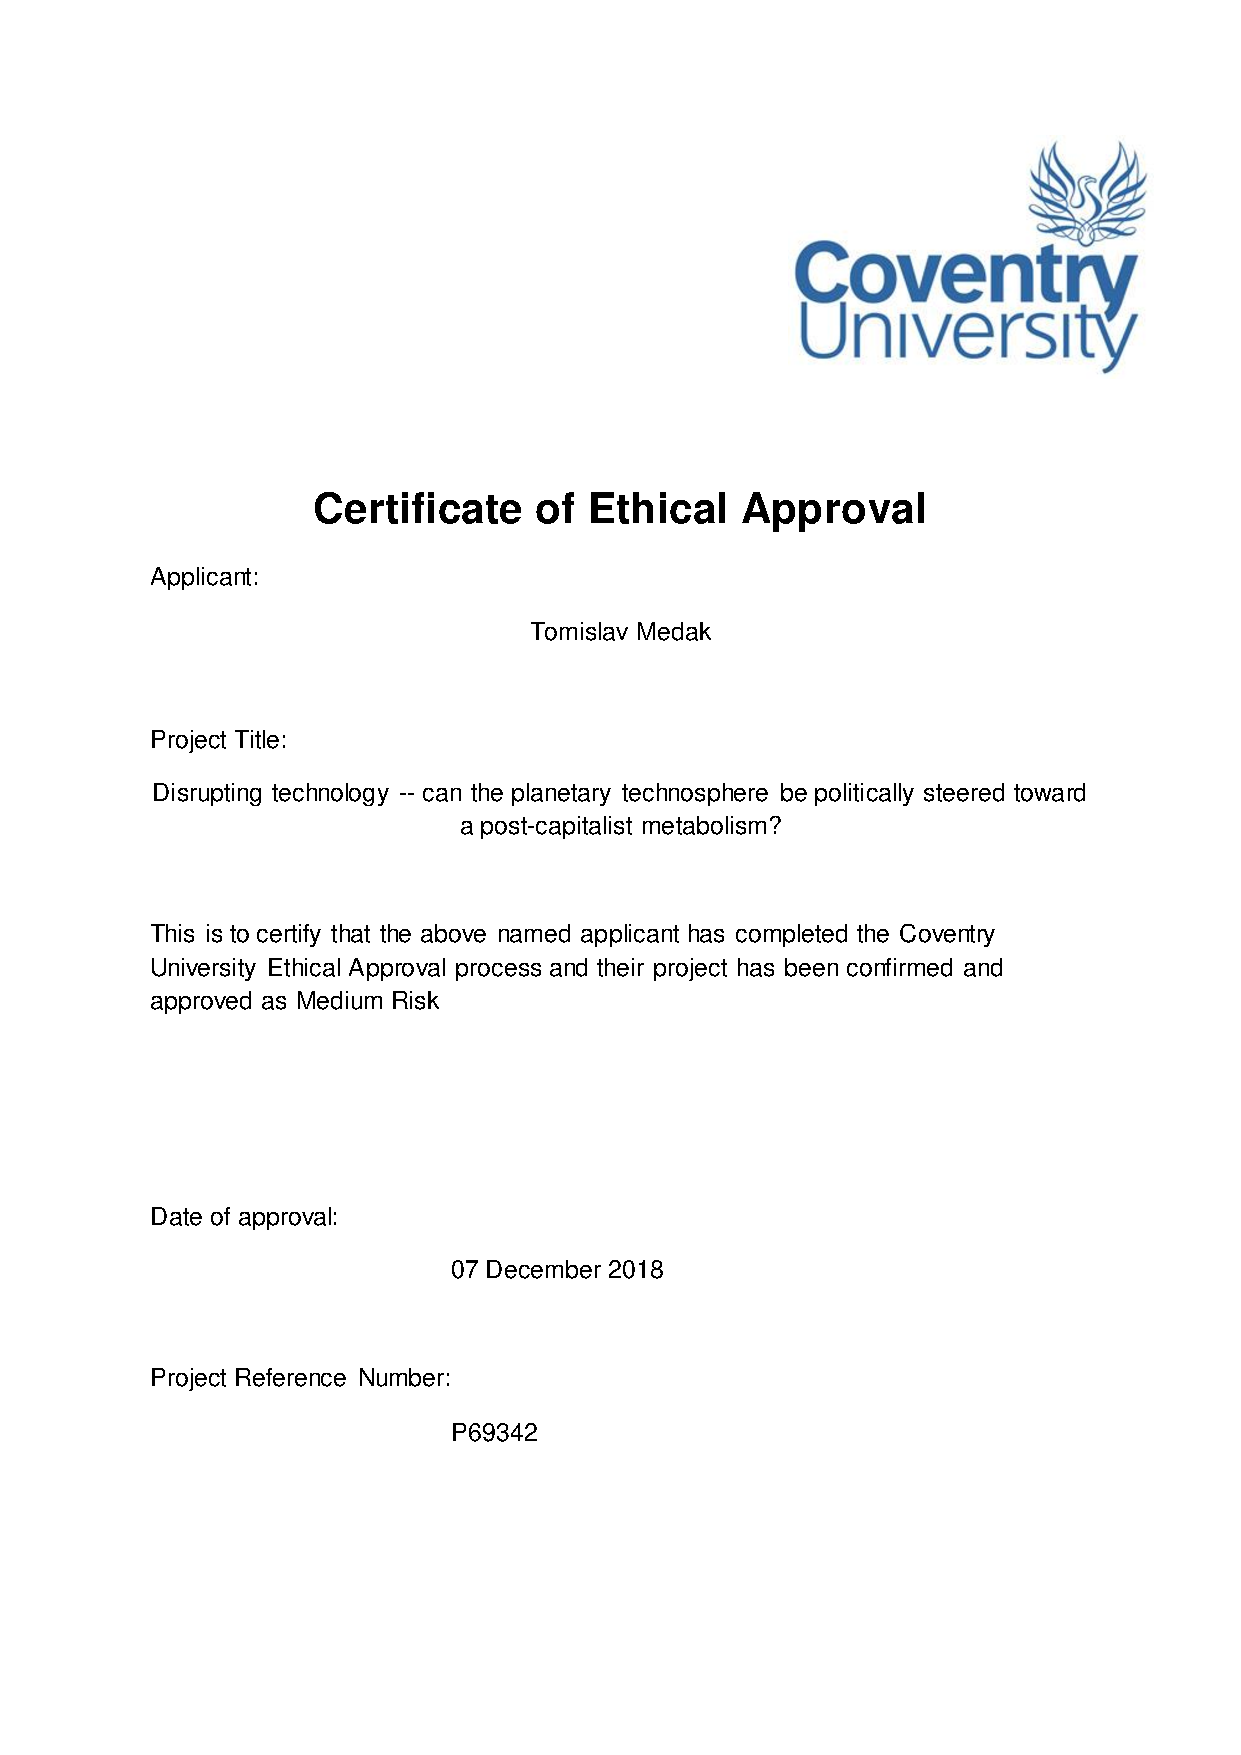
\includepdf[pages=-]{inserted-PDFs/ethics-certificate.pdf}

%%%%% CANDIDATE'S DECLARATION

\includepdf[pages=-]{inserted-PDFs/candidates-declaration.pdf}


%%%%% ABSTRACT SEPARATE
% This is used to create the separate, one-page abstract that you are required to hand into the Exam
% Schools.  You can comment it out to generate a PDF for printing or whatnot.

% JEM: Pages are roman numbered from here, though page numbers are invisible until ToC.  This is in
% keeping with most typesetting conventions.
\begin{romanpages}

% Title page is created here
\maketitle

%%%%% ABSTRACT


\renewcommand{\abstracttitle}{Abstract}
\begin{abstract}
	The dominant approach in (trans/sub)national governance of ecological crises, most notably climate change, is ecological modernisation. As a framing of collective action, ecological modernisation assumes that the structure of economic growth can be made sustainable by deploying market instruments to drive the sociotechnical transition away from the present fossil-fueled technological base. However, scientists are warning that such a market-driven technology-first approach, ensconced in the UNFCCC since at least the Kyoto Protocol, might not be comprehensive and rapid enough to prevent global warming beyond 2°C above the pre-industrial levels and thus a significant breakdown of ecosystems, rendering vulnerable indigenous, low-income, and working-class communities across the world.

 This thesis analyses how organisations that are operating in the ``middle ground,'' between the policymaking arena and their social constituencies, are seeking to disrupt the hegemony of technology-first policies, while at the same time proposing alternative pathways to transition away from the extractivist and capitalist social metabolism to a plurality of environmentally livable and socially just futures for all.

 Taking an iterative theory-building approach, the thesis first conceptualises the strategic agency of these social actors: against the historical trajectory of industrial-capitalist social metabolism; within the power-differentiated social structures of the capitalist state; and through the framing and distributive struggles sited between the climate action arena and the social field. By drawing on a set of complementary theories --- ecological Marxism, environmental humanities, science and technology studies, the critical theory of technology, strategic-relational approach, and institutional logics theory --- it proposes two analytical frameworks to indicate strategic openings for ``middle-ground'' organisations to impact sociotechnical and sociometabolic transitions.

 In a second step, the thesis provides two case studies contrasting two organisations and two environmentalisms: a degrowth-oriented Institute for Political Ecology, hailing from the periphery of European capitalism; and a green new deal-oriented industrial trade union Unite the Union, hailing from one of the centres of European capitalism. Drawing on interviews, analysis of documents, and joint research with the two organisations, it argues that they engage the governance terrain as epistemic actors and work with different social constituencies to instil distributive justice into climate action. These actors are disrupting the dominant market-driven technology-first approach and are thereby re-politicising and re-democratising the environmental governance. In a final step, the thesis analyses and speculates on the prospects of their counter-proposals in the present political and environmental conjuncture.
\end{abstract}



%%%%% DEDICATION
\begin{dedication}
  For my father
\end{dedication}

%%%%% ACKNOWLEDGEMENTS


\begin{acknowledgements}
 	When one decides to do a doctoral thesis in their forties, there have been many consorts along the way that deserve to be thanked. Far too many.

  While the research I conducted for this thesis was motivated by an ecological crisis and a sense of urgency that trascend any particular place, I understand my work primarily through the localised efforts of the collectives I am part of. The decision to undertake a PhD goes back to a commitment my collective at Multimedia Institute/MAMA in Zagreb took more than a decade ago. We decided to continue articulating, organising, and struggling for the alternatives to transform our post-socialist, monoethnic, peripheral capitalist society --- including through research. For this decision I want to thank that collective, foremost Petar Milat, Teodor Celakoski, and Marcell Mars. Marcell has been my closest collaborator over the last decade and has opened the institutional avenue for this research.

  Since the mid-2000s that collective has helped organise social and political forces --- the Right to the City movement in Zagreb and the municipalist green-left parties Zagreb je NAŠ! and Možemo! --- that have made the analysis in this research politically necessary. If this research will contribute to its avowed goal of steering the industrial-capitalist social metabolism toward just and sustainable futures, it will be through the work of people active in and around these forces and my involvement in them. I am indebted to them for their political engagement, constant encouragement of my research, and a shared commitment to organise and intervene politically.

  This thesis stands on the shoulders of the organisations that I have collaborated with: Institute for Political Ecology and Unite the Union. Their commitment to transforming the present environmentally unsustainable and socially unjust system has grounded and guided my research. I am grateful for the camaraderie of their present and past collaborators: Mladen Domazet, Vedran Horvat, Andro Rilović, Nikolina Rajković, Tina Tešija, Jim Mowatt, Colin Potter, and Joan Francis, whom I wish success in their future efforts. Their work will continue to be my lodestar.

  To my supervisors, Gary Hall and Janneke Adema I want to thank for accepting the challenge to mentor a thesis that was initially overambitious and then increasingly drifted further away from their expertise, as well as for constant prodding to find my own voice and to kick the habits of writing I have acquired throughout the last two decades of my activist work. The contribution to knowledge, the coherence of the structure, and the solidity of the argument are the fruit of their careful reading and their intellectual generosity.

  The chapters of this thesis, in various stages of completion, were read by my Coventry University colleagues Peter Conlin, Adrienne Evans, and Chris Maughan. Their comments contributed to shaping the argument and structure beyond the chapters they had read.

  On a more personal note, since I started my PhD in 2018, many friends have followed first hand the process and helped me navigate through the obstacles of migrant life. First among many, my co-conspirator Valeria Graziano, but also Maddalena Fragnito, Rebekka Kiesewetter, Kaja Marczewska, and Scott DeLahunta.

  When one decides to do a doctoral thesis in their forties in another country, the lives of one's closest get disrupted. For their unwavering support, encouragement, and patience, I owe everything to my partner Ivana Ivković and my mother Anka Medak. They have helped me through my moments of doubt.

  I dedicate this thesis to my late father, Ivan Medak, who has gone out of his way to help me never feel limited by the social circumstances of my disability and who has been absent from my life for over a quarter of a century. I regret not being able to share my concerns over the livable futures of others with him. It is a seed he has planted.

  \pagebreak

  \mbox{}
  \vfill

  Earlier versions of some of the materials in this thesis were published as ``Degrowth,'' a co-authored contribution to the \emph{Encyclopedia of the World's Biomes}; as ``Na ulicama Francuske povijest anticipira budućnost,''a reflection text on yellow vests published in \emph{Novi Plamen}, December 20, 2018; and as ``Fragilità, cura e azione politica,'' a reflection text written in March 2020 on the coronavirus and the planetary environmental crisis, included in the collected volume \emph{Dialoghi sulll pandemia: Crisi, riproduzione, lotte}, edited by Ecologia Politica Network, red star press, 2021. Some of the materials were self-published within the Pirate Care project (\url{https://syllabus.pirate.care}) and on my website (\url{https://tomislav.medak.click}).
\end{acknowledgements}



%%%%% MINI TABLES
% This lays the groundwork for per-chapter, mini tables of contents.  Comment the following line
% (and remove \minitoc from the chapter files) if you don't want this.  Un-comment either of the
% next two lines if you want a per-chapter list of figures or tables.
  \dominitoc % include a mini table of contents

% This aligns the bottom of the text of each page.  It generally makes things look better.
\flushbottom

% This is where the whole-document ToC appears:
\tableofcontents

\listoffigures
	\mtcaddchapter
  	% \mtcaddchapter is needed when adding a non-chapter (but chapter-like) entity to avoid confusing minitoc

% Uncomment to generate a list of tables:

%%%%% LIST OF ABBREVIATIONS
% This example includes a list of abbreviations.  Look at text/abbreviations.tex to see how that file is
% formatted.  The template can handle any kind of list though, so this might be a good place for a
% glossary, etc.

% The Roman pages, like the Roman Empire, must come to its inevitable close.
\end{romanpages}

%%%%% CHAPTERS
% Add or remove any chapters you'd like here, by file name (excluding '.tex'):
\flushbottom

% all your chapters and appendices will appear here
\hypertarget{introduction}{%
\chapter{Introduction}\label{introduction}}

\minitoc

\hypertarget{disrupting-technologies}{%
\section{Disrupting technologies}\label{disrupting-technologies}}

The title of this thesis contains an ambiguous phrase: ``disrupting technologies.'' Does the gerund mean to say technologies are causing a disruption or technologies are being disrupted?\footnote{For the purposes of this thesis, technology is understood as \emph{interlocking, formally organised material and symbolic systems that constitute and structure sociometabolic exchanges between human societies and non-human nature}. The thesis repeatedly resorts to a few foundational concepts: technology, the capitalist mode of production, social metabolism, planetary boundaries, and environmentalism. Their definitions are provided in Annex I.} The idea that technologies are disrupting the economic and social status quo has a time-honoured history from the days of the Industrial Revolution to the present. The \emph{Communist Manifesto} sang paeans to the bourgeoisie's revolutionising of the means of production, dislodging old industries and old class hierarchies, creating a universal condition of capitalist relations, proletarianisation, and ``interdependence of all nations,'' thus paving the way to a communist society (\protect\hyperlink{ref-marx_manifesto_1848}{Marx and Engels {[}1848{]} 2010, 488}). Evolutionary theories, rooted in the Gilded Age of the Second Industrial Revolution, contended more modestly that technologies transform institutions and, in turn, transform societies (\protect\hyperlink{ref-veblen_theory_1899}{Veblen {[}1899{]} 2007}). Or that innovations drive business cycles to destroy stagnant capital, unleashing new productive forces (\protect\hyperlink{ref-schumpeter_capitalism_1942}{Schumpeter {[}1942{]} 2013}). From there, the idea of technological disruption developed into a watchword of contemporary business theory, most notably enshrined in Clayton Christensen's concept of ``disruptive innovation'' (\protect\hyperlink{ref-christensen_innovators_1997}{1997}), foregrounding how emerging, smaller firms can use innovative business models and technologies to create new markets, push out the oligopolistic incumbents protecting their sunk investments, and thus disrupt the economic structure and the larger social order. Over the last couple of decades, as microcomputing and digitisation have unsettled traditional industries, technological disruption has thus become imperative for businesses and social institutions alike, leading the barons of industry such as Mark Zuckerberg to profess that they want ``to move fast and break things'' --- openly courting a ``destruction rhetoric'' (\protect\hyperlink{ref-zuboff_age_2019}{Zuboff 2019, 50--51}).\footnote{The exponential expansion of microcomputing and digital networks has come to shape the contemporary popular expectations of sociotechnical transitions. Digital technologies are perceived as maverick forces of the ``creative destruction'' of old oligopolies and bureaucratised institutions. Some of the transformations facilitated by digital technologies have indeed been unprecedented. Computerised control, coordination, and optimisation of geographically distributed processes have accelerated the integration of the post-1989 global free markets, the relocation of manufacturing to South East Asia, and the creation of global just-in-time supply chains. These transformations only pale in comparison to the changes in private and mass communication. These disruptions, however, have not come without significant political destabilisation and growing redistribution to the top, drawing an increasing public and regulatory scrutiny.} As a consequence, expectations that technologies can disrupt the impasses of status quo, that they are the most expedient way to tackle the hardest societal challenges, have thus come to dominate the contemporary social imaginary.

Environmental policies are no exception. The cornerstone tenet of the UN Framework Convention on Climate Change (UNFCC), ensconced in the Kyoto Protocol, is that climate protection should be achieved through ecological modernisation (\protect\hyperlink{ref-backstrand_climate_2016}{Bäckstrand and Lövbrand 2016}). Ecological modernisation assumes that, by using technologies and markets to replace the old fossil-fuelled technological base, economic growth can be harmonised with environmental sustainability. There is some merit to these expectations: pollution does happen through technologies. They are at least its material cause. However, many researchers indicate that --- given the state of green technologies development, the historical and present technological replacement rates, and the current investments into these technologies (\protect\hyperlink{ref-loftus_critical_2015}{Loftus et al. 2015}; \protect\hyperlink{ref-anderson_trouble_2016}{K. Anderson and Peters 2016}; \protect\hyperlink{ref-allwood_technology_2021}{Allwood 2021}; \protect\hyperlink{ref-hansen_november_2021}{Hansen, Sato, and Kharecha 2021}) --- such expectations underestimate the scale and the temporality of the challenge of limiting the global warming to the aspired 1.5 or 2°C above the pre-industrial levels.

These expectations thus might be unrealistic. The attained scale of the existing polluting technological infrastructures in energy generation, manufacturing, industrial agriculture, heating and cooling, which has been likened to a geological sphere --- a technosphere (\protect\hyperlink{ref-haff_technology_2014}{Haff 2014}), makes the rapid and disruptive replacement of fossil fuels much more challenging than were the changes in communication, coordination, and administration brought about by digital technologies. While significant advances have been made in energy generation, all other technological systems remain highly dependent on fossil fuels. Fossil fuels still account for around 85\% of the world's primary energy demand (\protect\hyperlink{ref-ren21_five_2021}{REN21 2021a}). Additionally, the temporal horizon for this colossal transition to a sustainable technological base is limited. As the IPCC warned in 2018, at the current rate of greenhouse gas emissions, by 2030 the world will have exhausted its carbon budget to remain within 50:50 chances of keeping the global warming down to 1.5°C (\protect\hyperlink{ref-ipcc_global_2018}{IPCC 2018a}). Contemporary industrial-capitalist metabolism, premised on the intensive extraction of matter and energy from nature, has been developed over centuries. Replacing it in a few short decades might not be achievable. Placing primacy on technologies in this rapid transition to sustainability might not yield timely results, implying that societies might need to consider other far-reaching transformations, including changes to their economic systems and their provisioning for social needs, to meet the goals of stabilising climate and other Earth's biophysical subsystems more easily. \emph{Thus, to reverse the expectations implied in the title, is it not the technology-first strategies that might need to be disrupted?}\footnote{Throughout this thesis I will use \emph{italicised text} to highlight definitions, insights, and conclusions that advance my argument.}

And indeed, both the Intergovernmental Panel on Climate Change (IPCC) and the Intergovernmental Science-Policy Platform on Biodiversity and Ecosystem Services (IPBES) have called for ``transformative changes across economic, social, political and technological factors'' (\protect\hyperlink{ref-ipbes_global_2019}{IPBES 2019}). While scientists thus demand transformative changes across different societal (sub)systems, policymakers stick to the changes to technology and energy systems, avoiding direct interventions into wasteful and unsustainable patterns of production and provision sustained by these technological and energy systems. Partly because social or political changes are more difficult to negotiate and enact than technological changes, both nationally and, in particular, internationally. But partly also because technologies are central to economic growth, develop from the capitalist centre, and redistribute social and environmental wealth to the centre (\protect\hyperlink{ref-hornborg_global_2016}{Hornborg 2016}). Technologies might be a material cause of pollution, but its efficient and final causes are economic, social, and political.

Policymakers' technological bias is only reaffirmed in the political imaginary by notions such as Anthropocene. The Anthropocene instils the idea that human ingenuity has caused this predicament and now that ingenuity has to solve it: to transform from a reckless planetary polluter to a responsible planetary steward. As degrowth scholar Stefania Barca (\protect\hyperlink{ref-barca_forces_2020}{2020}) has forcefully argued, such reasoning is an ideational extension of the aspiration for human mastery over nature. It ignores that the Earth's systems' stability has rested on the contributions of relations other than those of capitalist production: socially and environmentally reproductive relations fostered by subsistence farmers, land protectors, care-labourers, other species, and ecosystems that pre-date technological revolutions. Packing together a sense of human hubris and a sense of an impending catastrophe, notions such as Antrhopocenes thus occlude and foreclose class and other social antagonisms that inhere in climate crisis (\protect\hyperlink{ref-swyngedouw_apocalypse_2013}{Swyngedouw 2013}).

Facing these scalar, temporal, and ideational challenges, the centrality of markets and technologies in the transition to a purportedly sustainable future needs to be scrutinized and contested.

\hypertarget{thesis-at-a-glance}{%
\section{Thesis at a glance}\label{thesis-at-a-glance}}

The primary objective of this thesis is to investigate the proposals of alternative environmental action contesting that centrality and thus filling the gap between what science demands and what policy delivers. This thesis looks to proposals that might counteract a potential failure of the market-driven technology-first strategies to prevent a runaway global warming, but also to proposals that democratically ground environmental action in the lived reality of communities in a highly unequal world. The closing time window makes it urgent and necessary that the proponents of these alternatives shift the dominant framing of effective climate action: from ecological modernisation, aimed at harmonising economic growth with environmental sustainability, to framings that prioritise social wellbeing within the limits of a stabilised planetary ecology. This thesis responds to the urgency and the necessity of that frameshift.

To pursue that objective, I focus on two framings, their two proponents, and their exemplary agency. I do so to reflect the fact that social metabolisms\footnote{For a definition of ``social metabolism'' see Annex I.} encompass both \emph{the systems of production} and \emph{the systems of provision for social needs} and that they vary immensely between the affluent countries of the capitalist centre and the capitalist (semi)periphery. For this purpose, in the context of the European post-socialist semiperiphery, I investigate the activities of the Institute for Political Ecology (IPE), a research and educational organisation developing proposals for degrowth. Degrowth environmentalism offers a framing in which the limiting of economic growth in affluent societies, when accompanied by a redistribution of existing social wealth and an economy designed to provide the wellbeing for all, would lower the demand for material extraction and energy generation. This would ease the technological challenge of rapid decarbonisation and allow non-affluent societies to pursue their own development paths. The perspective from a post-socialist semiperiphery contributes a sense that a social transition to sufficiency might be politically feasible under conditions of large-scale redistribution and distributive justice.

Conversely, in the context of the European capitalist centre, I investigate the activities of the UK's largest industrial labour organisation, Unite the Union (Unite), whose environmental activities are aimed at developing proposals along the lines of a just transition and green new deal. The idea of a green new deal offers a framing in which the greening of the economy is fundamentally tied to making increasingly unequal economies more equitable and welfare provisions more comprehensive. To facilitate that coupled social and industrial transformation, such proposals are frequently premised on nationalising key polluting sectors such as energy and transport and socialising key welfare sectors such as healthcare, education, and housing. The perspective from the capitalist centre and its industrial base contributes a more ambivalent sense of the uncertainties of future transitions and sustainability.

The selection of these two actors as case studies has been motivated, however, by a desire to complicate the binaries through which their approaches are typically contrasted: working-class vs social-metabolism-oriented environmentalism, capitalist centre vs (semi)periphery, production vs social reproduction.\footnote{For a definition of ``environmentalism'' see Annex I.} By providing a pluriperspectival account of these organisations' strategic-operational contexts, my research aspires toward an understanding of the prospects of these two environmental positions in the present political conjuncture.

The research for this thesis has unfolded in two phases. In the first phase, I sought to ground the empirical research in historical, strategic, and political-epistemic analyses of the constraining and enabling factors such alternative framings and their proponents face. My inquiry drew on various disciplines and approaches --- including ecological Marxism, environmental history, science and technology studies, post-normal science, strategic-relational approach, and institutional logics theory --- in order to adequately conceptualise the current terrain of struggle over the sociometabolic transition and the strategic agency of ``middle-ground'' organisations such as IPE and Unite. Starting from that analytical framework as a propedeutic for empirical research, in the second phase, my research engaged the two organisations directly through fieldwork. My primary focus was on the organisation-field dynamic: how do IPE and Unite work to produce expertise and work with their social constituencies to affect the field of environmental action (rather than the individual-organisation dynamics shaping these entities from within). Once completed, the fieldwork and co-research with these actors then served to expand the initial theoretical conceptualisation and to speculatively assess the future prospects of their respective environmentalisms.

The methodology I have selected is aimed at building an applied theory of ideational and material struggles over sociotechnical and sociometabolic transition from within the present conjuncture and from the standpoint of these actors. It develops an interpretivist institutional analysis of how organisations such as IPE and Unite can contribute to shifting the framing of environmental action and steering it onto another pathway. My principal approaches were iterative theory-building and embedded case studies. Methods I have used in conducting these case studies, although transformed in their implementation by the intervening circumstances of the COVID-19 pandemic, included an analysis of the primary and secondary literature, participant observation, semi-structured interviews, and co-research, allowing for a pluriperspectival capture of the strategic, epistemic, and social agency of these organisations. Furthermore, I engaged the organisations in the spirit of militant research, seeking to directly support and extend their proposals and actions developed in opposition to the dominant ecological modernisation framing.

\hypertarget{positionality-of-research}{%
\section{Positionality of research}\label{positionality-of-research}}

Viewed in terms of my positionality as a researcher, the motivating factor behind this thesis is rooted in militancy and is collectively determined. The initial proposal for this research has developed from my experience of joint activist work with environmental groups and trade unions in Croatia over the last twenty years. In the early 2000s, the interests of the collectives I was part of were in technologies, politics, and the commons. Building on that work on digital commons, these collectives started to interrogate urban redevelopment processes that in the mid-2000s transformed formerly societal goods under Yugoslav socialism into new frontiers of enclosure and accumulation. As part of the Right to the City movement in Zagreb, we helped initiate a series of mass mobilisations between 2006-2015, which contested the privatisation of public land, national highways, and public services. Over the course of these mobilisations, Right to the City collaborated closely with Croatia's largest environmentalist organisation and Friends of the Earth affiliate, Green Action, and several public-sector trade unions (\protect\hyperlink{ref-MedakIndependentCulturalWork2017}{Medak 2017}).

Toward the end of that period my intellectual interests shifted toward researching the socioeconomic drivers of technological change. This led to my being asked on repeated occasions by our allied environmentalist organisation to present on the subject of technologies in relation to the planetary ecological crisis. In 2016 at the Green Academy summer school and at the International Degrowth Conference, both co-organised by IPE, I gave talks on ``Technologies for an Ecological Transition'' (\protect\hyperlink{ref-medak_technologies_2018}{Medak 2018}), presenting my research on the affordances and pitfalls that alternative technologies present for a transition to a post-growth metabolism, with a particular focus on what actors from the semiperiphery could do and should strive for. This was my first foray into the research interests that have led to this thesis. Since then I have become increasingly involved in environmental activism. This was the primary factor motivating me to better understand the strategic capacity that actors such as environmental groups and trade unions have in shaping the future direction of technological change while ensuring that that change can also lead to more sustainable and just socioecological arrangements than the present extractivist, growthist, and uneven capitalist development. While this thesis provides an appreciative account of the work of environmental groups and trade unions, it also wants to contribute to their collective analysis a theoretically-grounded and cautious reading of structural and conjunctural constraints and opportunities in contesting the status quo of environmental (in)action.

Furthermore, the work on this thesis has ramifications beyond research and environmental activism. Over the last five years, through my involvement with the municipalist green-left platform Zagreb je NAŠ! and the national green-left platform Možemo!, I have become a member of the working bodies of a political party that has recently, and unexpectedly, gained significant leverage on local and national environmental politics. In the 2020 national elections Možemo!-led coalition won five seats in the parliament, and in the 2021 municipal elections Zagreb je NAŠ! won the mayoral position, almost a majority in the city assembly, and majorities across most neighbourhood and district councils in the city of Zagreb. Currently, I am their programme coordinator and a member of the green transition working group. Three aspects of the research I have done for this thesis bear on that political work. Firstly, in a context of environmental policy dominated by a technology-first approach, frequently agnostic toward the social aspects of transition, my research highlights the primacy of social processes driving technological change and the diverging social outcomes resulting from different technological choices. Secondly, it suggests that rapid decarbonisation, ecosystem restoration, and other urgent measures to prevent further destabilisation of Earth's biophysical processes necessitate changes to how societies structure the provisioning for their members' needs. Thirdly and decisively, it indicates that such transformations need to be first experienced before they can gain popular acceptance and democratic legitimation. In that collective familiarisation with new, more sustainable and just modes of living, social actors such as environmental groups or labour organisations, operating in what I have called the ``middle ground,'' where they shape quotidian practices and common senses --- play a catalysing role. The implication is that a pivotal part of transformative environmental politics should be to strengthen the strategic agency of these actors and the practices they are developing in their particular social contexts.

\hypertarget{research-objectives-and-questions}{%
\section{Research objectives and questions}\label{research-objectives-and-questions}}

While the initial motivation for this research might be activist and political, the invocation of ``political steering'' in the subtitle of this thesis refers rather to a larger process of re-politicisation. The subtitle --- can the planetary technosphere be steered politically toward a post-capitalist social metabolism? --- aims at reconsidering how the dominant forms of environmental action instituted by (trans/sub)national governance can be effectively contested, and how they can be reoriented from a market, bureaucratic, and technological logic to a democratic-redistributive one. \textbf{The overall goal} is to develop understandings of the strategic capacity of organisations such as environmental groups and trade unions to do so --- and to do so by shifting the environmental action away from the market-driven technology-first approach toward fostering more sustainable and just social metabolisms.

However, directly researching these organisations, with whom I also share activist and political causes, could easily lead to a potentially voluntarist assessment, if their strategic capacity to steer toward a post-capitalist social metabolism were not analysed within the constraining and enabling factors imposed on them by the present social metabolism and the structures of the capitalist economy and the state. The research, therefore, pursues the overall goal through three related research objectives.

\textbf{The first objective} is to provide an \emph{historical analysis} of how the fossil-fuelled industrial-capitalist social metabolism emerged, evolved, and consolidated. Specifically, it is to analyse \emph{what processes have driven the transitions to that presently dominant sociometabolic regime, and, in turn, what impediments does that regime impose on achieving sustainable and just social metabolisms in the future?} The technological, energetic, material, and socioeconomic lock-ins, inherent to that regime, are already an immense obstacle for a technology-first transition aimed toward greening the existing technological infrastructures, let alone for alternative proposals that might want to reduce energetic, material, and economic impacts. Therefore, understanding the scale, the social processes that have led to that scale, and the arrangements that sustain that scale is necessary to situate the strategic agency within the material and social complexities of transition from one social metabolism to another.

\textbf{The second objective} is to elaborate elements of a \emph{theory of agency in structure} and \emph{political epistemic middle ground} delimiting the strategic capacity of various actors within political, institutional, and social processes shaping and driving sociotechnical and sociometabolic transitions. This conceptualisation devises a framework to comprehend specifically the agency of environmental groups and trade unions, by asking the questions: \emph{Can social actors that are neither governments, corporations, or scientific bodies be catalysts of sociotechnical and sociometabolic change? Can they envision such transitions, produce the necessary expertise, and shift their dominant framings in significant ways? Can they engage their social constituencies to ground environmental action in their lived experience and conditions of inequality impacted by environmental policies?} This theoretical conceptualisation draws out the strategic opportunities afforded to the ``middle-ground'' actors by the ecological imperatives of social development that are weaking the capitalist economy's determining power over transition and open avenues for framing struggles that can contest the adequacy of technology-first strategies.

While the first two objectives are aimed at a more general inquiry of what are the enabling and constraining factors to re-politicise the environmental action, \textbf{the third objective} is to provide an account of \emph{how organisations attempt to do this concretely}. That is, the objective is to engage an environmental group in Croatia and an industrial trade union in the UK, analysing and contributing to their strategies and alternative proposals in contesting the dominant market-driven technology-first approach. The fieldwork with these organisations considers \emph{how do such actors concretely envision and act to shift the framing of environmental action toward a post-capitalist social metabolism? How do they ground these proposals in the practices of social constituencies they work with? And what are the future prospects of their proposals?}

How these research questions have evolved is discussed in more detail in the next chapter on methodology. Historical, strategic and epistemic analyses corresponding to objectives 1 and 2 are provided in chapters 3, 4 and 5, whereas the engagement with the IPE and Unite corresponding to objective 3 is provided in chapters 6 and 7. I will return to explain this structure in the thesis outline below.

\hypertarget{gap-in-the-existing-research-and-contribution-to-knowledge}{%
\section{Gap in the existing research and contribution to knowledge}\label{gap-in-the-existing-research-and-contribution-to-knowledge}}

While I indicated earlier that this research is pragmatically motivated, seeking to contribute with its analysis to collective activist efforts, the question remains: where is it situated and what does it contribute in terms of scholarship?

The starting point for my inquiry lies at the intersection of theories investigating technological change, collective action, and ecology. It takes a synthetic approach, drawing on diverse bodies of research on these subjects, \emph{to construct a comprehensive perspective on the problem of how large-scale transformation of the capitalist social metabolism can be instigated by a situated strategic agency of social actors}. This comprehensive perspective integrates both the present conjuncture and the standpoint of the particular organisations I engage with.

Concretely, my inquiry is situated within the research paradigm of sociometabolic transitions that has now been three decades in the making, most notably in environmental history (\protect\hyperlink{ref-cronon_natures_1992}{Cronon 1992}; \protect\hyperlink{ref-pomeranz_great_2000}{Pomeranz 2000}; \protect\hyperlink{ref-barca_energy_2011}{Barca 2011}), environmental humanities (\protect\hyperlink{ref-chakrabarty_climate_2009}{Chakrabarty 2009}; \protect\hyperlink{ref-ghosh_great_2016}{Ghosh 2016}), ecofeminism (\protect\hyperlink{ref-merchant_theoretical_1987}{Merchant 1987}; \protect\hyperlink{ref-plumwood_environmental_2005}{Plumwood 2005}; \protect\hyperlink{ref-haraway_staying_2016}{Haraway 2016}; \protect\hyperlink{ref-tsing_mushroom_2015}{Tsing 2015}; \protect\hyperlink{ref-barca_forces_2020}{Barca 2020}), ecological Marxism (\protect\hyperlink{ref-burkett_metabolism_2006}{Burkett and Foster 2006}; \protect\hyperlink{ref-foster_ecological_2011}{Foster, Clark, and York 2011}; \protect\hyperlink{ref-huber_lifeblood_2013}{M. T. Huber 2013}), and social ecology (\protect\hyperlink{ref-sieferle_subterranean_2001}{Sieferle 2001}; \protect\hyperlink{ref-krausmann_global_2008}{Krausmann et al. 2008}; \protect\hyperlink{ref-fischer-kowalski_analyzing_2011}{Fischer-Kowalski 2011}). This literature is discussed, commented and built upon in my historical account of the rise of industrial-capitalist social metabolism and the dominance of fossil fuels.

Furthermore, it is situated within subdisciplines in technology studies theorising the determining role of technologies in social change and the determining role of social relations on technological change --- including the social construction and social shaping of technology (\protect\hyperlink{ref-schwartz_cowan_more_1985}{Schwartz Cowan 1985}; \protect\hyperlink{ref-hughes_networks_1993}{Hughes 1993}; \protect\hyperlink{ref-mackenzie_knowing_1998}{MacKenzie 1998}; \protect\hyperlink{ref-mackenzie_social_1999}{MacKenzie and Wajcman 1999}), science and technology studies (\protect\hyperlink{ref-callon_techno-economic_1990}{Callon 1990}; \protect\hyperlink{ref-latour_we_1993}{Latour 1993a}; \protect\hyperlink{ref-law_aircraft_2002}{Law 2002}; \protect\hyperlink{ref-sismondo_introduction_2009}{Sismondo 2009}), and Marxian critique of technology (\protect\hyperlink{ref-slater_outlines_1980}{Slater 1980}; \protect\hyperlink{ref-smith_does_1994}{Smith and Marx 1994}; \protect\hyperlink{ref-davis_cutting_1998}{Davis, Hirschl, and Stack 1998}; \protect\hyperlink{ref-feenberg_transforming_2002}{Feenberg 2002}; \protect\hyperlink{ref-noble_forces_2011}{Noble 2011}; \protect\hyperlink{ref-dyer-witheford_cyber-proletariat_2015}{Dyer-Witheford 2015}). I consider these theories in combination with theories analysing the interactions of social actors, institutional orders, and social structures within the capitalist state, specifically structuration theories (\protect\hyperlink{ref-giddens_constitution_1984}{Giddens 1984}; \protect\hyperlink{ref-sewell_theory_1992}{Sewell 1992}), the strategic-relational approach (\protect\hyperlink{ref-jessop_state_2008}{Jessop 2008}), and institutional logics approach (\protect\hyperlink{ref-friedland_bringing_1991}{Friedland and Alford 1991}; \protect\hyperlink{ref-thornton_institutional_2008}{Thornton and Ocasio 2008}). By combining sometimes complementary and sometimes contrasting theories of agency, technology, and structure in novel ways, I build my own analytical frameworks that are specific to the ``middle ground'' organisations I am researching and to the conjuncture in which they have to act.

Finally, it is situated in a growing body of research, much of it participatory or ethnographic, that has been carried out on the role of activism and trade unionism in the global environmental arena (to mention some of the most notable: \protect\hyperlink{ref-reitan_climate_2012}{Reitan and Gibson 2012}; \protect\hyperlink{ref-klein_this_2014}{Klein 2014}; \protect\hyperlink{ref-hampton_workers_2015}{Hampton 2015}; \protect\hyperlink{ref-barca_working-class_2018}{Barca and Leonardi 2018}; \protect\hyperlink{ref-malm_how_2021}{Malm 2021}; \protect\hyperlink{ref-riofrancos_resource_2020}{Riofrancos 2020}). However, there is limited research on the shaping capacity of environmental activism and trade unionism on the sustainability transition from both technological and strategic perspectives (\protect\hyperlink{ref-rathzel_trade_2013}{Räthzel and Uzzell 2013}; \protect\hyperlink{ref-backstrand_climate_2016}{Bäckstrand and Lövbrand 2016}; \protect\hyperlink{ref-dawson_peoples_2020}{Dawson 2020}). My thesis sits in this gap and seeks to contribute original theorising of that strategic capacity in the present conjuncture.

The thesis contributes to that scholarship in four principal respects. Firstly, by combining these various strands of theorising in novel ways, \emph{I devise two related analytical frameworks, one of the larger structural terrain of agency in sociotechnical transition and another of the strategic terrain for the ``middle-ground'' organisations to shift the framing of that transition}. These models add to the understanding of what are the structural factors that limit and enable actors that are neither governments, corporations, nor scientific bodies to disrupt the dominant forms of environmental (in)action and transform these forms from the bottom-up. There is an urgency and necessity to analyse their strategic capacity in the present conjuncture, which is defined, paradoxically, by the increasingly evident faltering of the (trans/sub)national governance process to limit the global warming to 1.5°C or 2°C above industrial levels, and, at the same time, the electoral defeats of the proponents of democratic and redistributive environmental politics of green new deal in the US and the UK. The theory-building I undertake in this thesis is an effort to draw out elements on which to debate strategic openings in that seeming impasse.

Secondly, \emph{I offer an original perspective on how these actors' positionality allows them to work with their social constituencies to ground environmental action in distributive conflicts and the lived reality of these constituencies}. While climate change policy is framed in terms of long-term collective action of global society that seemingly does not have an immediate impact within societies, the recent scholarship indicates that the effective national climate action hinges on distributive conflicts between the polluters and the rest (\protect\hyperlink{ref-aklin_prisoners_2020}{Aklin and Mildenberger 2020}; \protect\hyperlink{ref-mildenberger_carbon_2020}{Mildenberger 2020}). The central question is who bears the existential cost. The answer is that the masses are made to carry these costs either through climate-driven natural disasters or the rising carbon prices of energy and essential goods. I extend this focus on distributive conflicts by elaborating that the ``middle-ground'' organisations are in a unique position to make those conflicts manifest and ground their work in the socially unequal and environmentally destabilised conditions affecting the contexts from which they operate. They can do so by working with the communities to translate the alternative proposals they develop into their lived reality and to translate their lived reality into their alternative proposals --- and from there further into the framing struggles pursued on the institutional terrain of (trans/sub)national climate governance. From the engagement with these organisations and the evidence I bring together of the epistemic, educational and organising efforts they are developing with their constituencies, I contend they can contribute to shifting the environmental action from a market-centred top-down logic to a democratic-redistributive bottom-up logic.

Thirdly, \emph{I contribute to the understanding of why both the existing technological infrastructures and the ongoing sociotechnical transition are susceptible to contestations that intervene locally to affect significant shifts in the larger political terrain}. I argue that the blockade, but equally mass organising and framing struggles around and against particular technological infrastructures and particular sociotechnical changes matter to the re-politicisation. Of particular interest are under-researched parallels between Big Tech and Green Tech, at a moment when Big Tech companies, characterised by a resistance to unionisation, are increasingly moving into and setting the blueprint for the Green Tech industries. I outline some of the valuable lessons that can be drawn from contestations against Big Tech for working-class environmentalism.

Finally and relatedly, I argue that for reasons of accumulated pollution and destabilisation of Earth's biophysical processes, a condition that Herman Daly has qualified as a ``full world'' (\protect\hyperlink{ref-daly_economics_2005}{Daly 2005}), the future is not an open horizon where all transition pathways are equally possible and adequate, as the seeming flexibility of global policies and nationally determined contributions might suggest. Through my analysis I add to the understanding of why alternatives to ecological modernisation are necessary and how they can be adequate --- by proposing strategies prioritising equitable wellbeing and environmental stability over a continued economic growth. \emph{I will contend that achieving environmentally livable and socially just futures in a destabilised planetary ecology requires both careful and urgent experimentation with alternative pathways, of which technological change is only one aspect among the many-sided and far-reaching economic, political, and social transformations}. While that might be evident from the degrowth perspective, it is less so from a trade-union perspective. But I propose why that might need to change. Therefore, I provide a speculative analysis of some of the proposals and alliances that the social-movement and the working-class environmentalisms can develop in the present conjuncture to again shift the terrain of struggle over environmentally safe and socially just futures.

\hypertarget{thesis-outline}{%
\section{Thesis outline}\label{thesis-outline}}

The next chapater, \textbf{chapter 2} outlines my methodology. It expands on the positionality and objectives discussed in this Introduction to elaborate how the stepwise development of research objectives and analytical framework served to select the two organisations for my case studies and prepare the fieldwork. And, in turn, how my interpretivist analysis of the agency of those two organisations worked back to inform a theory of sociometabolic transformation in the focus of this thesis. My principal methodological approaches were iterative theory-building and embedded case-study research. While doing fieldwork, I have engaged the organisations in the spirit of militant research, attempting to directly support and amplify their counterproposals to the hegemonic framing of ecological modernisation. The combination of these approaches was needed to situate the first-hand account of their agency gained through fieldwork within the structural analysis of technological, economic, and institutional factors that constraint and enable that agency, while allowing the militant motivation that has led to this research to extend into an assessment of what prospects their work might have in the future.

The methodology discussion segues into three chapters in which I develop my analytical frameworks from historical, strategic, and political-epistemic discussions. Throughout these chapters, agency aimed at sociometabolic transformation is analysed against the constraining and enabling factors of technology and the capitalist state.

\textbf{Chapter 3} harks back to a history of systemic, technological, and energy transitions from the 16th to the late 20th century that have led to the presently dominant fossil-fuelled industrial-capitalist social metabolism. It retraces entwined transitions from feudalism to capitalism, from renewable energy to first coal and then oil, from agricultural steady-state to globalised industrial growth, from the conservation of energy to inefficient large-scale energy systems, and from the early colonial capitalism to neo-imperial unequal ecological exchange. The central question I explore in this genealogy is whether these historical transitions were driven by technological advances or social antagonisms, indicating that social antagonisms and distributive conflicts have been key factors in the past transitions. The chapter's objective is to provide an account of the challenge that the presently dominant social metabolism sets before any future transition.

\textbf{Chapter 4} parallels that genealogy with a theoretical analysis of strategic agency in the structure of the present green transition. Discussing technological determinism, agency in stucture, and a critical theory of technology, I propose a framework to analyse agency in and against the social structures of the state and the capitalist economy. The framework indicates openings for actors other than corporations, technologists or governments to disrupt and change the course of sociotechnical and sociometabolic change. However, the lock-ins of fossil-fuelled technologies and the asymmetries of power result in significantly different capacities of social actors to effectively impact these transitions. To bring the chapter to a close, I argue that despite these asymmetries, the dependence of technological systems on regulatory arrangements and energy infrastructures makes them susceptible to direct political contestation, thus producing an avenue for non-linear transformations through three vectors of disruptive agency: blockade, organising and framing struggles.

While chapter 4 concludes with a reflection on the brittleness of technological infrastructures to the acts of blockade, \textbf{chapter 5} focuses on the other two vectors of disruption: framing struggles and organising. I propose a framework to analyse the ``middle ground'' of agency between the (trans/sub)national climate governance and social constituencies. The framework addresses the positionality of environmental groups and trade unions within the broader context of knowledge production and distributive conflicts in climate action. These organisations, although neither scientific institutions nor policymaking bodies, do engage in research activities and produce their own expertise to translate environmental science into the lived reality of their constituencies --- and vice-versa. To elaborate how the epistemic politics of such organisations can be reconciled with the objectivist principles of science, I analyse their work through the lens of feminist standpoint epistemology and the ``post-normal science'' necessitated by the urgency of the crisis. Finally, I contextualise their work on distributive conflicts within the broader climate change politics, asserting that the science-based climate action is rooted in the post-WWII liberal international order but is, at the same time, subverted by the economic neoliberalisation and the inequalities this order has given rise to. The groundedness in ideational and material interests of their social constituencies thus makes these actors into potential proponents of a pro-environmental transformation from below.

The three chapters focusing on theoretical conceptualisation segue into two case study chapters that draw on my fieldwork with the IPE and Unite. Both chapters include three macro-segments: a discussion of particular environmentalism, an analysis of the organisation and my engagement with the organisation, and a speculative exploration of the limitations and opportunities their form of environmentalism brings to the present conjuncture.

The first of the two, \textbf{chapter 6}, developed during my fieldwork with the IPE in 2019, starts by detailing the emergence of degrowth as a social-metabolism-oriented environmentalism. Degrowth coalesced in parallel into a global movement and a research project, developing proposals, theoretical and practical, on how to transform the destructive sociometabolic patterns of affluent societies by lowering the throughput of energy and matter, redistributing social wealth, and allowing a pluriverse of material and epistemic routes for societies outside of capitalism. From this general outline of degrowth environmentalism, the chapter moves on to the actions and positions of IPE. My principal engagement with the organisation was the participation in the development of a Degrowth Doughnut aimed at overcoming the opposition between nature and society and at providing a tool for democratic degrowth within different social metabolic units. The chapter concludes with a reflection on how degrowth is proposing a real-utopian horizon of sociometabolic transformation built on prefigurative practices, an approach taking the ``full world'' of destabilised planetary boundaries as truly limiting, and developing policies, practices, and tools to transition societies toward a good life within planetary boundaries for all.

The second case study, the basis for \textbf{chapter 7}, was initiated in late 2019 and was unexpectedly disrupted by the COVID-19 pandemic. Here I first outline the elements of working-class environmentalism, conceptualising the separation of internal from external nature within capitalism, as well as the various forms of the environmental vulnerability of the working class. From there, I analyse the strategic agency of the working class within the economic and environmental domain, arguing that organised labour developed forms of power from below that have significantly disrupted the direction of social development to create more democratic and environmentally safer societies. My analysis of Unite's environmental strategy is situated in this history, outlining its ambivalent positioning that includes both transformative components of green industrialisation and conservative components of support for polluting industries. The threat of the working class losing once again in the next transition (as it did in the UK's transition from coal) calls for a just transition that will provide security and jobs for workers and their communities as the fossil economy is phased out. The chapter concludes with a discussion of the waning political fortunes of the green new deal proponents who have argued that addressing social inequalities is a necessary prerequisite for climate action. I contend that given the labour movement's fragmentation, resulting from technological change, the onus is on the proponents of other environmentalisms to support the unionisation and help trade unionism again gain ground to advocate for more radical and community-oriented environmental proposals in return.

In the concluding chapter, \textbf{chapter 8}, I return to my initial research questions to argue how the take-aways from the two case study chapters, as well as from the historical, strategic and political-epistemic inquiries in earlier chapters, combine in novel ways to contribute to knowledge of the ecological agency of the ``disruptors'' of the market and technology approach. The conclusion suggests further avenues of research, particularly indicating the significance of ``middle-ground'' actors as the world moves from the expectations of climate change mitigation to the realities of climate change adaptation.

\hypertarget{methodology}{%
\chapter{Methodology}\label{methodology}}

\minitoc

\hypertarget{introduction-combining-research-approaches}{%
\section{Introduction: combining research approaches}\label{introduction-combining-research-approaches}}

The overall aim of the research for this thesis was to contribute to the understanding of whether the planetary technosphere can be politically steered toward a post-capitalist metabolism. I did so by looking to those organisations within capitalist societies that are neither governments, corporations, nor scientific bodies yet command some strategic capacity. By using environmental expertise, organising social constituencies, and developing practices and experiences of ecological transformation with them, they can disrupt the hegemonic framing of ecological modernisation that dominates in environmental politics. They have the capacity to push the collective action of societies into alternative directions, directions that do not rely primarily on technologies and markets but propose far-reaching economic, social, and political transformations to achieve socially just and environmentally safe futures for all.

The principal methodological approaches I used in conceptualising and analysing that strategic capacity were \textbf{iterative theory-building} and \textbf{embedded case studies}. These two approaches are complementary. The two case studies looked at the positions and actions of IPE and Unite and have focused my research on the substantive proposals of transformation they are advocating. However, looking only at agency from their perspective, a perspective I largely share, carried a methodological risk of leading to a voluntaristic assessment --- one that would affirm their claims of transformative agency without bracketing it from a structural perspective. Therefore, I have bracketed their agency within an analysis of the constraining and enabling factors of the presently dominant industrial-capitalist social metabolism, the structures of the capitalist state, and the sustainability transition they need to undergo. Developing those analytical frameworks prior to my fieldwork thus enabled me to theorise the strategic agency of the ``middle-ground'' social actors in more general terms.

Case studies were done through fieldwork. While conducting fieldwork, I have sought to engage IPE and Unite in the spirit of \textbf{militant research}, attempting to directly support and amplify their counterproposals to the hegemonic ecological modernisation framing. This orientation toward the causes I share with the organisations primarily took the form of my participation in their research and expertise-building activities --- through writing, dialogue, and organising work. Building on the direct engagement with the IPE and Unite, in the last step I have \textbf{speculatively reflected} on the challenges and opportunities their form of environmentalism, strategic agency, and interventions offer for the transformation of the fossil-fuelled industrial-capitalist social metabolism. These challenges and opportunities I analysed from the present conjuncture of climate action defined by the failing (trans/sub)national climate governance with its technology-first strategies and the parallel political defeats of the green new deal proponents.

The combination of these approaches --- iterative theory-building, case studies, militant research, and speculative reflection --- allowed my research to:

\begin{enumerate}
\def\labelenumi{\alph{enumi})}
\item
  situate the first-hand accounts of strategic agency within technological, economic, and institutional factors that constraint and enable that agency;
\item
  extend the activist experience that initially motivated this research into an assessment of the future prospects of the proposals of these organisations;
\item
  navigate closeness and critical distance in supporting and analysing their work.
\end{enumerate}

On that last point, the closeness in this research is also a reflection of the fact that it seeks to contribute to what it analyses --- challenge to the hegemony of the technology-first approach. My research responds to the warnings of scientists that the already unfolding green technology transition, barring larger economic, political, and social transformations, might be insufficient to prevent a significant climate change and destabilisation of the biosphere. These warnings make interventions into the hegemony of the technology-first approach to steer environmental action into another direction necessary and urgent. For reasons of that necessity and urgency my research could not take a distanced view of the two organisations and the causes they advocate. However, analysing structurally and conjuncturally the present and future challenges they face could not be done only by directly engaging these organisations. Thus, to arrive at an adequate problem-setting of their strategic agency in the context of the technological, economic, and governance structures underlying the industrial-capitalist social metabolism required an indirect and iterative approach.

Over the following sections, I will detail the research process as it worked back and forth between the problem setting and my engagement with the two organisations to develop and refine the preliminary objectives, the fieldwork objectives, and the positionality of militant research. The final section is reserved for outlining how my research process has built trust with the organisations I engaged.

\begin{figure}
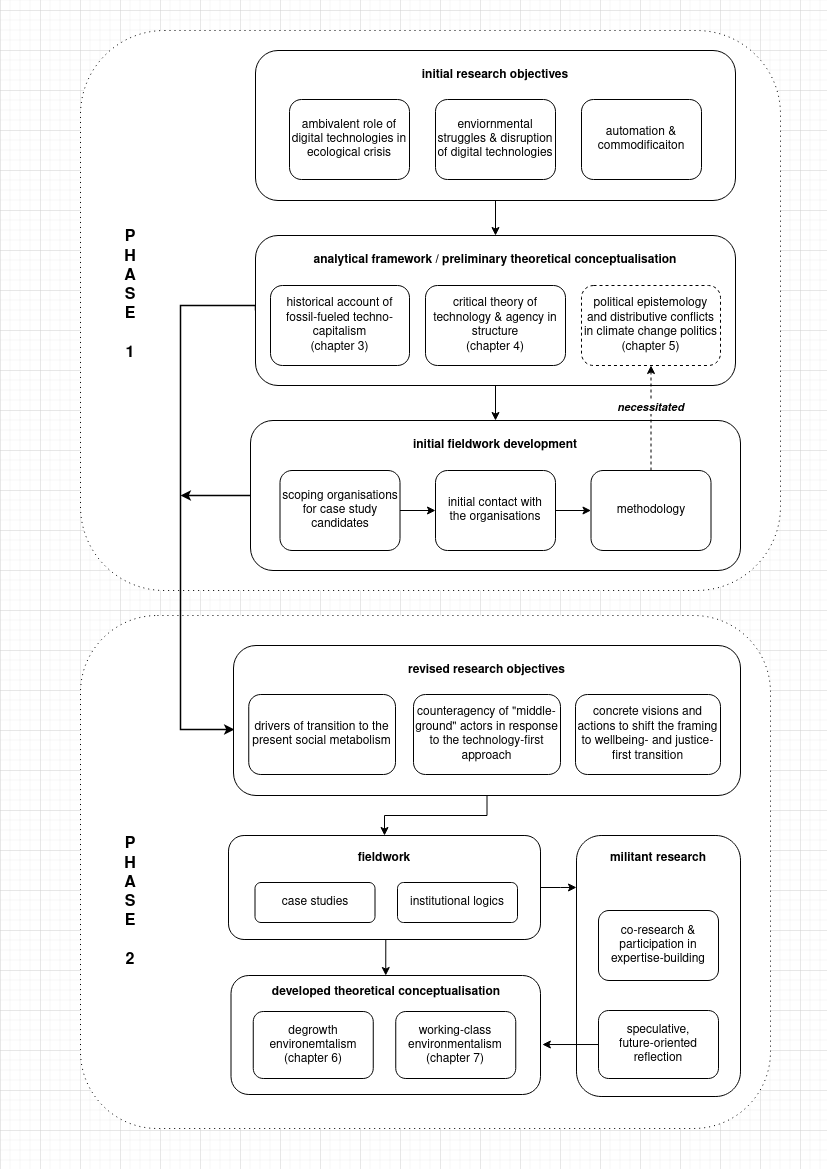
\includegraphics[width=1\linewidth]{./figures/methodology_diagram} \caption[Methodology overview]{Schema of iterative theory-building and methodological approaches in this thesis.}\label{fig:unnamed-chunk-1}
\end{figure}

\hypertarget{iterative-theory-building}{%
\section{Iterative theory-building}\label{iterative-theory-building}}

The back-and-forth in this research is based on the principles of iterative theory-building. In an iterative theory-building process, a preliminary theoretical conceptualisation and the initial cycle of empirical data gathering are used to reassess, redefine, and refine the research questions, analytical framework, and research strategies that are then taken into the next cycle of empirical research. Going back and forth between theory and empirical research, the process develops a new theory. According to the organisation researcher Kerssens-van Drongelen, iterative theory-building has the following two characteristics:

\begin{quote}
\begin{itemize}
\item
  new theory is built during various research cycles, allowing for a (conscious) change in the research question if empirical material already gathered requires this; and
\item
  research strategies, data collection and analysis methods and tactics are selected based on the (changing) type of research questions and process phases. This often results in a combination of research strategies within one research project. (\protect\hyperlink{ref-kerssens-van_drongelen_iterative_2001}{Kerssens-van Drongelen 2001, 510--11})
\end{itemize}
\end{quote}

Such methodology is similar to the original inductive grounded theory (\protect\hyperlink{ref-glaser_discovery_2017}{Glaser and Strauss 2017}), but greater importance is placed on the process of cycling back and forth between theorising and evidence-gathering (\protect\hyperlink{ref-orton_inductive_1997}{Orton 1997}). This back and forth is particularly suited for the development of new theory from first-hand, ethnographic accounts of a small sample of cases, as is the case in this thesis. As this thesis is building a theory of ``middle-ground'' social agency to shift the field of environmental action relying on an engagement with only two organisations, iterative theory-building was selected for that reason. As can be seen in \emph{Figure 2.1}, the theory-building proceeded in two phases. In the first phase, the formulation of the historical, strategic and political-epistemic analytical framework, the selection of case study organisations, and the initial engagement with the primary and secondary publications documenting their work were used to revise the initial research objectives and recalibrate the analytical framing. In the second phase, during and after the completion of the fieldwork, the research resulted in a new theory that includes first-hand accounts of the organisations I engaged with in the fieldwork, as well as the future-oriented speculative reflections on the prospect of their strategies moving ahead.

Concretely, in the initial stages of research development, my theoretical conceptualisation focused on \emph{digital technologies} and their ambivalent role in both accelerating ecological crisis and enabling agency and expertise that could overturn that acceleration. As I stated in my PhD proposal, the overall aim was:

\begin{quote}
First, \ldots to theorise how digital technologies are helping drive the acceleration of global material and energy flows that is the hallmark of the Capitalocene. Second, \ldots{} to empirically examine how they, at the same time, open up space for the collective agency of social movements, communities of expertise and interest groups --- allowing them to affirmatively disrupt and steer technological change toward a more equitable and sustainable post-capitalist social metabolism.
\end{quote}

The research objectives derived from this aim were to hammer out, drawing on a variety of theoretical approaches, an analytical framework and apply it empirically on: ``struggles around 1) environmental change and 2) automation of production in the context of 3) commodification of knowledge that shapes the availability of data, metrics and scientific knowledge.''

As I began to engage with the existing literature to hammer out that analytical framework and to establish communication with the organisations I intended to conduct my research with, I have decided to shift the focus of my conceptualisation away from the ambivalent role of digital technologies \emph{toward technologies and energy systems that are more fundamental to industrial-capitalist social metabolism}. The reason for this shift was that digital technologies are indeed the globally leading technological sector in terms of market valuations, investments in R\&D, and the coordination of global economic flows. However, they are entangled with other more polluting and older sociotechnical infrastructures that are inert to transformation. The underlying energy and production systems typically have greater footprints and are pivotal for manufacture, food production, transport, heating and cooling, construction, and warfare. The role of these underlying systems thus merited greater attention than digital technologies to analyse the industrial-capitalist social metabolism.

\hypertarget{reformulating-research-objectives}{%
\section{Reformulating research objectives}\label{reformulating-research-objectives}}

This shift resulted in a reformulation of my \textbf{first initial research objective}, with which I now aimed at providing an analysis of how we have arrived at the present social metabolism and the challenge it sets for future transitions in terms of path dependence, structural impediments, and global governance structures. Accordingly, the initial part of the theoretical conceptualisation, which I develop in chapter 3, proposes a historical frame of analysis, pointing to the transitional processes in the origins and subsequent development of fossil capitalism. The argument I make in chapter 3 denaturalises the notion that the presently dominant industrial-capitalist social metabolism has simply evolved through technological progress. I resort to \emph{environmental history}, \emph{ecological Marxism}, and \emph{sociometabolic analysis} to show that it was an interplay of antagonistic class relations, environmental affordances, and contingent moments in history that have led to the accelerated technological modernisation process. Once that developmental path consolidated toward the end of the 19th century, technologies became a more dominant social force and have in the 20th century resulted in a global fossil-fuelled energy system, built around an increasing energy demand, inefficiencies of scale, and militarised geopolitical governance.

I do not provide a comprehensive history but outline a trajectory relevant for this thesis. I draw out materially, institutionally, and epistemically formative points along that trajectory. My inquiry is thus partly genealogical in its approach to history (\protect\hyperlink{ref-foucault_nietzsche_1977}{Foucault {[}1977{]} 2021, 139}). As a bridge to the theoretical analysis in chapter 4, it provides historical evidence that the transitions can be driven by disruptive organised power from below, but also that such agency is conditioned by the accrued scale of fossil fuel technologies and attendant capitalist social metabolism.

My \textbf{second initial research objective} was to investigate the processes of automation and technology-driven commodification. However, with the shift from digital technologies to larger polluting energy and technology systems, I needed to reconceptualise the process of automation and the replacement of human labour with machines from an environmental viewpoint. My reconceptualisation drew on two insights. Firstly, inducing from the analysis of the historical consolidation of industrial-capitalist social metabolism in chapter 3, technological development could be theorised as a social process where technological choices reflect the relative power of various social actors that develop, regulate, and use technologies. To give an example, the energy transition away from coal in the UK was a disruptive political decision that has led to the decimation of large labour bases and the waning of organised labour's historical disruptive power. Energy transitions could thus be understood as waves of replacement of labour and its disruptive power in one sector with technologies in another sector. Secondly, my survey of literature on technology and degrowth led me to the work of the human geographer Alf Hornborg, who posits that asymmetries of power are created and reproduced by technologies. Namely, the anthropological function of technologies is to unload the sociometabolic labour onto other people, animals, or the rest of nature (\protect\hyperlink{ref-hornborg_global_2016}{Hornborg 2016}). In an interconnected capitalist world-system, technologies are used to relocate work to places where the workforce is cheaper and nature less protected, creating unequal ecological exchanges in and between societies (\protect\hyperlink{ref-hornborg_ecological_2014}{Hornborg 2014}).

These insights on how technology and energy systems enable and reinforce social and biophysical domination led me to turn the perspective of the second objective on its head and look at the anti-dominative collective action aimed at these systems. My objective now was to develop an understanding of whether \emph{social actors can be catalysts of technological and sociometabolic change} and give direction to such transitions toward socially just and environmentally sustainable futures. This objective is dealt with in chapter 4, where I develop a model from \emph{theories of agency and structure}, \emph{science and technology studies}, and \emph{strategic-relational approach} that indicate how agency is conditioned and enabled by social structures, how it is constrained by the attained scale of interlocking technological systems, and how technological change itself is a social process. Within that analytical framework, the chapter develops a structural account of disruptive strategic agency, which is then refined from a perspective of framing struggles and organising around distributive conflicts in chapter 5.

Finally, the shift away from digital technologies left my \textbf{third initial research objective} concerning knowledge production to be addressed. As I began my fieldwork posting at IPE and began to receive primary publications from Unite, it became evident that both knowledge production and expertise-building were essential to how these organisations operated to affect change. These organisations, although neither scientific nor policymaking bodies, and operating between the (trans/sub)national climate governance and their social constituencies (thus operating in what I define as the social ``middle ground''), develop research and expertise of their own to translate environmental science into the lived reality of their constituencies and that lived reality into environmental action. They actively produce knowledge, epistemic tools, and public arguments on why alternative pathways to both socially just and ecologically sustainable futures are needed and how they can be achieved timely. This realisation necessitated that I analyse the context of knowledge production and governance around climate change as a \emph{political epistemology} that developed since the late 1980s within the global liberal order and laid the foundations of an institutional field in which various climate actors operate, including the ``middle-ground'' actors. Thus, in chapter 5, I ground climate change politics in \emph{institutional logics theory} (\protect\hyperlink{ref-friedland_bringing_1991}{Friedland and Alford 1991}; \protect\hyperlink{ref-ansari_constructing_2013}{Ansari, Wijen, and Gray 2013}) and the epistemic positionality of social actors such as IPE and Unite in \emph{post-normal science theory} (\protect\hyperlink{ref-funtowicz_post-normal_2001}{Funtowicz and Ravetz 2001}). These two theoretical approaches elucidate, on the one hand, the larger organisation-field dynamics in the construction of the legitimating framing of global collective action to mitigate climate change and, on the other, why the urgency, scale, and social consequences of that global collective action require the participation of social constituencies whose material interests and ideational resources are at stake in climate (in)action. Namely, the ``middle-ground'' actors work with these constituencies to develop prefigurative practices and experiences of ecological transformation, articulating them from the perspective of distributive conflicts.

\hypertarget{selecting-organisations-for-fieldwork}{%
\section{Selecting organisations for fieldwork}\label{selecting-organisations-for-fieldwork}}

The first phase of theory-building and the reformulation of the overall research goal allowed me to adjust the selection of organisations for my fieldwork. From the moment I started developing my PhD research proposal, it was clear that I would continue to develop my collaboration with IPE and that I could quickly negotiate a modality to tightly integrate my research within their research and educational efforts. The shift away from digital technologies benefitted that planned engagement, as IPE's work pivots around comprehensive transformations of social metabolisms --- including their technological foundations. However, it also led me to conclude that for my second fieldwork I needed to engage with an industrial trade union that has a strong presence in polluting sectors such as transport, manufacturing, and energy, as well as a trade union that espouses an environmentally progressive green new deal agenda, whose political proponents in the US and the UK at the time were contending for the highest offices of power. The selection of these two organisations also allowed me to formulate my third, fieldwork-oriented objective, asking how the pro-environmental ``middle-ground'' organisations concretely envision and work to advance a frame of collective action to steer toward alternative sociotechnical and sociometabolic pathways and what the future potentials and prospects are of those proposals.

My selection was motivated by a number of characteristics that define these organisations. They build on two different forms of environmentalism that are typically conceived as opposing and conflicting: on the one side, the social-movement environmentalism rooted purportedly in ``post-materialist'' values (\protect\hyperlink{ref-inglehart_silent_2015}{Inglehart 2015}), although in the case of degrowth concerned with social metabolism and grounded in the realistic acceptance of limitations of Earth's bioregenerative capacities; on the other, the working-class environmentalism rooted purportedly in ``materialist'' concerns over health and safety of the workplace, although concerned equally with the larger, now planetary ecological harms to the working-class communities and environmental stability of the economy. Engaging two contrasting environmentalisms and two organisations rooted in them provided me with an opportunity to offer a more nuanced account of how the two environmentalisms necessarily need to work together in the future to tackle, as I will claim in chapter 7, a unitary ecological crisis. The two organisations also take contrasting positions on the ecological modernisation framing: as I will show, IPE is directly critical of ecological modernisation, calling instead for a comprehensive sociometabolic transformation; Unite is conversely subscribing to some technological but few of the market underpinnings of ecological modernisation.

Alongside these contrasts in the type of environmentalism, there are apparent contrasts in the organisational form and the mode of operation between the two. Unite is the largest industrial trade union in one of the central countries of European capitalism (Brexit notwithstanding), affiliated to the largest oppositional party, and a participant in various industrial bargaining, national consultation, and advocacy processes. IPE is a small research and educational unit working from a post-socialist European semiperiphery, but with the capacity to participate both in the national and international environmental agenda-setting and with various activities with different constituencies in the Eastern Europe. These two organisations thus present two very different entry points to explore the strategic agency of ``middle ground'' organisations: one commanding a disruptive power of mass union membership and attendant bargaining power; the other primarily oriented toward framing struggles and local communities, social movements, and emerging political actors.

These complementarities and contrasts have allowed me to apply the analytical frameworks that I have developed through the conceptualisation onto two different contexts, exploring the frameworks' generalisability. However, this initial sample and the framework can be, in future research, extended in multiple ways that I explore in the last chapter (see section 8.5).

\hypertarget{conducting-a-multimethod-fieldwork}{%
\section{Conducting a multimethod fieldwork}\label{conducting-a-multimethod-fieldwork}}

My fieldwork with IPE and Unite was conducted by combining qualitative, interpretivist, and inductivist case study strategies to gather findings needed for a cross-case comparison of their positions and actions in their larger environmental, social, and geo-economic contexts. As an \emph{embedded two-case case study}, my inquiry draws on the strengths of case study methods to collect ``multiple sources of evidence, with data needing to converge in a triangulating fashion, \ldots{} benefit{[}ting{]} from the prior development of theoretical propositions to guide data collection and analysis'' (\protect\hyperlink{ref-yin_case_2003}{Yin 2003, 13--14}). The principal methods I used in conducting my case studies were the analysis of primary and secondary publications and documents, participant observation, and semi-structured interviews. The interview questionnaires were developed in the first phase of research, drawing on the preliminary theoretical conceptualisation and the analysis of primary and secondary publications related to the work of these organisations, and then refined in the fieldwork.

In developing my argument on frame-shifting and expertise-building as significant elements of the disruptive strategic agency in response to the ecological modernisation framing, I benefitted from the \emph{institutional logics perspective} developed within the field of organisational theory. This approach seeks to analyse institutional orders (e.g.~capitalism, state bureaucracy, and democracy) as patterns of activity ``rooted in material practices and symbolic systems by which individuals and organisations produce and reproduce their material lives and render their experiences meaningful'' (\protect\hyperlink{ref-thornton_institutional_2008}{Thornton and Ocasio 2008, 101}). The central logic of each order ``guides its organising principles and provides social actors with vocabularies of motive and a sense of self'' (ibid.; see also \protect\hyperlink{ref-friedland_bringing_1991}{Friedland and Alford 1991}). Crucially for my research, ecological modernisation establishes a hybrid logic, combining technology, science, state, and markets, to frame the problem of climate action (\protect\hyperlink{ref-ansari_constructing_2013}{Ansari, Wijen, and Gray 2013}, see also section 5.2). This field-level logic is subject to a social process of construction, negotiation and antagonism. IPE and Unite contest that field-level framing by articulating alternative framings, trying to open up a strategic terrain to shift the logics legitimating and guiding climate action. I analysed the significance of these strategic interventions in legitimating narratives inductively from statements and actions of the two organisations (\protect\hyperlink{ref-reay_qualitatively_2016}{Reay and Jones 2016}), feeding back into my conceptualisation of a political epistemology of climate governance (see chapter 5).

Beyond these case-study methods, a fundamental aspect of my fieldwork was to allow me to contribute to the cause of these organisations through my participation in their expertise-building activities. Entry points into this participation were my earlier experiences of organising with environmental groups and trade unions (see section 1.3), as well as my exchanges with such organisations, where I was asked to contribute my research on technological change to the analysis that they continuously pursue to understand their own strategic terrain. While this thesis is being developed in a formal academic context, with the requirement of a contribution to disciplinary knowledge, its orientation is likewise moulded on the aspiration to ally with the work of the actors that are ``objects'' of study. The thesis thus pushes in two directions. It contributes to how social theory can better conceive of the strategic capacity of ``middle-ground'' organisations in environmental action. However, it also seeks to contribute directly to their cause and their work on producing research, disseminating knowledge, and developing practices with their constituencies.

\hypertarget{positionality-militant-research}{%
\section{Positionality: militant research}\label{positionality-militant-research}}

This double orientation is a common feature of various forms of militant research --- ranging from worker's inquiry, over participatory action research, to feminist standpoint research (\protect\hyperlink{ref-haier_workers_2013}{Haier and Mohandesi 2013}; \protect\hyperlink{ref-mctaggart_principles_1991}{McTaggart 1991}; \protect\hyperlink{ref-harding_feminism_1987}{Harding 1987}; \protect\hyperlink{ref-naples_feminist_2007}{Naples 2007}). Militant research is committed to critically fleshing out the extant relations of domination while directly augmenting the agency of groups that are subjected to or contest that domination. It reflects critically on the neutrality and objectivity of scholarly knowledge, as these precepts are normative transpositions of codified material practices of research in the institutionalised science, structured by research formats (including the long-form thesis), the scholarly publishing system, attendant peer-review procedures, hierarchies of authority, funding-body policies, institutions' economic priorities, and other processes that sediment asymmetries of power within the academic knowledge production system. Militant research, on the contrary, is from the outset explicitly partisan. It constructs situations where objects of research are transformed into subjects of the research process. This reversal helps militant research to both document situated knowledges and to contribute to the practices of the groups studied. As the radical geographer Bertie Russel --- reflecting on her research within the UK climate movement --- contends, the purpose of such orientation is transforming research into an ``art of producing tools you can fight with'' (\protect\hyperlink{ref-russell_activismacademia_2015}{Russell 2015}).

The Argentinian theory action group Colectivo Situaciones suggests that a starting point for militant research is the \emph{creation of an encounter}, a situation that gathers participating actors and their differences around a shared problem, elaborating a common plane from which struggles can ``read themselves,'' produce knowledge from within the situation, and integrate knowledges from other social practices (\protect\hyperlink{ref-colectivo_situaciones_researcher-militant_2003}{Colectivo Situaciones 2003}, see also \protect\hyperlink{ref-colectivo_situaciones_something_2005}{2005}). It is a compositional process in which the matter of research is not given but produced, a process in which the research supports, organises, and empowers political practices. The ultimate objective of such militant research is ``establishing compositions that endow with \emph{potencia} the quests and elements of alternative sociability'' (\protect\hyperlink{ref-colectivo_situaciones_researcher-militant_2003}{Colectivo Situaciones 2003}). Ostensibly, my research aspires to much less, as it is nested in collaboration with organisations that already have an established mode of operation, and unlike the work of Colectivo Situaciones, it is still conducted partly within the academic institutional remit. Nevertheless, the inquiry in this thesis was defined by an encounter, a process of learning and transformation of objectives that resulted from the standpoint of the organisatiosn that I have engaged in this research. It was also oriented toward creating openings for the construction of new avenues of analysis and an analysis of new avenues of action emerging from their work. And lastly, it is directed by the quest to contribute, in modest ways, to building alternative, justice-oriented pathways within uncertain climate futures.

The risk with militant research is that it reduces its objective of creating new knowledge and collective action to a mere echoing of the positions the researcher is engaging with as face-value truth claims (\protect\hyperlink{ref-frideres_participatory_1992}{Frideres 1992}). In this thesis, however, I am engaging with organisations that have their own research agendas to interpret the framing of the field of environmental action they operate in. This makes the encounter of our two approaches not one of the different competencies of a would-be theorist bringing authority to help practitioners in producing ``tools you can fight with,'' nor one of the different levels of analysis as these practitioners themselves are analysing and gauging the organisation-field dynamics in which they operate. It is rather one of a subtle difference in the focus of research --- as mine places emphasis on the structural challenges and opportunities that technologies, the capitalist state, and distributive conflicts present for IPE and Unite's proposals. For this subtle difference in focus to benefit both my analysis and my contribution to their work, I have chosen to develop a provisional theoretical conceptualisation and analytical frameworks for understanding their agency prior to engaging them. This is not typical for participatory and collaborative research. However, working out my own frameworks for understanding the challenges that a technology-first approach poses and the opportunities that the terrain of environmental action affords allowed me to build a vantage point for my fieldwork. By taking my own preliminary historical, structural, and political-epistemic analysis into the fieldwork with IPE and Unite, I could provide these organisations with a perspective that is differentiated out from theirs but also transform that preliminary conceptualisation in the encounter with these organisations.

I was able to implement this approach only partially. With IPE I managed to agree and pursue a number of activities in support of their research, expertise-building, and public outreach. I participated in the development of their Degrowth Doughnut (\protect\hyperlink{ref-ipe_degrowth_2019}{IPE 2019}), championed the model in my public talks, contributed in a minor role to their academic publications based on it (\protect\hyperlink{ref-domazet_degrowth_2020}{Domazet et al. 2020a}), lead-authored a chapter on ``Degrowth'' for the \emph{Encyclopedia of the World's Biomes} (\protect\hyperlink{ref-medak_degrowth_2020}{2020}), translated texts on degrowth and green new deal for their website, and participated in organising research meetings and public activities of the organisation.\footnote{Concretely, this includes a talk on ``Modeling the Climate'' at King's College (London) in March of 2019, a presentation on ``Technology and Ecology'' within IPE's series of talks in KNAP (Zagreb) in May of 2019, and the translation into Croatian for IPE's website of Giorgos Kallis's ``A Green New Deal Must Not Be Tied to Economic Growth'' (\url{https://ipe.hr/rasprave/giorgos-kallis-green-new-deal-ne-smije-biti-vezan-uz-ekonomski-rast/}).} Part of that work found its way into this thesis, serving as the basis for an account of degrowth environmentalism (see chapter 6).

However, it was not possible to arrange a tightly-integrated process of collaboration with Unite in the same way. My initial attempt to establish access to Unite did not succeed. It was only in my second attempt that I managed to detect an interlocutor in the Unite with whom I immediately established a collaborative rapport. That contact provided me with primary documents, and we arranged an interview and started planning my future participation in the environmental activities of Unite. This was in the autumn of 2019, briefly before the onset of the COVID-19 pandemic, which suspended all in-person activities for a while, placed additional pressure on trade unions to buffer the fallout of the crisis on their members, and led me to suspend my research for half a year. These events necessitated that I take a different approach. Therefore, the chapter based on the initial elements of the case study conducted with Unite was adapted to account for the environmental vulnerability of the working class (of which the COVID-19 crisis is an example) and to account for the prospects of working-class environmentalism in the wake of Brexit, the COVID-19 pandemic, and the defeats of the green new deal proponents in the British parliamentary and US presidential elections --- all significant developments that have occurred since I established initial communication with Unite.

The goal of theory-building in this thesis is not exhausted in the research effort to find the evidence in support of the initial hypothesis that the proponents of alternative pathways have the necessary strategic capacity to help shift climate action away from the ecological modernisation framing. Nor is it exhausted in denaturalising the techno-developmentalist doxa. My research goal is likewise to direct that theory of social change toward a mode of speculative reflection. Out of the engagement with IPE and Unite it teases out the potentials, challenges, and prospects that their environmentalisms and proposals face in the near future. Thus, by thinking through the circumstances that urgently necessitate alternatives to technology-first strategies, which place seemingly insurmountable political obstacles in front of these alternatives, I am engaging in speculative thinking about what can be done beyond what might be immediately plausible. Thereby, I am following through a commitment to the cause of urgent action to enable such futures. The feminist science and technology scholar María Puig Della Bellacasa suggests that:

\begin{quote}
engaged speculative responses are situated by what appears as a problem to standpoints/visions resulting from practical commitments and inheritances. We become susceptible to be affected by some issues and not others. As such, situated responses to a problem affect a production of collective subjectivity and political consciousness. (\protect\hyperlink{ref-puig_de_la_bellacasa_touching_2009}{Puig de la Bellacasa 2009, 307})
\end{quote}

The concluding parts of both case study chapters tackle the problem resulting from my practical commitments to the causes of IPE and Unite. The thesis offers readings of an unfavourable political conjuncture where these environmentalisms and their proposals continue to be necessary and urgent: in chapter 6 a speculative reflection on degrowth's potential as a new political imaginary and a transformative combination of real-utopian proposals (\protect\hyperlink{ref-wright_real_2011}{Wright 2011}), whereas in chapter 7 a speculative analysis of the post-green new deal political terrain indicating the need for social-movement environmentalism to help re-build the disruptive power of the labour movement and the need for the trade unionism to embrace more radical, community-oriented proposals of transition.

\hypertarget{ethics}{%
\section{Ethics}\label{ethics}}

The research process for this thesis has followed Coventry University's guidelines that are designed to safeguard that research upholds the highest ethical standards, research integrity, and inviolability of participants (\protect\hyperlink{ref-coventry_university_research_}{Coventry University n.d.}). However, fostering substantive and mutually sustaining collaborative rapports with organisations through fieldwork also requires trust-building, accountability, and commitment beyond formal procedures. Breaking down the fieldwork in this thesis into the four steps --- getting in, getting on, getting out, and getting back --- that \protect\hyperlink{ref-buchanan_getting_1988}{Buchanan, Boddy, and McCalman} (\protect\hyperlink{ref-buchanan_getting_1988}{1988}) have proposed as a shorthand for engaging organisations and their members in research, these are the steps I have taken to foster trust and mutuality:

\textbf{1. Getting in}: Access to IPE I had established already through earlier collaborations, including personal acquaintance with several of its members. With IPE's research lead I have agreed on the modalities of my engagement (participant observation, participation in their research on Degrowth Doughnut, contribution to their organising work) a year prior to fieldwork. The access to the organisation and its associates I have agreed on with the organisation's managing director. Access to Unite took me two attempts to establish, and I was helped through my friends in the Croatian labour movement who had previously interned at Unite and had recommended the head of education as a contact. This led to a welcoming exchange that provided me with initial information, primary documents, and an interlocutor through whom I could conduct my two semi-structured interviews (one was received in writing from another collaborator of Unite, specialising in environmentalism). In approaching both organisations, I have explained the purposes and intents of my research, as well as the desire to engage in an exchange over common issues for my research and their work.

\textbf{2. Getting on}: to gain trust and conduct participant observation within IPE, I have worked, for a period of time, in their Zagreb offices. However, most of my contribution unfolded through the meetings, texts, and interfaces used to develop their doughnut model. With Unite, conversely, due to the intervening COVID-19 pandemic, I chose to set up my engagement in a different way, primarily by developing reflections on trade-union strategies after the political defeats of the green new deal proponents, seeking to contribute to their strategic analysis of the situation in the present conjuncture. With members of both organisations I have conducted semi-structured interviews based on my theoretical conceptualisation and the analysis of primary and secondary documents on their organisations. The interviews were conducted respecting ethical norms --- interviewees were provided with a participant information sheet in advance, including data retention, privacy and the right of withdrawal provisions, as well as with the questionnaire itself. My primary contact in Unite used the questionnaire to source written answers from a Unite's environmental expert, thus providing me with two interviews. In the interviews I always left ample opportunity for an open discussion and explicitly asked the interviewees to respond to questions I did not ask and to assess the interview and my involvement with their organisations. In the interviews I asked participants (all of whom bar one have leading roles in their organisations) about the specific positions and actions of their organisation, not their own, as this was the focus of research, thus limiting their personal exposure.

\textbf{3. Getting out and getting back}: as I wrote up chapter 6, which is based on my fieldwork with IPE, I provided three of my interlocutors with the draft chapters to receive their authorisation and feedback. They voiced their approval of the selection of included materials from the interviews and the general account of their organisation's work. Since the fieldwork was completed, we have continued collaborating on an on-and-off basis, but much of our spare time efforts went into the political work that was described in the Introduction (see section 1.3). With Unite, as of this writing, I am exploring an appropriate occasion to organise an exchange where I could present my thoughts on the future prospects of environmental trade unionism given the defeat of green-new-deal proponents and a renewed domination of market-driven technology-first approaches.

\hypertarget{history-of-fossil-fuelled-industrial-capitalism}{%
\chapter{History of fossil-fuelled industrial capitalism}\label{history-of-fossil-fuelled-industrial-capitalism}}

\minitoc

\hypertarget{energy-transitions-technological-or-social}{%
\section{Energy transitions: technological or social?}\label{energy-transitions-technological-or-social}}

In this chapter I intend to bring together various disciplinary perspectives --- including environmental history, historical materialism, and sociometabolic analysis --- to weave a historical account of the alternating primacy of technological change, structures of the capitalist state, and social antagonism (primarily, class struggle) in the transitions that have led to the consolidation of the fossil-fuelled industrial-capitalist social metabolism. These different disciplinary perspectives give more weight to one or the other aspect of these transitions: environmental history to the reproduction of societies in nature, historical materialism to class and property relations, sociometabolic analysis to technological processes and material flows. Here I will provide a historical reading of the interplay between these factors, developing a genealogy of how the presently-dominant thermocapitalist metabolism emerged, what are its economic, regulatory, and institutional catalysts, and the challenges it presents for the efforts to transform it. To the catalysts and challenges resulting from that history I will return in the next chapter to conceptualise how the ``disruptive'' social actors can intervene in that sociometabolic regime and its future transformations.

Telling that history will help to circumscribe the impasse created by the hegemonic orientation of (trans/sub)national environmental governance toward technologies while ignoring the economic, political, and social transformations. Even when the science acknowledges that significant social and even systemic changes are necessary and urgent, the actual policy proposals are focusing narrowly on the restructuring of the present technological base supported by carbon markets. The primary objective of this thesis is to conceptualise and examine the ways in which the environmental groups and trade unions --- as ``middle-ground'' actors situated between the (trans/sub)national governance and social constituencies --- can act against the hegemony of that policy approach and intervene into its legitimating framing of ecological modernisation, thereby contributing to a more timely shift away from the present metabolism and toward more sustainable, more just, and more plural social worlds. But before I go there, let us first discuss the road that has led to the current predicament.

Apart from the nuclear arms race, since WWII no other threat than the climate crisis has rattled more on the belief that technological modernisation necessarily leads to social progress. As the prospects of planetary environmental destabilisation are increasingly becoming tangible, there is widespread grief over the loss of human safety, biodiversity, and ecosystems (\protect\hyperlink{ref-cunsolo_ecological_2018}{Cunsolo and Ellis 2018}) and anxiety over how societies will tackle climate change (\protect\hyperlink{ref-clayton_climate_2020}{Clayton 2020}). Those apprehensive reactions are not unwarranted: more than three decades have passed since the climatologist James E. Hansen warned US decision-makers that the rising global temperatures are a consequence of anthropogenic greenhouse gas emissions. Yet little has been done. As can be seen from \emph{Figure 3.1}, since that Congressional hearing in the scorching summer of 1988, the continued burning of fossil fuels has put more CO2 into the atmosphere than it did between 1800 and 1988 (\protect\hyperlink{ref-boden_global_2017}{Boden, Andres, and Marland 2017}). The world's yearly cumulative CO2 emissions have almost doubled (\protect\hyperlink{ref-climate_watch_historical_2018}{Climate Watch 2018}), while the observed average global temperature has risen by 1.09°C compared to the pre-industrial period (\protect\hyperlink{ref-ipcc_summary_2021}{IPCC 2021}). Over the last decade, the yearly emissions have hovered around 40GtC02e, with a 7\% drop for the pandemic year 2020 and a rebound in 2021 (\protect\hyperlink{ref-friedlingstein_global_2020}{Friedlingstein et al. 2020}, \protect\hyperlink{ref-friedlingstein_global_2021}{2021}), leaving the world a budget of around 440GtC02e, or effectively a decade of current emissions, for a 33-67\% chance to limit the warming in this century to 1.5°C (\protect\hyperlink{ref-matthews_integrated_2021}{Matthews et al. 2021}). A daunting task. In fact, without radical decarbonisation, the global temperature will keep rising well beyond the benchmark year 2100 (\protect\hyperlink{ref-lyon_climate_2021}{Lyon et al. 2021}), as it will take centuries for Earth's natural sinks to absorb the greenhouse gases resulting primarily from the burning of fossil fuels.

\begin{figure}
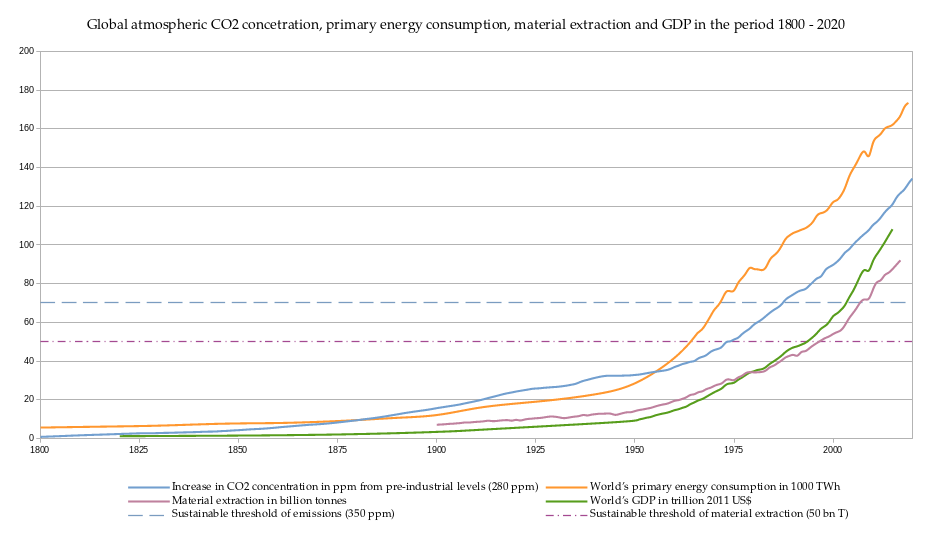
\includegraphics[width=1\linewidth]{./figures/energy_emissions_extraction_GDP} \caption[Historical emissions, energy consumption, material extraction, and GDP]{Historical growth of CO2 concentrations, primary energy consumption, material extraction, and GDP. Sources: material extraction — UN International Resource Panel and Krausman et al. 2009; historical and observed CO2 emissions — CO2 Earth; primary energy consumption and GDP growth — Our Wolrd in Data; sustainable threshold of emissions — 350.org; sustainable threshold of material exctraction — Bringezu (2015).}\label{fig:unnamed-chunk-2}
\end{figure}

While the effects might be long-lasting, the window for collective action to keep not only atmospheric greenhouse gas concentrations but also Earth's other biophysical processes such as biodiversity and phosphorus and nitrogen cycles within the boundaries of what is considered a ``safe operating space for humanity'' (\protect\hyperlink{ref-rockstrom_planetary_2009}{Rockström et al. 2009}) is counted in years and decades. As of November 2021, both the pledges and the more concrete nationally determined contributions (NDCs) by the signatories of the 2015 Paris Climate Agreement have set the world on a path of global temperature rise that will, by the end of this century, go well beyond the targeted 1.5°C above the pre-industrial levels (for the latest projections based on actual NDCs and policies, see \protect\hyperlink{ref-climate_action_tracker_cat_2021}{Climate Action Tracker 2021}). These NDCs are primarily pivoting around technological change, most of all on an energy transition away from fossil fuels, and are designed to avoid politically challenging interventions into the patterns of production, social needs, and redistribution of wealth, let alone into the larger-still patterns of intensive extraction from Earth's ecosystems. A notable role in these carbon-reduction scenarios is reserved for negative emission technologies (\protect\hyperlink{ref-anderson_trouble_2016}{K. Anderson and Peters 2016}). These technologies, meant to capture and store existing and future atmospheric CO2 emissions, have not yet reached maturity and, even if successfully developed, might never be deployed at the projected scale. Nevertheless, they are necessary to allow countries to legitimate their continued use of fossil fuels well into the 21st century until, so they pledge, renewables replace fossil fuels. Ironically, climate policies that are supposedly guided by political realism rely in these pledges on potentially unrealistic advances in technology. Be that as it may, a radical technological restructuring over the next decades seems inevitable. Either because the climate disruption unleashed by the continued use of fossil fuels will make large parts of the planet uninhabitable and will require significant societal and technological adaptation or because a planned and coordinated effort to exit from the fossil-fuel economy will make it so.

The main protagonist in these scenarios is thus technology. Technology serves both as the culprit and the saviour. And while climate change might have rattled the belief that technological modernisation is necessarily a progress in the right direction, technologies' central role in the public imaginary as a driver of social transformations has remained unchallenged. This techno-developmentalist worldview (\protect\hyperlink{ref-medak_technologies_2018}{Medak 2018}) is grounded in the way the history of previous transitions is commonly perceived. For example, the canonical narratives of the Anthropocene (cf. \protect\hyperlink{ref-crutzen_anthropocene_2000}{Crutzen and Stoermer 2000}; \protect\hyperlink{ref-steffen_anthropocene_2011}{Steffen et al. 2011}) --- the story of a geological age where the impact of human actions on Earth's subsystems has assumed planetary proportions --- typically start with the Industrial Revolution, presided over by James Watt's invention of the steam engine with a separate condenser and the transition to coal as a primary source of energy. While climate scientists do not fail to note that there were larger societal changes underway around the period, they understandably zero in on energy bottlenecks that purportedly limited social development before the onset of the fossil-fuel era. This functionalist approach allows scientists to focus on the narrower problem of greenhouse gas emissions. However, that does not set the historical record straight. Thus, to complicate the centrality that is allotted to technologies in the processes of historical change, in this chapter I will scrutinise the trajectory of past energy transitions, starting with the transition to coal and then to oil, to claim that the processes other than technological change catalysed significant aspects of the capitalist social metabolism.

The urgency of climate change enjoins us to look at how the historical processes of energy transitions actually unfolded. A lot is at risk in the coming decades and centuries if the technology-first approach proves to have been too inadequate and too untimely to prevent the worst consequences of climate destabilisation. Against the technology-first approach of policymakers, the following sections seek to ascertain that such \emph{transitions cannot be reduced to the replacement of dominant technological and energy systems but entail and require changes in social, economic, and political relations} (similar point is also made by \protect\hyperlink{ref-podobnik_global_2008}{Podobnik 2008}). This is particularly the case if these changes have to be directed against the existing cheap, abundant, and locked-in energy systems and if the significant reductions in existing forms of energy use are necessary to safeguard an ecologically livable and socially just future. By looking at both social and technological processes at play in the transition to ``fossil capitalism'' (\protect\hyperlink{ref-altvater_social_2007}{Altvater 2007}), at how they structured each other while transforming the ways in which the society harnesses energy and metabolises matter, I will argue that we can arrive at a better understanding of what were the multivariate processes of historical causation in the transition to fossil fuels. The salient point in my argument is that the relative weight of technological development, environment, social structure, and social agency changed over time as innovations, institutions, environmental degradation, and class antagonism impinged on each other.

Foundational for the interplay of these factors is the emergence of capitalism as a social formation. Starting from the positions of those historians who maintain that capitalism originated prior to industrialisation and the industrial use of fossil fuels, I will establish \emph{three defining aspects of capitalist formation that developed in relation to energy transitions}. Firstly, the transitions to first coal and then oil have cemented the central features of capitalism --- the separation of workers from the means of subsistence and the commodification of non-human nature, a process that started before the Industrial Revolution. Secondly, the growth dynamic achieved by emerging industrial capitalism could not be sustained without the continued colonial appropriation of human labour and land, which later consolidated into a neo-imperial world-system predicated on unequal exchange. Thirdly, the global expansion of capitalist social relations would not have been possible without fossil-fuelled technologies, just as fossil-fuelled technologies are not dissociable from the global expansion of capitalist social relations, resulting in a spiral of economic growth, expanding frontierism, and the extraction of energy and matter (to that spiral I return in section 7.2).

While this chapter outlines the historical interplay that has led to the formation of fossil-fuelled techno-capitalism, in the next chapter I will put forward a model to understand the lock-ins of the industrial capitalist social metabolism and strategic capacity of environmental groups and trade unions to disrupt and intervene into sociometabolic regimes in a way that is not limited to \emph{power from above} --- (i.e., actions of governments, (trans/sub)national governance structures, or capitalist enterprises) --- but equally includes disruptive \emph{power from below} (\protect\hyperlink{ref-piven_can_2008}{Piven 2008}) --- i.e., actions of organised labour, activists, scientists, educators or, simply, users.

\hypertarget{the-transition-to-capitalism-and-the-subsumption-of-nature}{%
\section{The transition to capitalism and the subsumption of nature}\label{the-transition-to-capitalism-and-the-subsumption-of-nature}}

\hypertarget{capitalism-before-industrialisation}{%
\subsection{Capitalism before industrialisation}\label{capitalism-before-industrialisation}}

Prior to the onset of industrialisation, larger changes were apace that set the stage for the transition to capitalism. Capitalism in Europe emerged under a number of enabling circumstances: stabilisation of borders inside the post-Westphalian Europe with the attendant imperial frontierism and plunder outside of Europe (\protect\hyperlink{ref-mezzadra_border_2013}{Mezzadra and Neilson 2013}); integration of national markets and expansion of overseas trade; mutual lockout between the Habsburg and Ottoman empires giving way to the Dutch and British hegemony (\protect\hyperlink{ref-anievas_how_2015}{Anievas and Nisancioglu 2015}); waning power of the Church, growing Enlightenment, rationalisation, and development of science; consolidation of individual and private property rights. However, capitalism as a historically specific mode of production did not evolve out of these circumstances.\footnote{For a definition of ``capitalism'' as a mode of production see Annex I.} Rather, as political economists Maurice Dobb (\protect\hyperlink{ref-dobb_studies_1947}{1947}), Robert Brenner (\protect\hyperlink{ref-brenner_origins_1977}{1977}), and Ellen Meiksins Wood (\protect\hyperlink{ref-meiksins_wood_origin_2002}{2002}) have argued in the seminal ``transition debate'' (\protect\hyperlink{ref-sweezy_transition_1978}{Sweezy, Dobb, and Lefebvre 1978}; \protect\hyperlink{ref-laibman_modes_1984}{Laibman 1984}), capitalism originated out of the specific property and class relations in the British countryside.

In the period 1350-1500, as a consequence of bubonic plague and peasant revolts, labour across Europe became scarce. Its value rose manifold, as did its access to feudal land. The shortage of labour and the growing power of labourers weakened the coercive power of feudalism, ending serfdom in many corners of Europe, and drastically improving the lives of the agricultural and urban proletariat (\protect\hyperlink{ref-marx_capital_1867}{Marx {[}1867{]} 2010, 35:666ff}; \protect\hyperlink{ref-federici_caliban_2004}{Federici 2004, 44}). Yet, by the end of that period, a backlash of repression and enclosures against the peasants overturned that process (\protect\hyperlink{ref-federici_caliban_2004}{Federici 2004, 68ff}; \protect\hyperlink{ref-hickel_less_2021}{Hickel 2021, 39ff}). Specifically in Britain, by the 16th century aristocracy was demilitarised and commanded a limited coercive power to extract surpluses from their tenants compared to its continental counterparts. However, it held a large proportion of land, made increasingly scarce for peasants by enclosures. Peasants now had to compete with each other for access to land, motivating the landlords to lease the land on a shorter-term leasehold basis. Variable rents, in turn, compelled farmers to work on increasing the productivity of land not to be outbid by competing farmers. This had the effect of pushing out the less successful from land, hence creating a class hierarchy between landholder rentiers, small agricultural entrepreneurs, and landless proletariat.

In the 17th and 18th centuries, this process generated a mutually reinforcing dynamic of growing agricultural productivity and growing demand for traded agricultural products that the landless proletariat depended on for its subsistence. The distinctive character of these emerging market relations regulating land, labour, and commodities was that their development was not grounded in the opportunity to buy cheaply and sell dearly as was the commerce hitherto. This was rather ``a type of market with no historical precedent'' (\protect\hyperlink{ref-meiksins_wood_origin_2002}{Meiksins Wood 2002, 102--3}), grounded in the dependence of large strata of society on the products in the market for their subsistence. Additionally, this process spawned a reserve army of labour that had no access to land and depended for its survival on selling its labour-power, a key pre-condition for the ensuing development of industrial capitalism.

The separation of landless peasants from the means of production portended a larger shift in the forms of social domination in the transition to capitalism, a shift from the personal power of the feudal lord over his subjects to the impersonal power of the market mechanisms over all social actors (\protect\hyperlink{ref-heinrich_introduction_2012}{Heinrich 2012, 203f}). Direct domination was supplanted by indirect domination through the ownership over the means of production, including land and tools, that landless peasants found themselves disappropriated of. Accumulation by dispossession and violence would thereby not disappear from the stage of history, nor the direct domination (or even ownership over people), but once separated from land and tools, the growing proletariat was set free, or rather had no choice but to seek waged-employment to survive.

\hypertarget{social-metabolism-of-agrarian-societies}{%
\subsection{Social metabolism of agrarian societies}\label{social-metabolism-of-agrarian-societies}}

Before industrialisation, the principal sources of energy were animal labour (including human), wind, water, and biomass. Clearing of natural vegetation, planting of staple crops, and improvement of farming techniques allowed peasants to actively utilise solar energy and increase the carrying capacity of land, the productivity of human and animal labour, and crop yields. Before the onset of industrial capitalism, agrarian societies in Europe were drawing around 40-70GJ of energy and 3-6t of materials per capita per year (\protect\hyperlink{ref-krausmann_global_2008}{Krausmann et al. 2008}). Such ``agrarian mode of subsistence'' (\protect\hyperlink{ref-sieferle_subterranean_2001}{Sieferle 2001}), though, did not allow for sustained long-term growth. Consecutive poor harvests would occur, soils would deplete, and local ecosystems would destabilise, generating diseconomies in the amount of labour that had to be invested in securing food and, in return, creating pressures on human wellbeing. Hence, agrarian economies tended toward stationary states (\protect\hyperlink{ref-sieferle_subterranean_2001}{Sieferle 2001, 191ff}). The capacity to utilise solar energy, the improvement of productivity of land, and the availability of mineral resources were limited, so the principal approach was conservation and reuse that maximised frequently scarce and intermittent resources.

Agrarian capitalism brought significant pressures on the environment. With the onset of commodity production, the monocropping techniques oriented at increasing crop yields, as well as the growing geographic distancing between where food is produced and where it is consumed, created a metabolic rift in the cycle of nutrients first observed by Justus von Liebig (\protect\hyperlink{ref-foster_ecological_2011}{Foster, Clark, and York 2011}). This rift had to be compensated for by adding increasing amounts of fertiliser brought from elsewhere, such as guano, whose fertilising properties were discovered in 1802 by Alexander von Humbolt in Peru, leading later in the century to a trans-continental trade in fossilised bird excrement (\protect\hyperlink{ref-cushman_guano_2013}{Cushman 2013}).

Similarly, the use of wood in furnaces for iron smelting, as well as for domestic use, led to large-scale deforestation, requiring that the use be strictly controlled. Amongst others by the introduction of wood theft laws, which the young Karl Marx famously wrote about for the \emph{Rheinische Zeitung}. Rivers and streams were the motive power of early cotton mills, the first truly accumulative capitalist industry. Mills required that the water flows be harnessed by dams, leading to a transformation of riverine habitats and a collapse of fish populations that hitherto provided a staple in the subsistence diet for much of the population (\protect\hyperlink{ref-steinberg_earth_2002}{Steinberg 2002a}). These physical and regulatory interventions were a continuation of the enclosure process that not only privatised the land but fenced off natural resources for particular uses while excluding others (\protect\hyperlink{ref-linebaugh_stop_2014}{Linebaugh 2014}), gradually transforming them to fit the needs of capitalist production --- a process that could be analogised to Marx's notion of ``formal subsumption'' (\protect\hyperlink{ref-marx_capital_1867}{Marx {[}1867{]} 2010}; \protect\hyperlink{ref-boyd_industrial_2001}{Boyd, Prudham, and Schurman 2001}). While these natural resources were being harnessed for production, they were still dominated by their geographically expansive and temporally intermittent profiles, thus limiting the patterns of intensive growth in extraction and accumulation. These limitations would only be overcome with the introduction of fossil fuels.

However, well into the 19th century the use of fossil fuels, of peat and coal, in Europe was largely for domestic use --- heating and cooking --- and was secondary to other sources of energy. At the height of the Dutch commercial power around 1650 peat peaked around 18\% of primary energy use (\protect\hyperlink{ref-fischer-kowalski_sociometabolic_2014}{Fischer-Kowalski, Krausmann, and Pallua 2014}). In Britain around 1700 coal stood only at 15\% of primary energy use (\protect\hyperlink{ref-krausmann_socio-ecological_2008}{Krausmann, Schandl, and Sieferle 2008}), its uptake driven primarily by deforestation. Even at the cusp of the Industrial Revolution in the 1830s, the domestic use accounted still for 46\% of the overall coal consumption (\protect\hyperlink{ref-mitchell_british_1988}{B. R. Mitchell 1988}; citation in \protect\hyperlink{ref-huber_energizing_2009}{M. T. Huber 2009}).

In agrarian capitalism the human hand was guiding the plough and tilling the land, and thus the means of production depended directly on human labour. Another transformation was necessary for the system of impersonal domination to be consolidated: the replacement of human labour by mechanised tools powered by inanimate sources of energy (\protect\hyperlink{ref-huber_energizing_2009}{M. T. Huber 2009}). At a scale needed for sustained growth that capital accumulation necessitates, that was only made possible by the development of the factory system and of the much more powerful prime movers such as turbines and steam engines powered by water or coal. The separation from the means of production and the generalisation of wage labour was not complete until those technology and energy transitions took off. The increasingly cheap energy driving industrial machines and suppressing human labour was the prerequisite for sustained capital accumulation and the expansion of capitalism to the rest of the world.

\hypertarget{the-transition-to-coal-and-the-subsumption-of-energy}{%
\section{The transition to coal and the subsumption of energy}\label{the-transition-to-coal-and-the-subsumption-of-energy}}

\hypertarget{the-transitions-prime-mover-class-struggle-or-technological-change}{%
\subsection{The transition's prime mover: class struggle or technological change?}\label{the-transitions-prime-mover-class-struggle-or-technological-change}}

So far I have outlined changes in the structure of social relations and social metabolism in the transition to capitalism prior to industrialisation and the introduction of fossil fuels, highlighting specifically two distinctive features of this transition: the changing structural character of human labour and the subsumption of non-human nature to capitalist processes. Next, I will argue that \emph{the ensuing transition to the industrial use of coal was not simply the result of technological innovations and coal's superiority as a source of energy, but of the interaction of class antagonism and technological change, and that the weight of causation shifted toward technologies as industrial development gathered pace}. Furthermore, I will contend that the transition to industrial capitalism and its much higher demand for energy and matter would not have been sustainable \emph{without the colonial appropriation of labour and land that subsidised --- both economically and ecologically --- its development}.

Capitalism is a system of self-perpetuating growth. As it grows, it ingests ever-greater quantities of energy and matter to produce more and more commodified goods and services. For this cycle of compounding growth to become truly continuous and grow at ever-larger geographic and metabolic scales, it requires sources of energy much denser than animate force, wood, wind, or water. The conventional narrative has it that it was the steam engine and coal that broke that bottleneck, marking the historical onset of industrial capitalism or even capitalism proper. In that account, capitalism has organically emerged out of the development of productive forces, and it is the technological advances that continue to be the prime mover behind its development. The role of organised labour in this transition to fossil capitalism remains but a footnote in a history of great inventions, in some accounts even a wrongheaded outburst of Luddite retrogradism (\protect\hyperlink{ref-mokyr_political_1998}{Mokyr 1998}). On closer inspection, that is not entirely correct. As I will argue, focusing on examples of disruptive power from below (which I ground theoretically in section 7.3.1), organised labour played a catalysing role.

In his \emph{Fossil Capital} (\protect\hyperlink{ref-malm_fossil_2016}{2016}), an extraordinary account of the origins of fossil capitalism in 19th century industrial Britain, Marxist ecologist Andreas Malm brings together a large body of evidence to show that the arrow of historic causation ran in the opposite direction of how the techno-determinist positions propose to view it. By remaining attentive to the social relations of production, Malm is able to discern what historiography (e.g. \protect\hyperlink{ref-sieferle_subterranean_2001}{Sieferle 2001}) has remained largely blind to: that there was no actual energy bottleneck at the moment when coal became the dominant source of energy and that the rise of coal cannot simply be attributed to technological advances or specific spatio-temporal properties of coal. The cycle of self-perpetuating growth initially appeared in the cotton industry, making it the first properly capitalist industrial sector. However, at the end of the 18th century, the primary source of energy in British and even US cotton mills (\protect\hyperlink{ref-steinberg_earth_2002a}{Steinberg 2002b}) was neither wood nor coal --- but water. The energy of streams and rivers, on which cotton mills were initially built, remained, in fact, more abundant, underutilised, efficient, and cheaper well after coal finally did become the dominant source of energy around 1835 (\protect\hyperlink{ref-malm_fossil_2016}{Malm 2016}, ch.~5), almost fifty years after Watt's invention. So, why did coal --- the energy of stock --- prevail over water --- the energy of flow --- if not for the superiority of coal as an energy source and the steam engine as a motive power?

Malm's analysis attributes the transition of industrial production to coal to a confluence of three major factors. Most prominently, the emergence of the organised labour movement as a consequence of the increasingly integrated factory production. The actions of the emerging labour movement led to the repeal of the Combination Laws in 1824, the Factory Act of 1833, the Chartist general strike of 1842, and the Ten Hours Act of 1847. These struggles and gains, however, left the water-powered capital in the countryside in an inferior position compared to the coal-fired capital in towns that could draw on a large reserve army of labour to hire and fire. The growing power of organised labour to make demands and limit the drudgery of factory work thus has made coal a better proposition for the capitalist.

Unlike water, coal was not bound to a specific location and, as a resource, did not need to be managed as a commons. It was not subject to the intermittence of the natural cycles of rain and drought. Regardless of its higher price, it afforded the factory owners more flexibility to act against organised labour and to compete against other capitalists. Thus coal's ``spatiotemporal profile,'' as a second factor, enabled capitalists to employ labour wherever and whenever it best suited their interests. Coal's capacity to abstract factory production from constraints of geography and weather made it ultimately more pliable to the process of accumulation, particularly as it enabled the development of rail and water transport. This pliability allowed capitalists to deploy machinery and automation to discipline the workers into an organisation of production that was fully apposite to the needs of capital. As Marx noted, ``the labourer becomes a mere appendage to an already existing material condition of labour'' (\protect\hyperlink{ref-marx_capital_1867}{Marx {[}1867{]} 2010, 35:389}). The shift from a merely formal to real subsumption of labour was thus accomplished.

Finally, the integration of coal into capitalist accumulation required that the energy source extraction itself becomes organised as a capitalist enterprise, extracted by the use of human labour, technologies, and energy --- and thus that its supply be made controllable. Unlike the energy of the flow that depended on seasons, the energy of the stock could be actively explored, extracted, and produced to follow the market demand and the needs of what Malm calls ``fossil capital.'' Fossil fuels thus enabled that energy itself becomes produced as a commodity and its production organised as an industrial capitalist enterprise. \emph{The capitalist relations of production have thus made the real subsumption of fossil fuels a prerequisite for their future development}. Fossil capital and its exceptional importance in the reproduction of capitalist relations was hence unleashed onto the world.

In \emph{Fossil Capital} Malm places class conflict, and not technological innovation or the superiority of an energy source, at the head of the transition to fossil fuels. Yet, as the capital adapts to the opposition and opts for technologies that undercut organised labour, the arrow of historical causation partly reverses. As I will argue in the next chapter, \emph{the technology, amplified through the mechanisms of the capitalist market, assumes no longer merely a catalysing but a strongly determining role.} An increasingly specialised and semi-autonomous process of technological development arises, leading from the Gilded Age of great inventors to corporate R\&D and publicly funded systems of techno-science, all partially separate from the relations of production in the factory (\protect\hyperlink{ref-fisk_working_2009}{Fisk 2009}; \protect\hyperlink{ref-braverman_labor_1998}{Braverman 1998}). The ensuing flurry of inventions set the tone for the techno-determinist worldview that already Lewis Mumford (\protect\hyperlink{ref-mumford_myth_1967}{1967}) detected as an outgrowth of that shift in the 19th century, a worldview that reduces human development to a function of technological development and that seems to remain hegemonic until today. For that particular period, though, that techno-developmental worldview was not completely unwarranted: with the real subsumption accomplished and the technological development seemingly promising endless progress (\protect\hyperlink{ref-scranton_determinism_1995}{Scranton 1995}), technology did become a distinct and significant factor of the historical acceleration of social modernisation (\protect\hyperlink{ref-rosa_social_2013}{Rosa 2013}).

\hypertarget{social-metabolism-of-early-industrial-capitalism}{%
\subsection{Social metabolism of early industrial capitalism}\label{social-metabolism-of-early-industrial-capitalism}}

The trajectory of fossil-fuelled industrial development unchained the social metabolism from the limits of the carrying capacity of a territory, agricultural productivity, and steady-state economy, leading to an exponential expansion in energy use and material extraction. The dispersed energy of solar flow was replaced by the concentrated energy of mineral stocks, now providing principal sources of energy for the production and circulation of commodities on which the satisfaction of social needs became dependent. Whilst the metabolic rates from modern energy carriers in the early industrialising countries around 1500 have been around 0.3 GJ/capita per year, by 1900 this rose to 85 GJ/capita per year (\protect\hyperlink{ref-fischer-kowalski_sociometabolic_2014}{Fischer-Kowalski, Krausmann, and Pallua 2014}). Fossil-fuelled industrialisation radically transformed the environmental, geographic, and colonial aspects of capitalist social metabolism.

Firstly, it scaled up environmental impacts: the anthropogenic processes no longer entailed only a geographically-limited depletion of resources, such as forests, soils, or animal populations, but \emph{now they attained indirect consequences at much larger scales through their wasteful side-effects such as air pollution, runoff of chemicals into soil, riverine and marine habitats, or inchoate greenhouse gas emissions}. The shift was from input-related to output-related impacts, creating pressures ``on the regional and global absorptive capacity of natural ecosystems'' (\protect\hyperlink{ref-krausmann_global_2008}{Krausmann et al. 2008, 644}). Capitalism revealed its double character: as an economic system of self-perpetuating value creation and a metabolic system of inflows of resources and outflows of waste. While natural resources extracted as inputs for production are part of the economic process, the indirect consequences of their extraction, production and consumption are not. However, both internal and external impacts are the result of the economic rationality of investment, prices and profits that governs capitalist development (\protect\hyperlink{ref-altvater_controlling_2014}{Altvater 2014}), and for as long as the resource depletion or environmental degradation does not impact the conditions of production that rationality will tend to prevail (more on capitalist rationality in section 5.6, on external and internal nature in section 7.2).

Secondly, agrarian capitalism's immediate effect was the expulsion of landless peasants into the cities in search for work, who settled there amidst the squalor of housing, soot, and sewage effluents (\protect\hyperlink{ref-engels_condition_1892}{Engels 1892}). The expulsion of peasants from land combined with the fossil-fuelled industrialisation to create a dynamic of rapid urbanisation that persists to the present day. Over the course of the 19th century, the population of Manchester grew by a factor of seven, of London by a factor of five, with over half of England and Wales urbanising by 1860. In the United States, from 1790 to 1860 urban population expanded by a factor of thirty (\protect\hyperlink{ref-steinberg_earth_2002a}{Steinberg 2002b}). \emph{Rapid urbanisation and industrialisation created a new degraded ecosystem of cities whose impact now reverberated through a network of metabolic links far across an increasingly global territory}. Metabolic processes in the cities were transforming hinterlands without a historical precedent, a process William Cronon memorably documented in his environmental history of Chicago as \emph{Nature's Metropolis} (\protect\hyperlink{ref-cronon_natures_1992}{1992}).

Thirdly, while industrial-capitalist social metabolism was marked by the transition from human labour as a prime mover to technologies fuelled by mineral sources of energy, personal domination continued to have a significant role in the metabolic viability of capitalist accumulation. Textiles were the first mass-produced capitalist commodity creating a growing demand for raw cotton. However, picking cotton in the fields was a labour-intensive process that could not be organised industrially. The shortage of labour in the New World colonies, once the Indigenous populations were decimated and the indentured slaves were freed to become farmers, combined with a growing demand for textiles to generate a pull factor for the slave trade with Western Africa. Slave labour in the Americas and colonial mercantilism in India subsidised the British industrial revolution with enormous transfers of cheap labour that would, if performed by settler populations or populations at home, have cost incomparably more. This amounted to a significant appropriation of embodied labour from Africa, the Americas, and India to the centre of the emerging capitalist world-system.

And it was also an appropriation of the productivity of land. To substitute with wool the cotton that Britain imported in 1830 would have required another 9.3 million hectares of pastures or almost 40\% of its entire territory (\protect\hyperlink{ref-pomeranz_great_2000}{Pomeranz 2000}). The growing demand for consumables such as sugar, tobacco, or coffee to keep the industrial populations fed and stimulated would have required additional cheap labour and land that were simply not be had in Britain. These imports were financed by exports of textiles and other industrial commodities, constituting an exchange between the zones with highly unequal values of labour and land, further made unequal by the imperial system of tariffs that effectively reduced India from a textile giant into a purveyor of cheap raw materials and importer of produced goods, consolidating within the emerging capitalist world-system a system of asymmetric economic and ecological unequal exchange (\protect\hyperlink{ref-emmanuel_unequal_1972}{Emmanuel 1972}; \protect\hyperlink{ref-hornborg_global_2012}{Hornborg 2012}).

Unleashing an enormous wasting of human lives, the colonial conquest led to the ``collapse of Indigenous ecologies'' (\protect\hyperlink{ref-merchant_theoretical_1987}{Merchant 1987}). It led to a reduction of diversity in ecosystems, the subsumption of agriculture to an industrial system of production, and a form of disciplining of labour whose methods would later be applied in the organisation of factories, laying the foundations for what Donna Haraway has proposed to call Plantationocene (\protect\hyperlink{ref-haraway_anthropocene_2015}{Haraway 2015}) --- a geological age defined by colonial legacies and continued racialised accumulation that troubles the conventional narrative of the Anthropocene centring on the Old World (\protect\hyperlink{ref-yusoff_billion_2018}{Yusoff 2018}) and modernity's fall from grace. \emph{This dependence of capitalist metropolis on cheap labour and transformable habitats in the colony paved the way for the future neo-imperial economic order, whose legacies are still detectable in the ``carbon colonialism'' of offset trading that constitutes a pillar of ecological modernisation}.

\hypertarget{the-transition-to-oil-and-the-globalisation-of-growth}{%
\section{The transition to oil and the globalisation of growth}\label{the-transition-to-oil-and-the-globalisation-of-growth}}

\hypertarget{the-governance-of-growth-and-the-institutional-foreclosing-of-systemic-change}{%
\subsection{The governance of growth and the institutional foreclosing of systemic change}\label{the-governance-of-growth-and-the-institutional-foreclosing-of-systemic-change}}

In the previous section I have argued that the weight of causation shifted from class conflict to technology as the technological advances integrated with the capitalist economy into a system of industrial production and later assumed an increasingly autonomous character. In this section, focusing on the transition to oil, I will complicate that assertion and bring in another historically emerging element to bear on the energy transitions --- economic and geopolitical governance --- to elaborate on how the transition to oil catalysed many institutional and metabolic features of the contemporary neoliberal capitalism characterised by highly wasteful energy systems that present significant obstacles for creating another, more sustainable and just metabolism.

To qualify that assertion with which I finished the account of the transition to coal, the arrow of causation did not \emph{lastingly} reverse in the opposite direction once fossil-fuelled industrialisation took off. Technologies, amplified through the capitalist competition, certainly became a more determining factor in social development, but the power of organised labour did not vanish under techno-capitalist domination. In fact, \emph{the conditions of industrial production created a concentrated and skilled mass labour force, enabling the labour movement to gain in capacity to disrupt capitalist processes and significantly reshape the emerging industrial states} (more on this disruptive power in section 7.3.1). After the transition to coal in the 19th century, the labour movement strategically used the chokepoints of fossil capitalism --- coal mines, railways, ports, and heavy industry --- to bring entire sectors of the economy to a standstill. Given that there was limited trade in coal across borders, that the transport of coal and goods depended largely on railways, that the blast furnaces could suffer significant damage if left without the coal feedstock, strikes and sabotage in the emerging industrial system had at their disposal instruments of significant bargaining power. As the political scientist Timothy Mitchell (\protect\hyperlink{ref-mitchell_carbon_2011}{2011}) argues, the period from 1870 on saw an unprecedented wave of industrial action sweeping across the industrialising world, with strikes of miners being more frequent and lasting than in any other industry. The labour movement embraced that vital position of agency to achieve momentous gains in labour, social, and democratic rights for the working class and society at large, making organised labour the determining factor in the development of democracies (\protect\hyperlink{ref-usmani_democracy_2018}{Usmani 2018}).

The initial decades of oil extraction saw, amongst numerous unrests, the 1905 revolution that was sparked off by oil worker strikes in Baku and Batumi and that managed to cripple the entire Russian empire. With the risk of the labour movement's disruptive power looming large, the oil barons and governments decided to conduct the oil transition in a much more coordinated fashion to minimise labour militancy. Oil's physical profile was conducive to such control: reserves could be tapped far from the sites of concentrated labour, extracted with fewer workers, and primarily using technology. Given its fluid form, oil could be moved flexibly by pipelines or ships, making it easily transportable and tradeable in the global market. For these reasons, the Truman administration did the oil industry's bidding and through its post-war recovery programs pushed the accelerated adoption of oil onto the rest of the world, and particularly Europe (\protect\hyperlink{ref-mitchell_carbon_2011}{T. Mitchell 2011, 29}). These developments had two immediate effects. Firstly, they globalised the energy system, characterised by the US's post-WWII control over the oil-producing territories and oil logistics, the denomination of oil prices in US dollars, and the US military hegemony. Secondly, they necessitated a new form of institutional regulation of the economy that would stabilise a highly volatile capitalist geopolitical environment, pacify the restless working classes at home, and create a geopolitical reality of economic interdependence.

As concerns the first effect, global capitalism emerged from World War II battered and threatened by the expansion of socialist projects across Eastern Europe and the post-colonial world. In order to stave off that threat, the US assumed the role of the capitalist hegemon. This hegemony received its institutional expression in the Bretton Woods system and the convertibility of other currencies against the dollar as the global ``reserve currency.'' However, with the US's towering productive capacity (left intact in the war, in 1952 it commanded around 60\% of all industrial production of advanced capitalist countries, cf. \protect\hyperlink{ref-hanieh_capitalism_2011}{Hanieh 2011, 30}) -- and with its overwhelming trade surpluses, the new Bretton Woods system quickly resulted in the inability of other countries to maintain trade balances with the US and a shortage of US dollars to buy goods. To counter this imbalance, the US set up its post-war reconstruction programs, such as the European Recovery Plan, aiming to transfer its surpluses abroad, bolster the destroyed post-war economies, and stabilise capitalism and its own international political leadership. The effect was an accelerated restoration of the productive capacities of Asian and European economies outside of the Soviet bloc. After the destruction of large swaths of capital stock in the war, the reconstruction programmes, and the technological transfer created conditions for a long period of growth in productivity, stable profit levels, and the development of free trade. Between 1948 and 1966, world trade grew at an annual rate of 6.6\% and between 1967 and 1973 at a rate of 9.2\% (\protect\hyperlink{ref-hanieh_capitalism_2011}{Hanieh 2011, 34}).

As concerns the second effect, amidst the post-war boom and its leadership expansion, the US was seeing an intense rise in labour militancy at home (\protect\hyperlink{ref-noble_forces_2011}{Noble 2011}). The legitimacy of demands for higher wages and full employment became increasingly difficult to recant. Therefore, the Truman administration decided to introduce reforms to economic governance that would have the lasting effect of curtailing the political efficacy of such demands. As Mitchell analyses in his article ``Economentality: How the Future Entered Government'' (\protect\hyperlink{ref-mitchell_economentality_2014}{2014}), in 1947 the Truman administration formed the Council of Economic Advisers (CEA). By the time the CEA published its 2nd annual report in 1948, the notion of the economy was changing its meaning in the public discourse --- the economy was no longer conceived of as a method of managing resources but as a dynamic system that was itself an object of policymaking. The CEA took it upon itself to monitor that system and to advise economic policymakers on how to steer it. This achieved several things: firstly, it placed the production of economic knowledge institutionally outside of the arena of democratic governance (\protect\hyperlink{ref-mitchell_economentality_2014}{T. Mitchell 2014, 490}). Secondly, it conjured up the economy as a dynamic system of interacting units, whose total value could be estimated by means of national income accounting and measured in gross national product. Its stability and growth had to be continuously maintained and shielded against any destabilising factors (\protect\hyperlink{ref-mitchell_economentality_2014}{T. Mitchell 2014, 485}). Thirdly, to express this dynamic instability, economic growth could not be represented as an exponential curve of cumulative growth that would have made evident the accumulating social wealth but rather as a more flat line of the rate of growth that always seemed constantly at risk of dropping. This epistemic choice effectively undercut the demands of the labour movement for a greater share of the existing social wealth and brought the popular demands in line with the interests of capital: a compact where labour could not demand the wealth that was already in existence but only a limited share of whatever growth was to be generated in the future.

From that moment of institutional and epistemic formalisation on, sustaining and spurring growth in a national economy became the central imperative and benchmark of political governance. One could even claim that the future, only decades earlier the temporal horizon of revolutionary transformation (\protect\hyperlink{ref-buck-morss_dreamworld_2002}{Buck-Morss 2002}), now mutated into an effort to maintain the social and economic order as stable as possible, limiting democratic interventions into the economy and effectively foreclosing the horizon of systemic change (to that foreclosed horizon of the future I will return in chapter 6). The Truman doctrine --- with its peacetime militarism aimed at consolidating its hegemony over the capitalist world, its development policy it promoted through international recovery programs, and the activities of Bretton Woods institutions --- injected this mechanism of economic governance into the rest of the capitalist world. It was this regime of governance, globalising what Karl Polanyi (\protect\hyperlink{ref-polanyi_great_1944}{1944}) analysed as the disembedding of market economy, that locked in the post-war world institutionally into the imperative of growth and the limitations it places on social transformation. And, as I will argue in chapter 5, \emph{it is this regime of governance that undercuts the ability of contemporary societies to respond to and mitigate the destabilisation of planetary ecosystems}.

\hypertarget{oil-and-economic-instability}{%
\subsection{Oil and economic instability}\label{oil-and-economic-instability}}

A fundamental characteristic of capitalist development is the growing geographic distancing between the location of production and the location of consumption. This separation creates commodity exchanges and metabolic relations between the town and the countryside, as well as between a town and a town in a network of towns. With the introduction of coal and oil, the circulatory system of goods, energy, and raw materials underwent a manifold speed-up, significantly reducing the turnover time, barriers to markets, and prices of commodities (\protect\hyperlink{ref-harvey_limits_2018}{Harvey 2018}). But equally, with the post-WWII logistics revolution, catalysed by the advances in containerisation and computerisation, this circulatory system enabled the creation of value chains of just-in-time production operating across ever-larger global geography. This circulatory system exploits differentials in prices and protections of labour and environment, frequently following old or creating new extraterritorial spaces of imperial, racialised, and militarised unequal exchange (\protect\hyperlink{ref-cowen_deadly_2014}{Cowen 2014}; \protect\hyperlink{ref-easterling_extrastatecraft_2014}{Easterling 2014}; \protect\hyperlink{ref-khalili_sinews_2021}{Khalili 2021}). Pivotal for this circulatory intensification was the transition from coal to oil.

Oil was a quintessential commodity of globalisation: it fuelled the global circulatory system, it was globally traded, and it bootstrapped globalised finance. By 1949 hydrocarbons accounted for 49\% and by 1960 for 72\% of all energy use in the US (\protect\hyperlink{ref-hanieh_capitalism_2011}{Hanieh 2011, 35}). The rest of the world was slower to transition, but by 1960 hydrocarbons became the globally dominant source of energy, peaking two decades later at around 60\% of all energy use (\protect\hyperlink{ref-ritchie_energy_2020}{Ritchie and Roser 2020}). In the 1950s, the world's production of crude oil expanded from 10 to 20 million barrels per day, continuing with rapid growth into the 1970s, by which time the Middle East's production surpassed that of Europe and North America combined (\protect\hyperlink{ref-hanieh_capitalism_2011}{Hanieh 2011, 36}). With a tide of anti-colonial liberation movements, the oil-producing countries would come together in 1960 to form the Organization of Petroleum Exporting Countries, assuming control over crude oil prices and nationalising their fields from the colonial oil companies. Acting through its regional ally Saudi Arabia, to whom it was providing military and political support, the US managed to secure that all trade in oil at least continues to be denominated in US dollars and that Saudi petrodollars be invested in ``US-denominated bank accounts, equities and Treasury bonds'' (\protect\hyperlink{ref-hanieh_capitalism_2011}{2011, 44}).

These developments had a profound effect on the geopolitical order and the emergence of a new global financial system. By the 1970s, the economic activity in the core of the capitalist system had slowed down. The over-accumulation resulted in high inflation and reduced profit rates. With the technologies of the immediate post-war period having become generalised, with the expectations of the social standard by the industrial workforce still rising, and with the capitalist expansion limited by the socialist and post-colonial national liberation movements, post-war capitalism was entering its first big crisis. The rising price of crude oil, particularly after the Arab-Israeli war in 1973 and the Iranian Revolution in 1979, which have unleashed two oil shocks, dramatically expanded the financial capacity of oil-producing countries of the Middle East and particularly of the Gulf region. Their reserves were primarily being invested in creating new financial markets (and so-called {``paper oil''} that now, instead of the physical supply, regulated the price of oil, cf. \protect\hyperlink{ref-altvater_social_2007}{Altvater 2007}), offering a novel way to avoid restrictions on government lending and baking reserve requirements. This set off an explosion in offshore shadow finance and credit activity that allowed multinationals to fully internationalise their operations and the developing countries of the South to gain access to affordable credit. However, once the energy prices doubled in 1979 and the Volcker Shock radically increased the interest rates to battle inflation, money became expensive for both corporations and countries. Structural adjustment programs were imposed by the Bretton Woods institutions, socialism started to collapse, markets were deregulated. After the oil boom arrived the neoliberal bust.

\hypertarget{cheap-and-stable-energy}{%
\subsection{Cheap and stable energy}\label{cheap-and-stable-energy}}

The dissemination of fossil-fuelled technologies was rapid. While in the 1800s, the world's fossil-fuel production stood at around 100, by 1870s it reached 1,850, by 1950s 21,000, and presently it is approaching 100,000 million tonnes of oil equivalent per decade (\protect\hyperlink{ref-pirani_burning_2018}{Pirani 2018, 10}). In Britain from 1800-1870 the installed capacity of motive power grew from 0.17 to 2.2 million horsepower (\protect\hyperlink{ref-mitchell_carbon_2011}{T. Mitchell 2011, 15}), powering steam engines, spinning jennies, and blast furnaces. The following decades saw the Second Industrial Revolution with innovations in electricity and internal combustion engines, so that by 1950 the installed capacity, powered mostly by fossil fuels, reached 22 million horsepower. This expansion has resulted in drastic increases in the social appropriation of energy and matter from nature. Presently, the average energy use in developing and developed industrial economies ranges between 100-400 GJ and material use between 15-25 tonnes per capita per year (\protect\hyperlink{ref-krausmann_global_2008}{Krausmann et al. 2008}, \protect\hyperlink{ref-krausmann_growth_2009}{2009}; \protect\hyperlink{ref-fischer-kowalski_sociometabolic_2014}{Fischer-Kowalski, Krausmann, and Pallua 2014}). The shift to mineral sources of energy cemented a metabolic spiral between industrial capitalist societies and planetary ecosystems premised on the high throughput of energy and matter. These processes are tied in with economic growth: since 1800, the world's Gross Domestic Product (GDP) has grown by a factor of a hundred, and the patterns of energy, emissions and material extraction have followed the trajectory of growth (see \emph{Figure 3.1}), making the prospect of decoupling the economic growth from environmental impacts highly dubious (see section 6.2.2).

This rapid metabolic expansion depended on a cheap and stable energy supply. \emph{Cheap energy has guaranteed that labour could be technologically either replaced or intensified to increase productivity, keep the competitive edge, and reduce wages, while at the same time ensuring that the prices of commodities, transport, heating, cooling, and cooking be kept down.} The principal instrument to cheapen energy are subsidies, in use since the early 1900s (\protect\hyperlink{ref-johnson_long_2011}{Johnson 2011}). A group of researchers (\protect\hyperlink{ref-coady_how_2017}{Coady et al. 2017}) has calculated that only in 2015 the global fossil fuel subsidies, with the largest part going to coal, stood at US\$5.3 trillion or 6.5\% of the global GDP. They suggest that eliminating subsidies would reduce greenhouse gas emissions by 21\% and air-pollution-related deaths by 55\%. Yet lavish subsidies have led to the continued development of inefficient, polluting, and wasteful energy systems that the world is now locked into.

The stability of supply in the present energy systems is designed to rely on the large, centralised power generation and the long-distance energy infrastructures such as grids, pipelines, and ports. Such an approach to stability created inadequate uses of energy that the physicist Amory Lovins, at the time member of Friends of the Earth, has once called ``hard energy paths'' (\protect\hyperlink{ref-lovins_soft_1979}{Lovins 1979}). Lovins' \emph{Soft Energy Paths: Towards Durable Peace} argued against the still-dominant view that societies need to sustain an ever-growing energy demand, which implies substantial inefficiencies, wasteful centralised energy generation, and militarised energy security. Lovins instead proposed to pursue ``soft energy paths,'' which would rely on renewable energy from the sun, wind, and vegetation --- and, importantly, \emph{energy conservation}. Soft energy paths would be built on flexible low-tech systems that could be installed by non-experts; systems that would be distributed, matching in scale, and produced close to the point of use; and systems that would match the energy quality to the end-use needs (\protect\hyperlink{ref-lovins_soft_1979}{Lovins 1979, 39}). For instance, a high-temperature nuclear reactor need not be used to heat a home at a much lower temperature, instead of using passive design, heat pumps, or solar panels, with smaller losses of energy in conversion and none in transmission. Technologies for ``soft energy paths'' were already available at the time of Lovins's writing. However, with Reagan's rabidly anti-environmental administration and the onset of neoliberalism, the subsidies for renewables and conservation of energy put in place during the oil shocks were dismantled. The world, particularly the US, continued on the hard energy path, contributing, amongst others, to the geopolitical destabilisation of the Middle East that since the 1990s has claimed the lives of almost a million people (\protect\hyperlink{ref-watson_institute_cost_2021}{Watson Institute 2021}). The soft path was not taken not because it was technologically unfeasible but because of the ``political economy of incumbency'' --- the governments were too tied in with the existing interests of fossil capital and unable to grapple with the issues of just transition (\protect\hyperlink{ref-newell_political_2018}{Newell and Johnstone 2018}), meaning that subsidising financially and militarily the hard path continued to present a politically easier path. \emph{Forty years later, energy policies are returning to decentralised and conservation systems, however still clinging to the imperative of growing the energy supply --- setting themselves up, as I will elaborate next, for a potentially impossible task.}

\hypertarget{the-next-transition}{%
\section{The next transition}\label{the-next-transition}}

\hypertarget{social-metabolism-of-destabilised-status-quo}{%
\subsection{Social metabolism of destabilised status quo}\label{social-metabolism-of-destabilised-status-quo}}

In this chapter, I have retraced the trajectory of technological changes, class struggles, and the institutionalisation of capitalist regulation that have interacted since the beginning of the industrial use of fossil fuels to create the contemporary energy systems, industrial-capitalist social metabolism, and the planetary ecological crisis. \emph{The central axes of analysis have focused on the application of fossil-powered machines to extend the separation of labour from the means of production, the continued colonial appropriation of labour and land, and the imbrication of capitalist growth with the growing throughput of energy and matter and its wasteful impacts.} I have argued that the fossil energy transitions were not simply technological but were driven by social antagonisms and institutional governance. In these concluding passages, I will begin to outline the challenges facing the current technology-first transition, claiming that its goals --- stabilisation of planetary ecosystems --- will unlikely be achieved without a significant change in the purposes and patterns of production and consumption, potentially leading away from the capitalist social metabolism.

Recently IPBES (\protect\hyperlink{ref-ipbes_global_2019}{2019}) warned that 75\% of land and 66\% of ocean biomes had been impacted by human action. This has had just as an unprecedented destabilising effect on Earth's biogeophysical subsystems: the biomass of wild mammals has been reduced by 82\%, the area of natural ecosystems by around 50\%, and a million species are at risk of extinction. At the same time, the greenhouse gas emissions are locking in the global temperature rise well in excess of 2°C with the accompanying sea-level rise and acidification of oceans. The phosphorus and nitrogen cycles have been dangerously disrupted, and a number of other biophysical indicators are approaching critical boundary levels beyond their Holocenic variability that has benefitted human societies (\protect\hyperlink{ref-steffen_planetary_2015}{Steffen et al. 2015}). Both IPBES and IPCC have called for urgent action, including ``transformative changes across economic, social, political and technological factors'' (\protect\hyperlink{ref-ipbes_global_2019}{IPBES 2019}) and ``rapid, far-reaching and unprecedented changes in all aspects of society'' (\protect\hyperlink{ref-ipcc_summary_2021}{IPCC 2021}).

That kind of action is not beyond doable. Among the ``Shared Socioeconomic Pathways'' used by the IPCC, the only cluster of scenarios that stays below 1.5°C temperature rise by 2100 is the SSP1, titled ``Taking the Green Road.'' This cluster includes scenarios where development respects environmental boundaries, growth shifts toward comprehensive human wellbeing, inequality is reduced across the board, and consumption is oriented toward low energy and material output (\protect\hyperlink{ref-oneill_new_2014}{B. C. O'Neill et al. 2014}; \protect\hyperlink{ref-hausfather_explainer_2018}{Hausfather 2018}).\footnote{These are still not degrowth scenarios, such as those proposed by \protect\hyperlink{ref-kuhnhenn_societal_2020}{Kuhnhenn et al.} (\protect\hyperlink{ref-kuhnhenn_societal_2020}{2020}) or \protect\hyperlink{ref-keysser_15_2021}{Keyßer and Lenzen} (\protect\hyperlink{ref-keysser_15_2021}{2021}), to which I will return in section 6.4.} Unlike other pathways, this SSP has both low mitigation and low adaptation costs. It is technologically doable because it does not bank on technologies. Yet, among all these aspects that comprise a pathway and that could be subject to policymaking, the latest COP26 Glasgow Climate Pact (\protect\hyperlink{ref-unfccc_glasgow_2021}{2021}) hinges largely on energy and technology changes: a gradual phaseout of coal, methane emission reduction from production processes, and modest environmental protection. Building on the liberal international order that developed in the post-war period, the COP meetings place a barrier on discussing systemic changes (see section 5.5). They are deemed politically unfeasible. The Overton window of permissible policy debate is largely fixed. Accordingly, faced with the urgency of the climate crisis, all the policymakers can debate are varying commitments to energy transitions and strategies for post-carbon growth. The policy challenge in these strategies is to see the environmental crisis as simply a technological challenge and an economic opportunity.

\hypertarget{challenges-of-the-next-transition}{%
\subsection{Challenges of the next transition}\label{challenges-of-the-next-transition}}

The next energy transition is observably underway. But while it is currently driven by the dropping prices of new renewables and the carbon pricing decarbonising power generation, much harder and slower tasks will be decarbonising manufacturing, housing, transport, and agriculture. The needed reduction to net-zero will be hard to achieve by 2050 given the current rates of growth in low-carbon electricity, carbon drawdown, or biomass. Concerning the expectation from technologies, Cambridge University engineering professor Julian Allwood (\protect\hyperlink{ref-allwood_technology_2021}{2021}) in his \emph{Financial Times} commentary of the COP26 meeting had the following to say:

\begin{quote}
Averaged over the world, we currently have 4kWh/day of electricity per person, growing at 0.1Wh/day annually. But the COP26 plans require 32 (range 16-48). We currently have 6kg of CCS per person per year, growing at 0.1kg/year annually, but the COP26 plans require 3,600 (range 1,400-5,700). We currently eat 100kg plant-based food per person each year, but producing enough bio-kerosene to fly at today's levels requires 200kg of additional harvest.
\end{quote}

\begin{quote}
In the 28 years we have left to reach net-zero emissions, there is no possibility that our supplies of electricity, CCS and biomass will scale to anywhere near the levels required by the plans discussed at COP26.
\end{quote}

Global energy transitions were never quick. At the global level, warns the prominent energy historian Vaclav Smil, energy transitions were always a gradual process (\protect\hyperlink{ref-smil_energy_2016}{Smil 2016}). It took 60 years for coal to go from 1\% to 50\% of the global share of primary energy supply; for crude oil to peak at around 40\%; for gas to peak at below 25\%. And while rapid national-level, end-use, or prime mover transitions have happened in the past (\protect\hyperlink{ref-sovacool_how_2016}{Sovacool 2016}), as in the case of the Dutch shift to natural gas, large economies with ``high per capita energy demand and with extensive infrastructures serving a well-established fuel demand, cannot accomplish the substitutions so rapidly'' (\protect\hyperlink{ref-smil_energy_2016}{Smil 2016, 27}). Given the size of global energy demand and the attendant infrastructure, as well as the huge sunken cost into the still-growing fossil sector and its reserves (\protect\hyperlink{ref-bp_energy_2021}{BP 2021a}), it comes as no surprise that the new renewables, in spite of the enormous gains in installed capacity, are struggling to maintain their share in the global primary energy consumption --- currently hovering around 5\% (\protect\hyperlink{ref-bp_statistical_2021}{BP 2021b}).

Importantly, Smil warns that the shift to renewables cannot be expected to proceed as exponentially as is assumed in the public debate. There is a number of constraints that are readily ignored: firstly, the innovation and deployment of renewables so far have been more of a linear than an exponential process; secondly, there are technological, biogeophysical, and environmental limitations to the upscaling of renewable sources such as old centralised transmission systems, lack of storage, limitations of mineral resources, intermittence of wind and sun; thirdly, the inertia of sunken costs in the existing energy system, its reliability, and the geopolitical wrangle present a further set of obstacles. Smil castigates as ``fictional'' scenarios such as those of Stanford engineering professors Jacobson and Delucchi (\protect\hyperlink{ref-jacobson_providing_2011}{Jacobson and Delucchi 2011}; \protect\hyperlink{ref-delucchi_providing_2011}{Delucchi and Jacobson 2011}), for not minding these constraints and what is needed for the level of rapid upscaling that they envision. Many, including \protect\hyperlink{ref-trainer_critique_2012}{Trainer} (\protect\hyperlink{ref-trainer_critique_2012}{2012}) and \protect\hyperlink{ref-zehner_green_2012}{Zehner} (\protect\hyperlink{ref-zehner_green_2012}{2012}), caution against such optimism. In fact, the global primary energy supply might remain dominated by fossil fuels even by the mid-21st century (\protect\hyperlink{ref-smil_energy_2016}{Smil 2016, 210}).

If we assess renewables for their capacity to substitute fossil fuels, only solar radiation operates at magnitudes on par and greater than the current global primary energy demand. Currently, however, wind turbines are supplying most of the renewable energy. But ultimately, much will hinge on developing both the distributed and centralised generation of solar power. Worryingly, the global investments in renewables are still towered by the investment in fossil fuels (\protect\hyperlink{ref-bp_energy_2021}{BP 2021a}). For Malm, this is an evident consequence of the fact that unlike the energy of the stock that provides opportunities for the long-term exploitation of labour, large corporations like Exxon, BP, Shell and their investors might not see enough economic interest in solar energy whose price is dropping steeply --- potentially, an energy system that does not secure long-term rents. In fact, as we have witnessed amid the energy and war crisis in the winter of 2021/2022, the lagging investment into renewables and growing carbon prices might result in significant instabilities of energy supply and energy price hikes.

The present energy system is locked in into large-scale generation, continued rise in energy demand, and inefficiencies in transport and conversion. However, a more expedient way to hasten the substitution of fossil fuels by renewables is by reducing the aggregate energy demand and shifting to an adequate use of energy. The less there is to substitute, the easier it is to substitute. This can be done either by improving the efficiency of energy use or by, as Smil suggests, moderating ``energy expectations'' (\protect\hyperlink{ref-smil_energy_2016}{Smil 2016}). Yet, while the most advanced economies have seen a gradual decoupling of growth and carbon emissions, their energy demand and carbon intensity have been largely offshored to China as the present-day ``workshop of the world.'' Although China has played a leading role in the build-out of renewables, it relies heavily on coal and, to a lesser degree, on oil and gas for its expanding manufacturing, infrastructure, and transport sectors, most of which are export-oriented. This transformation of the globalised system of production is not something that the consumers have to answer for, nor can they resolve it by their ethical consumption. Thus, I would contend that \emph{to achieve decarbonisation not only might the polluting societies need to limit the economic and energetic growth imperative to make a transition of renewables achievable in a few decades, but they might only succeed if they start to redefine the purposes of the globalised system of production.}

How future energy systems might shape out is a political choice and a choice laden with societal and systemic implications. Distributed renewables and electrification offer a potential for the localisation of production, conservation of energy, and uptake of communal transport. They offer an opportunity to reduce the displacement of ecological impacts onto other parts of the world. However, they might also offer an opportunity to end the separation of the worker from the means and ends of production by commoning energy generation (\protect\hyperlink{ref-dawson_peoples_2020}{Dawson 2020}). That, however, will not be achieved if the current transition remains only a matter of technological change, and not of a larger social and sociometabolic transformation. The following chapters are dedicated to conceptualising, documenting, and projecting into the future the agency of those actors that are proposing such alternative pathways of socially redistributive and sociometabolically transformative action. Before I do that, in the next chapter I will adumbrate the scale of the challenge that the industrial-capitalist social metabolism and its interlocking technological systems present for any rapid and far-reaching transformation.

\hypertarget{technology-and-agency}{%
\chapter{Technology and agency}\label{technology-and-agency}}

\minitoc

This chapter builds on the historical trajectory in the previous chapter to theoretically conceptualise the strategic capacity of actors such as activists, environmental groups, and trade unions to contest the sociometabolic status quo and the technology-first approach to resolving its problems in the context of the climate crisis. It theorises the scale of the present industrial-capitalist social metabolism and the mechanisms of its governance. Its principal objective is to dispel the notion that transition is simply a matter of pushing the best technological fixes to decarbonise the economy, but rather \emph{a matter of ideational and material struggles over the meaning and means of transition that involve wider social actors and constituencies, whose strategic agency is enabled and constrained by social structures dominated by the capitalist economy and the institutions of the state.}

This insight is relevant for understanding the type of agency of the organisations I will discuss later in this thesis. While in the next chapter I will treat them as epistemic and organising actors, straddling the institutional and social terrains of climate change politics, in this chapter I propose \emph{a model that indicates how the shift in the societal definition of the purposes of technological change through the framing of ecological modernisation opens up greater manoeuvring space for these actors to shape and transform the transition processes.} By drawing on three sets of theories that accentuate either agency or structure --- science and technology studies (section 4.2), strategic-relational approach (section 4.3), and critical theory of technology (section 4.4) --- the model works as an \emph{analytical framework} that combines their complementary insights to gain a \emph{comprehensive perspective} (\protect\hyperlink{ref-geels_micro-foundations_2020}{Geels 2020, 11}) on the problem of transformative interventions into the transition away from the thermocapitalist social metabolism.

My claim over the next two chapters will be that the discursive, institutional, and political contestations emerging from society's ``middle ground'' can directly disrupt the invisible operation of fossil infrastructures, shift the technology-first framing of environmental action, and even engage in the processes of social shaping of technology. However, this agency needs to be qualified and theoretically grounded, as not all actors have the same strategic power. The lock-ins into fossil-fuelled technologies (section 4.1) and the power asymmetries created by the social structures of the capitalist economy and the state (section 4.2) result in significantly diverging conditions for different social actors to effectively shape transitions.

To close off this chapter, I contend that despite the clear asymmetries of power between social actors, \emph{the dependence of ecological modernisation on socially-defined goals and the dependence of technologies on energy infrastructures make them susceptible to disruption in the form of sabotage, framing struggles, and bottom-up organising}, opening avenues for non-linear transformation instigated outside of the (trans/sub)national governance process (section 4.5). These forms of agency I will call \emph{vectors of disruption}.

\hypertarget{industrial-capitalist-lock-ins}{%
\section{Industrial-capitalist lock-ins}\label{industrial-capitalist-lock-ins}}

Before analysing how sociometabolic regimes and sociotechnical transitions can be disrupted and shifted, it is necessary to consider why the presently-dominant industrial-capitalist social metabolism is so entrenched that the efforts of (trans/sub) national governance to change its environmentally destructive footprint are failing to produce adequate and timely action? In the previous chapter, I retraced the historical origins of that social metabolism. As industrial development gathered pace in the 19th century, technology and energy systems became central to the reproduction of capitalist social relations and subject to an increasingly transnational economic and military governance. The growing system of capitalist production was set on a trajectory of continuous growth that necessitated an ever-greater extraction of energy and matter and an ever greater appropriation of non-commodified resources from nature.

This can be immediately intuited from \emph{Figure 3.1}. Over the last two centuries, and particularly since the beginning of the ``Great Acceleration'' after WWII (\protect\hyperlink{ref-steffen_anthropocene_2011}{Steffen et al. 2011, 805ff}), the economic output, demand for energy and materials, as well as polluting emissions have followed tightly correlated trajectories of growth, racing past the sustainable levels in the 1980s and 1990s. Many other sociometabolic factors not represented in the graph suggest the same exponential growth, most notably the transformation of the terrestrial biosphere, the expansion of industrial technomass, and the human population (see \protect\hyperlink{ref-steffen_anthropocene_2011}{Steffen et al. 2011}; \protect\hyperlink{ref-ellis_anthropogenic_2011}{Ellis 2011}; \protect\hyperlink{ref-hornborg_power_2001}{Hornborg 2001}). Since the mid-19th century, the use of energy-dense fossil fuels has enabled the development of a globe-spanning network of interlocking technological systems --- including those of manufacturing, infrastructure, transportation, agriculture, services, and communication --- that facilitate and require a continuously growing throughput of energy and matter. The accumulated scale of biophysical appropriation and the required technological base, still today powered up to 85\% by fossil fuels (\protect\hyperlink{ref-bp_energy_2021}{BP 2021a}), is enormous and presents a daunting obstacle for a transition to a less wasteful technological base and attendant social metabolism.

To account for the attained scale and quality of that technological base, the geologist Peter K. Haff (\protect\hyperlink{ref-haff_technology_2014}{2014}) has proposed that we decenter our anthropocentric view that sees technologies primarily in relation to human societies and that we consider the ``technosphere'' as an autonomous geological paradigm in relation to Earth's atmosphere, hydrosphere, lithosphere or biosphere, on whose sustained functioning human societies depend for their reproduction. The technosphere is already drawing on significant capacities of other geological paradigms, appropriating, for instance, over 10\% of their energy flux. The point Haff wants to make is that, given the dependence of contemporary societies on large-scale technological systems and the dependence of these systems on a high-rate throughput of energy and matter, the technosphere might not leave much strategic leeway to either human-centred or nature-centred policy initiatives. Human-built technology is so big and built around self-reinforcing mechanisms that it locks humans into a path of technological development that does not allow for significant shifts in its direction, scale, or dependence on resources. The planetary technosphere thus, in Haff's view, constrains the space of political decisions and social agency to change the direction of the present sociometabolic regime.

Haff's notion of the technosphere has been criticised for its truncated understanding of social agency. In response to his proposition that the technosphere has socially emerged but might no longer be socially controllable, a group of prominent Earth system scientists (\protect\hyperlink{ref-donges_technosphere_2017}{Donges et al. 2017, 26}), have criticised Haff for ignoring the fact that the technosphere has co-evolved with the ``collective agency of social macrostructures'' and that it continues to be sustained through a dynamic coupling with social and ecological structures. Macro-social structures continue to provide ``critical control points'' that can trigger non-linear, transformative changes in large-scale technological infrastructures. While, in their view, the agency of social actors at the individual (and organisational) level cannot directly impact the technosphere at the scale that matters for the destabilised Earth system, actions oriented at states, intergovernmental institutions, regulations, and economic entities indirectly can.\footnote{I would also add that the dependence of large-scale technological systems on other technological systems makes them also vulnerable to disruption by direct action. I will return to that below.}

Haff's view, I would contend, is deterministic. There are three assumptions that come together in deterministic framings of technological change. Firstly, the assumption that technological change proceeds largely autonomously from the social, political, or even economic factors, following primarily the considerations of technical efficiency, the cues of engineering ingenuity, and the affordances and limitations imposed by other technological systems (this last aspect receives in Haff's account planetary proportions). Secondly, the assumption that technological development is a succession of incremental innovations and radical breakthroughs where wrong turns, dead ends, and major catastrophes have little significance for the course of progress. Thirdly, the assumption that technologies are paramount catalysts of social change and can be relied on to produce solutions to major societal problems. Historically, such notions of \emph{hard} technological determinism emerge from the spurt of innovations that have driven the immense expansion of industrial capitalism since the 19th century (\protect\hyperlink{ref-mumford_myth_1967}{Mumford 1967}), the rise of a hegemonic capitalist system of production premised on competitive gains from technological innovation (\protect\hyperlink{ref-postone_time_1995}{Postone 1995}), and the separation of the technoscientific process from the immediate process of production (\protect\hyperlink{ref-marx_economic_1857}{Marx {[}1857b{]} 2010}). The period of major technological advances between the 1870s and the onset of the nuclear arms race have, particularly in the US, instilled a sense that technology enables endless social progress (\protect\hyperlink{ref-scranton_determinism_1995}{Scranton 1995}; \protect\hyperlink{ref-smith_technological_1994}{Smith 1994}). Regardless of a long tradition in social theory to criticise determinism, starting with William James (\protect\hyperlink{ref-james_dilemma_1884}{{[}1884{]} 1970}), technological determinism nonetheless reflects a hegemonic common sense even today, shaping motivations and expectations of technologists, investors, governments, and the public, and thus has to be acknowledged as effective at least at the justificatory level (\protect\hyperlink{ref-wyatt_technological_2008}{Wyatt 2008}).

But beyond being a hegemonic common sense, there are historically evolved objective factors that I propose we should nonetheless consider before we declare determinism entirely inadequate to understanding how technologies and societies co-evolve:

There is the \emph{scale} of thermocapitalist technomass that is hard to decarbonise and dematerialise --- large segments of accumulated technological base built since the Industrial Revolution have to be replaced and retrofitted in a few short decades. A number of \emph{material} challenges have to be overcome in the transition. For instance, the replacement of fossil-fuel systems with clean energy systems requires levels of material extraction to build turbines, panels, or batteries that might not be met with the existing reserves nor without alarming levels of extractive incursion on ecosystems and indigenous communities (\protect\hyperlink{ref-hickel_limits_2019}{Hickel 2019b}; \protect\hyperlink{ref-riofrancos_resource_2020}{Riofrancos 2020}). Or for instance, iron smelting requires coal while plastics manufacture depends on petrochemicals, and these feedstocks could be difficult to replace at the present scale despite early advances in renewable feedstocks. To circumvent these challenges requires either a substantial re-engineering of technological systems, a development of new technologies to extract from low-ores, a rapid expansion of renewable feedstock production --- or, maybe, a substantial change in the patterns of use and demand for those technologies. To add to the problem, throughout the energy transition, the availability of \emph{energy} has to be stable and --- according to the dominant orientation of ecological modernisation --- drastically increased to enable continued growth.

In addition to the scale and the corresponding glut for resources, the next constraining factor is that technological systems depend for their operation on other \emph{technological systems and infrastructures} (\protect\hyperlink{ref-hughes_networks_1993}{Hughes 1993}). As a technology grows in its maturity and scale, its replacement with another set of technologies requires a substitution of large accompanying and underlying infrastructures. This is currently the case with the replacement of internal combustion vehicles with electric vehicles that require charging stations and are as clean as the electricity they consume.

Furthermore, sociotechnical transitions are also constrained by a number of functions that technologies perform in the \emph{capitalist economy}. Firstly, innovation responds to the class conflict between labour and capital. For instance, replacing workers with robots can frequently be less productive, but it reduces the capacity of workers to disrupt the production process, organise and, thus, claim better wages and rights (\protect\hyperlink{ref-noble_forces_2011}{Noble 2011}). Secondly, innovation is driven by the competition between individual capitals aiming to achieve productivity gains. The introduction of new technologies can lead to a temporary increase in profits for an individual capital, but it is quickly caught up with. This dynamic produces an ever-greater magnitude of social material wealth yet keeps the value gains around average and the valorisation process constantly going (\protect\hyperlink{ref-postone_time_1995}{Postone 1995}). Thirdly, innovation can result in lowered prices or new commodities, entrenching particular technologies through market demand. Fourthly, technological cycles of innovation are backed-up by financial cycles of investment. Once the profit gains from a previous round of technological innovation start to taper off, the financial capital moves on to seek investment in new technologies that promise new expansion (\protect\hyperlink{ref-perez_finance_2011}{Perez 2011}). Fourthly, advances in innovation can shift larger or smaller quantities of profit from the productive to commercial or financial capital and vice-versa. All these processes intensify technological change yet drive it toward a limited set of social ends --- defined by class conflict, competition between capitals, and financial cycles, limiting in return the development of technological alternatives and reinforcing capitalism's hold on social development. As the economic historian Robert Heilbronner suggests, technologies might not be deterministic in the hard sense, but they do ``make history'' through the mediating structure of the capitalist economy, which has significant determinative effects on social structure (\protect\hyperlink{ref-heilbronner_machines_1994}{Heilbronner 1994a}, \protect\hyperlink{ref-heilbronner_technological_1994}{1994b}).

These were the lock-ins disaggregated into their material, energetic, technological, and economic components. Yet, how do they come together to form a self-reinforcing society-technology-nature nexus at the world-system scale that the environmental historian Jason W. Moore has called a world-ecology (\protect\hyperlink{ref-moore_capitalism_2015}{2015})? Another human geographer, Alf Hornborg (\protect\hyperlink{ref-hornborg_power_2001}{2001}), in his singular work in the anthropology of technology, investigating how in various social formations powers-that-be use technologies to appropriate the social surplus, has argued that industrial technologies combine three factors: the appropriation of embodied labour and natural resources, technical systems and attendant technical knowledge, and, decisively, the social relations of exchange. Building on the work of political economist Arghiri Emmanuel (\protect\hyperlink{ref-emmanuel_unequal_1972}{1972}) on uneven development, Hornborg posits that money, as a symbolic structure mediating exchange between unequal economies, enables a technologically more advanced economy to appropriate embodied labour and natural resources from a technologically less advanced economy at substantially lower prices than the prices the latter has to pay for the commodities produced by the former. What seems like a trade-in equivalent economic units is a trade of biophysically highly unequal quantities. A developing economy has to sell its labour and resources cheaply to buy advanced industrial technology dearly, pushing it down the spiral of underdevelopment and forcing it to absorb the environmental externalities of that process of extraction. These uneven ``terms of trade'' that create cheap inputs are central to the functioning of large-scale technological systems and industrial capitalism. Thus, Hornborg provides us with an important insight: the technological base premised on high intensity of material and energy flows and the economic unevenness are mutually reinforcing (\protect\hyperlink{ref-hornborg_ecological_2014}{Hornborg 2014}). Advanced industrial technology is premised on an unequal social world and degraded nature. Thus, changing one of the three might require changing the other two --- doing ecological justice might require changing both technology and social structure.

There are thus at least five historically evolved lock-ins that place \emph{soft} yet significant constraints on an urgent transition to equitable sustainability. A consequence being, as I want to put forward, is that \emph{ecological modernisation has to contend both with continuing these sociotechnical lock-ins and restructuring the fundamental elements of their operation --- and this contradictory task creates an opening for re-orienting the sociotechnical transition in another direction.}

These contradictions emerge once technological change can no longer be socially, institutionally, and politically framed --- as it was in the technological modernisation paradigm --- as a spontaneous process of technological evolution where innovators and entrepreneurs seize opportunities provided by the capitalist market and the regulation remains neutral to the general direction of that evolution. And that is the case with the ecological modernisation paradigm. It is a ``goal-oriented'' and coordinated process that strives to achieve sustainability at the societal and inter-societal levels (\protect\hyperlink{ref-geels_disruption_2018}{Geels 2018}). \emph{This change in framing --- and this is my central assumption in this chapter --- significantly changes the shaping, transformative, and determinative capacities of social actors and structures over the process of transition}. It opens up space for strategic agency to impact the direction of sociotechnical change and potentially shift the sociometabolic regime in significant ways.

The changes in capacities as the framing changes from technological to ecological modernisation are indicated in the model presented in \emph{Figure 4.1}. In this model, strategic agency is enacting social structures and is strategising to transform them, while, in turn, social structures are selectively enabling and constraining the actions of various social actors. Social structures include regulative processes institutionalised through the state, while social agency, for the purposes of my analysis, includes blockades, framing struggles, and organising as forms of disruptive action. In the technological modernisation framing, social actors have a relatively weak, social structures a stronger, and the capitalist markets a determinative shaping power over technological change. The capitalist economy also exerts a determinative effect on social regulation through the dependence of societies on commodity production for the provision for social needs and on capitalist accumulation for stability and taxes, both highly correlated with technological change. Once the framing shifts to ecological modernisation, with its goal-oriented transition, the shaping capacities of the capitalist economy over technological change get weakened, as its impacts on the planetary environment impose imperative goals of environmental action on societies, which in turn have to undertake stronger regulative interventions and transformations. On the other hand, the strategic capacity of middle-ground actors gains greater shaping and transformative power as well, as a window opens for ideational and material struggles over sociotechnical and sociometabolic transitions.

The rest of this chapter is dedicated to theoretically grounding elements of that model and conceptualising the opening for disruptive agency created by these changes in valences.

\begin{figure}
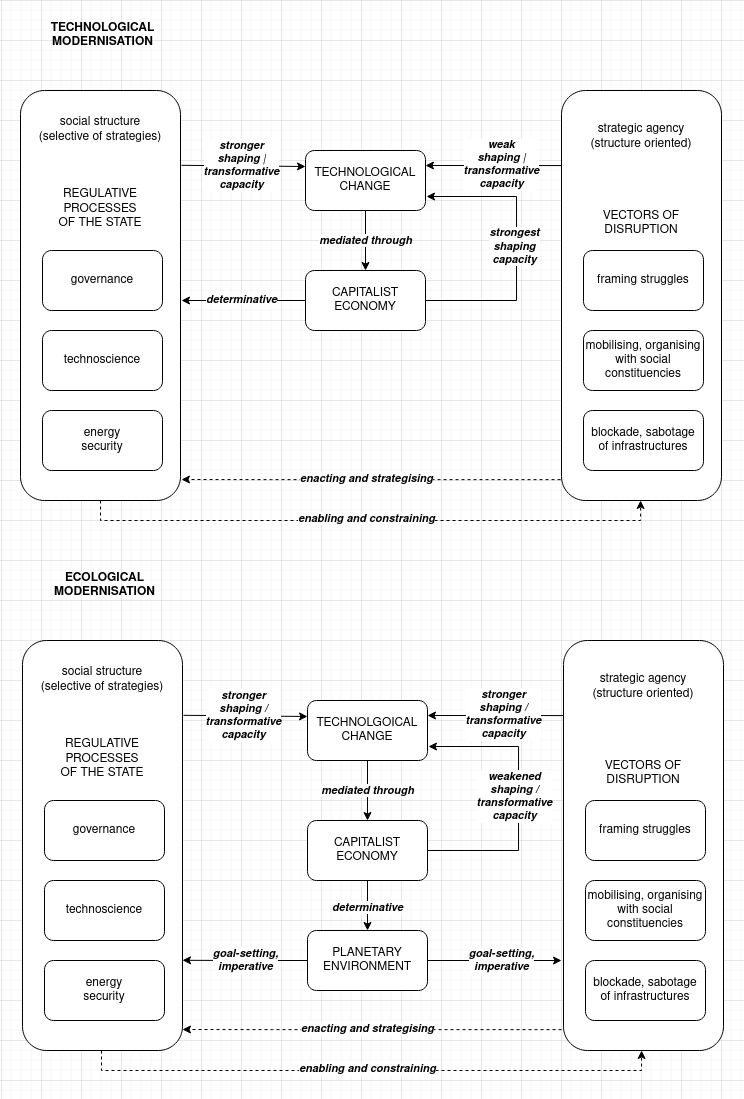
\includegraphics[width=1\linewidth]{./figures/technology_structure_agency_modernisation} \caption[Technological vs ecological modernisation]{Shifts in the shaping and transformative capacities in the transition from technological to ecological modernisation.}\label{fig:unnamed-chunk-3}
\end{figure}

\hypertarget{agency-in-sociotechnical-transitions}{%
\section{Agency in sociotechnical transitions}\label{agency-in-sociotechnical-transitions}}

The theories of sociotechnical transitions posit that an incumbent sociotechnical regime transforms through accumulated niche innovations and openings created by upheavals in the broader social and environmental context within the so-called sociotechnical landscape (\protect\hyperlink{ref-geels_micro-foundations_2020}{Geels 2020}). Interactions between the regime's institutions, technological innovation processes, and external shocks are marked by, amongst others, discursive, institutional, and political struggles that define the direction of a sociotechnical transition. In the model presented in \emph{Figure 4.1}, these struggles unfold between the social structures, capitalist economy, and strategic collective agency, all working to impact technological change. The strategic capacity of environmental groups and trade unions to steer the future transition to a post-capitalist social metabolism unfolds on the terrain of those struggles. Over the next three sections I will theoretically conceptualise that strategic capacity from the perspectives of social agency, social structure, and power.

Haff's radical autonomisation of human-made technology into a geological paradigm is the exact inverse of the dominant approach in science and technology studies (STS) that is focused on dissolving the separations between nature, social agency, and technology. This body of scholarship, emerging largely in the 1980s with the consolidation of the social construction of technology (SCOT) and the actor-network theory (ANT) research programmes (\protect\hyperlink{ref-latour_laboratory_1986}{Latour and Woolgar 1986}; \protect\hyperlink{ref-bijker_social_1987}{Bijker, Hughes, and Pinch 1987}; \protect\hyperlink{ref-haraway_simians_1991}{Haraway 1991}; \protect\hyperlink{ref-mackenzie_social_1999}{MacKenzie and Wajcman 1999}; \protect\hyperlink{ref-law_aircraft_2002}{Law 2002}), has opened up new, highly productive inroads into the social study of technoscientific processes, which it regards as dynamic networks of associations between a range of entities: human actors, artefacts, and non-human nature. By going back to some of the principal tenets of this scholarship, \emph{I want to highlight that social and technological systems are entangled in such a way that a change of interpretation and composition of technological systems can cascade to a social change, and that that agency is a capacity that emerges from relations and interdependences in those entanglements}.

Arguably the field's most prominent protagonist, Bruno Latour has contended that there is a developmental continuity between the social and the technological: once experimental and unstable associations between various entities --- both human and non-human --- become durable, they become technology (\protect\hyperlink{ref-latour_technology_1990}{Latour 1990}). The laboratory starts as an association between a microbiologist and bacterial culture to congeal into a stable assemblage that can be considered a technology (\protect\hyperlink{ref-latour_pasteurization_1993}{Latour 1993b, 73}). Along the same line of reasoning, the sociologist Michel Callon has proposed a reversal of perspective in sociological inquiry to suggest that engineers elaborating radical innovations are engaging in sociological analysis and thus studying technology development allows us to observe ``society in the making'' (\protect\hyperlink{ref-callon_society_1987}{Callon 1987}). The processes of experimentation and innovation in thoroughly technologised modern societies are thus constructive of new relations.

In the STS scholarship, technological change is conceptualised as collective sense-making, whereby different social groups engage in negotiating the form and function of a new artefact until it has attained a stabilised interpretation and use (\protect\hyperlink{ref-bijker_bicycles_1997}{Bijker 1997}). Thus, STS accommodates and emphasises the participation of different social actors in the process of technological change, ranging from policymakers, the public, producers to users, all of whom partake in negotiating interpretations and thus shaping technologies. This makes insights from the STS scholarship particularly useful for analysing the strategic agency of organisations that are neither corporations nor regulators to impact the direction of sociotechnical and sociometabolic change. In two ways:

Firstly, a reinterpretation of technologies' purposes and uses can have a transformative social effect. In an exemplary exposition of actor-network theory, Michel Callon (\protect\hyperlink{ref-callon_techno-economic_1990}{1990}) analyses techno-economic entities consisting of texts, technical objects, human skills, and money that constitute networks of associations in the production of goods and services. In such networks of associations, any intermediary that identifies and organises other intermediaries into a process of translation that articulates and addresses a problem is an actor that defines the network. Boundaries of networks are not stable --- various intermediaries might contend for the authorial role of the network-defining actor, and the networks only become consolidated through the processes of convergence of translations until such moment is reached when they attain complete stabilisation and can be taken as black-boxes with a settled interpretation of their agency. Importantly, once they have stabilised, these black-boxes --- markets, regulatory institutions, specialisations --- can easily collapse if a new technology or a new interpretation comes along and recomposes the existing networks of associations. For instance, solar power generation, if reinterpreted along the ``soft energy path'' (see section 3.5), can open up avenues for proposals of building distributed, citizen-owned energy system, where significant downscaling, communication of ownership, and redistribution of power becomes possible (see section 7.5.2).

Secondly, agency itself, a central concept to STS, is a capacity emerging through associations. Agency does not inhere in entities, but in relations as capacities constituted through their interactions (\protect\hyperlink{ref-latour_technology_1990}{Latour 1990}). Agency is, thus, not allocated by pre-defined positions in a social order but constituted in relations and actions. Agential relations are relations of mutual enablement or disablement between interacting entities. This theoretical schema of agency offers distinct advantages in social analysis: it remains close to the material reality and dynamic processes of (de)stabilisation and (re)constitution; social entities at micro-, meso- and macro-levels are analysed as isomorphic; and there is no separation of epistemological and ontological properties. Such empirical relationalism has spawned a number of new theoretical forays in science and technology studies, anthropology, or political science. Some of the most interesting have come from the scholars working in the tradition of feminist epistemology, for instance, in the form of new materialist theories of agential realism by Karen Barad (\protect\hyperlink{ref-barad_posthumanist_2003}{2003}), which attempts to supplant the representationalist binary between things and words with a process of differential becoming where objects and subjects that do not exist prior to their relation emerge through agential cuts from the intra-acting matter. Or, of the inter-species hybridity by Donna Haraway (\protect\hyperlink{ref-haraway_staying_2016}{2016}), which militates for making kin with other species in order to create refuges for multispecies survival in the period of Anthropocenic instability and pursue new biological-cultural-political-technological recompositions. By decentering the perspective away from the human, actor-network theory, and some varieties of post-humanist theories that have emerged in its wake, have gained an appeal in the epoch of climate change. As the feedback loops between sociotechnical infrastructures and Earth subsystems are gathering force, the notion that humans cannot be understood as the sovereign agents controlling the hybrid constitution of textual, technical, natural, or economic composites they produce or mobilise seems to be correct on its analysis (\protect\hyperlink{ref-latour_facing_2017}{Latour 2017, 62}).

However, these two salient insights of STS scholarship --- that agency is constituted in relations and that stabilised social orders can be destabilised by reinterpretation of technologies --- need to be critically bracketed. I will highlight three reservations: an inadequate understanding of the emergent properties of higher-level social structures, a disinclination toward antagonisms and distributive conflicts, and a counterintuitive expansion of the notion of agency.

STS scholarship tends to share a concern for destabilising the dualisms between the (categories of) subject and object, human and non-human, society and nature, rational and irrational, macro and micro (\protect\hyperlink{ref-latour_technology_1990}{Latour 1990}). Criticising the modernist dualisms that exclude from the realm of political representation a plethora of new assemblages and hybrid entities that modernity has spawned by combining social, natural, and technological processes, Latour has developed a counterproject to traditional sociology. In his view, traditional sociology has stabilised the meaning of the social as a form of causality that explains away the specificities of those assemblages by using the generic concepts of society, power, or capitalism that represent tautological ``black-boxes'' (\protect\hyperlink{ref-latour_we_1993}{Latour 1993a}). The use of these concepts, in his view, does not contribute to sociological analysis. He rather proposes to do away with ``the social'' and develop a sociology that would take on the task of closely following the associations and, from there, reassembling the social. A methodological priority of Latour's project is not to impose an explanatory or normative matrix onto the social, but rather to lend a listening ear to the actors and start from their understanding of reality (\protect\hyperlink{ref-latour_reassembling_2007}{Latour 2007}).\footnote{Following this commitment, Latour has launched acerbic attacks on critical theory, claiming that its proponents are patronising toward people at whose positions they direct their critique, duplicitous in their methodology as they selectively combine antifetishism, positivism, and realism, and working with ill-conceived concepts of society, discourse, capitalism (\protect\hyperlink{ref-latour_why_2004}{Latour 2004}; also \protect\hyperlink{ref-trexler_integrating_2013}{Trexler 2013}). Concerned by growing climate denialism and the hubris of Enlightened reason, Latour dishes out his critique by comparing critical theory with conspiracy theories. Yet, this is where Latourian theory starts to show its blind spots: it has difficulties to account for its own political concerns and alliances because they are shaped by the very macro-social structures it disparages so easily. For instance, a large body of research on climate denialism indicates that the strongest denialist demographic in the US by a significant margin were ``{[}f{]}iscally conservative white males {[}who{]} have disproportionately occupied positions of power within our economic system'' (\protect\hyperlink{ref-mccright_cool_2011}{McCright and Dunlap 2011}). Capital and power define the climate scepticism and misinformation. At the same time, the global population is largely expressing concern over climate change (\protect\hyperlink{ref-capstick_international_2015}{Capstick et al. 2015}).}

The problem is that narrowly empirical commitments fail to engage and take an oppositional stance to the black-boxed structures that drive asymmetries of power. Of late, Latour has changed his vocabulary to acknowledge inequalities, deregulation, globalisation, and capitalism as roots of denial and environmental destruction (\protect\hyperlink{ref-latour_earth_2018}{Latour 2018}; \protect\hyperlink{ref-latour_climate_2019}{Schouten 2019}). Latour's position against critique is, however, not shared by the entire STS field, as the sociology of translation that ``follows the actors'' can very well work as a critique of ``black boxes'' that need describing and unpacking, as was exemplary demonstrated in the anthropologist Anna L. Tsing's \emph{Friction: An Ethnography of Global Connection} (\protect\hyperlink{ref-tsing_friction_2005}{2005}), a study of translations that articulate together the capitalist and non-capitalist labour in the global capitalist value chains. Therefore, I would argue that \emph{macro- and meso-social structures need to be understood as emergent properties of lower social processes with their own organising logic that has enabling and constraining effects on the lower-level interactions}. In short, structure matters. However, the bias for narrow empiricism pushes ANT to readily disregard such higher-level social structures and their attained historical specificities (\protect\hyperlink{ref-elder-vass_disassembling_2015}{Elder-Vass 2015}). It is necessary to distinguish qualitative differences of social structure and economic power from agency.

Secondly, when focusing on deeply material micro-scale processes, as \protect\hyperlink{ref-martin_science_2012}{B. R. Martin, Nightingale, and Yegros-Yegros} (\protect\hyperlink{ref-martin_science_2012}{2012}) argue, the STS tends to privilege cognitive, cultural, and ideational forms of agency as opposed to confrontational forms such as strategising, struggles, and distributive conflicts that, as I will argue later in this and in the next chapter, are fundamental to environmental politics. Relatedly, the STS practitioners (\protect\hyperlink{ref-geels_micro-foundations_2020}{Geels 2020}: 11) point out that research in STS is more oriented to studying the early stages of elaboration, experimentation and composition of new assemblages and less toward studying how the existing sociotechnical regimes and assemblages are reproduced, destabilised, and overthrown, therefore requiring field-level and structural analysis. Given the potential failing of the technology-first strategies in climate policy, the disruption and sabotage of existing technological systems might have, in the urgency of climate action, equal if not greater importance than the elaboration of new sociotechnical regimes. As do struggles over the material implications of the transition, to start with. Sabotage, organising, and framing struggles matter just as the engineer-driven process of innovation does.

Lastly, the isomorphic ascription of agency in assemblages to humans and non-humans, be they non-living nature, human-built artefacts, living organisms, or symbolic structures, is consequential within the framework of ANT. This proposition attempts to break away from anthropocentric exceptionalism and acknowledge other-than-human agencies that are not grounded in the subject-object separation. However, equating human and non-human agencies is highly counterintuitive, so much so that it has been criticised by many STS proponents (most prominently in \protect\hyperlink{ref-collins_epistemological_1992}{Collins and Yearly 1992}; \protect\hyperlink{ref-bloor_anti-latour_1999}{Bloor 1999}; see also \protect\hyperlink{ref-sismondo_introduction_2009}{Sismondo 2009, 90}). The problems start once we try to unpack the notion of agency. While agency is the capacity between two or more entities to effect change, that notion is grounded but not exhausted in relationality --- \emph{it also includes intentionality and emergent meso- and macro-structure}. However, Latour disputes both as constitutive of agency. He thus equates the agency of the Mississippi River and the Army Corps of Engineers trying to damn it in (\protect\hyperlink{ref-latour_facing_2017}{Latour 2017, 58}). But by positing such symmetry between the social and the natural, he is focusing on the quality of effects of interaction and not the quality of causes of interaction (\protect\hyperlink{ref-bloor_anti-latour_1999}{Bloor 1999, 96}). This is in line with his prioritising of description (``how'') over explanation (``why'') (\protect\hyperlink{ref-latour_technology_1990}{Latour 1990}). However, collapsing different qualities of causes into the shared attribute of having effects is inadequate to analyse the causational dynamics of relations and asymmetries of power. If we instead want to account for various qualities of agency, following Hornborg's (\protect\hyperlink{ref-hornborg_artifacts_2017}{2017}) helpful discussion of the matter, we should distinguish between objects that provide affordances (as constraints, catalysts, or proxies) for the agency of other entities, sentient living organisms that have purposive agency, and reflexive living organisms that have intentional agency. Finally, we need to acknowledge the \emph{specifically social agency} that is characterised by the capacity to build complex symbolic systems such as language, money or institutions that transpose power --- and this type of agency pertains predominantly to humans. Distinguishing between these various types of agency and their respective causal qualities, including vis-à-vis complex social structures, is analytically more plausible than the symmetric ascription of agency to human and non-human, at least for the purposes of discussing climate change.\footnote{I regard human societies as being part of nature. However, human societies are emergent properties of complex symbolic agency of living organisms. There is a difference and discontinuity between their social world and the natural environment in the forms of causation. Exchange value dominating the human transformation of nature is an abstract form of causation --- and can be properly described only at some level of abstraction. That does not mean that human and non-human natures are not one substance and that they are not ontologically entangled. But there is an asymmetry: humans, to the extent that they are part of nature, depend on it for their survival. The opposite is not the case --- planetary nature would be transformed but could carry on without humans (\protect\hyperlink{ref-soper_what_1995}{Soper 1995}).}

To explain: it is human activity, structured by capitalist social relations and using technology to appropriate ever-greater quantities of matter and energy, that has caused the release of large quantities of CO2 into the atmosphere, destabilising the feedback loops between Earth's subsystems on which human societies depend yet have very limited control of. The accelerations on each side of the divide are of a different kind, and their different kinds of causation are necessary to distinguish for any effective climate action. There are no complex symbolic systems such as capital accumulation driving the actions of Earth's subsystems. It is not even humanity as a totality that has been driving the process of accumulation and emissions, but the expansion of industrial and colonial capitalism as a social structure with its internal logic and power asymmetries. As some have argued, the Anthropocene should thus correctly be named Capitalocene or Plantationocene (\protect\hyperlink{ref-malm_geology_2014}{Malm and Hornborg 2014}; \protect\hyperlink{ref-haraway_anthropocene_2015}{Haraway 2015}).

It can thus be said that social power (of a personal kind such as in feudal societies, of an impersonal kind such as in capitalism, or of a gendered kind as in patriarchy) wields symbolic systems to concentrate the command over embodied labour and natural resources, both of which are necessary for the reproduction of structures premised on domination. Complex and abstract structures thus define the historically emerged forms of social rationality through which the domination in society and the destruction of nature are articulated together (to different rationalities in relation to nature I will return in section 5.6). Vitally, however, the social processes that have triggered this transformation are challenged by transformations of very different complexity on the other side. Destabilised nature is becoming an imposing presence in human history, from which it was erased with the ascendance of industrial capitalism. And this destabilised nature requires the social agency to reflexively seek new avenues for how to act to urgently transform the industrial-capitalist social metabolism.

To recapitulate, I have argued that in sociotechnical transitions the struggles over interpretation can have destabilising and catalysing effects on social change, but that the \emph{disruption} of the existing sociotechnical systems and sociometabolic regimes and not only the \emph{construction} of new assemblages are necessary instruments for transformative action. Furthermore, I have argued that social agency is relational, interdependent, and \emph{constituted through power asymmetries} (or, as I will discuss in chapter 7, disruptive power emerges from interdependence) and that there is a distinct form of purposive \emph{agency through symbolic systems} that distinguishes the social from other forms of agency. These symbolic systems can encapsulate a specific kind of social rationality that drives the destruction of nature. However, social agency is not a sovereign actor with control over non-human nature. It can strive to transform the society's impact and create a sustaining metabolism with nature. \emph{Thus, stabilising and restoring regenerative metabolic relations with ecosystems is primarily a social task. That work of transformation will need to be paralleled by a collective endeavour to transform the structures that reproduce vested material interest that keep the lock-ins of industrial capitalism in place as they are}. Remaining attentive to the composition of social and technological processes, as STS scholarship urges, will be fundamental to that work of restoration. But to come to an adequate account of that task --- as my argument so far has suggested --- we need a more qualified notion of agency, an agency that acts through social structures and asymmetries of power.

\hypertarget{agency-in-social-structure}{%
\section{Agency in social structure}\label{agency-in-social-structure}}

After having argued that the technological is entangled with the social so that the recomposition of technological systems can trigger social transformations, and that there is a specific form of agency that is social and grounded in complex symbolic systems, in the next section I will draw on the theories that situate agency in social structure to conceptualise the state and the capitalist economy as two dominant structural ensembles that define the strategic terrain where discursive, institutional, and political struggles over just and sustainable futures unfold.

Social structures are enacted and reproduced through human agency. Two things follow from there. Firstly, agency and structure are not two separate entities, where structure is an external force imposed on social actors. The two are immanent to each other. The sociologist Anthony Giddens has described the relation between the two poles of that immanence as duality. Following Giddens's theory, structures can be defined as mutually sustaining rules and resources that enable and constrain practices of rule-aware and resource-commanding human agents, who enact those structures in their effort to reproduce their lifeworld (\protect\hyperlink{ref-giddens_constitution_1984}{Giddens 1984}). The reproduction and repetition of patterns of social action stabilise structures into durable social systems such as language, money, state, or capitalist economy.

Secondly, following the sociologist William H. Sewell's elaboration of Giddens's notion of structure, both stability and change are inherent to the interplay of structure and agency. Structures in society are multiple and interlocking, so when social actors act, they transpose rules and resources from one structure to another (\protect\hyperlink{ref-sewell_theory_1992}{Sewell 1992}). This dynamic intersection of disparate structures results in contestations over rules and resources, resulting in instability of structures and openings for change. Change is thus inherent to the multiplicity of structures. However, it is important to consider that change sometimes arrives in the form of an exogenous incursion such as war, plight, or natural catastrophe. When it does, as in the case of climate change, with droughts, wildfires, or floods, it can become integrated into social practices and governance through the process of adaptation --- with significant indeterminacy as to what are the rules of action and the allocation of resources that can adequately mitigate external shock and allow society to reproduce itself in a sustainable way. As various social constituencies negotiate and struggle over adequate and achievable forms of mitigation, future adaptation, and environmental justice, rules and resources of different social structures become contested. \emph{Given that climate action touches on so many aspects of how societies function, this necessarily transforms it into a terrain of broader framing struggles and distributive conflicts across many social structures}.

Agency in such circumstances is not only enacting structures to reproduce or transform them, but it also can assume a reflexive orientation toward them. Namely, social actors actively interpret not only their immediate social contexts that enable and constrain their actions but the social system as a whole that structures their lifeworld. The Marxist historian Perry Anderson (\protect\hyperlink{ref-anderson_arguments_1980}{1980}) accordingly proposes to discern three possible orientations that agency can assume toward the social system: private pursuits that act within the existing social order; public interventions of individuals or collectives emerging from the experience of the social order, but not directly aimed at transforming it; and, finally, collective endeavours that aim to make ``their initiators authors of their collective mode of existence as a whole, in a conscious programme aimed at creating or remodelling whole social structures'' (\protect\hyperlink{ref-anderson_arguments_1980}{P. Anderson 1980}: 133). The second and third types of agency are marked by social conflict, where collective action is counteracted by structures and conditions not of its choosing. It is, though, these forms of agency --- reflexively oriented toward the social whole --- that matter in climate conflicts, motivating actors to seek to transform their collective mode of existence and their society's metabolic interaction with nature.

The collective mode of existence in the present is entwined with the state and the capitalist economy as globally dominant social structures. The trajectories of socioeconomic development in the 20th century across both capitalist, (post)socialist, and (post)colonial societies show significant commonalities at whose centre stands the global spread, transmutation, and domination of the modern state. Critical theorist Moishe Postone (\protect\hyperlink{ref-postone_task_2015}{2015}) has argued that the state-centric development has since the 1970s, with the gradual convergence of all three variants into an integrated capitalist world-system, entered into a process of permanent crisis. This has important consequences for how climate action is framed and governed. Broader recognition of climate change coincided with the disintegration of socialist projects in the late 1980s, which were at least at their outset oriented toward building social formations that would neither be grounded in nation-state nor capitalist economy. The onset of climate politics could thus be said to overlap with the uncontested hegemony of the \emph{capitalist nation-state}. It is the world-system of states, integrated with the global capitalist economy, that dominates the governance of the future prospects of humanity's shared planetary ecology.

The neoliberalisation that emerged in response to the crisis of state-centric development is a process of variegation of mutually-adaptive regimes of accumulation at the city, region, state, and supra-state scales (\protect\hyperlink{ref-brenner_variegated_2010}{N. Brenner, Peck, and Theodore 2010}). Climate politics thus has significant aspects that play out below the intergovernmental levels. For instance, cities are drawing for their social metabolism on a large network of technological systems that extend across global infrastructural space (\protect\hyperlink{ref-brenner_operational_2016}{N. Brenner and Katsikis 2016}) and are driving the bulk of environmental pollution, accounting for over 75\% of global emissions from final energy (\protect\hyperlink{ref-ren21_renewables_2021a}{REN21 2021c}). Therefore, cities can, in relative ways, be a terrain to transform some aspects of the social metabolism such as transport, housing, and energy and even create communal infrastructures to reduce wasteful consumption and create more convivial forms of social life, portending construction of new social metabolisms. However, cities still compete in the global capitalist economy, on which they have little impact and act largely in isolation.

\emph{Thus, in this variegated landscape of climate action, it is the capitalist nation-state, nested in the world-system of states and the global capitalist economy, that still dominates the ideological, regulatory, and fiscal framing for sociotechnical and sociometabolic transitions}. Through his strategic-relational approach (\protect\hyperlink{ref-jessop_state_2008}{Jessop 2008}), Bob Jessop has conceived of the state and the capitalist economy as two interdependent and co-evolving autopoietic systems. The capitalist economy depends on the state to smooth out its contradictions, create markets, and safeguard its competitive advantage in the global marketplace. The state, with its attendant political system and set of institutions, in turn, depends on the economy to pursue broader social goals of employment, welfare, population control, and hegemony. The state is here understood as ``responsible for the cohesion of the social formation of which it is only a part'' (8), integrating conflicting social interests, securing consent by members of society to the dominative social order, and creating pre-conditions for economic growth. However, cohesion it can achieve only through the institutionalisation of conflicting social interests and the re-articulation of positions of antagonistic social groups into a unitary hegemonic narrative. Because it synthesises diversity of interests and positions, the negotiations and struggles over the rules and resources thus make their way into the capitalist state, making it an institutional domain of strategic struggle.

That terrain is marked by power asymmetries. For Jessop, the state as an institutional ensemble does not in itself exercise power, but it is a force field where social forces with their diverging interests act and interact through institutions (29). That ensemble thus sustains and reflects the relational power of diverging social groups. The institutions are the ground upon which they deploy strategies to change the institutions and their social effects, making the existing institutions an evolutionary result of past political struggles. Such historically evolved institutions then enable and constrain different strategies of social actors --- they are \emph{structurally selective}. Social actors, in turn, are reflexively analysing these selectivities to devise their \emph{structure-oriented strategies} to transform the political terrain on which they and their antagonists confront each other. The selectivities of institutions privilege those actions that reproduce them, making transformational changes harder to institute. However, the circumstance that these institutions have to integrate diverse social groups, structured along different social and economic inclusions and exclusions, and that the state for its reproduction depends on their participation, is opening up opportunities for contestation, allowing alternative interests, ideas, and strategic propositions to be articulated and mobilised against and within them.

Accelerating climate change is inducing a crisis of governance for many capitalist states and providing openings to instil into the current order counter-hegemonic framings of socially just and environmentally sustainable futures (\protect\hyperlink{ref-quastel_ecological_2016}{Quastel 2016}; \protect\hyperlink{ref-jessop_economic_2012}{Jessop 2012}). For instance, states are responsible both for energy security and environmental stability, but in contradicting ways: energy security is imperative now, whereas environmental stability remains largely deferrable to the future. Rapid decarbonisation risks instabilities in the energy supply, similar to those that have struck Europe in the winter of 2021/2022. The lower output from wind production earlier in the year had reduced the natural gas reserves. So, once the natural gas and oil prices started to surge in the post-lockdown upswing and Russia started the war on Ukraine, the governments of Europe had no other options but to resort to increasing subsidies for hydrocarbons and scuppering for any sources of fossil fuel energy available. This situation puts in stark relief what the energy humanities scholars Imre Szeman and Jeff Diamanti have described as: ``\emph{{[}t{]}he twenty-first century nation-state is saturated in oil and cannot be imagined in its absence} \ldots{} key function of the nation-state is to create systems to manage the extraction, distribution, and use of energy'' (\protect\hyperlink{ref-diamanti_nine_2020}{Diamanti and Szeman 2020}, emphasis in the original). Contradictions of maintaining stability while instituting change make the state therefore a key lynchpin in negotiations and struggles over the meaning and means of transition.

Facing climate change, states are aligning their social development strategies with the ecological modernisation framing, in which technological and economic mechanisms are purposefully intervened in to steer them toward the goal of achieving decarbonisation in a few short decades. With this policy-driven transition, this point bears repeating, the shaping capacity of the economic processes and the state on technological change are weakening. \emph{This weakening of existing shaping, transformative, and determinative capacities is opening up an opportunity for actors that find themselves in various strategic-relational positions vis-à-vis the state to contest both the continued thermocapitalist social metabolism and the ecological modernisation strategies being devised to transform it}.

\hypertarget{a-critical-theory-of-technology}{%
\section{A critical theory of technology}\label{a-critical-theory-of-technology}}

In the previous sections, I have argued that large sociotechnical transitions, such as the one made imperative by the climate crisis, are not only economic and technological matters but also social, institutional, and political framing struggles that involve ``wider publics and cultural meanings'' (\protect\hyperlink{ref-geels_micro-foundations_2020}{Geels 2020}), unfolding on the strategic terrain dominated by the capitalist state and facing the enormous inertia of the industrial-capitalist social metabolism. In this section I will make an excursus and narrow down my perspective on the development of particular technologies rather than sociotechnical regimes and transitions in general ­--- i.e., on how alternative technologies are selected rather than on how the social framing of their development is disrupted and shifted. My intent is to provide a more detailed sense of where and how transformative change can happen in the processes of technological change itself. I will contend that the innovation and dissemination of technologies can be conceptualised as an open, multi-actor social process marked by the structurally-differentiated power of these actors. This I will do through the discussion of the work of the philosopher of technology Andrew Feenberg, who has developed a critical theory of technology by extending the narrowly focused constructivist STS approach with the larger macro-societal concerns of critical theory with power and domination.

In his book \emph{Questioning Technology} (\protect\hyperlink{ref-feenberg_questioning_1999}{1999}), a summation of his endeavour to develop a democratic theory of technology, Feenberg starts from a diagnosis of the remarkable absence of technology from political theory, which frequently ignores the central function of technology and technocracy in modern societies. Political theory tends to relegate technology to the economic domain and thus considers technology as neutral and irrelevant to political processes (\protect\hyperlink{ref-winner_citizen_1992}{Winner 1992}). Failure to understand how political and social processes are extended through technologies leads to a view that ``projects the abstract technical logic of the finished object back into its origins as a cause of development'' (\protect\hyperlink{ref-feenberg_questioning_1999}{Feenberg 1999}: 81), thus reinforcing the common determinist view of technological development --- technologies are as they are for immanently technological reasons. In opposition to this tendency, Feenberg endeavours to provide a structured account of social agency in technological development, one that both holds the potential for addressing pathologies of instrumental rationality and opens up to an understanding of how technologies can be democratised, a process he names \emph{democratic rationalisation}. In his view, technological systems are essentially underdetermined and politically ambivalent, holding capacity for innovation and the adoption of alternative technological designs with different social and political effects. Social selection of alternative technological designs is a complex and uncertain process of negotiation and struggle between various social actors that stretches from the design table, regulatory conditions, market competition, public contestation all the way to everyday use. The selection process has the following characteristics:

\begin{itemize}
\tightlist
\item
  technological designs are not determined simply by the criteria of technical efficiency or functionality but by the social processes of interpretation and contestation that lead to a selection between viable alternative designs;
\item
  social processes of interpretation and contestation respond to a number of diverging, culturally defined needs;
\item
  diverging needs reflect conflicting visions of the social system that lead to different technological development pathways.
\end{itemize}

The selection process between alternative designs of technologies and technological systems can thus reflect the diverging needs and comprehensive visions of society of various actors in the various stages of that process --- engineers and developers, funding bodies and financiers, managers and corporations, employers and workers, states and users. To this process, they arrive with their different, sometimes highly asymmetric economic power, positions in the social hierarchy, and roles in the social division of labour. In Feenberg's view, it is at this level of power and hierarchy that technology is selected to reinforce domination or, if alternative needs or even visions of the social system prevail, to partake in the construction of non-dominative modes of collective existence. \emph{This struggle between alternatives, it should be added, is possible particularly before a technology has attained scale and locked in infrastructurally and institutionally}, before there is a momentum and infrastructural interdependence behind that technology (\protect\hyperlink{ref-hughes_technological_1994}{Hughes 1994}). That is, importantly, the case with most green technologies today, making their development a terrain of struggle over social alternatives.

Furthermore, for Feenberg, technological objects that surround us in the social world are accretions of conventions, rules, codes, and regulations which reflect previous processes of social selection and the social values behind them. Even when an innovation is a technological breakthrough, it still contains a history of code-made-technology. In fact, a breakthrough becomes a breakthrough only once it is released into the world and various social forces struggle to interpret and settle its use. To give an example of different rationalities built into systems: personal computer, internet, or free software demonstrate how new technologies can be open enough to be a terrain of contestation, where various communities, governments, corporations, engineers, and users contend to interpret their use according to their own needs and visions. Even now as the economic rationality of commodification has played itself structurally out in these technologies, they still remain underdetermined, holding some potential for renewed redefinitions and contestations. The mobile phone is a good candidate to demonstrate the opposite: how a highly closed technological ecosystem has been fully controlled by corporate monopolies from the very start and allowed only a limited and controlled participation through commodified app markets.

Feenberg's theory is constructivist, processual, non-determinist, and non-functionalist, while also conveniently resonating with Anderson's three-tier typology of agency, where change can be driven by both particular needs but also by visions of the transformation of the social system in its totality. Feenberg has cut his theoretical chops largely analysing innovations in communication technologies over the last three decades (\protect\hyperlink{ref-feenberg_questioning_1999}{Feenberg 1999}, \protect\hyperlink{ref-feenberg_technosystem_2017}{2017}), where after the break-up of the Bell monopoly, emerging technologies had the benefit of an equal playing field. But once we switch to the climate change arena, we quickly see that innovations in communication are very different from the process of replacement of large-scale technological systems that convert inputs from nature for other material processes. \emph{As I have discussed in section 4.1, the lock-ins, inertia, and incumbency in large-scale technological systems play a significant constraining role.} In the concerted effort to deploy renewables at a rapid pace, the process of technological change is facing challenges of centralised energy generation, path dependence on existing technological infrastructures, and sunk costs and incumbent interests of fossil capital in the existing energy systems.

There are, nonetheless, democratising potentials in decarbonisation. As mentioned earlier, decentralised solar power could have transformative effects on the way in which energy is generated and distributed, making users individually and in community \emph{de facto} generators and the electricity grid a user, and allowing for a common, socialised ownership of energy generation --- and alliances with the workers operating these systems (more on that in section 7.5). However, biophysical limitations, path dependences, and incumbents have still a significant influence over the regulation, pace, and direction of change: a gradualism that incumbents can control. No small reason for that is that oil and car industries are a significant pillar of the energy security, gross national product, tax income, and pensions savings in many countries. While renewable energy generation technologies are mature, and economies of scale have made them the cheapest source of energy, most other components needed to fully decarbonise manufacturing, housing, transport, or agriculture, or draw down the atmospheric carbon, are in their early stages and underinvested --- resulting in an energy transition that is far from the pace required by climate policy, let alone by climate urgency. \emph{Therefore, democratising impulses for a change that is needed to address the climate crisis have arguably come more from blocking the polluting energy projects and struggles over the framing of the goals of climate action, where forces frequently exogenous to the technological development field have fought to force the difficult questions of transition on the public agenda --- the questions of its social and ecological ends}.

Feenberg contends that, unlike democratic electoral systems, the democratic process in technology design can work in deterritorialised, netowrked way. Consequently, technologies and technological regimes can be contested not only in the public arena, where arguments over the framing of technology's social ends can be formulated in a shared discourse --- a form of strategic agency that is of interest in this thesis, but also through local mobilisations of activists, workers, communities that threaten the legitimacy and the undisrupted operation or development of concrete infrastructures. Democratic contestation over technological choices is thus not only instigated by the successful articulation and development of alternative designs and framings but to the same degree through a disruption of the existing technological infrastructures and extractivist projects (a process that can be organised across the entire world-system, first and foremost the hinterlands dominated by the extractivism). One has to count on the inertia of lock-ins that are not only imposed by existing technological systems and capitalist economy but the imperative of energy security and growing energy demand that seemingly can only be politicised once they are at risk.

Returning to \emph{Figure 4.1}, with the shift to ecological modernisation, where policy imposes on transition an orientation toward the stabilisation of the planetary environment, the capacities of various actors and structures shift, providing greater influence to vectors of disruption that come from direct action in the form of \emph{blockade and sabotage, mobilising and organising with social constituencies, and framing struggles that work to shift the interpretation of the required transformation away from the technology-first strategies}. The case studies in this thesis are focusing on the latter two vectors, as they operate in the institutional landscape of environmental governance, whose relevance and limitations I will conceptualise in the next chapter. The first of these, however, falls outside of the scope of this research, but in the next section, I will provide a brief appreciation of its significance as a vector of disruption.

\hypertarget{direct-action-and-disruption}{%
\section{Direct action and disruption}\label{direct-action-and-disruption}}

In a storied moment at the 2012 American Geophysicist Union congress, the UCSD geophysist Brad Werner gave a talk ``Is Earth F**ked?: Dynamical Futility of Global Environmental Management and Possibilities for Sustainability via Direct Action Activism'' in which he presented his provisional agent-based model of a coupled human-environment system that accounts for the agency of mass resistance (\protect\hyperlink{ref-werner_earth_2012}{Werner 2012}; \protect\hyperlink{ref-romm_agu_2012}{Romm 2012}; \protect\hyperlink{ref-mingle_scientists_2012}{Mingle 2012}; \protect\hyperlink{ref-klein_this_2014}{Klein 2014, 449}). His model looked at the diverging effects that the acceleration or deceleration of interactions between the social and the natural components in this system had on the attempts to steer the planetary environment toward sustainable pathways. Werner explains that if the dominant economic system is to continue accelerating at the current pace, the globalisation and intensification of economic processes will expectedly continue to exploit natural resources ignoring both the resistances and the efforts to manage environmental sustainability. If environmental management becomes integrated into economic and political imperatives (i.e., if ecological modernisation is implemented), the destabilising effects might slow down, and the resistance will have a chance to intervene reactively in the dominant economic system. However, only if the mass resistance is significant enough will the dominant economic system be slowed down so that it can be transformed and have a chance to enter into a stable co-evolution with the planetary environment. While there is no documentation of his talk, just news reports, Werner in his abstract concludes: ``The transition from unstable dynamics to sustainability is sensitively dependent on the level of participation in and repression of resistance.'' (\protect\hyperlink{ref-werner_earth_2012}{Werner 2012})

Resistance of a disruptive kind is exemplified recently by numerous direct actions of environmental activists and land defenders who have been blocking energy infrastructures, for instance Ende Gelände open-pit coal mine blockades across Germany, barricades set up against the Dakota Access Pipeline Extension at the Standing Rock Reservation, Wet'sutwet'en standoff against Coastal GasLink in Canada. But equally, there has been resistance against extractive projects needed for ecological modernisation, such as protests of Bolivians in Potosí against the privatisation of lithium mines in 2020 or mass protests in Serbia against Rio Tinto's lithium mine in 2021. The mass blockades of transit infrastructures and the square occupations organised by the Extinction Rebellion have also drawn on a similar repertoire of direct action. These resistances have been effective both as a disruption and as a delegitimation of the fossil-fuelled and extractive business-as-usual, as well as of the technology-led approach to decarbonisation, highlighting the vulnerability of communities to the degradation of their environment from the leakages of fossil fuels or through extractivism. Their efficacy lies in the fact that technological systems and social structures depend vitally on the continued operation of energy and mining infrastructures.

The protests at circulatory and extractive chokepoints, seemingly short-lived acts of disruption, can thus destabilise the existing technological systems but, equally important, be a test of whether societies are committed to climate action while preserving ecosystems. \emph{By sabotaging the operation and making visible these polluting and extractive projects, these direct actions, performed by relatively small groups, can serve as a vector to jump from their small scale to unsettle the framings of transition politically.} Or, as Andreas Malm exhorts in his \emph{How to Blow Up a Pipeline}, ``{[}t{]}he question is not if sabotage from a militant wing of the climate movement will solve the crisis on its own --- clearly a pipe dream --- but if the disruptive commotion necessary for shaking business-as-usual out of the ruts can come about without it'' (\protect\hyperlink{ref-malm_how_2021}{Malm 2021, 70}).

The current intergovernmental efforts to mitigate climate change and manage a global transition are an attempt at creating a global governance structure, a ``Climate Leviathan,'' as Marxist geographers Geoff Mann and Joel Wainwright have characterised that process (\protect\hyperlink{ref-wainwright_climate_2018}{Wainwright and Mann 2018}). However, that process has been in the ruts since at least COP15 in Copenhagen, and it might be superseded someday by a breakdown of all efforts to manage climate change leading to a bellicose ``Climate Behemoth,'' as it threatened to become under Donald Trump's presidency. Against both of these trajectories, only one can remain pluralist and democratic, and as Brader Werner suggests, it is fundamental for a deceleration necessary to achieving a long-term sustainable society-nature interaction --- one that is built on mass resistance. This form of agency, dubbed by Naomi Klein ``Blockadia'' (\protect\hyperlink{ref-klein_this_2014}{2014}), is not isolated in its endeavour. The vector of direct action can scale laterally to mobilise other environmentalist groups, labour movements, and communities to join the common struggle and to build from the bottom-up pressure on the public and the states to commit to ``rapid, far-reaching and unprecedented changes in all aspects of society'' as the science is demanding (\protect\hyperlink{ref-ipcc_summary_2021}{IPCC 2021}). These others can then pursue complementary strategies aimed at the pressure points of (trans/sub)national environmental governance and mobilising broader social constituencies to shift the transition toward constructing ecologically sustainable and socially just futures. The strategic terrain of agency of these others I will theorise in the next chapter.

\hypertarget{political-epistemology-and-distributive-conflicts}{%
\chapter{Political epistemology and distributive conflicts}\label{political-epistemology-and-distributive-conflicts}}

\minitoc

\hypertarget{strategic-agency-in-a-meso-level-perspective}{%
\section{Strategic agency in a meso-level perspective}\label{strategic-agency-in-a-meso-level-perspective}}

The previous chapter concluded with an appreciative account of the blockade, sabotage, and protest as direct vectors of disruption of the current status quo, which is characterised both by the continued burning of fossil fuels and the rapidly-growing extraction of materials needed for the scale-out of green technologies. The spatial concentration of energy infrastructures and extractive projects, on which other technological and social processes depend, offers chokepoints that social movements and land protectors can exploit to disrupt their continued operation and challenge their legitimacy. Such small-scale acts of negation can catalyse into moments that confront entire societies with the urgency of climate action they nowadays mostly acknowledge but struggle to effectively tackle. Such acts can re-politicise the transition. In contrast to such direct action, \protect\hyperlink{ref-donges_technosphere_2017}{Donges et al.} (\protect\hyperlink{ref-donges_technosphere_2017}{2017}) suggest --- contra Haff --- that the technosphere can be steered at the level of macro-social structures, which, however, can only be accessed indirectly through institutions.

Earlier in the previous chapter I have theorised how with the shift in the framing of social development from technological to ecological modernisation, the determinative power of the capitalist economy and the state, hence macro-structures, over sustainability transition is weakened, opening flanks for disruptive and strategic interventions by social movements, environmentalist groups, and trade unions. My analytical framework elaborated relations between the micro-social agency of individuals, groups, and organisations and macro-social structures of the capitalist economy and the state. These relations are mediated through their institutional ensembles at national, subnational, and transnational levels. Accordingly, in this chapter I begin with the exploration of \emph{those vectors of disruption that operate on that institutional terrain with and against other social actors to shift the framing of environmental action toward alternative pathways to sustainability, while bringing together social constituencies to re-align their material interests and their lived experience with transformative environmental politics from bottom-up}. This terrain of agency I define as the ``middle ground.'' Acting in that ``middle ground,'' I will claim, can make manifest distributive conflicts and thus re-politicise the environmental governance from below.\footnote{Similarly, the historian of technology Thomas J. Misa suggested that changing levels of analysis shifts the evidence of determinism between the technological and the social: the macro-perspective from the angle of social totality tends to support the view that technologies make history, whereas a micro-perspective from the angle of social agency tends to support the view that technologies are instead socially shaped (\protect\hyperlink{ref-misa_retrieving_1994}{Misa 1994, 117}). However, a meso-level perspective focusing on the institutional terrain between individual actors and macro-social structures can synthesise both perspectives and open the inquiry toward more concrete processes ``concerning costs and benefits of sociotechnical change'' (150).}

The foil for the focusing of perspective to the meso-level is the question of how science can be translated into political action. The translation of scientific claims into effective political action is the work of \emph{political epistemology} (\protect\hyperlink{ref-friedman_political_2014}{Friedman 2014}; \protect\hyperlink{ref-strassheim_politics_2015}{Strassheim 2015}). Political epistemology is structured by two demands --- the demand for scientific evidence and the demand for political legitimation (democratic or otherwise) (\protect\hyperlink{ref-pedersen_political_2014}{Pedersen 2014, 549}). Operating in a highly accelerated, interdependent, and technologically complex world, contemporary societies are dependent on scientific advice to assess the problems they face and to choose proper courses of action. However, while objectives and values can sometimes be easy to establish (for instance, stabilising Earth's biophysical processes within their Holocenic boundaries), selecting between different courses of action to achieve them can be hard (\protect\hyperlink{ref-friedman_political_2014}{Friedman 2014}, v). The policy process of transposing objectives into actions is thus marked by a fundamental uncertainty, particularly if science is assessing non-final, emergent phenomena or if the achievement of objectives requires significant interventions across different social spheres. In situations where facts, actions, and their consequences are uncertain and contested, political epistemology transforms into a field of discursive, institutional, and political struggles through which social constituencies are re-examining, re-interpreting, and re-framing their own normative commitments and the material problems they face (\protect\hyperlink{ref-strassheim_politics_2015}{Strassheim 2015, 322}).

A case in point is climate change. IPCC as the scientific advising body is appealing for ``rapid, far-reaching and unprecedented changes in all aspects of society'' (\protect\hyperlink{ref-ipcc_summary_2018}{IPCC 2018b}), yet the governments-signatories of the UN Framework Convention on Climate Change (UNFCCC) that constitute transnational climate governance are able to translate this appeal, with the political legitimacy they can muster and the challenges of collective action they face, only into an incremental, flexible, and least-cost market-driven technology-first transition. Given that the social impacts of climate change are inchoate, unevenly distributed in societies, and geographically dispersed, the concerns over destabilisation evidenced in scientific analysis do not translate directly into a broad political legitimation, particularly in the polluting Global North, for rapid, far-reaching, and unprecedented interventions. Distributive conflicts caused by weather extremes, crop failures, wildfires, or by mitigation measures resulting in the rising cost of fossil fuels or the closing of polluting industries, are however bubbling up. But in the majority of political contexts they still remain an intermittent concern that can be relegated to the future in favour of more pressing and perennial social and economic matters.

\emph{Against such suppression of distributive conflicts, in this chapter I contend that the framing struggles and distributive struggles can be made to converge and that their convergence forms a unique strategic vantage point of the pro-environmental ``middle-ground'' actors.} To corroborate that argument, I will first (section 5.2) discuss how ecological modernisation emerged as the dominant framing in (trans)national climate governance, and why its incremental, non-targeted, and least-cost technology-first approach has partly reinforced the fossil fuel lock-ins and slowed down the decarbonisation. Next, I will provide a conceptualisation of the ``middle ground'' (sections 5.3 and 5.4) and \emph{define the ``middle-gound'' organisations as epistemic actors whose orientation is grounded both in their expertise-building work and their engagement with broader social constituencies}. Drawing on the institutional logics approach, I will suggest that if the failures of the dominant technology-first strategies and the suppressed distributive conflicts become more pronounced, these actors might gain an opportunity to catalyse a change in the dominant approach within the climate governance field while in the meanwhile organising with social constituencies around social practices and experiences of sustainable and just futures. Arguing from there that the distributive conflicts over climate action are already becoming increasingly evident, I will contend that the liberal international order, which has set the foundations for (trans)national climate governance, has at the same time undermined its effectivity through the parallel processes of neoliberal disembedding of the economy from democracy (section 5.5).

To conclude this chapter (section 5.6), I broaden the epistemological perspective to discuss how diverging cosmologies --- capitalist-instrumental, ecosystemic such as Buen Vivir, or biocentric such as various indigenous cosmologies --- commonly considered incommensurable, can be compared and assessed based on their implicit ecological rationality.

\hypertarget{ecological-modernisation}{%
\section{Ecological modernisation}\label{ecological-modernisation}}

Ecological modernisation originated in the early 1980s as a political programme proposed concomitantly by two German environmental social scientists, Joseph Huber and Martin Jänicke. It was formulated in response to the supposedly demodernising tendencies in the environmentalist movement that gained traction in the wake of the publication of \emph{Limits to Growth} and the growing recognition that the modern nation-states are unable to reign in industrial pollution or develop a systemic alternative to industrial capitalism (\protect\hyperlink{ref-huber_ecological_2009}{J. Huber 2009}; \protect\hyperlink{ref-mol_origins_2009}{A. P. J. Mol and Jänicke 2009}). Against these tendencies, the proponents of ecological modernisation advocated an ``ecological restructuring of processes of production and consumption'' (\protect\hyperlink{ref-spaargaren_sociology_2009}{Spaargaren and Mol 2009, 68}). That restructuring rested on three pillars: making polluting industries instead of culprits into active participants in the ecological restructuring, focusing technological innovation policy to create clean production and consumption cycles, and transforming the bureaucratic welfare state into a flexible partner that would be working with business and civil society to advance green transformation. In its early articulations, ecological modernisation tended to embrace technological determinism and disregard the impacts of the technosphere on the sociosphere or the limitations imposed by the entanglements of the sociosphere with the biosphere (\protect\hyperlink{ref-spaargaren_sociology_2009}{Spaargaren and Mol 2009, 71}). However, in its later iterations, it expanded from its initial techno-solutionist positions into a theory of reflexive modernity that sought to analyse how modernisation and industrialisation processes can integrate ecological principles irrespective of the capitalist or non-capitalist relations of production (\protect\hyperlink{ref-mol_origins_2009}{A. P. J. Mol and Jänicke 2009, 24}).

It is in its initial techno-solutionist version that ecological modernisation found its way into the climate governance arena. The early stages of the climate governance process were set in motion by the scientific community, who in 1985 set up the Advisory Group on Greenhouse Gases under the auspices of the International Council of Scientific Unions, the World Meteorological Organization, and the UN Environment Programme. In 1988 the Advisory Group transformed into the IPCC, tasked henceforth with producing assessments that were to establish the state of knowledge and advise governments on climate change. Once the political side of the governance process was formalised with the signing of the UNFCC in 1992, the EU and social movements started to set the tone by advocating a top-down approach to decarbonisation based on binding scheduled targets and the polluters-pay principle (\protect\hyperlink{ref-ansari_constructing_2013}{Ansari, Wijen, and Gray 2013}). However, in the run-up to the Kyoto Protocol in 1997, the US insisted that such regulatory intervention presented an economic threat and that binding targets are acceptable only if instituted through flexible market instruments. The acquiescence of the G-77 coalition of lower-income countries to this approach was secured after industrialised countries accepted Brazil's proposal to create a Clean Development Mechanism that would encourage industrialised countries, using the money raised through offsets by carbon-emitting entities at home, to invest in technological transfer and carbon-capturing projects in lower-income countries.

Drawing on the earlier 1987 Brundtland Commission Report (\protect\hyperlink{ref-world_commission_on_environment_and_development_our_1987}{World Commission on Environment and Development 1987}) that established the notion of sustainable development, proposing to view economic growth and environmental protection as compatible and mutually sustaining, the Kyoto Protocol focused the action of signatories on the reduction of greenhouse gasses in technology-intensive sectors and the creation of emission markets that would give industries flexibility to choose the method and timing of decarbonisation (\protect\hyperlink{ref-backstrand_climate_2016}{Bäckstrand and Lövbrand 2016, 130}). In a situation where the Kyoto process was at risk of collapsing, the EU and the NGOs, first and foremost Greenpeace, who were up until that point advocating targeted regulations and stricter transition pathways, had to cave in, thus cementing the political hegemony of flexible, market-driven technology-first strategies. Through their intricate inquiry, the organisational theorists Shaz Ansari, Frank Wijn, and Barbara Gray (\protect\hyperlink{ref-ansari_constructing_2013}{2013}) have re-constructed a sequence of shifts in the framing of the policy problem and the changing institutional logics of governments, NGOs, and progressive businesses that finally established a hybrid ``transnational commons logic'' in climate governance. Through these shifts these actors have gradually come to acknowledge climate change as a shared fate, a common and differentiated responsibility, and, ultimately, a joint object of action.

This sequence of shifts during the Kyoto Protocol process promulgated ecological modernisation into the dominant framing of global climate policy. Yet, that incremental, flexible, and market-driven approach to technological change, judged on its own terms, yielded mixed results. The EU Emissions Trading System (ETS), after it got off to a troubled start with the oversupply of issued permits in the mid-2000s, helped reduce the emissions of some 11,000 power and industrial plants covered under the ETS mechanism and accounting for around 40\% of EU's emissions. Since its introduction, the ETS reduced the EU annual emissions by an estimated 3.8\% (\protect\hyperlink{ref-bayer_european_2020}{Bayer and Aklin 2020}). Most of that reduction came from the introduction of renewables and the phase-out of fossil fuels in power generation (down by 34\%). The emissions from industrial plants, however, have remained constant (\protect\hyperlink{ref-nicholls_how_2021}{Nicholls 2021}). Other polluting sectors such as transport and agriculture were not included to start with.

Yet, the flexible carbon trading system created a framework where the small number of companies that account for the bulk of emissions could evade more rapid decarbonisation. As the political economist Gareth Bryant has analysed, under the ETS no more than 75 companies were responsible for over 75\% of emissions, while the less polluting 72\% of companies were responsible for only 2\% of emissions (\protect\hyperlink{ref-bryant_carbon_2019}{Bryant 2019, 33}). In fact, two of the largest EU polluters, REW and E.ON have exploited carbon-offsetting strategies to keep their most profitable fossil-fuelled installations operational and defer actions that would have driven emissions down much faster. Furthermore, Clean Development Mechanism offsetting opportunities provided them with an additional spatial fix once the internal ETS allowance markets no longer offered enough flexibility, creating a mechanism of ``carbon colonialism,'' a form of ecological unequal exchange whereby emissions are offloaded to low-income countries as natural carbon sinks and labour are cheaper there (\protect\hyperlink{ref-bumpus_carbon_2011}{Bumpus and Liverman 2011}).

In terms of sociotechnical transition in general, the least-cost approach encouraged innovations aimed at optimisation and efficiency gains instead of targeting the fossil-fuel lock-ins directly and throwing all investment behind transformative, comprehensive, and context-specific technical and social innovations that would have reduced the emissions more expediently (\protect\hyperlink{ref-rosenbloom_opinion_2020}{Rosenbloom et al. 2020}). Carbon pricing worked for sectors where fossil fuels could be easily replaced, alternative technologies were already mature, and operations could not be moved abroad. But the difficult-to-decarbonise sectors such as transport, agriculture, and heavy industries were left lagging behind --- with the result that renewable energy still accounts for only 15\% of EU's energy demand (\protect\hyperlink{ref-eurostat_shedding_2022}{Eurostat 2022}).

Among the different institutional logics structuring the climate governance field (\protect\hyperlink{ref-friedland_bringing_1991}{Friedland and Alford 1991}), one notably missing in the comprehensive account outlined by \protect\hyperlink{ref-ansari_constructing_2013}{Ansari, Wijen, and Gray} (\protect\hyperlink{ref-ansari_constructing_2013}{2013}) is democratic logic, a logic that is premised on popular deliberation and participation. Ecological modernisation, while in its \emph{strong} variant a democratic reflexive theory of modernity (\protect\hyperlink{ref-christoff_ecological_1996}{Christoff 1996}), is in the global climate governance process an economistic, instrumental, and technocratic endeavour of ``institutional orchestration'' (\protect\hyperlink{ref-backstrand_democratic_2017}{Bäckstrand and Kuyper 2017}). There legitimacy is aggregated through intermediaries that might or might not have been democratically delegated to the process and obtained democratic legitimation from their constituencies for their decisions. However, as the impacts of climate change and the costs for climate action are increasing, so are the distributive conflicts over their effects. The price of carbon and other policies are beginning to affect patterns of provisioning for social needs, a tacit change that is sooner or later going to be placed on the public agenda. Ecological modernisation, designed to loop together the technosphere and biosphere using market mechanisms, leaves out the interactions with the sociosphere, which are unavoidably present. But for policymakers instituting technological changes is easy, while instituting economic, social and political change is hard.

\hypertarget{defining-the-middle-ground}{%
\section{Defining the ``middle ground''}\label{defining-the-middle-ground}}

These mixed results and lacking democratic legitimacy of the policy-making process call for more scrutiny of climate governance's dominant framing. The question is whether climate politics should not be more directly situated in the everyday socioeconomic and sociometabolic arrangements that concern broad and diverse social constituencies, who might find themselves at the receiving end of distributive conflicts. \emph{I propose to conceive of the terrain between the field of institutional governance --- which frames the meanings and means of environmental action --- and the popular masses, working classes, social groups, organisations --- who approach these meanings and means with their understandings and material interests (predominantly shaped by the industrial-capitalist social metabolism), as a ``middle ground'' of environmental action}. The organisations that I will engage within the rest of this thesis pursue the task of re-interpreting the framing and re-configuring with various social constituencies their understandings and material interests toward an ecological transformation. They are situated where the work of discursive re-negotiation and practical re-composition of the modes of working and living can unfold collectively and where the capacity to initiate transformations can be given social breadth and depth --- a task at which reductivist policy prescriptions that see climate actions primarily through cutting emissions fail.

In \emph{Figure 5.1} I am proposing an analytical framework that maps out that ``middle ground.'' On the side of ideational negotiations and struggles, ``middle-ground'' actors are \emph{engaging as epistemic actors with the (trans/sub)national governance field through framing struggles} --- in the case of the organisations I am researching, with the aim of contesting the dominant market-driven technology-first strategies and developing alternative proposals of how to achieve adequate and timely response to climate change. Parallelly, on the side of material negotiations and struggles, they are articulating the collective material interests of their constituencies in the inchoate distributive conflicts over the costs and benefits of climate action. \emph{With these constituencies they are working to transform the material interests, social needs, and provisioning practices} to sustain alternative proposals of transition they are developing in the framing struggles, thus translating environmental science and transitional proposals into lived reality --- and conversely translating lived reality into their proposals and further into framing struggles. By doing so, they are drawing and expanding on the existing, largely tacit environmental values and practices of these groups, their \emph{environmentalisms}.\footnote{For a definition of varieties of ``environmentalism'' see Annex I.} For the organisations I am researching, these are the degrowth and the working-class environmentalisms, which fall between the ``radical civic environmentalisms'' demanding far-reaching changes to all aspects of society, and the ``reform civic environmentalisms'' (\protect\hyperlink{ref-backstrand_climate_2016}{Bäckstrand and Lövbrand 2016}), which are willing to accept some aspects of the present social metabolism and even of the technology-first strategies, but not the market-oriented aspects that preclude distributive justice.

\begin{figure}
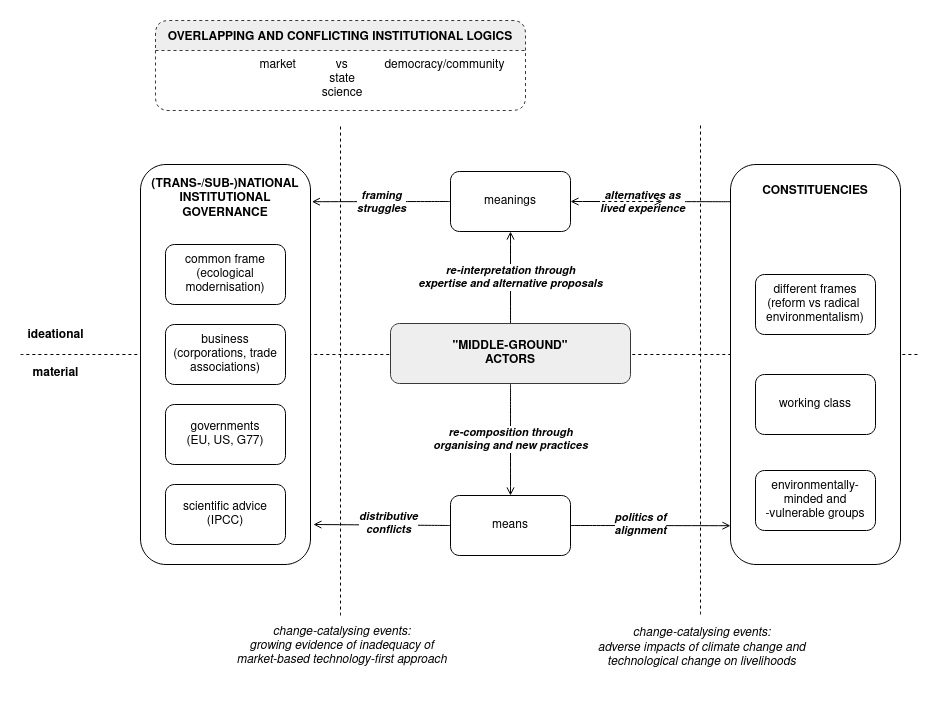
\includegraphics[width=1\linewidth]{./figures/middle_ground} \caption[The middle ground of strategic environmental agency]{The middle ground of strategic agency, situated between institutional governance and social constituencies on one axis and ideational and material negotiations and struggles on the other axis.}\label{fig:unnamed-chunk-4}
\end{figure}

\emph{I contend that the work of these organisations is future-oriented as they are contesting the present hegemonic context of climate action, whose potential adverse effects --- inadequate decarbonisation and unjust transition --- might assume their full relief only with time}. Their counterproposals will gain increased relevance and disruptive capacity if the \emph{change-catalysing events} such as climate-induced disasters come to pass, making the adverse effects of climate policies more evident to various social constituencies and the policymakers. However, to shift the framing of climate governance away from the market-driven technology-first strategies, a significant change in the entrenched positions of the dominant actors in that process is needed. Following the \emph{institutional logics} theory, such change can be achieved if the actors within the governance arena, combining in their organisational identity competing logics, move from the domination of one to the domination of another logic (\protect\hyperlink{ref-friedland_bringing_1991}{Friedland and Alford 1991, 256}; \protect\hyperlink{ref-thornton_institutional_2008}{Thornton and Ocasio 2008, 117}).\footnote{According to \protect\hyperlink{ref-friedland_bringing_1991}{Friedland and Alford} (\protect\hyperlink{ref-friedland_bringing_1991}{1991}), societies combine ensembles of institutional orders, each with its separate logic. The notion of institutional logic assumes that institutions are ``simultaneously material and ideal, systems of signs and symbols, rational and transrational\ldots{} supraorganisational patterns of human activity by which individuals and organisations produce and reproduce their material sub­sistence and organise time and space'' (\protect\hyperlink{ref-friedland_bringing_1991}{1991, 243}). Western societies combine institutional orders of state, capitalism, democracy, family, religion, and science. Organisations operate in fields structured by overlapping and competing institutional logics whose alternation can explain why organisations change their orientations, work with and against other organisations to instigate a change of their field and potentially societal structures. The institutional logics approach as a meta-theory of change is compatible with the strategic-relational approach in so far as the higher-level structures have their emerged logics, but they are enacted by actors to reproduce structures or to change them. Both meta-theories accentuate ideation, meaning, and culture as complementary to interest, means, and resources as the basis of social agency.} Currently, governments follow science, market, and bureaucratic logics, and to a far lesser degree a democratic logic --- this is particularly the case with the governments of the high-income countries that bank on technological and financial fixes to avoid distributive conflicts. But as distributive conflicts in their societies gain ground, they might come under increased pressure to include a democratic logic within the governance process. Similarly, if the technology-first transition continues not to deliver adequate and timely results, they might come under increased pressure to adopt stricter, higher-cost regulatory measures, acting against the market logic, to hasten mitigation and adaptation. These \emph{events} and \emph{shifting logics} might give ``middle-ground'' actors and their constituencies a greater shaping power over the future of climate policy. They might ``bring the society back'' into climate action (\protect\hyperlink{ref-friedland_bringing_1991}{Friedland and Alford 1991}).

If we return to the insights from the macro-social structural perspective, we cannot expect all strategies to be equally expedient and successful: under capitalism strategies demanding ``rapid, far-reaching and unprecedented changes in all aspects of society'' (\protect\hyperlink{ref-ipcc_global_2018}{IPCC 2018a}) have less institutional anchoring and resources than strategies that reproduce industrial-capitalist social relations and social metabolism. The existing relations nonetheless depend on the actors reproducing them prevailing over those challenging them. However, power is relational and defined by the interdependence of all segments of society. It aggregates both from the top but also from below. Institutional change depends on ongoing ideational and material negotiations and struggles that actors enter into with their different resources, the support they find in the selectivities of institutions through which they act, and the support of constituencies with which they work. As I suggested in the previous chapter, the change of framing is weakening the strong shaping and determinative capacity of the capitalist economy and the state over sociotechnical transition. Events that prise open the inadequacies of framing can therefore set off ``dislocations and articulations of overlapping or contiguous structures'' (\protect\hyperlink{ref-sewell_historical_1996}{Sewell 1996, 871}), \emph{allowing the proponents of alternative framings to impose them on the field and thus to transform the field.} Through the process of learning and the reflexivity in their actions, contesting actors can improve strategies that might catch on if the turn of events provides an opportunity --- thus destabilising and transforming the coherence of social structures that was attained through the reproduction of patterns of conduct (\protect\hyperlink{ref-jessop_economic_2012}{Jessop 2012, 51}). Obviously, an environmental organisation or a trade union operate in a structurally very constrained strategic space --- dependent on funding and contributions, dynamics of employment and unionisation, alliances with their constituencies and other groups, economic and political conjuncture. Yet even within that narrow operating space, they can fundamentally seize on a change-catalysing event to enter framing struggles with the alternative proposals they are developing over longer periods of time, just as they can seize that opportunity to re-align the material interests of the collectivities that they work with. How they might concretely articulate framing struggles and work to re-align the material interests of their constituencies toward an ecological transformation I will discuss over the following two chapters.

\hypertarget{middle-ground-organisations-as-epistemic-actors}{%
\section{``Middle-ground'' organisations as epistemic actors}\label{middle-ground-organisations-as-epistemic-actors}}

I have described the organisations I am engaging as not being scientific organisations. That is not entirely correct. While they are not bodies strictly tasked with conducting science, they have scientists and experts in their ranks studying the impacts, primarily social, of climate change. But more importantly, the science of climate change cannot be adequately circumscribed by placing it narrowly within the confines of the Earth system science or only within the remit of scientific institutions. A large part of research on climate change touches on social causation, sociometabolic processes, sociotechnical systems, social impacts, and social adaptation. As the scientific debates around the Anthropocene indicate (cf. \protect\hyperlink{ref-steffen_anthropocene_2011}{Steffen et al. 2011}; \protect\hyperlink{ref-latour_facing_2017}{Latour 2017}; \protect\hyperlink{ref-altvater_anthropocene_2016}{Altvater et al. 2016}; \protect\hyperlink{ref-edwards_vast_2010}{Edwards 2010}), social sciences can elucidate significant aspects of the interaction between society and nature, but also the ontological and epistemic assumptions of science, and its organisation as an institutionalised process of knowledge production (\protect\hyperlink{ref-merchant_death_1990}{Merchant 1990}; \protect\hyperlink{ref-barca_forces_2020}{Barca 2020}; \protect\hyperlink{ref-billi_what_2019}{Billi, Blanco, and Urquiza 2019}). Indicatively, the IPCC has three working groups: WG I focuses on the physical science basis, WG II focuses on impacts, adaptation, and vulnerability, and WG III focuses on mitigation, of which the latter two are clearly interdisciplinary and dependent on an analysis of social, economic, and political factors. We, therefore, need an expanded notion of where and how the science of climate change happens to give nuance to that co-implication of the scientific and the social. Specifically for the research contributions of the organisations I am engaging, I will qualify that co-implication through two concepts: ``post-normal science'' and ``situated knowledge.''

While the fundamental biophysical mechanisms of global warming and its anthropogenic causes are well understood, the dynamics of climate change at lower spatial or at longer time scales are understood with less certainty. To arrive at a greater degree of certainty will require a further deployment of ``knowledge infrastructures'' (\protect\hyperlink{ref-edwards_knowledge_2017}{Edwards 2017}), sophisticated research methods, computing technologies, additional funding, and institutional arrangements. This is the processual and institutional nature of scientific truth-finding. However, the institutional embeddedness of scientific processes makes such processes anything but socially neutral. They necessarily come with individual, organisational, and disciplinary priorities --- interests, values, and politics included. Such routine social loading of climate science qua science gets amplified once its findings are translated into political implications. Thus, climate policy prescriptions, as Bruno Latour (\protect\hyperlink{ref-latour_facing_2017}{2017, 25--26}) insists, cannot be disentangled from the description of climate facts and therefore scientists --- contra those climate sceptics and detractors who criticise them for not sticking only to facts --- should embrace the implication that all factual claims already come with political implications. Whether we date the origins of the Anthropocene back to the Neolithic Revolution 8000 years ago (\protect\hyperlink{ref-ruddiman_anthropocene_2013}{Ruddiman 2013}), to the colonial conquest around 1500 (\protect\hyperlink{ref-moore_capitalism_2015}{Moore 2015}), or to the beginnings of the industrial capitalism (\protect\hyperlink{ref-altvater_anthropocene_2016}{Altvater et al. 2016}) has very different political implications. Consequently, the IPCC, as a body tasked with producing assessments, not only explores the consequences of different scenarios, including those in which ``emphasis on economic growth shifts toward a broader emphasis on human well-being'' (\protect\hyperlink{ref-hausfather_explainer_2018}{Hausfather 2018}), but does not shy away from urging for ``rapid, far-reaching and unprecedented changes in all aspects of society.''

The philosophers of science Silvio Funtowicz and Jerome Ravitz have proposed to conceive the social loading of scientific problems where ``facts are uncertain, values in dispute, stakes high, and decisions urgent'' as ``post-normal science'' (\protect\hyperlink{ref-funtowicz_post-normal_2006}{Funtowicz and Ravetz 2006}; see also \protect\hyperlink{ref-funtowicz_post-normal_2001}{Funtowicz and Ravetz 2001}). Unlike the situations of normal science, in post-normal science the problems are defined by complex systems, the need to manage the uncertainties that emerge, and the conflictual social implications resulting from policy-making. For this reason, in post-normal science ``the problems are set, and the solutions evaluated, by the criteria of the broader communities that are affected'' (\protect\hyperlink{ref-funtowicz_quick_2021}{Funtowicz 2021}). Hence, problem-solving requires the inclusion of larger groups of stakeholders as an ``extended peer community'' that translates scientific findings into realities of the social world. All starting from their respective disciplinary positions and policy interests, their positions are equally legitimate.

Latour and Funtowicz and Ravitz have in mind the broad participation of different actors in the science and policy-making process. There is no single view on the complex whole of climate change and its implications, thus necessitating a dialogue (and struggle) ``among those who have an interest in the issue and a commitment to its solution'' (\protect\hyperlink{ref-funtowicz_post-normal_2006}{Funtowicz and Ravetz 2006}). However, due to the centrality of the global capitalist economy in the causation of climate change and the dependence of contemporary forms of life on the continued stability of that mode of production, the stakeholders (polluting corporations and governments, as well as different social groups) are negotiating their material interests beyond the clearly defined venues of policy-making. Behind-the-curtain lobbying and antagonisms spilling over from other socially-loaded issues interfere into the climate governance processes (\protect\hyperlink{ref-oreskes_merchants_2011}{Oreskes and Conway 2011}), particularly as distributive conflicts resulting from policy decisions are frequently shied away from in domestic policy contexts. \emph{This, I want to posit, is where the nexus of knowledge production and social organising in the messy and antagonistic ``middle ground'' attains relevance as political epistemology --- as a form of re-articulation of the ecological problem through the perspective of socially-grounded distributive conflicts unfolding largely outside of the representative policy-making arena.}

To specify how social situatedness and antagonism is relevant to scientific inquiry and expertise, a detour through the work of the feminist scholar of science Donna Haraway is helpful. Haraway sheds light on the relationship between the objectivity of science and the material politics of stakes, alignments, and antagonisms. In her seminal text on situated knowledge, Haraway is arguing against knowledge claims emanating as if from nowhere, positing that a partial, located, critical knowledge emerging from the embodied position of a knowing subject is a way to ground the ``radical historical contingency of knowledge claims'' in the ``faithful accounts of a `real' world'' (\protect\hyperlink{ref-haraway_situated_1988}{Haraway 1988, 579}). The appreciation of the partiality of knowledge she advocates does not renounce objectivity or rationality but rather makes them possible because it makes reflexively explicit the social life in which positions are grounded and to which they remain politically committed. This enables ``power-sensitive'' conversations between positions and thus truly rational --- i.e., socially reflexive --- knowledge claims.

Why is it so important that stakeholders reflect the materiality of their social world in political-epistemic processes? One of the main reasons why climate policies come up against significant obstacles when they meet social realities (as I will shortly discuss with the case of ``yellow vests'' protests) is that they tend to be reductivist and functionalist in their approach to the problems they aim to tackle: framing the climate problem as a primarily technical and financial fix in separation from its social consequences and reducing the many-sided ecological crisis only to the problem of CO2 emissions (\protect\hyperlink{ref-hoyer_seven_2010}{Høyer 2010}), resulting in measures that are targeted too narrowly to achieve only the desired deep-decarbonisation. However, emitting processes are baked into infrastructures, circuits of production and consumption, and patterns of everyday life. Carbon prices are imposed, hydrocarbons are made more expensive, buildings are retrofitted to be more energy-efficient, yet the decarbonising effects are frequently not deep and quick enough, they are met with indifference and inertia. \emph{The reason for that shortfall is that it is hard to exit from the existing carbon-intensive sociometabolic surround --- for as long as alternative infrastructures, patterns of social provision, and forms of consumption, and are not developed, encouraged, and made widely available in a coordinated manner.} The expansion of large-scale energy-intensive systems has transformed how technologies are embedded into the material infrastructures of everyday life. For instance, as modern heating systems developed, we have increased the number and the size of rooms we heat in a home while shedding added layers of clothing, resulting in a total transformation of not only technological systems but also patterns of behaviour whose effects cannot be easily unmade by insulation and energy price hikes (\protect\hyperlink{ref-shove_what_2018}{Shove 2018}). Similar examples highlighting private transport, throwaway technological objects, or the consumption of meat can be easily made.

\emph{Here the ``middle ground,'' with its politics of re-composing collective experiences, social practices, and lived reality, can directly challenge the reductivist fixes proposed by policymakers and push them to approach transformations in more material, embodied, and integrated ways.} For example, researchers affiliated with the IPE have studied energy poverty in the Croatian countryside only to conclude that the panacea prescribed by policymakers --- insulate the home, increase the energy efficiency, and lower the cost of energy --- fails to address the greater problem hiding behind energy poverty. Namely, the fact that it affects mostly older people that live in depopulated rural areas, where children have left family homes their parents built a long time ago in search of a better life or fleeing the war in the 1990s. To solve their energy poverty, these elderly people would be best served by relocation to care homes or collective housing arrangements somewhere where there is a greater density of population (\protect\hyperlink{ref-ancic_energetsko_2013}{Ančić et al. 2013}). Or, to give an example from Unite's work, by articulating demands for just transition, trade unions have been drawing attention to the fact that there might be fewer, less skilled, and more casualised jobs in the renewables sector compared to the fossil-fuel sector or at least that they might not be available in the same regions, so that a transition that is just cannot be simply the replacement of one form of energy generation with another, one industry with another, but has to alleviate social impacts through comprehensive social transformations. In this manner, the parallel work of expertise-building and of organising with the constituencies allows the ``middle-ground'' actors to work toward sustainability transitions that combine fossil-fuel divestment and low-carbon innovation with a strong build-out of social coalitions and new patterns of social reproduction, something that current instrumental and reductivist policies fail to do (\protect\hyperlink{ref-markard_sustainability_2012}{Markard, Raven, and Truffer 2012}; \protect\hyperlink{ref-rosenbloom_opinion_2020}{Rosenbloom et al. 2020}).

\hypertarget{the-shifting-tectonics-of-climate-politics}{%
\section{The shifting tectonics of climate politics}\label{the-shifting-tectonics-of-climate-politics}}

It has been almost 35 years since the climatologist James E. Hansen warned the US congress of anthropogenic climate change. It has been another 30 years since the UNFCCC signed in Rio came into effect. It has been a succession of years of mounting evidence of record temperatures, record ice melt, and record extreme weather events. And yet global annual emissions are not falling. The system of global governance, created through a string of treaties, hammered out in the tugs of war that were the conferences in Rio, Kyoto, and the ensuing Conferences of Parties (COP), particularly in Paris in 2015 where signees have committed to keep the global warming below 1.5°C --- that system of global governance has been struggling to produce the urgent action that is needed to stop the global warming. Only economic crises such as the 2008 great recession and the 2020 COVID-19 pandemic have made a serious dent in rising emissions. Arguably the most sophisticated international scientific advisory process the world has ever built, IPCC, and the impressive body of knowledge that it has synthesised since it was founded in 1988 provide proof that knowing does not translate easily into acting.

Over those 35 years, as the understanding of accelerating climate change and its observable impacts consolidated, the urgency of action in the view of the IPCC has increasingly come at odds with the meandering international governance processes. In the late 1980s, the consolidating liberal international order under the US hegemony, still benefitting from the Cold War's orientation toward science in the service of developmental state and arms race (\protect\hyperlink{ref-mazzucato_entrepreneurial_2013}{Mazzucato 2013}), placed trust in the advisory processes initiated by concerned scientists to help governments under the aegis of United Nations to steward the global climate commons. That liberal international order has, at the same time, through the structural adjustment programmes and the integration of the global free market, disembedded the free trade and capital flows from democratic control and popular participation (\protect\hyperlink{ref-polanyi_great_1944}{Polanyi 1944}), promising to create a global tide of economic growth that would lift all boats. However, the failure of neoliberalism to create a trickle-down economy to distribute the benefits of economic growth widely, the post-industrial impoverishment of former industrial communities, and the first big crisis of the neoliberal regime of accumulation in 2008 have destabilised that order and its hegemony. This crisis of 2008 has triggered a global wave of radical protests and occupations, but once the neoliberal political elites failed to respond and change the socioeconomic course, the destabilisation paved the way for illiberal, nativist, and anti-globalist political forces to ascend to power in democracies large and small, including the UK, the US, Brazil and Hungary. The anti-globalist turn had an immediate effect on global climate governance, with the US announcing its withdrawal from the Paris Agreement and Brazil reopening the Amazon for economic prospecting. The intergovernmental process threatened to devolve into what Wainright and Mann (\protect\hyperlink{ref-wainwright_climate_2018}{2018}) have called the chaos of ``Climate Behemoth,'' forcing individual governments and the EU to take the lead on climate action on their home turf. And while transnational governance has been restored in the meanwhile, its temporary devolution has brought to light that the domestic distributive conflicts --- struggles over who bears the cost of climate change and climate action --- might be a more significant factor in successful attempts to reduce emissions than the coordinated action of governments globally (cf. \protect\hyperlink{ref-mildenberger_carbon_2020}{Mildenberger 2020}).

To shed light on what has changed over the last three decades and the implications for the politics of translation of science into the lived realities of social constituencies, I want to claim that \emph{the disembedding of economic processes and their integration into the global capitalist economy that has unfolded under the liberal international order over the last four decades, has limited and undercut the capacity of societies to transform sociometabolic processes in a purposive fashion.} The shielding of the capitalist market, already written into the Rio Convention that explicitly limited any climate action from affecting international trade or growth (\protect\hyperlink{ref-unfccc_united_1992}{UNFCCC 1992}, Principle 12), has effectively made scientific findings calling for ``rapid, far-reaching and unprecedented changes in all aspects of society'' difficult to translate into policy that precludes ``far-reaching'' interventions into the operations of the market and the capitalist economy, the principle social driver of climate change. In fact, with the market-driven technology-first approach to the management of climate crisis, climate governance has embraced the neoliberal regime of accumulation premised on commodification and marketisation. Climate urgency can henceforth only be translated into incremental, flexible, least-cost actions. The implication is that there is no global governance process that would act on the precautionary principle to prevent the threat of climate disaster for the benefit of all, but rather a more fragmented, antagonistic, and messier political outlook where many are left fending for themselves --- within and across societies.

To glean what that messier political outlook looks like, it is instructive to recall the ``yellow vests'' protests, an eminently distributive conflict caused by climate action. In November 2018, the streets of France erupted as the neoliberal government of president Emmanuel Macron decided to introduce a carbon tax on petrol that should have financed the energy transition to renewables. It was a regressive consumer tax, introduced in the wake of tax breaks on assets and capital gains. The ``yellow vests'' movement spread quickly from the truck drivers to other constituencies of the \emph{peripheric} and working-class France, for whom the increases in the price of petrol had a significant impact on the cost of living, starting with the commute to work necessary to earn wages. Given the share of energy costs in their total household spending, the carbon tax would have been a financial burden five-time greater for lower- and middle-income working classes than for higher-income groups (\protect\hyperlink{ref-dinara_were_2018}{Dinara 2018}). Economic inequalities are tightly correlated with carbon inequalities. To demonstrate this, ahead of the Paris COP21 meeting, Lucas Chancel and Thomas Piketty (\protect\hyperlink{ref-piketty_carbon_2015}{2015}) have published a study on emissions and inequality, concluding that inequalities in per-capita emissions between societies are significant (an average US citizen in 2013 emitted 22.5 tCO2e/year --- compared to the global average of 6.2 tCO2e/year), but inequalities within societies are staggering (upper 1\% of US emitters releases on average a whopping 318.3 tCO2e/year, hundred times the world's average). Globally, the upper 10\% emits 45\%, the next 40\% emits 42\%, while the remaining 50\% emits 13\% of all emissions. In fact, the inequalities of emissions are roughly following the same distribution pattern as inequalities of income. Yet, the costs of living are only a small proportion of costs for high-income groups, who can also easily avoid ecological taxes by buying less-polluting technologies.

Climate change comes with a price tag --- according to the 2007 Stern report, the non-action would reduce the global GDP by around 20\%, whereas immediate action would require as much as 1\% on a yearly basis (\protect\hyperlink{ref-stern_economics_2007}{Stern 2007}). Fifteen years of growing emissions later, a McKinsey report puts the yearly number to reach net-zero by 2050 at a more substantive 7.5\% (\protect\hyperlink{ref-mckinsey_net-zero_2022}{McKinsey 2022}). These are obviously investments, not only costs. \emph{Still, the mitigation to drive down emissions and the adaptation to heatwaves, wildfires, droughts, floods, sea-level rise, higher food prices will have a cost that someone will have to pay in money, but in the absence of significant redistribution and precautionary action in health and lives as well}. Just as someone has had to pay for the neoliberal restructuring in industrial economies since the late 1970s (\protect\hyperlink{ref-louis_who_2019}{Louis 2019}). For many in the streets of France that price tag has a long time ago become part of the everyday. They have learned to calculate the cost of restructuring, lower wages, casualisation, and the reduction of public services. They have witnessed the upward redistribution of social wealth. For them, the transition in response to climate change, as proposed by the Macron government, was recognisably a continuation of that neoliberalisation process. Metaphorically, they have already borne the burden of climate change.

The last forty years of neoliberal restructuring are the legacy of the same international liberal order that is willing but potentially unable to act on climate change by striking there where the pollution reduction to accelerate and the money to finance the transition can be found. The globalisation of capital flows and the concerns over energy security have made it impossible to tax around 100 carbon majors that are responsible for 63\% of all historical emissions and 71\% of all emissions since 1988 (\protect\hyperlink{ref-heede_tracing_2014}{Heede 2014}; \protect\hyperlink{ref-griffin_carbon_2017}{Griffin 2017}). The shielding of capital from these kinds of interventions is the outcome of the project of neoliberal globalists (\protect\hyperlink{ref-slobodian_globalists_2018}{Slobodian 2018}), who have constructed an international institutional and legal order that has effectively put the command over capital largely out of reach of democratic law-making. While they have institutionally secured the smooth operation of the global capitalist economy, they have made it impossible to intervene in a substantive way in the operation of that economic system. All global crises now have to be overcome through the conditions set by that system. As the anthropologist Joseph Masco has formulated in his discussion of the changing political valence of the notion of crisis, instead of ``the crisis-utopia circuit that empowered the high modernist culture of the mid-twentieth century, we now have a crisis-paralysis circuit'' (\protect\hyperlink{ref-masco_crisis_2017}{Masco 2017, 66}). \emph{With the eclipse of socialist, developmentalist, and post-colonial projects, ``futurity'' as a horizon of positive social transformation has been increasingly removed from the dominant political discourse, and the crisis narrative serves primarily to amplify the sense of danger that the state is called onto to resolve by ensuring the stability and the continuation of the status quo.} The catastrophist discourse of climate change, as Erik Swyngedouw has been warning (\protect\hyperlink{ref-swyngedouw_apocalypse_2013}{2013, 10}), serves to drown out the antagonisms that hide behind the promise of technocratic governance to manage the crisis and to effectively de-politicise conflicts such as the one that has surfaced with the ``yellow vests'' movement in France.

Where do the stumbling attempts of the (trans/sub)national climate governance process to take decisive action and the receding sense that climate change can be cautiously steered for the benefit of all leave the ``middle ground'' then?\footnote{The gap between the ambition and the results is on display from COP meeting to COP meeting, well condensed in the UN Secretary-General Guterres's COP26 concluding statement: ``unfortunately the collective political will was not enough to overcome some deep contradictions'' (\protect\hyperlink{ref-guterres_secretary-generals_2021}{Guterres 2021}).} Wither with its materialist politics of knowledge production? First, I would propose to view that predicament as an opening of a horizon rather than a closing. The material interests and values of various segments of societies --- their implicit environmentalisms --- will continue to bubble up as the impacts of climate change become more pronounced and policies are hurried to address them in a more targeted fashion. The experience of unjust burden for the French lower- and middle-income working classes bears a direct link to their vulnerability in the process of inchoate mitigation and adaptation to the impacts of climate change (see section 7.2.2). ``Yellow vests'' protests did manage, with the help of climate activists, to articulate their discontent in terms of demands for urgent climate action and just transition. \emph{In such experiential openings, ``middle-ground'' organising will be able to lead on re-articulating and re-arranging the interests of diverse social constituencies.} Developing a just and sustainable transition through the participation of these constituencies is harder than imposing top-down sustainability measures. However, those demonstrably cannot be imposed on popular masses expecting that they will ``pick up the bill.'' Achieving a just and sustainable transition will entail something that the philosopher of science Isabel Stengers (\protect\hyperlink{ref-stengers_catastrophic_2015}{2015}) has called the acts of composition, wherein the experiential and situated knowledge of heterogeneous groups are brought together and made to matter in equal ways, rather than being suppressed as they are in the reductive approach of technocratic governance that abides only by the imperatives of carbon reduction and economic growth --- so that, in Stengers's view, we can preserve a chance for a future that is not barbaric. In her account of the enclosure of the commons, Stengers highlights the notion of a common that is inherent to a group --- of the knowledge that makes that group ``think, imagine, cooperate'' (\protect\hyperlink{ref-stengers_catastrophic_2015}{2015, 85}). Therefore, situated knowledges should be seen as the key to survival. The actors in the ``middle ground,'' I would argue, are in a privileged position to develop that knowledge with their social constituencies starting from the existing social experience and adapt the existing social practices to the destabilisation that arrives with growing imapacts of climate change.\footnote{Stengers warns that the threat that a community's world might end, implicit in the destruction of their ecosystems, is not an altogether new experience. For some, it is a continuation (for those who have the collective experience of colonialism, imperialism, or neoliberalism) or a repetition (such as for Amerindians, who have already survived the end of their world once with the arrival of the conquistadors, cf. \protect\hyperlink{ref-danowski_ends_2016}{Danowski and Viveiros de Castro 2016}).}

\hypertarget{capitalist-cosmology-and-ecological-rationality}{%
\section{Capitalist cosmology and ecological rationality}\label{capitalist-cosmology-and-ecological-rationality}}

To conclude this chapter, I will step away from the entanglements of political epistemology and distributive conflicts in the context of (trans)national climate governance to broaden the perspective. I want to briefly consider how can efforts to construct sustainable ways of living and knowing in societies inside and societies outside of the capitalist world-system of states be read together from the shared planetary ecology. In a plurality of diverging ways of living and their implicit or explicit cosmologies, what is the relevance of struggles against the present industrial-capitalist social metabolism for those who are outside of it and what is the common ground on which to judge the ecological viability of any particular cosmology and social metabolism?

According to the World Bank, around 55\% of the global population lives in urban zones, necessarily depending on formal or informal wages to secure significant parts of their subsistence. As part of the 45\% of the world's population living outside of urban areas, particularly throughout the territories of Latin America, Africa, Asia and Pacific islands, there are sizeable rural and indigenous populations that still live in subsistence economies. Few of them are, though, untouched by the capitalist exchange economy. A significant part of the global population lives, in fact, in various forms of dual economy --- and elements of their local economies are integrated into the global commodity flows (\protect\hyperlink{ref-tsing_friction_2005}{Tsing 2005}). Hence, the large majority of the global population lives, to some degree, in capitalist relations. However, if the capitalist system would conceivably allow for all of the world's population to advance to the status of affluent nations, appropriating an equal share of the bioregenerative capacities of the planet, the Earth's subsystems that cannot sustain the present level of appropriation would be irrecuperably destabilised. The question of changing the course of capitalist development affects thus all of the global population directly, even those who remain largely unaffected by it. This begs the question of how to preserve the diversity of existing and construct the diversity of future ways of living --- starting from the societies entrenched in capitalism, but also of how to assess these existing and future ways of living from the point of their local and planetary environmental sustainability and reproduction --- and abolish those that are unsustainable.

I want to propose that there is a common ground to compare any cosmology --- capitalist-instrumental, ecosystemic such as Buen Vivir, or various indigenous biocentric cosmologies (see \protect\hyperlink{ref-kothari_pluriverse_2019}{Kothari et al. 2019}; \protect\hyperlink{ref-danowski_ends_2016}{Danowski and Viveiros de Castro 2016}), to the degree that, ultimately, it is an account of a society's metabolic exchanges with the environment it inhabits and, thus, an expression of its ecological rationality (this notion is also developed in a slightly different way by \protect\hyperlink{ref-dryzek_ecological_1983}{Dryzek 1983}). \emph{If a cosmology is able to conceive of and sustain in practice the dependence of its way of living on the stable variability and regeneration of its environment, taking into account both its direct and indirect impacts, it can be judged as ecologically rational}. Judged on that common rational ground, capitalist cosmology fails miserably, destabilising not only its immediate environment, but a shared planetary.

It is thus not surprising that indigenous populations --- the Zapatistas for instance --- are frequently some of the most militant champions of abolition of both capitalist cosmology and its way of living. The acts of composition that are the key to survival have to be not only acts of composition and allying with but also composition and allying against --- acts of negation and abolition. In \emph{Facing Gaia} Bruno Latour (\protect\hyperlink{ref-latour_facing_2017}{2017}, Eighth lecture) elevates this antagonism to no less than a Schmittian notion of war between those who uphold the separation Culture/Nature and those who are reassembling the severed bonds across that dichotomy. Different redistributions of agency, or ``cosmograms,'' are then convoked by Latour's vision into a diplomatic assembly of the peoples struggling for the Earth and representing their own territories. Leaving aside the discussion of the Culture/Nature separation, one only needs to read Phil Neel's account of the US \emph{Hinterland} (\protect\hyperlink{ref-neel_hinterland_2018}{2018}) to get a sense of how conservative political forces antagonistic to a plural understanding of the world are also \emph{composing with} for their own survival and \emph{mobilising against} those who are challenging systemic forms of gender, race, and class privilege. It is not surprising that there are many forms of composing with. What is surprising is to think that those forms of composing with would not be overcoded by the structuring social antagonisms of capitalist nation-states. This is the problem Latour faces: we cannot avoid having our skin in the game where capitalist nation-states are calling the shots. Their market-driven technology-first response to climate destabilisation is a threat to all societies.

The conflictual nature of politics in the present makes Latour's preference for a representative assembly in which all positions --- in equal measure those of nations and peoples, of modern artefacts, and of non-human actors such as oceans, but probably of polluting industries as well --- are brought around the same table and expected to negotiate their interests in full disclosure seem like a deep-ecologist version of liberal republicanism (for his notion of the {``Parliament of Things''} see \protect\hyperlink{ref-latour_we_1993}{Latour 1993a, 142ff}; \protect\hyperlink{ref-latour_realpolitik_2005}{2005}). Politics takes many forms, of which diplomatic summits and representative assemblies are only a part, but also in protests, acts of sabotage, migrations, strikes, epistemic clashes, lobbying, money in politics, all that nitty-gritty of political subjectivation and conflict that does not readily enter a parliamentary frame of analysis. \emph{To compose with, one always needs also to compose against.} No matter how we conceive the work of composition, the hard political truth of the matter is that fossil capitalism, if it continues on its present course, will keep spouting emissions until the climate system is locked into a spiral leading to a planetary condition too hot to have any living agency to compose with across many places of the world. The implication is that there is no political way around antagonisms. Acting in alliances between societies and cosmologies on parallel fronts of climate science, climate policy, the composition of different ways of living and knowing, as well as on the disruption of polluting technology systems, their legitimational underpinnings, and inadequate technology-first strategies are all part of the political task of enabling different livable futures, for both the humanity that lives inside and the humanity that lives outside of the ``capitalist condition.''

In the next two chapters I will delve only into a small slice of those endeavours aimed at re-politicising environmental action --- situated in the middle ground, antagonising on the institutional terrain, and composing with on the social terrain.

\hypertarget{degrowth-environmentalism-modelling-safe-and-just-futures-from-the-semiperiphery}{%
\chapter{Degrowth environmentalism --- modelling safe and just futures from the semiperiphery}\label{degrowth-environmentalism-modelling-safe-and-just-futures-from-the-semiperiphery}}

\minitoc

\hypertarget{introduction-from-framework-to-fieldwork}{%
\section{Introduction: from framework to fieldwork}\label{introduction-from-framework-to-fieldwork}}

Over the previous three chapters, I have conceptualised, historically and theoretically, the strategic agency of organisations operating in the ``middle ground,'' situated between the institutional ensembles of the capitalist state and the social constituencies with their ideationally and materially structured social worlds. My objective was to create frameworks that would tease out the structural and conjunctural circumstances that enable these organisations to disrupt the dominant market-driven technology-first approach in global environmental governance.

To arrive there, in chapter 3, I have provided a historical evolution, through class struggle and technological change, of industrial-capitalist social metabolism, characterised by a growing appropriation of resources from nature and labour from the (neo)imperial global geography propelled by fossil fuels. I have highlighted this metabolism's post-WWII consolidation into an economy of growth and wasteful energy systems, subject to transnational governance and militarised geopolitics. In chapter 4, I have proceeded to argue that that social metabolism is organised through large-scale interlocking technological systems and that their attained size constrains --- through technical, biophysical, energetic, and economic lock-ins --- attempts to transform it. The strategic capacity of social actors aiming to do so is additionally constrained by the actions of other, more powerful social forces through the structures of the state and the capitalist economy. In such technologically and institutionally constrained terrain, the transnational governance process around the UNFCCC has adopted an ecological modernisation framing to mitigate climate change. With the uncertainties of goal-oriented transition aimed at unprecedentedly rapid decarbonisation, the strong influence of the state and the capitalist economy over the direction of transition has weakened, opening up a strategic terrain to contest the technology-first approach in environmental governance. Finally, in chapter 5, I have analysed why such an incremental, flexible, least-cost technology-first approach is resulting in a transition that is failing to keep the global warming down to 1.5°C or 2°C above the pre-industrial levels. This generates a unique opportunity for the ``middle-ground'' actors to articulate alternative pathways and develop social practices that would allow societies to steer the transition toward ecologically sustainable and socially just futures for all.

Over the next two chapters, I will report and reflect on my fieldwork with two such actors --- an environmental organisation in Croatia and an industrial trade union in the UK. The fieldwork was conducted so as to provide concretised answers to what do these organisations concretely do to contest the presently dominant technology-first approach, what are the alternatives they propose to displace it, how they engage their social constituencies to translate these proposals into their lived experience, and what prospects do their proposals open up to in the current conjuncture.

In this chapter, I will engage with IPE and degrowth environmentalism. \emph{I will contend that degrowth environmentalism is the most comprehensive and disruptive attempt at re-framing environmental action because it inverts the terms under which sustainability transition is conceived.} It posits that an environmentally safe --- but also socially just --- transition can be more adequately and timely achieved by delinking the transition from the imperative of economic growth and a reduced focus on technological restructuring. If the growing demand for energy and materials in affluent societies is throttled down through a democratic transformation of the patterns of production and consumption on the principles of private sufficiency and public abundance, the deployment of green technologies does not need to scale at such a historically unprecedented rate, while the fossil fuels can be phased out more expediently. \emph{As it is significantly focused on framing struggles, degrowth environmentalism places a particular focus on research and expertise.} It draws on a rigorous and non-reductivist scientific understanding of the environmental crisis, models alternative epistemic tools, studies intra- and inter-societal inequities, and articulates integrative North-South perspectives. Beyond these epistemic endeavours, degrowth as a movement also develops and disseminates future-oriented, prefigurative proposals of resilient provision for social needs.

I focalise the account of degrowth around IPE as an important nodal point in the international degrowth movement. I have selected IPE as my case study for four principal reasons:

Firstly, I share research and activist contexts with IPE. As explained in the Introduction in greater detail, from 2013 on I have been involved in the debates organised by the Zagreb-based green-left think-tank Grupa22 (\protect\hyperlink{ref-grupa_22_us_2018}{2018}) that have led to the founding of IPE in 2015 and ever since I have been an external participant in the educational, research, and advocacy activities that IPE has been organising --- first and foremost through its biannual Green Academy (\protect\hyperlink{ref-ipe_green_}{IPE n.d.b}) and its involvement in the international Degrowth Conferences. In those exchanges with IPE, I have primarily scrutinised degrowth's approach to technologies (\protect\hyperlink{ref-medak_technologies_2018}{Medak 2018}). This research is a continuation of that dialogue.

Secondly, IPE is closely connected with the most prominent environmental and spatial justice organisations across Croatia and the neighbouring countries, such as Zelena Akcija/Friends of the Earth Croatia, Pravo na grad from Zagreb, and Ne davimo Beograd from Belgrade, but also with local communities developing sustainability solutions. Beyond the work with these communities and intermediaries, it is involved in institutional framing struggles with its team members participating of the IPCC review processes and a variety of consultation processes in Croatia around climate and environment protection policies, public services, and the commons.

Thirdly, IPE is based in Croatia, a post-socialist, semiperipheral EU country, providing a political and social context that does not fit neatly into the dominant Global North/Global South divide into which environmentalisms are typically separated out, and thus offers its own specific entry-point into degrowth debates.

Fourthly, IPE shares several of its affiliated and core members with the two emerging political platforms of the green-left in Croatia: the municipalist platform Zagreb is Ours! and the national platform Možemo! In fact, since I conducted my fieldwork, its former research co-lead, Tomislav Tomašević, has become a parliamentarian and then the mayor of Zagreb. This close link to municipal politics provides, as the other IPE's research co-lead has highlighted in the interview, a short iterative feedback loop between IPE's environmentalist vision and the political reality it addresses. As it operates in a small political context, the success of these platforms can significantly shift the Overton window of accepted debate on environmental crisis and strategies of addressing it.

I have conducted my fieldwork with IPE over the course of 2019, working primarily with the organisation's research team. The principal methods I have used in preparing and conducting the fieldwork were analysis of primary and secondary documents, participant observation, and semi-structured interviews. In addition, the fundamental positionality of my fieldwork was to contribute with my research to their work on producing research, building expertise, and disseminating knowledge and practices to their own constituencies. That co-research consisted of the following:

\begin{itemize}
\tightlist
\item
  assisting in the development of the Degrowth Doughnut model tool (\protect\hyperlink{ref-ipe_degrowth_2019}{IPE 2019}), which is discussed below in section 6.4;
\item
  lead-authoring an article on ``Degrowth'' for the \emph{Encyclopedia of the World's Biomes} (\protect\hyperlink{ref-medak_degrowth_2020}{Medak, Domazet, and Rilović 2020}), which constitutes a part of sections 6.2 and 6.5 (without contributions by my co-authors Mladen Domazet and Andro Rilović);
\item
  contributing in a minor role to an article on ``The Degrowth Doughnut Model'' for the same \emph{Encyclopedia} (\protect\hyperlink{ref-domazet_mental_2020}{Domazet et al. 2020b});
\item
  presenting a paper in the 2019 Historical Materialism conference on ``Degrowth - Developing a Future-Oriented Vision of Social Wellbeing within Planetary Biophysical Boundaries.''\footnote{In the spirit of collaboration, I have also assisted in other activities of IPE throughout that year, which did not directly contribute to my research, such as translating texts for their website, giving presentations on technology and ecology in their academic and public outreach programmes, or contributing in the programme of their Green Academy.}
\end{itemize}

By drawing on that fieldwork, I will analyse how in its specific inflexion through the work of IPE, situated in the context of a post-socialist society, degrowth environmentalism (section 6.2) suggests that a systemic change resulting in private sufficiency and public abundance might be acceptable to broad segments of the population --- assuming a radical redistribution of social wealth that distributive conflicts over future climate action might call for. And in the context of a semiperipheral economy, one that struggles to embed itself into the global capitalist economy, IPE's approach to degrowth suggests that the democratic downscaling and transformation of polluting patterns of production might be more easily achieved if it is developed and spread from a local and municipal level (section 6.3). Provided there are tools such as IPE's Degrowth Doughnut (section 6.4), facilitating a multiscalar understanding of how to reckon with social and biological shortfalls and transgressions, such a transition can also be institutionally governed. It might lead us out of the unsustainable 20th-century developmental trajectory onto a pathway of the mutual flourishing of society and nature, thus presenting a strong framing alternative to the technology-first approach. Lastly, I will discuss some aspects of degrowth critically and, by way of conclusion, analyse its future-oriented, prefigurative experimental proposals as acts of speculative and prefigurative construction for a ``rejective future'' in a ``full world'' (section 6.5).

\hypertarget{understanding-degrowth-environmentalism}{%
\section{Understanding degrowth environmentalism}\label{understanding-degrowth-environmentalism}}

\hypertarget{origins-of-degrowth}{%
\subsection{Origins of degrowth}\label{origins-of-degrowth}}

Degrowth is a social movement and a research framework advocating a transition to forms of social organisation that are sustainable and just. It proposes to achieve this double objective by ``de-growing'' the energy and matter throughput of the global economic system and re-orienting economic activity centred on resource-intensive production toward socialised provisioning for human wellbeing (\protect\hyperlink{ref-kallis_degrowth_2018}{Kallis 2018}). As a ``transitional discourse'' envisioning alternative societies built on ``ecological integrity and social justice'' (\protect\hyperlink{ref-escobar_degrowth_2015}{Escobar 2015, 1}), it approaches the transition from a systems-thinking perspective that combines the values of ecology, justice, wellbeing, and democracy (\protect\hyperlink{ref-demaria_what_2013}{Demaria et al. 2013}) with a theoretical grounding in Earth system science, ecological economics, political ecology, and post-development.

Degrowth emerged in the early 2000s out of the earlier environmental movements from dissatisfaction with the transnational governance of the planetary ecological crisis. Since at least the Kyoto Protocol, this process has explicitly wedded the action of governments to the commitment to economic growth and technological innovation, although these two pillars of the capitalist system of production have driven a growing appropriation of energy and matter and the degradation of the ecosystems across the planet. The contemporary degrowth movement includes three aspects: theoretical, activist, and political. These are loosely integrated through a continuous exchange in international degrowth conferences, scholarly publishing, and interaction with other environmental and social justice movements (\protect\hyperlink{ref-martinez-alier_sustainable_2010}{Martinez-Alier et al. 2010}). Unlike the ideas of sustainable development, green growth, and green capitalism, degrowth insists that environmental stability and sustainability can only be achieved through a departure from the present growth-oriented global capitalist system.

The term draws its inspiration from \emph{The Limits to Growth} report to the Club of Rome published in 1971. It was first coined as ``décroissance'' by French-German philosopher and political ecologist André Gorz in a debate a year later. The word ``officially'' entered into English with the first Degrowth Conference held in Paris in 2008 (\protect\hyperlink{ref-demaria_what_2013}{Demaria et al. 2013}: 195). Initially, the idea of \emph{décroissance} rallied together the grassroots activists working on issues such as environmental justice, protection of the environment, or opposition to extractivism with the practitioners of alternative forms of organisation of social production and reproduction like permaculture, cooperatives, ethical banks, co-housing, squatting, and recycling, gradually consolidating into an international social movement (\protect\hyperlink{ref-demaria_what_2013}{Demaria et al. 2013, 202--3}). Regular international conferences crystallised degrowth also as an activist-led research agenda (\protect\hyperlink{ref-martinez-alier_science_2011}{Martinez-Alier et al. 2011}) and a platform for political advocacy. The research agenda received its provisional manifesto in the lexicon \emph{Degrowth: A Vocabulary for a New Era} (\protect\hyperlink{ref-dalisa_degrowth_2014}{2014}), whereas the political advocacy had its first international high-profile foray with the Post-Growth Conference held at the European Parliament in 2018.

\hypertarget{endless-growth-on-a-finite-planet}{%
\subsection{Endless growth on a finite planet}\label{endless-growth-on-a-finite-planet}}

The foundational insight for degrowth is that there cannot be endless growth on a finite planet. While the Earth is not an entirely closed-off system, almost no matter enters the atmosphere, and the incoming solar energy is not readily convertible into work. Thus the regeneration of energy stocks and the recycling of matter available for human use can unfold at a very slow rate.

However, the pattern of continuous economic growth inaugurated by capitalism ignores the limits of planetary stocks and flows. Over the last century, global material extraction and primary energy consumption have grown roughly tenfold to 90Gt/year (\protect\hyperlink{ref-irp_global_2018}{IRP 2018}) and 525eJ/year (\protect\hyperlink{ref-smil_energy_2016}{Smil 2016, 241}). The world's ecological footprint currently exceeds the annual bioregenerative capacity of the planet by 70\% (\protect\hyperlink{ref-global_footprint_network_earth_2021}{Global Footprint Network 2021}). Human use has significantly altered 75\% of global ice-free land (\protect\hyperlink{ref-ellis_putting_2008}{Ellis and Ramankutty 2008}) and 66\% of marine environments (\protect\hyperlink{ref-ipbes_global_2019}{IPBES 2019}) and appropriates around one-third of the net primary production of terrestrial systems (\protect\hyperlink{ref-haberl_human_2014}{Haberl, Erb, and Krausmann 2014}).

This expanding dynamic of extraction has led to a number of negative impacts on Earth's biophysical systems, pushing them beyond their Holocenic variability during the previous 10.000 years that provided a safe operating space for human societies to thrive (\protect\hyperlink{ref-rockstrom_planetary_2009}{Rockström et al. 2009}). The effects of these disruptions are unevenly distributed, impacting the most economically (\protect\hyperlink{ref-diffenbaugh_global_2019}{Diffenbaugh and Burke 2019}) and environmentally disadvantaged communities hardest. At present, no country stays within its ``fairly apportioned global biophysical boundaries'' while meeting the social needs of its people (\protect\hyperlink{ref-oneill_good_2018}{D. W. O'Neill et al. 2018}). From a degrowth viewpoint, in order to bring societies within the planetary boundaries, the pattern of expanding extraction has to be reversed, and the provisioning systems addressing societal needs must be organised differently.

The patterns of resource use change throughout history as the modes of production and the modes of social and ecological reproduction come into contradiction (\protect\hyperlink{ref-merchant_theoretical_1987}{Merchant 1987}). These patterns define sociometabolic regimes (\protect\hyperlink{ref-fischer-kowalski_sociometabolic_2014}{Fischer-Kowalski, Krausmann, and Pallua 2014}). Under the fossil-fuelled industrial capitalism, the surplus produced by the workers is appropriated by the owners of capital for private consumption and, fundamental to sustaining the dynamic of growth, for reinvestment into the further accumulation of capital. The process of capital accumulation under the conditions of competition sets an imperative to raise productivity, resulting in growing economic output, i.e., an ever-greater quantity of goods or services produced in a given period of time. As \emph{Figure 4.1} indicates, this growing economy has a strong historical correlation with the increase of material extraction and CO2 emissions (1\% increase in GDP resulting in 0.6\% increase of material footprint (\protect\hyperlink{ref-wiedmann_material_2015}{Wiedmann et al. 2015}) and 0.5-0.8\% increase in emissions (\protect\hyperlink{ref-burke_carbon_2015}{Burke, Shahiduzzaman, and Stern 2015})). The capitalist mode of production thus destabilises the processes of ecological reproduction.

Economic growth at the national level is measured in GDP. Economic policies are drawn up to keep the GDP growing year on year, and GDP growth is a key performance indicator upon which governments stand or fall. The healthy annual growth rate of an advanced economy is considered to be between 2\% and 3\%, leading to a doubling of economic activity roughly every 24 to 35 years. The drivers behind this expectation of growth are twofold. On the side of system reproduction, capital is borrowed with the expectation that future growth will repay the debt and interest that, in the next step, serve as capital for future borrowing. On the side of system justification, the competitive forces of the market tend to reduce wages and create inequalities, whereas growth allows policymakers to promise an increase in wages in the future without needing to redistribute the existing social wealth in the present.

However, researchers on the subject of inequality have documented that in middle- and high-income countries the expected trickle-down effect of wealth has not happened since the late 1970s: as growth in wealth and income has concentrated at the top, the wages of the working class have largely stagnated (\protect\hyperlink{ref-piketty_capital_2014}{Piketty 2014}; \protect\hyperlink{ref-milanovic_global_2016}{Milanović 2016}; \protect\hyperlink{ref-hickel_divide_2018}{Hickel 2018}). For instance, over the same period in the US the wages of the upper 1\% have risen by 160\%, whereas the bottom 90\% have seen a modest increase of 26\% (\protect\hyperlink{ref-epi_wages_2020}{EPI 2020}). Elsewhere around the world, in the decade 1999-2008, the poorest 60\% has received only 5\% of the global growth (\protect\hyperlink{ref-woodward_incrementum_2015}{Woodward 2015}). Even with the exceptional effect that the reduction of absolute poverty in China has had, relative poverty in the world has increased since the 1980s (\protect\hyperlink{ref-chen_policy_2012}{Chen and Ravallion 2012}). Alternative indicators of social progress like the Genuine Progress Indicator (\protect\hyperlink{ref-anielski_genuine_2002}{Anielski and Sosklone 2002}) reveal that once the negative social and environmental impacts are accounted for, growth beyond a certain level does not bring an increase in objective and subjective wellbeing and is environmentally disastrous (\protect\hyperlink{ref-kallis_degrowth_2018}{Kallis 2018}, ch.~4).

While the dominant policy approach assumes that growth can be maintained while making economic processes green, empirically there is sparse evidence that a significant reduction in greenhouse gase emissions and material extraction can be achieved for a sustainably long period of time on a global scale while maintaining growth (\protect\hyperlink{ref-hickel_green_2019}{Hickel and Kallis 2019}). The hope is that the accelerated deployment of renewables, carbon drawdown, and carbon cap-and-trade schemes might change that in the future. Indeed, a few countries have recently seen an absolute decoupling, with emissions falling while the economy kept growing (\protect\hyperlink{ref-quere_drivers_2019}{Quéré et al. 2019}). However, their observed annual decoupling of less than 1\% is far from the annual rates of 14\% required to achieve net-zero by 2050 (\protect\hyperlink{ref-jackson_unraveling_2019}{Jackson and Victor 2019}). But beyond that small group, environmental policies have so far only been able to achieve relative decoupling, with emissions just rising at a slower rate than the economy (\protect\hyperlink{ref-haberl_systematic_2020}{Haberl et al. 2020, 34}). In fact, the decoupling of growth from the growing energy demand and material extraction might not be achievable at all (\protect\hyperlink{ref-ward_decoupling_2016}{Ward et al. 2016}; \protect\hyperlink{ref-parrique_decoupling_2019}{Parrique et al. 2019}). This suggests that if the IPCC's warnings of a runaway climate change (\protect\hyperlink{ref-ipcc_global_2018}{IPCC 2018a}) and IPBES's warnings of an unprecedented loss of natural life (\protect\hyperlink{ref-ipbes_global_2019}{IPBES 2019}) are to be taken seriously, human action faces a difficult choice between rapid reduction in throughput or the potential collapses of ecosystems. Facing this choice, degrowth offers diagnoses and strategies (\protect\hyperlink{ref-demaria_what_2013}{Demaria et al. 2013, 194}) that address major obstacles to transformations that are needed to make global social metabolism sustainable --- i.e., how to prevent that the rapid reduction in throughput leads to a reduction in social wellbeing.

\hypertarget{degrowth-economics-bringing-the-economy-back-into-the-biosphere}{%
\subsection{Degrowth economics: bringing the economy back into the biosphere}\label{degrowth-economics-bringing-the-economy-back-into-the-biosphere}}

Degrowth is in principle agnostic as to whether the planned reduction of throughput will lead to a reduction in economic output. Degrowth's goal is certainly not economic depression but long-term sustainability and societal wellbeing. However, the reduction in greenhouse gases needed to stay within the Paris Agreement goals is likely achievable only if the world economy throttles down the present patterns of growth driving the increasing use of polluting energy and extraction. The world would have to cut net emissions to zero by 2050 in order to have a 50\% chance of staying under 1.5°C or by 2070 to stay under 2°C (\protect\hyperlink{ref-ipcc_global_2018}{IPCC 2018a}). The degrowth scholars Jason Hickel and Giorgos Kallis have calculated that the necessary annual reductions in emissions to achieve those targets at a zero growth rate would have to be 6.8\% and 4\% respectively, but at a 2\% growth rate they would have to be as high as 8.8\% and 6\% (\protect\hyperlink{ref-hickel_green_2019}{Hickel and Kallis 2019}: 15). For comparison, in the pandemic lockdown year 2020, the emissions fell by 6.4\% (\protect\hyperlink{ref-tollefson_covid_2021}{Tollefson 2021}). However, those 6.8\% and 4\% are equal to or above the most optimistic predictions that put emission reductions at a maximum 4\% annually --- implying that the target of staying under 2°C might be achievable, but only with a rapid deployment of deep decarbonisation strategies (transition to 100\% renewables, afforestation and soil regeneration, and shift to alternative production processes) and, crucially, at a zero growth rate (\protect\hyperlink{ref-hickel_green_2019}{Hickel and Kallis 2019, 15}).

The objective of growth is thus at odds with the biophysical realities of climate change mitigation. It is for this reason that degrowth has taken up the task of challenging the economic orthodoxy that underpins climate change policies. This undertaking necessitates that degrowth mounts a critique not only of growth but also of the economic science for which it is axiomatic. \emph{The critique of conventional economics is the cornerstone of degrowth's epistemic agency.} The economic field is dominated by formal economic analysis focusing on markets and prices while disregarding substantive determinants of economic processes in metabolic interactions between society and nature and the societal purposes of economic processes (\protect\hyperlink{ref-gerber_search_2018}{Gerber and Scheidel 2018}).

Historically, the disembedding of the formal economy from its sociometabolic and political determinants began with the emergence of economic science in the 18th century. Until the 18th century, economics was primarily a practical art of managing the resources of land, livestock, and population. With the work of moral philosophers Adam Smith, David Ricardo, and John Stuart Mill, the definition of the political economy gradually shifted away from the substantive concerns of economic activity to the activity's underlying laws (\protect\hyperlink{ref-raworth_doughnut_2017}{Raworth 2017}). With the marginalist revolution of the late 19th century, the discipline completed its boundary-work (\protect\hyperlink{ref-gieryn_boundary-work_1983}{Gieryn 1983}), differentiating itself out from the fields of political economy and economic history by demarcating markets as its distinct object of inquiry and price theory as its formal method (\protect\hyperlink{ref-gerber_search_2018}{Gerber and Scheidel 2018}). \emph{Thus, as the capitalist mode of production emerged and spread across Europe, the purview of economic science shifted from the management of resources to productivity, laws of market competition, prices, and profits.}

The consolidation of economics thus proceeded apace with the consolidation of capitalism and the modern state. The economy as the object of political and institutional governance assumed its present contours in the 1930s and 1940s in response to the Great Depression, ending the period of \emph{laissez-faire} capitalism. As discussed in chapter 3, the leading economic nations started to reconceptualise the national economy as a dynamic system of interactions between economic actors, whose total output can be estimated by national accounting, measured in GDP and directed by policies that are primarily the responsibility of economic experts who are institutionally safeguarded from direct democratic challenges (\protect\hyperlink{ref-mitchell_economentality_2014}{T. Mitchell 2014}).

With this historical development of economics, substantive concerns of human livelihood and interaction with the environment got sidelined. The economy was recast, as illustrated by Paul Samuelson's famous circular flow diagram by (\protect\hyperlink{ref-samuelson_economics_1948}{Samuelson 1948, 264}), as an isolated system where exchange values circulate between households and firms and no resources are taken from nor waste is released into the environment (\protect\hyperlink{ref-daly_growthism_2019}{Daly 2019, 10}; \protect\hyperlink{ref-raworth_doughnut_2017}{Raworth 2017}). This is a reductive and distorted image that ecological economics has taken the task of setting straight. In his foundational contribution to ecological economics, \emph{The Entropy Law and the Economic Process} (\protect\hyperlink{ref-georgescu-roegen_entropy_1971}{1971}), Georgescu-Roegen posited that all economic activity is constrained by the thermodynamically irreversible increase of entropy: it takes matter and energy from nature in a condition of higher-order and availability for transformations -- and returns waste and dissipated heat into nature in a condition of higher disorder and reduced availability. The process of degradation is a necessary byproduct of that process and recycling can only be achieved with a significant investment of energy resulting in further degradation.

Georgescu-Roegen thus placed the economic system back inside the biosphere. Human societies --- by drawing on water, food, matter, and energy from environments locally and globally --- depend for their metabolic reproduction on the exosomatic services of nature. In industrial societies the basic human metabolic rate has thus exosomatically expanded a hundredfold for energy to 100-400GJ/capita and for material consumption to 15-25 t/capita (\protect\hyperlink{ref-krausmann_global_2008}{Krausmann et al. 2008}; \protect\hyperlink{ref-fischer-kowalski_sociometabolic_2014}{Fischer-Kowalski, Krausmann, and Pallua 2014, 21--22}). Vegetation, soil, and ocean sinks have absorbed around half of all anthropogenic emissions since the beginning of the 19th century (\protect\hyperlink{ref-sabine_oceanic_2004}{Sabine et al. 2004}). All value produced in an economy ultimately depends on nature's sources providing matter and energy and sinks absorbing waste and heat.

I would argue that from the perspective of social metabolism the growth-oriented capitalist mode of production could be read in the following manner: Industrial capitalism transforms growing quantities of matter into products using primarily the energy-intensive stocks of fossil fuels to increase productivity of human labour. Products thus embody energy and matter that went into producing them. Sold as commodities, products can be machines destined to be used in future production or goods and services destined to be irreversibly expended in consumption. Workers sell their surplus-generating labour for a wage to be able to buy products embodying energy and matter that they need for biological and social reproduction. Market competition between capitalist enterprises creates a structural imperative that a large part of the surplus must be re-invested into even more productive processes, mobilising more waged labour, more unwaged reproductive labour, more resources from nature, more cheap and hard labour from poorer economies to extract those resources. This reinvestment ultimately leads to a further surplus, thus engendering a pattern of self-perpetuating growth. However, that growing investment toward productive use also requires growing expenditures on consumption in order to absorb the growing amount of products, resulting in an unstable spiral of overaccumulation and underconsumption that unleashes capitalist crises (\protect\hyperlink{ref-kallis_degrowth_2018}{Kallis 2018}: ch.~2). \emph{Growth thus concomitantly increases environmental destabilisation through the constant spoilation of the conditions of ecological reproduction while aggravating socioeconomic stability through the cyclical degradation of the conditions of social reproduction.}

Degrowth's critique of the economics of growth, and of the larger ``culture of growth'' (\protect\hyperlink{ref-latouche_farewell_2009}{Latouche 2009}), ``growthism'' (\protect\hyperlink{ref-daly_growthism_2019}{Daly 2019}), and ``growth paradigm'' (\protect\hyperlink{ref-kallis_degrowth_2018}{Kallis 2018}) that assumes that all social and environmental ills will be eventually solved by growth, builds upon the insight that, in the last instance, the decoupling of the economic system from the throughput of matter and energy is impossible. The assumption that all social and environmental challenges can eventually be overcome by sustaining growth ignores the fact that \emph{economic processes will always have environmental costs, which on a finite planet only get displaced from one ecosystem to another as the global system of production expands from location to location and replaces one technological process with another}. Historical evidence at the global level shows that environmental impacts cannot be substantively diminished in a sustainable way while maintaining economic growth in its present form. From the perspective of ecological economics, degrowth thus has the following objectives:

\begin{itemize}
\tightlist
\item
  to re-embed the economy into society, and the society into Earth's systems,
\item
  to re-conceptualize the economy as ``the instituted process of interactions between humans and their environments, involving the use of material means for the satisfaction of human values'' (\protect\hyperlink{ref-kallis_degrowth_2018}{Kallis 2018}, ch.~2),
\item
  to develop policy proposals for the reorganisation of the economy and the attendant political system to bring the sociometabolic processes within the biophysical boundaries,
\item
  to analyze how the growth-oriented capitalist system produces artificial scarcity as coercion to wage labour (\protect\hyperlink{ref-hickel_degrowth_2019}{Hickel 2019a}) and how it ``solves'' this scarcity through the massive overproduction of consumer goods and services,
\item
  to analyze how the growth-oriented capitalist system creates dynamics of power, social hierarchies, and oppression through the private appropriation of social surplus (\protect\hyperlink{ref-kallis_degrowth_2018}{Kallis 2018}, ch.~2), and
\item
  to develop a social system of distribution that would lead to an economy of public abundance and human wellbeing based on sharing.
\end{itemize}

\hypertarget{institute-for-political-ecology}{%
\section{Institute for Political Ecology}\label{institute-for-political-ecology}}

The previous section has dealt with degrowth's origins and foundations. Geographically, degrowth spread from the French, Spanish and Italian movements, gradually entering into a dialogue with the post-colonial Global South and expanding across the Global North to include existing and new environmentalist orientations and research agendas. To Eastern Europe degrowth arrived in the late 2000s and early 2010s. In the following sections, I will unfold the perspective that a semiperiphery contributes to degrowth, as presented through the positions and actions of IPE based on my participant observation, analysis of primary documents, and semi-structured interviews with its managing director Vedran Horvat, research lead Mladen Domazet, and research assistant Andro Rilović.

\hypertarget{introducing-ipe}{%
\subsection{Introducing IPE}\label{introducing-ipe}}

IPE was established in 2015, continuing the work of the Zagreb office of the Heinrich Böll Foundation and building upon its collaborations with the activist groups Green Action/Friends of the Earth Croatia, Right to the City Zagreb, and the think-tank Grupa 22. From its very beginning, IPE integrated itself into the international degrowth movement: researcher Mladen Domazet joined the Degrowth Conferences Support Group, the only standing coordinating body of the degrowth movement, IPE co-organised the 2016 international Degrowth Conference in Budapest, and published the Croatian translation of the \emph{Degrowth: A Vocabulary for a New Era} (\protect\hyperlink{ref-dalisa_odrast_2016}{D'Alisa, Demaria, and Kallis 2016}). This placed IPE on the map of the movement but also introduced degrowth to public debates in Croatia.

IPE self-defines as ``a research and educational organisation that designs alternative development models and innovative institutional frameworks for a democratic political and economic transformation of society. The Institute addresses contemporary ecological changes as social phenomena that reduce or magnify social inequalities and influence power relations.'' (\protect\hyperlink{ref-ipe_ipe_}{IPE n.d.a}) IPE is not formally an academic institution. Rather, it is a civic association aimed, according to Horvat, at ``growing epistemic communities between academia, social movements, and politics.'' However, IPE has a strong research focus, with an in-house research team, an international fellowship programme creating a steady inflow of visiting researchers and interns, and strategic partnerships with formally academic institutions such as the Institute for Social Research in Zagreb, the Faculty of Political Science in Zagreb, and the Sustainability Studies programme at the Furman University in South Carolina.\footnote{Alongside Domazet, who formerly held a position at the Institute for Social Research, and Rilović, there is a team of affiliated scientists who work on a regular basis with IPE, most prominently Branko Ančić, Marija Brajdić Vuković, Danijela Dolenec, and Brannon Andersen.}

Beyond the focus on degrowth, IPE has produced studies on the commons, public services, the energy sector, and railways. These studies built upon the research work done by other organisation members and affiliates, including Tomislav Tomašević, Nikolina Rajković, and Jelena Miloš.\footnote{A number of IPE research team members and affiliate researchers have since my fieldwork become politically involved and hold a variety of political positions in the City of Zagreb. Tomislav Tomašević went on to become the mayor of Zagreb and Danijela Dolenec his deputy. Jelena Miloš, Marija Brajdić Vuković, and Branko Ančić are all currently members of Zagreb's city assembly.} IPE's research and educational activities are aimed at providing expertise and developing analysis for and with the social movements and their militants, most prominently Green Action/Friends of the Earth Croatia and Right to the City Zagreb, but also political actors on the left and green side of the political spectrum, most recently political platforms Zagreb je naš! and Možemo!. IPE also works with smaller organisations across Croatia, for instance, Pomalo on the island of Vis, or energy cooperatives along the coast. Its most notable international partners are Transnational Institute from Amsterdam, Friends of the Earth Europe, Green European Foundation, and many organisations in the international degrowth movement. IPE's most prominent public-facing activity is their summer and winter academies, titled Green Academies (\protect\hyperlink{ref-ipe_green_}{IPE n.d.b}), where many of these international actors converge with environmentalists from around Southeastern Europe.

IPE currently has two principal program streams: degrowth with the related topics of climate justice, sustainability, and energy transition and the democratisation of public services with the related topics of the commons, resource management, and municipalism. It approaches these issues from the standpoint of political ecology (\protect\hyperlink{ref-ipe_ipe_}{IPE n.d.a}). Political ecology analyses the relations between society and nature as structured by power and economy (\protect\hyperlink{ref-benjaminsen_political_2019}{Benjaminsen and Svarstad 2019}), understanding that the environmental risks affect different social groups relative to hierarchies of class, gender, or race. The degrowth stream deals, as Domazet explains in my the interview with him, ``with global and national sociometabolic transformations'' needed to bring human societies within planetary boundaries, whereas the democratisation stream deals with national and municipal governance of public services and the commons in transport, water, housing, or energy in line with that larger understanding of sustainability. The former, in Domazet's view, provides the ``why and where to,'' whereas the latter provides the ``how.'' Or, in terms of my analysis, the former is oriented toward framing struggles, whereas the latter is oriented toward analysing, supporting, and developing practices of sustainability in the social context and frequently from the bottom-up. However, in challenging the larger hegemonic narrative of growth-driven, unsustainable development and exploring alternatives, IPE is not limiting itself to a degrowth-perspective, but as Horvat highlights when speaking of the diversity of perspectives in the organisation, IPE draws on a variety of legacies of environmental thought.

Research done on degrowth is mostly fundamental sustainability research. It is aimed at developing analytical and narrative models for a subsequent application in degrowth advocacy and environmental policy processes. In the international context, particularly relevant research has been done around attitudes in support of degrowth transition (\protect\hyperlink{ref-ancic_potential_2015}{Ančić and Domazet 2015}) and around the Degrowth Doughnut (see section 6.4). However, such fundamental research also finds its way into IPE's education activities and the studies it publishes.\footnote{IPE's research publications include most notably: \emph{Sustainability Perspectives from the European Semi-Periphery} (\protect\hyperlink{ref-domazet_sustainability_2014}{Domazet and Marinović Jerolimov 2014}); \emph{Ecology and Justice: Contributions from the Margins} (\protect\hyperlink{ref-domazet_ecology_2017}{Domazet 2017}); \emph{Commons in South East Europe: Case of Croatia, Bosnia \& Herzegovina and Macedonia} (\protect\hyperlink{ref-tomasevic_commons_2018}{Tomašević et al. 2018}); \emph{Naše željeznice: Analiza upravljanja željezničkim uslugama u Hrvatskoj uz komparativni pregled zemalja EU} (\emph{Our Railways: Analysing the Management of Railway Services in Croatia with a Comparative Overview of EU Countries}) (\protect\hyperlink{ref-tomasevic_nase_2019}{Tomašević and Rajković 2019}). Most notable articles in scholarly journals include: ``How Far for the Money? Affluence and Democratic Degrowth Potential in Europe'' (\protect\hyperlink{ref-domazet_how_2016}{Domazet and Ančić 2016}); ``Do We See Climate Change in Croatia? Research of Attitudes on some of the Aspects of Climate Change in Croatian Society'' (\protect\hyperlink{ref-ancic_we_2016}{Ančić, Puđak, and Domazet 2016}); ``Values Underpinning a Degrowth Transformation of the Socio-Political System'' (\protect\hyperlink{ref-vukovic_values_2020}{Vuković, Ančić, and Domazet 2020}).}

\hypertarget{technologies-and-sociometabolic-transition}{%
\subsection{Technologies and sociometabolic transition}\label{technologies-and-sociometabolic-transition}}

An essential segment of the democratisation stream deals with intensely technological systems of energy provision and railway transport (\protect\hyperlink{ref-tomasevic_nase_2019}{Tomašević and Rajković 2019}), which present some of the most significant challenges for a sociometabolic transition. Specifically, IPE is monitoring how Croatia's public electricity producer and distributor Hrvatska elektroprivreda is gearing for a transition to renewables, reduction of emissions in its own operations, and prevention of vulnerability to climate change, given that changing precipitation might affect the generation of electricity from hydropower. Furthermore, IPE is participating in the mPOWER European Network (\protect\hyperlink{ref-_mpower_2018}{{``{mPOWER} -- {Municipal Power}''} 2018}), developing shared learning and expertise in making cities the drivers of the energy transition, primarily through a remunicipalisation of energy provision, switching to renewables, and reduction of emissions in their public systems. It is also actively participating in processes around citizen energy and energy cooperatives in Croatia.

While IPE's focus in these activities is on political, economic, and sociometabolic aspects, technologies --- defined by Domazet in the interview as systems ``transforming solar energy (as the primary source of change on the planet) for human use'' and understood as not so much the drivers but instruments of environmental degradation --- are seen as only one among many factors that shape the terrain of the social process of transformation. To exemplify, in the interview Horvat suggests that an ecomodernist orientation toward technological solutions ``neglects fairness, accessibility, and justice,'' and that the early ``debate over energy transition has been captured by technologists.'' However, in his view, socioeconomic aspects in the process of selection of technologies remain essential. Even when the right technologies with positive environmental and social impacts are prioritised, existing socioeconomic arrangements can limit their effects. Horvat thus cites the example of energy cooperatives, cautioning that they easily become just another for-profit business that seems democratic in how it is managed but is divorced from larger social and environmental goals such as the right to clean energy and fair work. They tend to turn the energy transition into a decision over technology and price for the consumers. However, if the market plunges and they collapse, this risks turning users back to fossil fuels. Therefore, for IPE, the question of public ownership of municipal energy remains essential.

In Horvat's view, financial and technological means do exist to pursue a low-carbon transition. However, the relations of power and economic interests present an obstacle. In addition, we are also facing a ``civilisational contradiction'' that Horvat illustrates with the overwhelming support of German citizens for bolder measures to tackle climate change (80\%) and much lower support for carbon taxes (40\%) (\protect\hyperlink{ref-deutsche_welle_most_2019}{Deutsche Welle 2019}). This contradiction, in my analysis, is potentially reflecting an implicit distributive conflict that I analysed in chapter 5. It becomes only exacerbated when placed in the context of degrowth that demands a rapid dismantling of highly impactful technological sectors and throttling of certain economic activities.

\hypertarget{understanding-the-strategic-terrain-of-a-degrowth-transformation}{%
\subsection{Understanding the strategic terrain of a degrowth transformation}\label{understanding-the-strategic-terrain-of-a-degrowth-transformation}}

As my interviewees agree, this contradiction, however, cannot be resolved if the rapid transition is imposed top-down and environmental impacts are not internalised into more substantive democratic decision-making processes. Therefore, these impacts have to be scaled down and made transparent to, as Domazet calls them, ``self-managed metabolic units,'' which can range from a factory to a city to a country. He further suggests that if a polluting factory needs to be shut down or reorganised, the ambition of just transition proposals that require that each polluting job is replaced by a clean job might not be realistic --- such a transition can be thus made much easier with the reduction of the working week, job sharing (\protect\hyperlink{ref-unti_job_2014}{Unti 2014}), and the ``redistribution of surplus through a sufficient basic social income.'' Such radical social reforms might be a prerequisite for a rapid transition to be considered just.

The scaledown and internalisation of justly allocated environmental impacts into democratic decision-making of self-managed metabolic units might also require a reduction of complexity of technological processes, which the third interviewee, Rilović, with his more libertarian municipalist outlook (\protect\hyperlink{ref-bookchin_libertarian_1991}{Bookchin 1991}), considers a necessity. However, all three of the interviewees share the opinion that the transformation has to start from a local, municipal, or city level, where it more visibly translates into social and environmental benefits. For instance, Horvat sees the potential to drive a larger policy change around renewables in Croatia by motivating the coastal communities, which both experience economic benefits and social and environmental depredations from mass tourism, to invest in satisfying their energy needs independently.

While all three see the coordinated large-scale policy drives at the national and international level, such as the new wave of green new deal proposals made in the US, UK, and EU, as useful instruments in sustainability transition, they see the risk that these will not resolve social inequalities, will not change the existing sociometabolic paradigm, and will not achieve the cultural change that is needed in order to tackle civilisational contradictions. The change cannot be centrally imposed, as centralisation would risk resulting in a non-democratically imposed ``austerity'' (Horvat). As Domazet states in the interview:

\begin{quote}
The transformation has to be global but not centralised. If parts of the world could secure their subsistence within the planetary boundaries and technological base they can govern, implement, and maintain, they would show a type of cultural leadership that would make free riding collapse on its own.
\end{quote}

In his view, degrowth thus leads by example and experience of transitional behaviour. It organises sustainable and just ways of production and social provision from the bottom-up, a process that can be replicated across the world. It envisions an affirmative, self-reproducing change that builds out from and between municipalities. Lack of public support for such a vision has to be overcome, following Horvat, by shifting the language from mitigation, which relates to top-down plans, to the language of adaptation that resonates particularly with the realities of local communities. To spur technological change, the paralysis at the systemic level and at the level of decision-making needs to be pierced through. Communities of users who can ``dissociate themselves from the ideology of growth and who can transition to alternative common senses'' are, according to Domazet, the agents of such change.

The specificity of IPE in the international degrowth movement is that it works against the historical background of Yugoslav self-managed socialism, which makes it less suspicious of modernity and modernisation than the rest of the degrowth movement. As a process of socialist transformation, modernisation did not consolidate through the colonialism that the Global North has perpetrated on the Global South (\protect\hyperlink{ref-quijano_coloniality_2000}{Quijano 2000}). In socialist Yugoslavia, modernisation rather emerged from internal social forces of emancipation and brought advances that have built a social foundation, which has been mostly eroded since the end of socialism. Public infrastructure such as hospitals, schools, energy systems, and transport networks mostly date back to the socialist period, whereas the industries have largely been asset-stripped in the 1990s. This experience of disruptive system change has implications for the popular attitudes toward self-limitation that degrowth proposes. As Domazet and Ančić have argued (\protect\hyperlink{ref-domazet_prosperity_2014}{Domazet, Ančić, and Brajdić Vuković 2014}; \protect\hyperlink{ref-ancic_potential_2015}{Ančić and Domazet 2015}), the generally lower wealth and economic output of Eastern European countries makes the attitudes of their populations, compared to the populations of more affluent countries, more inclined toward a democratically coordinated degrowth rather than the greening of capitalism. A mostly positive Yugoslav experience of socialist modernisation can be understood as an openness of those communities to alternative development pathways that stand in opposition to the present growth-oriented capitalism, which has brought economic plight to most of the post-Yugoslav societies.

Within this context, IPE is doing the necessary ``preparatory work for change to happen'' (Horvat). An essential part of that work involves developing governance tools that could help with the internalisation of equitably allocated environmental impacts into democratic decision-making of self-managed metabolic units. IPE has pursued this task by developing the Degrowth Doughnut.

\hypertarget{the-degrowth-doughnut-transcending-the-opposition-of-society-and-nature}{%
\section{The Degrowth Doughnut: transcending the opposition of society and nature}\label{the-degrowth-doughnut-transcending-the-opposition-of-society-and-nature}}

IPE's work on developing the Degrowth Doughnut as a non-reductivist and multiscalar indicator of society-nature interactions to help benchmark and democratically steward different transitional trajectories, fits into the recent efforts by the larger degrowth research community to transpose the rationale of degrowth into the conventional instruments of political epistemology used by the IPCC and climate governance. A degrowth integrated assessment model developed by \protect\hyperlink{ref-keysser_15_2021}{Keyßer and Lenzen} (\protect\hyperlink{ref-keysser_15_2021}{2021}), a societal transformation scenario developed by \protect\hyperlink{ref-kuhnhenn_societal_2020}{Kuhnhenn et al.} (\protect\hyperlink{ref-kuhnhenn_societal_2020}{2020}), and a doughnut model of sustainable development within planetary boundaries developed by \protect\hyperlink{ref-raworth_safe_2012}{Raworth} (\protect\hyperlink{ref-raworth_safe_2012}{2012}) are all quintessentially leverages in discursive and institutional struggles over the framing of sustainability transition. These strategies, in my analysis, are focused on breaking the orthodoxy of global climate governance, \emph{indicating that the pathways focusing on changes in the system of social needs and the socialisation of provision are superior in meeting decarbonisation goals in comparison to the market-driven technology-first approaches and that the ``changes in all aspects of society,'' as called for by the IPCC (\protect\hyperlink{ref-ipcc_summary_2018}{2018b}), can be broken down into meaningful and context-sensitive decisions.}

\hypertarget{modeling-society-nature-interactions}{%
\subsection{Modeling society-nature interactions}\label{modeling-society-nature-interactions}}

However, before engaging in greater detail with IPE's Degrowth Doughnut, a brief detour into modelling society-nature interactions and capturing the multidimensional anthropogenic impacts on the Earth system is useful. This detour will shed light on the relevance of these scientific models in climate policy and the problems that result from their narrow focus on greenhouse gas emissions, growth-oriented economic modelling, and the society vs nature opposition, aspects that IPE is trying to address through its own doughnut model.

With the expansion of the capitalist instrumental rationality, social production and reproduction have been pitted into a zero-sum game against nature. The expansion of social needs mediated through the industrial-capitalist social metabolism has a growing impact on Earth's regenerative and non-regenerative sources, so if societies wish to limit their impact --- in that zero-sum game --- they need to limit their expansion in order to leave more space for nature's processes. Degrowth rigorously acknowledges the limits to the material expansion of human needs in nature. However, it also aspires to reorganise the patterns of production and reproduction with the aim of transcending this zero-sum game (\protect\hyperlink{ref-domazet_mental_2020}{Domazet et al. 2020b, 283}). The wager is that societies can flourish while nature does so as well. Through the parallel reduction in throughput of energy and matter and a re-orientation of production from material goods toward equitable provision for social needs, the human productive activity would allow biophysical capacities to regenerate while advancing a plurality of projects of social wellbeing.

However, the notion of the mutually reinforcing flourishing of nature and society risks being an idealist, romantic notion, unless the present sociometabolic reality is not analysed as running against the limits of nature's renewable and non-renewable sources --- the transformation has to acknowledge and start from the status quo. Arguably, the earliest attempt to analyse and understand interactions between society and nature at the planetary scale in a systemic manner was the integrated simulation model \emph{World3} developed by the pioneering cybernetician Jay Forrester and the System Dynamics Group at the MIT, designed specifically for the purposes of \emph{The Limits to Growth} report (\protect\hyperlink{ref-meadows_limits_1972}{Meadows et al. 1972}), which would later inspire the degrowth movement. Forrester's model included five subsystems (natural resources, population, pollution, capital, and agriculture) connected through a number of feedback loops. These loops included variables for which the team had to reverse-engineer almost non-existing world-scale datasets (\protect\hyperlink{ref-edwards_vast_2010}{Edwards 2010, 366--72}). For all of the scenarios the authors of the report Donella and Dennis Meadows and their team ran across long time scales, the model famously predicted that the dynamics of exponential growth in population, pollution, and resource use could not be sustained on a finite planet and would by the mid-21st century lead to major pollution (measured in CO2 emissions) and starvation. While the lack of accurate real-world data and a simplistic model made their simulation quite unrealistic, the resulting predictions have not been totally off the mark. More importantly, their work has lodged the integrated dynamic model as the paradigm of global assessments of society-nature interactions for the decades to come (\protect\hyperlink{ref-purvis_modelling_2021}{Purvis 2021}). Climatology and Earth system science, and consequently, our understanding of climate change, would not have been possible without such models. Nowadays, the transnational governance process around the UNFCCC relies on integrated models of society-nature interactions to advise global climate policy. Integrated assessment models can combine a range of physical, economic, and social variables to allow scientists to assess what impact different socioeconomic pathways (i.e., trajectories of global social development that include mitigation measures) will have on achieving the set targets.

The six dominant integrated assessment models used in the IPCC process combine two components: an economic component accounting for mitigation investments and economic growth and a physical component with a simplified climate model estimating emissions from energy consumption and their effect on temperature rise (\protect\hyperlink{ref-purvis_modelling_2021}{Purvis 2021}). Economic models used in these models assume, without exception, that future scenarios, so-called shared socioeconomic pathways, sustain economic growth. They thus consider economic growth as the optimal outcome of decarbonisation scenarios, while scenarios leading to a reduction in GDP are seen as negative, displaying a bias against substantial changes in the societal patterns of production and provision.

Furthermore, approaches focusing on one headline indicator, such as emissions, veer toward reductivism, in the case of integrated models ``carbon reductivism'' (\protect\hyperlink{ref-hoyer_seven_2010}{Høyer 2010}). ``Carbon reductivism'' disregards the fact that the planetary environmental crisis is a combined crisis of a number of Earth's subsystems and not only of a warming climate. To account for the multifaceted environmental crisis, the team of scientists around the Stockholm Resilience Institute have isolated nine biogeophysical processes (see \emph{Figure 6.1}) whose limited variability over the last 10.000 years of the interglacial Holocene period has allowed human societies to flourish (\protect\hyperlink{ref-rockstrom_planetary_2009}{Rockström et al. 2009}; \protect\hyperlink{ref-steffen_planetary_2015}{Steffen et al. 2015}).

\begin{figure}
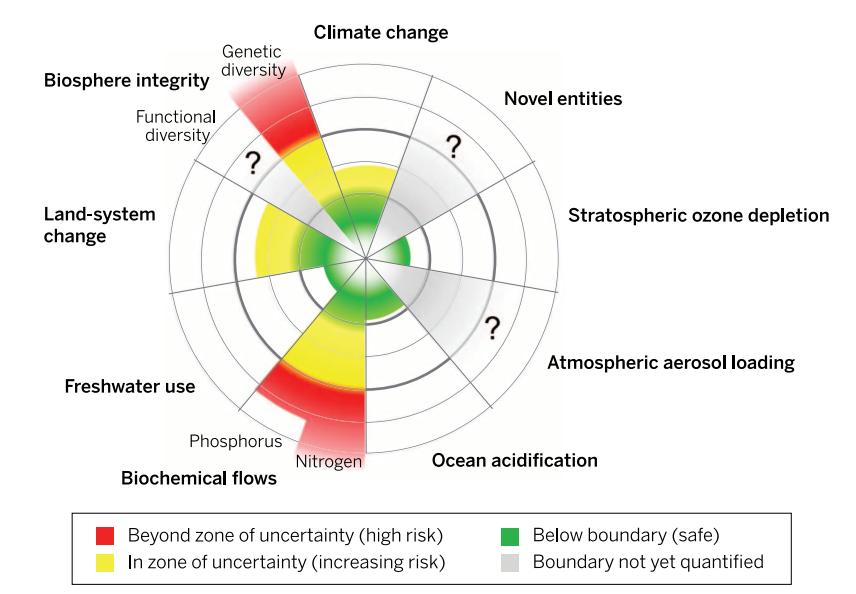
\includegraphics[width=1\linewidth]{./figures/planetary_boundaries} \caption[Planetary boundaries]{Visualisation of planetary boundaries, source: Steffen (2015).}\label{fig:unnamed-chunk-5}
\end{figure}

The Earth system model defines boundaries of that limited variability as ``a safe operating space for humanity.'' However, this model does not reckon with the complexities of social systems. To rectify that shortcoming, Kate Raworth (\protect\hyperlink{ref-raworth_safe_2012}{2012}) has proposed to integrate the planetary boundaries model with the indicators of social priorities under the UN Sustainable Development Goals, thus creating a model of ``safe and just operating space for humanity.''

\hypertarget{doughnut-between-the-social-foundation-and-the-environmental-ceiling}{%
\subsection{Doughnut: between the social foundation and the environmental ceiling}\label{doughnut-between-the-social-foundation-and-the-environmental-ceiling}}

Raworth has advanced her integrated model to highlight that while the effects of historical and present transgressions of planetary boundaries endangering ``safe space for humanity'' have to be brought back within the pre-industrial era limits, never has all of humanity lived inside the ``just space'' of the fulfilment of social needs --- and thus her framework provides a tool to benchmark different trajectories of social transformation that would enable all societies to reach that goal (\protect\hyperlink{ref-raworth_safe_2012}{Raworth 2012, 8}). Doing so, however, would require a departure from the present economic system toward a system that would equally:

\begin{itemize}
\tightlist
\item
  pursue the social, economic, and environmental goals of sustainable development;
\item
  re-orient economic activity away from growth for the sole purpose of growth;
\item
  and measure achievement in indicators other than GDP (\protect\hyperlink{ref-raworth_safe_2012}{Raworth 2012, 8}).
\end{itemize}

In designing her model, Raworth has used the planetary boundaries model not only as a point of departure but also as a representation from which to formalise her own model. Interpreting planetary boundaries as an environmental ceiling that should not be breached, she has inscribed inside that ceiling an inner circle of social foundation that societies should not fall short of. These two circles form a doughnut-shaped space representing the ``safe and just operating space.''

\begin{figure}
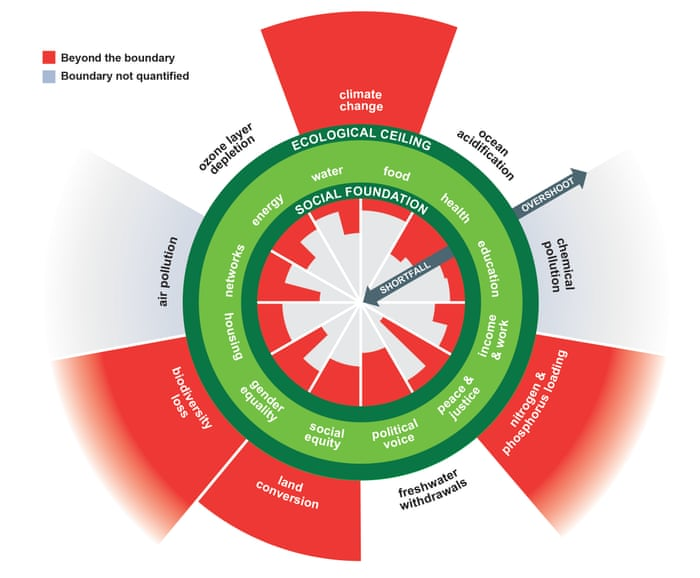
\includegraphics[width=1\linewidth]{./figures/raworth_doughnut} \caption[Raworth's doughnut model]{Raworth's doughnut model, source: Raworth (2017).}\label{fig:unnamed-chunk-6}
\end{figure}

Raworth's doughnut (or lifebelt) integrates environmental and social realities. It also acts as a policy tool to develop, steer, monitor, and compare future transition scenarios, filling the space between the description of the present reality and the aspirations of achieving social wellbeing within planetary boundaries. It sets two normative constraints on those scenarios: that everyone should be able to achieve the social foundation, while everyone should remain within their environmental ceiling. However, an environmental policy might have negative social impacts (e.g., regressive carbon tax), just as a social policy might have negative environmental impacts (e.g., fossil-fuel subsidy). There are only certain strategies within those constraints that do not come with such a trade-off (e.g., corporate carbon tax with an earmarked dividend or closing of a polluting factory with the opening of jobs in ecosystem restoration). The doughnut thus defines a narrow bandwidth of possible strategies of transition, but it still leaves space for different strategies that can be specific to different contexts. Also, it was developed with different scales of application in mind --- from global to national to regional to local. For instance, Raworth has been tasked by the City of Amsterdam to adapt the model to steer its sustainability transition so as to secure the wellbeing of its citizens, while remaining within its justly apportioned global share of planetary capacities.

Dan O'Neil and his team (\protect\hyperlink{ref-oneill_good_2018}{2018}) have assembled the dataset for Raworth's initial model for all countries, concluding that at present no country fits within the doughnut (\emph{Figure 6.3}). For good measure, the universal achievement of some of the more demanding goals of the social foundation, such as democracy, equality, or secondary education, would require, using current technological and institutional provisioning systems, ``resources 2-6 times the sustainable level'' (88). That is a daunting prospect if it is to be achieved for a global population. It would require a drastic restructuring of provisioning systems (infrastructures, technologies, manufacturing, governments, communities, markets\ldots) and a re-orientation of social needs toward sufficiency instead of maximisation of needs-satisfiers. It also indicates that the most affluent nations that do well on those goals of the social foundation, such as Nordic social democracies, do not offer a scalable model of development for the less affluent nations, requiring us to re-think what post-development in global terms might be.

\begin{figure}
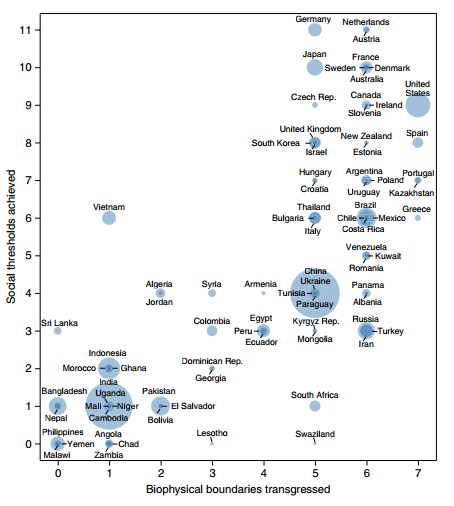
\includegraphics[width=1\linewidth]{./figures/oneill_countries} \caption[No country reaches the social foundation while remaining within the biophysical boundaries]{No country reaches the social foundation while remaining within the biophysical boundaries, source: D. W. O’Neill et al. (2018)}\label{fig:unnamed-chunk-7}
\end{figure}

\hypertarget{the-degrowth-doughnut}{%
\subsection{The Degrowth Doughnut}\label{the-degrowth-doughnut}}

The research team around IPE, led by Mladen Domazet, has acknowledged the conclusions of Dan O'Neill's team that the maximisation of needs satisfaction achieved by efficient provisioning might not bring us into a safe and just space for humanity, so we might need a conceptual model that starts from sufficiency rather than technological and economic efficiency and needs maximisation. Furthermore, Domazet and his team have, in their contribution to the \emph{Encyclopedia of the World's Biomes}, argued that Raworth's doughnut, by placing the overshoots of the environmental ceiling on the outer rim and the shortfalls against the social foundation on the inner rim, proposes a conceptual model that simply assumes a ``zero-sum trade-off'' (\protect\hyperlink{ref-domazet_mental_2020}{Domazet et al. 2020b, 7}) between society and nature, a binary opposition characteristic of the capitalist ecology that has dominated modernity hitherto and that has to be transcended if humanity is to transition toward a safe and just space for all. To reckon with these two shortcomings of Raworth's model, the researchers at IPE have developed their own doughnut.

Unlike Raworth's, the Degrowth Doughnut (\emph{Figure 6.4}) places biophysical and socioeconomic indicators, to which it adds a third set of cultural indicators, both at the outer and inner rim. The biophysical segment includes indices for climate change, biodiversity and agriculture, the socioeconomic segment for material security, health, energy \& materials, and democracy, and the cultural segment for wellbeing, environmentalism, and democratic potential. In contrast to Raworth's model, some biophysical indices, such as afforestation or organic soil, register shortfalls in human restorative action addressing measures which would be equally beneficial for society and nature. Conversely, some socioeconomic factors such as overwork or cultural factors such as anthropocentrism can have overshoots that result in negative impacts on both humans and the environment.

\begin{figure}
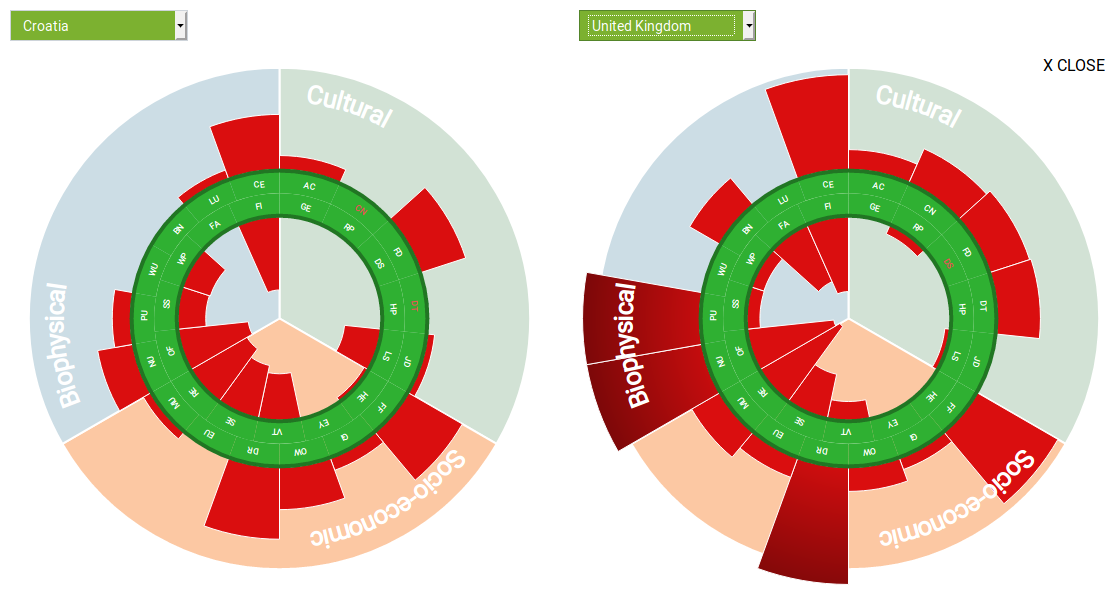
\includegraphics[width=1\linewidth]{./figures/degrowth_doughnut} \caption[Degrowth Doughnut: comparison between Croatia and the United Kingdom.]{Degrowth Doughnut: comparison between Croatia and the United Kingdom.}\label{fig:unnamed-chunk-8}
\end{figure}

The Degrowth Doughnut includes indices that were selected to reflect sufficiency rather than needs maximisation. For instance, instead of absolute life expectancy, the Degrowth Doughnut includes an indicator of healthy life expectancy that deducts years of poor health from the years of healthy life. Health rather than longevity is a better indicator of wellbeing, although the former can lead to the latter. Furthermore, among cultural indicators, it registers pro-environmental attitudes toward climate change, democracy, ecosystem restoration, and degrowth that are a prerequisite for an ecological transformation.

The outer rim defines the constraints between society and nature, whereas the inner rim highlights the restorative actions that lead to the mutual flourishing of society and nature. The inner rim includes thresholds as diverse as ``ecosystem restoration, sustainable food and energy provision, social equity, democratic participation, human health, wellbeing, and pro-environmental activation'' (\protect\hyperlink{ref-domazet_mental_2020}{Domazet et al. 2020b, 284}). Such a dialectical model, positing a connection between the necessity of limitation and the potentiality of restoration, defines ``the basics of 21st century just and sustainable life on which no society should be reneging'' (\protect\hyperlink{ref-domazet_mental_2020}{Domazet et al. 2020b, 284}).

However, it needs to be noted, the Degrowth Doughnut has certain limitations. Firstly, datasets for the indicators, particularly cultural, are lacking for many countries. One indicator, support for degrwoth, was developed by IPE and has data for only eighteen countries (\protect\hyperlink{ref-ancic_potential_2015}{Ančić and Domazet 2015}). This limits the ability to compare countries on that indicator. However, the missing indicators can be conveniently omitted from the doughnut to still allow for comparison between indicators that do exist. Or, they can be substituted with other indicators that reflect pro-environmental attitudes that are specific to a context to track the progress of a transformation over time that is specific for that context. Secondly, this begs the question as to why these indicators were selected. Raworth's indicators draw from two major research and policy efforts: the planetary boundaries model and the Sustainable Development Goals. But for this reason, they remain beholden to the assumptions of existing models, which do not factor in the change of sociometabolic system --- exactly the problem that is also reflected in Raworth's binary opposition between society and nature. Indicators in the Degrowth Doughnut are less grounded in the pre-existing analyses but have the benefit that they are more programmatic in their orientation toward degrowth and allow for plural future society-nature development trajectories while still retaining a universal framework of global constraints for those trajectories. Thirdly, an integrated assessment should satisfy a number of criteria (\protect\hyperlink{ref-pulselli_need_2016}{Pulselli, Moreno Pires, and Galli 2016}): it should be based on systems-thinking, be oriented toward the long-term transformation while offering guidance for localised action, consider equally production and consumption patterns, consider a fair distribution of burdens, address abosolute instead of relative indicators and causes instead of symptoms. While Degrowth Doughnut certainly does cover many of these aspects, it requires further research to establish if particular indicators are absolute and benchmark causes instead of symptoms. But as \protect\hyperlink{ref-domazet_mental_2020}{Domazet et al.} (\protect\hyperlink{ref-domazet_mental_2020}{2020b}) discuss, the Degrowth Doughnut is more akin to a scientific principle theory that offers ``a breakout from a conceptual impasse,'' and generalises abstract space of possible changes in the causal interactions, which ultimately points toward the transformation of the global social metabolism that all doughnut models aspire to.

While offering a conceptual model that integrates findings from environmental science and social sciences, doughnuts are primarily developed as a governance tool that might help develop, steer, monitor, and compare strategies to transition societies toward safe and just futures. Therefore, I would argue that they are a form of participation in the debates of the scientific ``extended peer community'' that advises policymakers, but also as \emph{an attempt to practically shift the frame of the debate and dominant institutional logic around climate action from reliance on the market to democracy at various scales of governance.} Doughnuts can visualise for everyone both the downscaled global environmental responsibilities and internal social responsibilities. They can be scaled down from countries to regions, and even smaller self-governing metabolic units, provided there is adequate data, and it is IPE's expressed intent to develop the existing online visualisation tool into a tool that could draw doughnuts for datasets at various scales.

\hypertarget{degrowth-as-a-new-political-imaginary}{%
\section{Degrowth as a new political imaginary}\label{degrowth-as-a-new-political-imaginary}}

With that experience of IPE's degrowth advocacy from the semiperiphery and against the background of the framework of the ``middle-ground'' strategic agency I devised in the previous chapter, in this last section I will discuss the transformations that the degrowth movement is proposing and the scales on which it is proposing them. Furthermore, I will argue through some of the criticisms of degrowth. And, finally, elaborate how its non-reductivist, multidimensional, and prefigurative strategy opens up to compositions of livable environmental futures --- in a ``full world'' that, as I will contend, has become rejective of most future-oriented strategies of social development.

\hypertarget{proposals-for-a-socially-sustainable-economic-degrowth}{%
\subsection{Proposals for a socially sustainable economic degrowth}\label{proposals-for-a-socially-sustainable-economic-degrowth}}

Degrowth's double objective of reducing ecosystems' overuse while achieving wellbeing is primarily addressed at affluent societies. It is the affluent societies that should lead the way in throttling down growth and redistributing social wealth domestically and internationally. By doing so they would relieve other societies from the competitive pressures of the capitalist growth-oriented system and allow them to pursue their own pathways to sustainable wellbeing, thereby securing a horizon of environmentally safe and just futures for all societies. Unless affluent societies lower the level of resource appropriation in a planned way, environmental degradation might reduce the economic base of many societies to a much smaller level (\protect\hyperlink{ref-stern_economics_2007}{Stern 2007}). In fact, climate instability has already widened the inequality between more affluent and less affluent societies by 25\% (\protect\hyperlink{ref-beuret_global_2019}{Beuret 2019a}). But also, in more affluent societies, a scaledown, if accompanied by a democratically deliberated redistribution of income, wealth, and power, might make sense for the many. For instance, after a certain level of affluence, it is not a higher level of income but a lower level of inequality that leads to higher life expectancy and better educational attainment (\protect\hyperlink{ref-wilkinson_greater_2011}{Wilkinson and Pickett 2011}). Welfare states with stronger public provision for social needs contribute to a greater sense of social wellbeing (\protect\hyperlink{ref-okulicz-kozaryn_subjective_2014}{Okulicz-Kozaryn, Holmes IV, and Avery 2014}). Lower disparities in income and power lead to greater environmental protection (\protect\hyperlink{ref-boyce_power_1999}{Boyce et al. 1999}; \protect\hyperlink{ref-raworth_doughnut_2017}{Raworth 2017}, ch.~3). As IPE researchers have found out in their study of 18 European countries, if a pro-environmental scaledown is implemented with a redistribution of wealth toward wellbeing and equality, a substantial part of the population might find it politically acceptable (\protect\hyperlink{ref-ancic_potential_2015}{Ančić and Domazet 2015}).

What follows from there, and as I have argued in chapter 5, is that \emph{environmental action has to be wedded to the problem of distributive justice and embedded into the everyday experience, addressing the apprehensions of popular masses over who is going to carry the cost of transition and instilling a practical grasp of the improvements to their social reality.} To instil that grasp of how a post-capitalist social metabolism can be evolved within a capitalist world, degrowth has devised a variety of proposals of ``non-reformist reforms'' (\protect\hyperlink{ref-gorz_strategy_1968}{Gorz 1968, 6ff}), including:

\textbf{1. Economy and economics:} The economy has to be made substantive by capping resource use based on the limits imposed by planetary boundaries, while allocating those resources for human needs democratically and equitably (\protect\hyperlink{ref-gerber_search_2018}{Gerber and Scheidel 2018}). The system of production should have collectively agreed purposes and be maximally localised. It should be centred on social and ecological reproduction, prioritising relational and ecological goods --- such as care-labour and ecosystem restoration, and placing sufficiency before efficiency and productivity.

Fractional reserve banking, the creation of money by private banks, and debt above what is needed for intergenerational redistribution should be abolished to limit the financial rents that drive the dynamics of growth. Concurrently, the state should take control over the issuing of ``public money'' (\protect\hyperlink{ref-mellor_future_2010}{Mellor 2010}) to finance a social economy: ``a basic income or a job guarantee or to subsidise cooperatives, care services, environmental conservation or renewable energy'' (\protect\hyperlink{ref-kallis_introduction_2014}{Kallis, Demaria, and D'Alisa 2014, 13}).

GDP should be replaced with indicators that measure social and ecological integrity, such as the Genuine Progress Indicator or Index of Sustainable Economic Welfare, or more ideally, with multidimensional indicators such as doughnuts.

Polluting segments of the economy, such as the fossil-fuel industry, need to be rapidly divested from or repurposed for the provision of clean energy.

\textbf{2. Employment:} Lowering of economic output can lead to unemployment. However, the replacement of energy-rich fossil fuels might require more human labour (\protect\hyperlink{ref-sorman_energetic_2013}{Sorman and Giampietro 2013}). The working week should be reduced, workplaces shared (\protect\hyperlink{ref-shor_work_2014}{Shor 2014}), and jobs guaranteed to anyone who seeks employment (\protect\hyperlink{ref-unti_job_2014}{Unti 2014}).

\textbf{3. Investment:} Investments should be redirected away from unnecessary and harmful activities such as military, fossil fuel, and polluting industries, and toward achieving environmental sustainability in agriculture, technology, the built environment, and infrastructure. Investments should also be redirected toward financing public services and a cooperative solidarity economy (\protect\hyperlink{ref-johanisova_co-operatives_2014}{Johanisova, Suriñach Padilla, and Parry 2014}).

\textbf{4. Income and taxation:} Societies should establish a universal basic income and universal access to goods such as food, housing, and care to meet the basic needs of all its members while also placing a cap on maximum income and taxing wealth to limit disparities. Taxes should shift from taxation of labour to taxation of resources and pollution.

\textbf{5. Technologies:} Green technologies should replace polluting technologies, however gains in efficiency and productivity should be translated into caps on resources and reduction in working hours to prevent a rebound effect or the expansion of extractive production (\protect\hyperlink{ref-alcott_impact_2010}{Alcott 2010}). Technologies should be developed under open license arrangements and should be manufactured locally, while research and development should be done through a global collaborative effort (\protect\hyperlink{ref-medak_technologies_2018}{Medak 2018}).

\textbf{6. Restoration of ecosystems:} Downscaling the global throughput of matter and energy will not be enough to ensure planetary ecological stability -- halting the sixth mass extinction and arresting the climate change. Degraded ecosystems need to be restored in order to effectively remediate the destructive effects already unleashed by the growth imperative. Expanding nature's protected areas, afforestation, agroecological farming, and the development of other mutually restorative practices between society and nature are the way to increase ecosystems' reproductive capacity.

\textbf{7. Democracy:} Degrowth assumes that social transformations cannot be implemented top-down but require a collective transformation of ways of living built on private sufficiency and public abundance. To achieve a transformation and evolve new patterns of production and provision will require a collective deliberation over those processes and a direct democratic power of members of sociometabolic units. This has led to a growing recognition of the importance of ``direct democracy'' (\protect\hyperlink{ref-kallis_degrowth_2018}{Kallis 2018}) and ``democracy in the workplace'' (\protect\hyperlink{ref-barca_labors_2017}{Barca 2017}) within the degrowth movement. While capitalism is premised on the institutional separation of the economic from the political (\protect\hyperlink{ref-meiksins_wood_separation_1981}{Meiksins Wood 1981}), a key condition for a degrowth transition is to re-embed economic processes within the realm of social needs and political deliberation. In more radical proposals, this calls for a devolution of power to smaller political units of social organisation such as local communities and municipalities, along the lines of communalism or ecological municipalism where democratic municipalities confederate (\protect\hyperlink{ref-bookchin_social_2007}{Bookchin 2007}).

\textbf{8. Decolonial pluriverse:} The degrowth movement maintains solidarities with the environmental justice movements and livelihood environmentalists of the Global South (\protect\hyperlink{ref-martinez-alier_socially_2009}{Martinez-Alier 2009}). Affluent societies should repay both colonial and environmental debt through reparations and reparation ecology (\protect\hyperlink{ref-moore_unearthing_2017}{Moore and Patel 2017}) while fostering global collaboration in shared technologies for localised systems of clean production and globally coordinated efforts of cleanup. They should acknowledge colonial and racist legacies by creating preconditions for non-competitive development. However, rather than imposing a unitary developmental model imported from the Global North, post-development allows for a pluriverse of cultures and economies (\protect\hyperlink{ref-kothari_pluriverse_2019}{Kothari et al. 2019}), where societies get more leeway from the global capitalist economy to create their own pathways to locally just and globally sustainable futures.

\hypertarget{scales-of-transformation}{%
\subsection{Scales of transformation}\label{scales-of-transformation}}

These proposals are not without contradictions. On the one hand, they aspire a global transformation, or at least a coordinated action between the Global North and the Global South. But to become politically feasible, the transformation has to start from national or preferably local metabolic units. However, this contradiction between the global condition and the local contexts as parallel grounds of action is inscribed in the ``middle ground'' where most of the degrowth actors are situated --- i.e., between the poles of largely (trans/sub)national governance that promulgates policies and of largely intra-social lived realities and distributive conflicts involving different social constituencies (see \emph{Figure 5.1}). What the discussion of IPE's work and the set of proposals listed above indicate, with important implications for my ``middle-ground'' strategic agency framework, is that \emph{the gap and struggle between the global governance and the local social realities is not mediated through and resolved only on the policy terrain, but equally on the institutional terrain of the economy, welfare provisions, and infrastructural arrangements --- at all of which degrowth targets its many proposals and innovations.}

However, as a strategy of global transformation, degrowth has been vehemently criticised by the scholar of global inequality Branko Milanović. Milanović claims that degrowth is magical thinking because it, supposedly, entails a convergence of income of global populations to the world median of US\$16/day (\protect\hyperlink{ref-milanovic_illusion_2017a}{Milanović 2017a}, \protect\hyperlink{ref-milanovic_illusion_2017}{2017b}, \protect\hyperlink{ref-milanovic_degrowth_2021}{2021}). In Milanović's' view, it is a politically unfeasible proposition as it would require 86\% of the population of the higher- and middle-income countries to renounce their higher incomes. It could be debated if this is a fair representation of degrowth positions, as degrowth envisions a plurality of socioeconomic pathways that do not fit the pattern of resource-intensive capitalist development --- if for no other reasons, at least for the reason that this developmental trajectory is for environmental reasons not available to the entire humanity. Nevertheless, \protect\hyperlink{ref-kuhnhenn_societal_2020}{Kuhnhenn et al.} (\protect\hyperlink{ref-kuhnhenn_societal_2020}{2020}) propose two comprehensive societal transformation scenarios focusing on transport, housing, food production, and technologies --- and not income --- that would lead to a convergence between the degrowing Annex I countries under the Kyoto Protocol (i.e., industrialised and industrialisng) and the growing non-Annex I countries to more easily achieve the decarbonisation goal of staying below 1.5°C.

Still, it remains a non-trivial task to orchestrate societal changes and socieconomic redistribution at a global level. But if we view this predicament from the perspective of the future degradation of planetary ecosystemic resources, there might be magical thinking in the assumption that the distributive conflicts over the access of economic resources can be avoided at the international level. The continuation of fossil-fuelled ``business-as-usual,'' but also an inadequate and untimely growth-oriented transition might, as scientists warn, result in significant costs, reduction of GDP, and displacement of people under climate stress. Assuming that the capacity of adaptation to climate change impacts such as heatwaves, floods, and droughts is also dependent on economic resources, the global poor will struggle to adapt. They might, however, contra Milanović's crown argument suggesting that migration is motivated by a desire for a better life and the ability to buy more stuff (\protect\hyperlink{ref-milanovic_illusion_2017}{Milanović 2017b}), be forced into migration not only because the grass is greener in the affluent North, but because no grass can grow in the climate-stressed regions of the South. The redistribution will thus necessarily happen in the form of climate migration if no other. The question is, therefore, whether the inter-societal redistribution of costs and capacities for climate action will unfold in a coordinated or a chaotic way, and whether the Global North can leave some of its carbon budget for the poorer nations, allowing them to pursue their own pathways and help them achieve sustainability through social, financial, and technological support. \emph{That question of inter-societal redistribution, as I analysed in the previous chapter, might become only politically feasible once the frame-shifting events, i.e., climate change-induced disasters, intensify.}

Another common critique of degrowth is that decarbonisation, ecosystem restoration, or economy of care all require investments and economic activities that will necessarily generate economic growth (\protect\hyperlink{ref-pollin_de-growth_2018}{Pollin 2018}). However, beyond the propositions of a steady state-economy that form one branch of the degrowth's pre-history (\protect\hyperlink{ref-daly_steady-state_1993}{Daly 1993}), degrowth has largely focused on criticising growth for the purposes of growth, growthism as an economic and ideological imperative, and the mechanisms of capitalist accumulation that are indifferent to the social and environmental purposes of economic activity. The purposes of economic activity --- an issue that Milanović's perspective of dollars and cents occludes --- should instead be sustainability, wellbeing, and justice, and not growth. A reason for concern from degrowth's perspective might be the ambitions of unprecedented scaleup of renewables and negative emissions technologies that will require a significant expansion of dirty extraction of clean metals risking an incursion on ecosystems and indigenous communities. However, the far greater and more immediate problem is that the continued extraction of fossil fuels contributes around 4\% of the global GDP and requires another 6.5\% of the global GDP in subsidies (\protect\hyperlink{ref-bailey_still_2021}{Bailey, Black, and Vernon 2021}). Rapid and deep degrowth in that segment of the global economy would result in enormous benefits, but to reap these benefits in a timely manner, some reductions in energy demand and accumulated financial wealth might be necessary (\protect\hyperlink{ref-semieniuk_stranded_2022}{Semieniuk et al. 2022}). \emph{Therefore, degrowth needs to specify its call to de-grow to specific sectors and forms of the economy, not only economic growth in general.}

Finally, the degrowth research community and its policy proposals can be criticised for having increasingly focused on the policy arena of mitigation rather than the practices of resilience and adaptation. However, this seeming bias is the consequence of dominant tendencies in climate governance. The potential failure of the technology-first approach and the growing distributive conflicts will make climate change politics messier but, as I have argued in the previous chapter, might open up space for proposing alternative pathways. Degrowth actors as political epistemic actors are justifiably engaged around framing struggles, as they might bring in significant long-term effects. Still, given the incumbency of economic interests and the weakened yet strong influence of the capitalist economy over transition, such alternative proposals might not get the governments to move their positions toward a more democratic-redistributive climate politics until it is too late. Eventually, I would argue with IPE's Vedran Horvat, \emph{that devising resilience and adaptation strategies might be just as significant to addressing distributive conflicts as the strategies of mitigation and the struggles over their costs.} With the strand of the degrowth movement that has been exploring ``nowtopias'' (\protect\hyperlink{ref-carlsson_nowtopia_2010}{Carlsson and Manning 2010}; \protect\hyperlink{ref-demaria_geographies_2019}{Demaria, Kallis, and Bakker 2019}), i.e., practices of communitarian sufficiency, vernacular resilience, and prefigurative social organisation (\protect\hyperlink{ref-boggs_marxism_1977a}{Boggs 1977}; \protect\hyperlink{ref-rowbotham_fragments_2013}{Rowbotham, Segal, and Wainwright 2013}), oriented toward developing and supporting mutually sustaining relations between society and nature, the degrowth movement all this time did work on combining the registers of mitigation with adaptation necessary for communities pushed over the ecological brink.

\hypertarget{a-utopian-horizon-of-rejective-future}{%
\subsection{A utopian horizon of rejective future}\label{a-utopian-horizon-of-rejective-future}}

Given that the domination of the capitalist state as social formation has foreclosed the horizon of systemic change (see section 3.4), there is an urgency to re-instil into the political life a future-oriented, utopian yet practicable possibility of systemic transformation that can give plausible hope to the many. The climate crisis need not lead into the ``crisis-paralysis circuit'' (\protect\hyperlink{ref-masco_crisis_2017}{Masco 2017, 66}). However, the future as a dimension of transformation can no longer be assumed to be what it was in the past. The future connoted as endless progress emerged with Modernity, characterised by capitalist dynamism, growth, and expansion (\protect\hyperlink{ref-rosa_social_2013}{Rosa 2013}). With the overcoming of the old pre-capitalist order built on stability and hierarchy, the future became a projective empty time-dimension that was open to different trajectories of social development. But beyond Europe, it also opened an empty space-dimension, a frontier of colonial, imperial, and neo-imperial conquest. From a decolonial perspective, that future never was a progress but a concomitant imposition of feudalism, slavery, and capitalism premised on the racialised division of labour that continuously thwarted the attempts at national liberations and social revolutions across the colonial world (\protect\hyperlink{ref-quijano_coloniality_2000}{Quijano 2000}). The sense of progress implied a growing colonisation and destruction of the natural environments and of indigenous communities, of what was legitimated as empty territory.

The concept of the future in the present is radically different. It is a rejective future of a world that is full with the growing detritus of capitalist pollution on the planetary scale. Ecosystems have been exhausted beyond their regenerative limits, some irreversibly so, making only some futures livable in that ``full world'' (\protect\hyperlink{ref-daly_economics_2005}{Daly 2005}). This rejective future is unwelcoming, threatening with uncertainties of tipping points that even scientists are at pains to predict (\protect\hyperlink{ref-lenton_climate_2019}{Lenton et al. 2019}), facing us with the risk of inhabitability of densely populated regions of the world. It is, therefore, ecologically discriminatory of different strategies of future-oriented action.

One unsustainable yet unrelenting future trajectory is the continued fossil-fuelled frontierism that persists in the drilling and fracking, expansion into the Arctic, slashing and burning of the Amazon, landgrab in Asia and Africa. The land prospecting that the US, Russia, China, Brazil, some EU and Gulf countries are currently pursuing across the world is placing economic pressure on low-income countries to allow continued extractivism. The other side of that land grab is the displacement of people, the erection of border walls, and the build-out of ``armed life-boat politics'' (\protect\hyperlink{ref-parenti_tropic_2012}{Parenti 2012}; \protect\hyperlink{ref-mitropoulos_lifeboat_2018}{Mitropoulos 2018}). Against this frontierist trajectory of ``business as usual'' stands the trajectory of a market-driven technology-first transition that risks being neither adequate nor timely to prevent global warming significantly beyond 1.5°C. That risk thus enjoins the future-oriented action to the difficult combination of urgency, precaution, and experimentation in discovering and devising alternative trajectories.

Degrowth's response to that difficult challenge is threefold. Firstly, a response of, in Isabelle Stengers words, learning to compose with ``the voices of many peoples, knowledges and earthly practices'' novel trajectories, ``the terrible difficulty of which it would be foolish and dangerous to underestimate but which it would be suicidal to think of as impossible'' (\protect\hyperlink{ref-stengers_catastrophic_2015}{Stengers 2015, 50}). Secondly, a response of transforming the existing institutions and social structures through ``real utopias,'' i.e., viable social innovations that instantiate under present conditions institutions of sustainability and justice (\protect\hyperlink{ref-wright_transforming_2013}{Wright 2013, 17}). Thirdly, a response of changing the terms of the debate around future-oriented action, from a reductivist action narrowed down to decarbonisation, to one of integrative sustainability, wellbeing, and justice.

Politically and ecologically, having available ever greater quantities of cheaper consumer goods whose globally organised production accrues wealth to the few is not what sustains societies. This is the dynamic of a system of capital accumulation and not the dynamic of a system of social needs. What sustains societies is a collective deliberation on how the necessary social labour of providing food, shelter, health, care, education, and a couple of other things can be organised so as to restore our planetary environments and leave us more free time from the necessary labour for our self-determinative individual and collective engagement with the world. The responsibility that this time is well spent is ultimately what defines our finite time (\protect\hyperlink{ref-hagglund_this_2019}{Hägglund 2019}) and a commitment to livable futures in this world we share. As I have shown throughout this chapter, degrowth largely offers a strategy that attends to that responsibility. The question is, however, will the unwelcoming and rejective future that interpellates us to experiment and act with urgency and precaution make its sobering, unpopular, and radical call to throttle down growth in destructive parts of the economy enough of a necessity before a large part of the living world risks being rejected from that future. After all, to serve as a cautionary tale, the last 35 years since James E. Hansen warned the US congress of anthropogenic climate change have largely been spent in inaction.

\hypertarget{working-class-environmentalism-environmental-agency-of-an-industrial-trade-union}{%
\chapter{Working-class environmentalism --- environmental agency of an industrial trade union}\label{working-class-environmentalism-environmental-agency-of-an-industrial-trade-union}}

\minitoc

\hypertarget{introduction-conflicting-environmentalisms}{%
\section{Introduction: conflicting environmentalisms}\label{introduction-conflicting-environmentalisms}}

In this chapter, I am continuing with my exploration of the ``middle-ground'' actors and their respective varieties of environmentalism. In the previous chapter, I have discussed degrowth as a movement and a disruptive reframing of environmental action that approaches the planetary environmental crisis with rigorous scientific realism. Degrowth is advocating that affluent societies throttle down their demand for energy and matter and redistribute social wealth domestically and internationally. This would open paths to social metabolisms whose environmental impacts are brought back within the limits of planetary boundaries and allow all societies to achieve environmentally safe and just futures in the destabilised ``full world'' (\protect\hyperlink{ref-daly_economics_2005}{Daly 2005}).

However, degrowth's proposition is frequently viewed, even by its proponents, as a political hard-sell: the transition it envisions would require a voluntary limitation of impactful processes and thus a radical transformation of patterns of production and provision that shape the everyday realities in affluent societies. Its critics on the left, notably the Marxist geographer Matthew Huber (\protect\hyperlink{ref-huber_ecological_2019}{2019}), fault degrowth's vision as negative and incapable of popular mobilisation --- because the working class in the affluent capitalist countries has over the last four decades been subjected to a depression of wages, unemployment, and austerity, leaving it in a growing need for more of the material wealth that their increasingly unequal societies have accumulated to the few.

While degrowth advocates have placed the redistribution of social wealth front and centre, according to Huber it is the concentration on the excesses of consumption and the virtues of subsistence economies --- in short, on middle-class ``lifestyle'' and minoritarian ``livelihood'' environmentalism --- that make it inadequate in addressing how the planetary ecological crisis impacts the lives of the majority of the global population whose subsistence is dependent on selling their labour in exchange for wages to buy commodities.\footnote{As discussed in section 5.6, the majority of the global population living in urban settlements depends to some degree on the commodity economy, as does a large segment of the global population living in the countryside.}

With this criticism in mind, in this chapter, I am shifting the focus to working-class environmentalism. Borrowing the notion, in fact, from the degrowth scholars Stefania Barca and Emmanuele Leonardi (\protect\hyperlink{ref-barca_working-class_2018}{2018}), I want to contend that \emph{the two sites of environmentalism --- social movements and the working class --- are in the present conjuncture in need of a unitary analysis of struggle against the tradition that regards them as separate forms of struggle located in distinct social spheres --- inside and outside of the sphere of capitalist production}. This chapter works toward that goal.

The environmental movement started to coalesce into its present form in the late 1960s and the 1970s as a critique of industrial society and its depredations on nature. It joined a tide of emerging social justice struggles against patriarchy, racism, and imperialism. Disenchanted with the waning militancy of organised labour, the failure of the industrial working class to build a larger opposition to capitalism, and the inability to transcend the gendered, racialised, and imperial forms of domination that persisted inside and outside of the factory, the new left shifted its interest from the tradition of working-class organising toward a movement of movements inclusive of a variety of struggles: feminist, anti-racist, anti-imperialist, indigenous, environmental, and, now on equal footing, labour. André Gorz, who coined the notion of degrowth, argued at the time that the desire for socialism oriented toward growth-based middle-class social patterns is ``the continuation of capitalism by other means'' and that the ecological struggles have to remain separate for as long as the radical left has not embraced ecological principles (\protect\hyperlink{ref-gorz_ecology_1980}{Gorz 1980, 13}). The conflicts over polluting industrial activities have frequently pitted environmentalists against the material interests of workers whose jobs depend on polluting industries.

And yet, while the environmental movement --- and increasingly the mainstream of environmental science --- see it as necessary to radically transform the existing capitalist societies, for Huber (\protect\hyperlink{ref-huber_ecological_2019}{2019}) both the movement and the scientists fail to grapple with the fact that system change ``requires a confrontation with some of the wealthiest and most powerful sectors of capital in world history'' and that this momentous task necessarily involves the working class. In fact, the last half a century of post-working-class environmentalism has seen ``a massive shift of power toward the capitalist class'' (28), while failing to do enough to prevent the accelerating planetary ecological destabilisation.

Contra Huber, one could contend that the problem is that working-class organisations were not capable of preventing that power shift either and that today the most militant elements of environmental organising are far removed from the workplace. They are, on the one hand, spearheaded by grassroots protest movements such as Extinction Rebellion and youth-led Fridays for Future; and, on the other, directed by campaigns aimed at the chokepoints of extractivist infrastructures such as Ende Gelände or NoDAPL, frequently led by indigenous land protectors. Furthermore, with the rout of the Labour Party in the 2019 UK parliamentary elections and the defeat of Bernie Sanders in the 2020 US presidential primaries, the working-class-oriented Green New Deal (GND) politics has suffered significant setbacks. This defeat has again ceded the terrain to the proponents of green capitalism that are pushing for flexible, least-cost technology-first approaches while insisting on safeguarding economic growth and largely disregarding the environmental impacts beyond greenhouse gas emissions. While trade unions have a venerable history of environmental agency, for reasons related to the crisis of trade unionism, which I will discuss in this chapter, they came to climate action relatively late. Now with the waning fortunes of the political forces backing GNDs, they will have to re-orient themselves and find new alliances with, amongst others, environmental movements if they do not want to cede the terrain to the market-driven technological restructuring that portends another weakening of the working class and trade unionism. Toward the conclusion of this chapter (section 7.5), I will grapple with the strategic outlook of working-class environmentalism in the wake of these events.

But before I arrive there, at the centre of this chapter will be my case study of Unite the Union (section 7.4). In the early autumn of 2019, I conducted interviews with the representatives of Unite, planning to undertake in the ensuing months an exchange and collaboration within its internal environmental working bodies and discussions. The onset of the COVID-19 pandemic has disrupted this plan. At the same time, the convergence of the Labour defeat, Brexit, and the pandemic in the span of a mere year has significantly complicated the discussion of any future-oriented action for a trade union whose membership is through the convergence of these three factors facing significant uncertainties in the near-term. For these conjunctural reasons, the empirical evidence I will include will have limited scope. Instead, in an acknowledgement of these interceding developments, this chapter will bracket my case study of Unite as a ``middle-ground'' organisation with, on the one hand, a discussion of the environmental vulnerability of the working class (section 7.2), the structural underpinnings of the disruptive power of working-class environmentalism (section 7.3), and a future-oriented speculative reflection on the opportunities it can seize on in the present conjuncture (section 7.5).

I have chosen to analyse Unite, as a large industrial trade union in an affluent country of the European capitalist centre, for three principal reasons:

Firstly, Unite represents workers in some of the most polluting, difficult to transform or phase-out sectors such as coal mining, car manufacture, air transport, or agriculture. While it strictly acknowledges the necessity of urgent climate action, its groundedness in constituencies vulnerable to the sustainability transition implies that it navigates some of the hardest contradictions between the urgency of action and the long-term security of those workers and their communities.

Secondly, strongly in favour of tighter mitigation targets and coordinated government investments into innovation and just transition, trade unions such as Unite are ambivalently positioned toward the dominant ecological modernisation framing of climate governance. Sometimes they even advocate for technological solutions to create lifelines for existing industries, but are strongly rejecting market-driven solutions that shift the power over the transition into the hands of corporations.

Thirdly, Unite is affiliated to the UK Labour Party, allowing it to significantly impact the political terrain and help shift the framing of climate action while exposing itself to the pressures of progressive grassroots party-member initiatives such as Momentum (\protect\hyperlink{ref-momentum_us_2021}{2021}) and Labour for a Green New Deal (\protect\hyperlink{ref-labour_for_a_gnd_who_2021}{2021}) that work to impact trade unions' pro-environmental orientation.

By drawing on the analysis of the disruptive power of the organised labour and my engagement with Unite, I will claim that, as ``middle-ground'' organisations, \emph{trade unions are responding to the market-driven technology-first policy approach with epistemic interventions that highlight the central distributive aspect of industrialised formal economies --- that of stability and quality of waged employment}. Thus they are demanding a transition that preserves jobs and provides socialised security there where those jobs need to be phased out. On the terrain of policymaking, particularly in the corporatist contexts dominated by the tripartite social partnership, such as the UK, trade unions have the strategic position they can use to shift the dominant market logic of how governments approach climate action, but that shift is largely not away from growth or even productivity-enhancing technologies. The GND conjuncture has built partly on that frame-shifting capacity, aiming to depose the dominant market-driven approach and open space for a negotiation over different pro-environmental strategies.

Furthermore, judging from Unite's work on organising professional training programmes, \emph{trade unions can empower workers through reskilling and the greening of their workplaces to not be destined to polluting jobs and potentially become agents of pro-environmental action themselves.} The restructuring of the workplace and working knowledge can potentially mobilise broad working-class constituencies into environmental action starting from their working lives. Finally, trade unions in many countries, including the UK, are limited in using the disruptive power of strike without a demonstrable dispute with the employer, making it difficult --- even when there is willingness, as in the case of Global Climate Strike in 2021 --- for them to act as a vector of disruption in mass organising. Thus they remain reliant on wildcat strikes and social movements for disruptions, expansion of the right to unionisation, and larger political mobilisations.

\hypertarget{understanding-working-class-environmentalism}{%
\section{Understanding working-class environmentalism}\label{understanding-working-class-environmentalism}}

In defining working-class environmentalism and the strategic environmental agency of organised labour, it is useful to first flesh out the relations of society and nature as structured through capitalism. To do so would imply starting from the system of production. Why production? --- Because, as I have argued, production is central to organising the metabolic exchange between a society and its environment, and thus it causally defines the patterns of social consumption as well. By combining human labour and technologies in certain ways, production processes structure the way capitalist societies appropriate nature's resources, transform them for human use, and disrupt their reproduction. However, not all of the planetary nature is included in capitalist processes. This requires us to specify that inside-outside boundary separating external from economically-integrated nature, the value of that external nature to capitalism, and how its destabilisation impacts capitalism. Given that the dynamic of capitalist accumulation is driven by cycles of expansion and crisis, the question is how the two types of crises --- the economic and the environmental --- are related and how they impact the lives of workers and their communities.

\hypertarget{nature-inside-and-outside-of-capitalism}{%
\subsection{Nature inside and outside of capitalism}\label{nature-inside-and-outside-of-capitalism}}

Following Foster and Clarke (\protect\hyperlink{ref-foster_robbery_2020}{2020}, ch.~1), capitalism can be considered a system that has an internal structure and external conditions of reproduction (see \emph{Figure 7.1}). The internal structure, or, in Marxian terms, its mode of production, is premised on the process of capital accumulation. The process starts with money being invested into labour and technologies in order to produce commodities. The value in this process is generated through the exploitation of workers, i.e., the use of their labour to produce commodities in excess of what is necessary to cover the cost of investment into labour and technologies. However, to generate a surplus, a capitalist enterprise has to sell more commodities than the workers, capitalists, and investors combined can buy from their past wages, profits, and interests. Thus, to prevent a crisis of aggregate demand and overproduction, the money to generate that surplus has to be borrowed from the future, and the process needs to continue growing in order to remain sustainable. This growth, however, can only be maintained through either the expansion or the intensification of the system: ever-greater geographies and ever-broader aspects of life have to be drawn into capitalist processes.

\begin{figure}
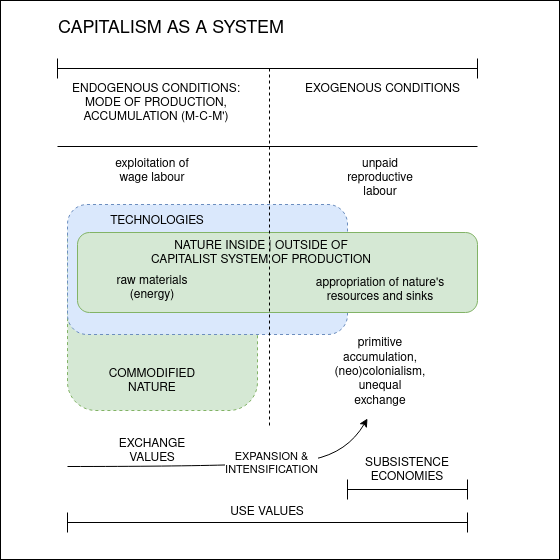
\includegraphics[width=1\linewidth]{./figures/nature_in_and_outside_capitalism} \caption[Nature inside and outside of capitalism]{Nature inside and outside capitalism and the processes of capitalist expansion and intensification into non-commodified social and natural domains.}\label{fig:unnamed-chunk-9}
\end{figure}

To keep expanding and intensifying, the system thus always needs an outside. There are at least three ways in which capitalism invades that non-capitalist outside:

\begin{itemize}
\tightlist
\item
  through the appropriation of the products of unwaged reproductive labour that takes care of biological, physical, and social reproduction of the workforce,
\item
  through the appropriation of sources and sinks that are not yet included in capitalist relations and are the free gifts of nature,
\item
  or the violent acts of enclosure and primitive accumulation, colonial plunder and slavery, or unequal exchange.
\end{itemize}

Thus, in opposition to the endogenous processes of the system's reproduction through economic accumulation stand the exogenous processes of its reproduction through accumulation by dispossession (\protect\hyperlink{ref-harvey_new_2003}{Harvey 2003}).

As \emph{Figure 7.1} indicates, nature is not only on the outside. The extraction of raw materials that are needed in the production of commodities is itself a commodified production process. Primary commodities that are extracted through mining, drilling, fracking, and farming provide raw materials for sophisticated industrial processes. Among them of particular significance are fossil fuels. The enormous expansion and intensification of capitalist growth since the beginning of the 19th century were made possible by fossil-fuelled technologies, leading to the development of one of the most profitable sectors of the capitalist economy --- fossil capital (see chapter 3).

The industrial transformation of raw materials, use of artificial fertilisers, forest clearing, and the burning of fossil fuels have produced pollution concentrated largely inside and around the place of production, leading to toxic workplaces and sooty towns. Yet after two centuries of growth, the indirect impacts have reached the planetary scale. Still, the effects that the production processes have on the inside and the outside of nature are different. The commodified inputs of nature that go into capitalist production are subject to economic rationality, and their use can be curbed by making --- be that through protest, labour organising, regulation, or pricing --- the pollution and harm to workers and communities expensive for companies. Conversely, the impacts on external nature accumulate over decades while the costs for societies are deferred a long time into the future. In particular, the depletion of natural sinks, such as the capacity of vegetation, soil, and oceans to absorb atmospheric carbon dioxide and warming, remains invisible for a long while. Capitalist production thus uses such free gifts of nature to externalise its detrimental effects. However, they cannot be externalised forever.

The significance of this dual position of nature --- inside and outside of the capitalist relations --- accounts for the historically dual sites of environmental organising: the workplace and the social movement. And while working-class environmentalism initially emerged localised around the workplace, today it is no longer so. As Huber (\protect\hyperlink{ref-huber_ecological_2019}{2019}) points out, the majority of the global population lives inside the capitalist commodity economy, and unlike the populations in the subsistence economies, they encounter nature --- food, energy, matter, and environment --- primarily mediated through the commodity-form. The processes inside the system of production are the structural drivers of anthropogenic ecological destabilisation. However, the effects of externalised disruption of nature, regardless of their delayed manifestation, necessarily return back to where they were produced. The problem, which Huber, speaking from the US, tends to underplay, is that it does so in a highly uneven fashion for the working-class communities across the globe, particularly as the polluting industries have become increasingly based outside of the Global North. Instead, as I will contend, \emph{for the effects of the planetary ecological crisis to register as affecting the working class, the working class composition has to be considered from a global uneven and combined perspective.}

\hypertarget{uneven-and-combined-vulnerability-of-the-working-class}{%
\subsection{Uneven and combined vulnerability of the working class}\label{uneven-and-combined-vulnerability-of-the-working-class}}

This chapter, with its focus on Unite and the GND, will be primarily discussing organised labour in the affluent countries of the capitalist core, but the majority of the global working-class is not living in those countries. Thus when discussing working-class environmentalism, we have to consider how a variegated and interdependent geography of ecological degradation affects the working class differently in a world where its sections are both connected and separated through a highly unequal yet combined global system of commodity production.

The first vector of the working-class vulnerability is resulting from the rise and the subsequent crisis of industrial development. The secular decline in the post-WWII capitalist growth generated by the dissemination of the industrial development model to Western Europe, Japan, South Korea, and then across the world, has by the 1970s led to the crisis of overproduction and profits in the Global North (\protect\hyperlink{ref-silver_forces_2003}{Silver 2003}, ch.~2; \protect\hyperlink{ref-brenner_economics_2006}{R. Brenner 2006}). This crisis was in the 1980s temporarily patched through a fiscal shakeup, followed by the massive relocation of manufacturing to China, the build-out of the logistical networks, and the ascendancy of information and communication technologies (\protect\hyperlink{ref-cowen_deadly_2014}{Cowen 2014}). These parallel processes resulted in the de-industrialisation and the abandonment of large swaths of formerly industrial landscapes, leaving in its wake toxic ruins and ruined communities across former industrial belts and infrastructural hinterlands (\protect\hyperlink{ref-brenner_operational_2016}{N. Brenner and Katsikis 2016}; \protect\hyperlink{ref-neel_hinterland_2018}{Neel 2018}). \emph{The de-development of industrial urban centres and extractive hinterlands has combined with a withdrawal of social safety nets and a growing inequality, reducing the capacity to bear the cost of and adapt to wildfires, droughts, and heatwaves resulting from climate change.} These processes, I contend, define the principal characteristics of the working-class vulnerability in what was once known as the ``First'' and the ``Second Worlds.''

The second vector of working-class vulnerability affects the parts of the world that Christian Parenti has pithily named the \emph{Tropic of Chaos} (\protect\hyperlink{ref-parenti_tropic_2012}{2012}). \emph{These are the sacrificial zones of the planetary mid-latitudes where the colonial conquest and post-colonial wars over the last centuries have crippled the countries from pursuing the pattern of Northern industrial development while at the same time undermining the resilience of native communities facing rapid changes to their habitats due to environmental destabilisation.} In those countries the stressors such as droughts, floods, land grab, and forest clearing are driving the internal migration, creating slums across growing megalopolises, pushing a small segment of that displaced surplus population to desperately attempt crossing deadly land and sea borders in the direction of affluent countries northwards in order to secure their own survival and the survival of their families. And yet, while the migration regimes of the Global North have changed over the last half a century, leading to the criminalisation of cross-border migration, their economies have welcomed this illegal migration to continue to exploit cheap labour, particularly in low-paying sectors such as farming. This border geography of criminalised yet encouraged illegal migration sustains the agricultural sectors in the south of the US and southern Europe, although it is also present in many other places where migrant populations offer a cheap reserve army of labour.

The third vector of vulnerability comes from the destabilisation of external nature. The last four decades have seen a two- to three-fold increase in zoonosis -- leaps of pathogens from animals to humans (\protect\hyperlink{ref-berger_man_2020}{Berger 2020}). Degraded ecosystems, with their complexity reduced to benefit the monocropping and industrial farming of animals, have a lowered inherent capacity to halt the spread of epidemics among the wild species (\protect\hyperlink{ref-wallace_dead_2020}{Wallace 2020}). Therefore ecosystem destabilisation is expected to spawn incidences of zoonosis at an increasing rate. The health of humans, livestock, and wildlife is connected through the stability of ecosystems. The historical processes of extraction of natural resources, reduction of complexity in habitats, and exploitation of labour in the present need to be viewed, as epidemiologist Rob Wallace (\protect\hyperlink{ref-wallace_dead_2020}{2020}) proposes, in terms of relational geographies of circuits of global capital where, for instance, pig farming in China is financed by the likes of Goldman Sachs and cattle farming in Amazon by the likes of Blackrock. The zoonotic leaps are intensifying in the interface zones in wild forests, but their structural drivers and social effects are primarily elsewhere.

In the pandemic, the working class across the globe has experienced a radical loss of security. Massive threat to health and life has been accompanied by massive furloughs. The lockdowns have revealed the fundamental dependence of societies on ``essential services.'' The frontline workers in health and elderly care, in cleaning and agriculture, or in transport, whose work is mostly invisible, devalued, and precarious, had no choice but to continue to go to work not to lose employment and income. As these low-paid ``sacrificial'' workers --- working-class people, overwhelmingly women, migrants, and people of colour --- could not afford to lose their income, their communities were impacted the hardest by the pandemic. The disease has largely remained on their side of the class, gender and race divide. At the same time, those who could shelter in place have experienced a rapid digitisation of most aspects of their everyday lives (\protect\hyperlink{ref-graziano_care_2020}{Graziano, Mars, and Medak 2020}). The pandemic has thus catalysed a situation where the planetary environmental degradation has returned back to the sender through the global variegated and interdependent geography: \emph{from the global centres of the capitalist system of production --- to the interface zones between the internal and external natures --- back to the highly unequal urban landscapes and abandoned migrant populations. A complex yet unitary crisis for the global working class.}

\hypertarget{two-environmentalisms-one-struggle}{%
\subsection{Two environmentalisms, one struggle?}\label{two-environmentalisms-one-struggle}}

Now, the question is how the terrain to act on that accelerating uneven and combined crisis is then structured from the perspective of the working class's strategic agency.

In the 1980s, the Marxist ecologist James O'Connor posited that the capitalist mode of production is characterised by two kinds of crises, two structural contradictions, and two paths that can lead out of those contradictions (\protect\hyperlink{ref-oconnor_capitalism_1988}{O'Connor 1988}). The first contradiction is the traditional Marxian contradiction between the forces and relations of production, resulting in cyclical crises of aggregate demand and overproduction, which can spill over into debt crises. These crises are resolved either through a restructuring of the forces of production --- by means of the international division of labour and labour-substituting technologies --- or through a restructuring of the relations of production --- with greater state interventions into the markets and more planning. In O'Connor's view, both restructuring tendencies lead to greater socialisation of production and pre-conditions for the transition to socialism. But these are just pre-conditions, not an immanent tendency --- more flexible capitalism is just as likely an option. And indeed, the neoliberal period has seen a restructuring of the forces of production that has led to greater global integration of production processes while resulting in social decomposition and worsening conditions for parts of the ever-larger global working class.

The second contradiction is between the capitalist system of production (wherein the first contradiction unfolds) and the general pre-conditions of this system in the form of human labour and external nature, which are produced and reproduced outside of the capitalist system of production yet appropriated by it. As capital expands, appropriating human labour and external nature without investing enough resources into reproducing them, it degrades them and creates crises of underproduction of its own pre-conditions. However, environmental and social degradation exerts risings costs on society, leading to the formation of social movements that struggle to force the capital to pay for those costs. \emph{The reproduction of these pre-conditions is regulated by the state and is hence ideologically and politically determined, fought over in a struggle between the ``political power of capital'' and the ``political power of social movements'' --- thus on the ``middle ground.''} While these concerns cut across class lines, ``problems of the natural and social environments are bigger problems from the standpoint of the poor, including the working poor, than for the salariat and the well-to-do. In other words, issues pertaining to production conditions are class issues, even though they are also more than class issues, which becomes immediately obvious when we ask who opposes popular struggles around conditions? The answer is, typically, capital\ldots{}'' (\protect\hyperlink{ref-oconnor_capitalism_1988}{O'Connor 1988, 37}).

From there, I would argue that while the perspective of the social movements might not be a class-based perspective, and in fact, there is a legacy of disagreements between the labour and social movements, effectively the working class faces both crisis tendencies --- in the factory and in the community. As they scale, they become a single crisis of the capitalist system and a single crisis for the working class, which is affected both \emph{as a result of the degradation of working conditions and the degradation of living conditions, creating a solid foundation for the two environmentalisms to intersect and act together}. O'Connor conjectures that over half of the total social product in the 1980s might be going into protecting and restoring pre-conditions of production and that capital shifts these unproductive expenditures to the credit system and fiscal sphere, deferring them into the future and passing them on to the state --- with redistributive risks for the working class, citizens and poorer nations.

\hypertarget{strategic-environmental-agency-of-the-working-class}{%
\section{Strategic environmental agency of the working class}\label{strategic-environmental-agency-of-the-working-class}}

In the previous sections, I have outlined how the capitalist system of production drives the planetary ecological crisis and the exposure of the working class to various dimensions of that crisis: in the workplace, in their community, in the international division of labour, and through the ecosystem destabilisation. In the second part of this chapter, I will explore the working class's strategic agency in the changing political terrain of environmental action. Firstly, I will situate in historical and structural terms the working class's capacity to collectively act and change the trajectory of social development. From there, I will narrow my focus specifically on the environmental agency of trade unions as organisations of the working class, teasing out the faultlines that shape their orientation in the environmental action arena. Finally, I will concretise and complicate such analytical framing by discussing the climate policy and environmental activities of Unite, the largest industrial trade union in the UK.

In the final part of this chapter, I will then proceed to reassess the strategic terrain for the working-class's environmental action in the present conjuncture marked by the political defeats of progressive green new deal forces and the potential failure of the technology-first strategies.

\hypertarget{working-class-collective-agency-and-social-change}{%
\subsection{Working class' collective agency and social change}\label{working-class-collective-agency-and-social-change}}

As I argued in chapter 4, the capacity of social actors to transform the structures of a society they live in is constrained and enabled by the interaction with other social forces through the institutional ensembles of the state and the capitalist economy. Their power is fundamentally relational, structured, and strategic. The relative power of various social actors is conditioned by the selectivities of those institutions and their own material and ideational resources they can draw on from other structures. These selectivities are predisposed toward actions that reproduce existing structures, but once their conditions of reproduction are in crisis, a larger strategic terrain opens up, allowing structural change. That relational agency in structure can be concretised through the working class's collective capacity to use the material and ideational resources it has attained in the workplace to disrupt and instigate larger social change.

The modern capitalist state, with its attendant political system, has co-evolved and is thus interdependent with the capitalist economic system. To achieve these integrational goals, the state wields coercive mechanisms of law and violence, as well as non-coercive mechanisms of ideology, civil rights, or welfare. These mechanisms have their own evolutionary trajectories, thus making certain aspects of the political terrain partly autonomous from the economic system. However, their relative autonomy implies that, inversely, significant aspects of the political terrain are directly entangled with the economic system. The most salient being those that define the relations of production: private property, limitations on intervention into the economy, and the labour market.

The strategic power of the working class emerges there where the political and the economic interact most tightly. The ascendancy of industrial capitalism, employing an army of labour attending to increasingly complex machinery, created a mass basis of workers who, by dint of their numbers and their skills, could pool together material resources and use their indispensability to the production process to organise, set demands, and, ultimately, withdraw their labour. \emph{The concentration and specialisation of industrial workers created prerequisites for the exercise of ``power from below''} that the political scientist Francis Fox Piven (\protect\hyperlink{ref-piven_can_2008}{2008}) has also analysed as interdependent or disruptive power. As discussed in chapter 3, the introduction of coal as a primary energy source created chokepoints along the extraction and transport lines that allowed miners and railway workers to disrupt key nodes in the expanding system of industrial production and thus set demands that led to gains in labour, social, and democratic rights in 19th century Britain (\protect\hyperlink{ref-mitchell_carbon_2011}{T. Mitchell 2011}). That disruptive power of industrial labour had structural effects on the development of capitalist societies at large.

The sociologist Adaner Usmani's cross-country analyses of the changing historical patterns of employment suggest the trajectory and scope of that power (\protect\hyperlink{ref-usmani_rise_2017}{Usmani 2017}). Comparing the employment structure data he has assembled for a number of countries dating back to the 19th century, Usmani has demonstrated that the relative size of the workforce employed in manufacturing, mining, construction, and transport, measured against the workforce employed in agricultural, services, commerce, and other occupations, is a structural indicator of the working class's disruptive capacity. When defined in those terms, the disruptive capacity is strongly correlated with both the levels of unionisation (\protect\hyperlink{ref-usmani_fortunes_2020}{Usmani 2020}) and the levels of democratisation and equality in societies (\protect\hyperlink{ref-usmani_democracy_2018}{Usmani 2018}). In fact, social and democratic gaps in late-developing economies turn out to be strongly correlated with the low levels of unionisation, while the low levels of unionisation turn out to be strongly correlated with the late start and early peaking of industrial development. Finally, the fall in unionisation turns out to be strongly correlated with the de-industrialisation in the high-income economies over the last fifty years. These findings indicate that capitalist development, with its large-scale and capacity-enhancing industries, has created pre-conditions for a growing disruptive power of the working class, enabling it to achieve democratic and social gains in the countries that have industrialised early.

\emph{Unlike the elite theories of power that see the strategic terrain of institutions dominated by the political and economic elites, the theories of non-elite power or power from below highlight the capacity of disruption --- the collective breaking of rules and the withdrawal from interdependent relations in complex institutional setups.} Here power is relational, strategic, and distributive, grounded in the combination of heterogeneous interests and interpretations in institutional ensembles of modern society. The central, material aspect in a distributive conflict is the capacity to threaten cost on the opposing side. To be able to level a significant ``disruption cost'' (\protect\hyperlink{ref-mcalevey_no_2016}{McAlevey 2016}) on a more powerful corporate or political actor --- that is, to be able to withdraw labour, risking wagelessness and unemployment, or cripple infrastructure --- requires mass organising that can pool together collective resources and communal solidarity to buffer those risks. That solidarity needs prior organising, consciousness-building, and community work. And that was the principal historical achievement of the working class organising into trade unions.

\hypertarget{trade-unionism-and-environmental-action}{%
\subsection{Trade unionism and environmental action}\label{trade-unionism-and-environmental-action}}

However, over the last half a century, in many high-income countries, union membership has fallen off the cliff. While the unionisation levels have always varied significantly between OECD countries, with the process of de-industrialisation and tertiarisation, large-scale industrial armies have been reduced in size and deskilled between the 1970s and 1990s (\protect\hyperlink{ref-troy_us_1990}{Troy 1990}). The restructuring was driven by the changing market forces and relations of production (\protect\hyperlink{ref-silver_forces_2003}{Silver 2003}). The rising costs of wages, social protections, and environmental regulations achieved by labour militancy, accompanied by a profit squeeze resulting from growing international competition, resulted in a backlash of anti-labour actions and policies promulgated by the governments of that period. Probably the most prominent has been the war waged on the National Union of Miners by the Thatcher government over the closure of collieries in 1984-1985, which eventually resulted in the obliteration of the 200.000 worker-strong UK mining sector. Arguably, the early exit from the then nationalised coal allowed the UK to become an early leader in decarbonisation. However, the defeat of organised labour led to the subsequent economic and social plight of entire regions of the UK that is felt to this day. As they were taught a lesson through that history, the potential of another restructuring of the fossil-fuelled industries as part of the current transition is justifiably perceived by trade unions as a matter of some risk --- both for the rights of the workers and for trade unions' own capacity to organise. Jobs in well-unionised and high-skilled sectors such as power generation, car manufacture, and aviation sectors are on the line, whereas green jobs concentrated primarily in the construction, agroforestry, conservation, and the emerging green tech sectors present a challenge to achieve the same level of quantity, quality, and unionisation.

The developments in the 1980s have put trade unions between a rock and a hard place. By the 1990s, the embattled situation narrowed the scope of trade-union activity to prioritise job, wage, and workplace protections. While the neoliberal retrenchment was rolling back the collective gains in labour and social rights, the trade unions' disruptive power seemed on the decline. The narrow focus of business unionism conflicted with the understanding that a renewal of trade unions' capacity to pull in an increasingly fragmented workforce and to struggle to maintain larger social protections for labour requires them to expand their work to communities and build out social movement unionism. That need for renewal, married with the growing climate change consensus, motivated the trade-union movement to become involved in the global environmental arena and to start creating alliances to prevent that climate action results in a detrimental impact on the working class (\protect\hyperlink{ref-snell_unions_2010}{Snell and Fairbrother 2010, 413}). However, as international trade-union structures started to integrate climate action into their strategies, e.g, the International Trade-Union Congress adopted in 2010 a resolution on ``combating climate change through sustainable development and just transition,'' \emph{trade unions remained caught in a dilemma whether to retard changes or to push for changes in a specific direction. In that conflicted situation, the strategic choices of individual trade unions aligned largely based on two factors: their strategic orientation toward social, market, or class actors and the expected distributive effects of environmental action.}

Richard Hyman proposed to view the historical orientations of trade unions along three tangents: social partnership with the state and the employers, bargaining oriented toward private employers, or class-based antagonism (\protect\hyperlink{ref-hyman_understanding_2001}{Hyman 2001}). While corporatist capitalist economies tend to favour the first and liberal capitalist economies the latter two, the strategies most trade unions pursue are varying degrees of all three. In response to climate change, trade unions have largely tended to follow a similar pattern of strategies. They were aligning more with the social-democratic politics that aims for continued growth with a socially managed technological restructuring, or more with the neoliberal politics that stresses multi-stakeholdership and norm-setting for equitable participation in the market-driven transition, or more with the class-oriented and socialist politics that is sometimes critical of the technologies and productivism and sees the radicality of crisis requiring a transformation of the relations and the purposes of production based on the socialisation of production and re-orientation towards social needs (\protect\hyperlink{ref-hampton_trade_2018}{Hampton 2018}; \protect\hyperlink{ref-felli_alternative_2014}{Felli 2014}).

To complicate the terrain, effective climate action seems to be largely defined by distributive conflicts and not by consensual collective action (\protect\hyperlink{ref-aklin_prisoners_2020}{Aklin and Mildenberger 2020}). Climate action commitments in some countries have proven to be effective regardless of the fact that other countries have reneged on international agreements. The temporary exit of the US from the Paris Agreement has not deterred other nations from pursuing strong commitments. The reason for this is that pro-climate action forces have prevailed over the interests of the anti-climate action forces. The implication is that certain economic sectors and workers in those sectors within those countries are bound to end up on the losing end of the climate action --- and that is determined on the political terrain. Environmental politics, therefore, sometimes cuts orthogonally to the left-right and capital-working class divides (\protect\hyperlink{ref-mildenberger_carbon_2020}{Mildenberger 2020}), hence progressive environmental policies require strong redistributional social policies (\protect\hyperlink{ref-bergquist_combining_2020}{Bergquist, Mildenberger, and Stokes 2020}). Trade unions with large constituencies bound to end up on the losing end of climate action, as the example of Unite will show, can embrace progressive environmental positions and actions primarily if such redistributional policies are in place.

\hypertarget{the-workplace-and-the-community}{%
\subsection{The workplace and the community}\label{the-workplace-and-the-community}}

The environmental action of trade unions frequently has to navigate those conflicting orientations and alignments. Still, as discussed earlier, working-class organisations can and have long acted on environmental issues both inside and outside of the workplace. In the 1960s, a number of large US industrial trade unions started to amplify concerns of their rank-and-file over occupational health and safety hazards in the mines and factories (\protect\hyperlink{ref-gordon_shell_1998}{Gordon 1998}). They played a notable role in the passing of water and air pollution legislation in the early 1970s. A groundbreaking industrial action over workplace pollution took place in 1973 against Shell, as the Oil, Chemical and Atomic Workers' Union (OCAW) led a strike and a boycott that was joined by a number of prominent environmentalist groups, including the Sierra Club, which entered the campaign aiming, amongst others, to foster trust with labour organisations. The campaign led the president of OCAW Al Grospiron to state: ``Organised Labor must emphatically support environmental cleanup efforts and must never get into the position of opposing such efforts on the grounds of economic hardship\ldots{} Our position must be that nearly all polluting facilities can be corrected without hardships to the workers and that in those few cases where corrections are not possible new job opportunities or compensation must be provided for the workers.'' (cited in: \protect\hyperlink{ref-gordon_shell_1998}{Gordon 1998, 460})

This was an early formulation of a \emph{just transition} principle. The OCAW took to operationalising that principle into a strategy in the 1990s by developing a proposal for a ``Superfund for the Workers,'' which would use a part of federal funds allocated to the environmental cleanup to finance the retraining of workers displaced by the environmental regulation. This was an effective instrument to advocate a strong green industrial policy aimed at shifting production to less toxic processes and products while providing occupational reskilling and social safety for the workers and their communities (\protect\hyperlink{ref-stevis_global_2015}{Stevis and Felli 2015, 2}). However, such policies, which also included universal healthcare and the founding of a socialist party (thus, in many respects precursors to the present new green new dealism of democratic socialists), promoted by the OCAW throughout the 1980s and 1990s, fell on deaf ears. This was already the period of a steep decline in its membership, eviscerating the strategic capacity of OCAW to carry out those plans. Just transition proposals were thus left by the wayside only to return in the second half of the 2000s, first internationalised through the work of Sustainlabour - International Labour Foundation for Sustainable Development founded in 2004 by Spanish trade unionists, and then diffused through the International Trade Union Congress and introduced in the UNFCCC Conference of Parties documents in 2010. This time, however, less as an effect of workplace militancy and more as a result of the combination of \emph{a strategy for trade-union renewal and a strategy to avert the detrimental effects of climate action on the working class}.

For as much as the unionisation and disruptive capacity seem to have waned from their heyday, trade unions still continue to be the largest non-religious membership-based civil society organisations. For instance, the UK Trades Union Congress has around 5.5 million members, whereas the International Trade Union Confederation has over 200 million members in 163 countries. That is a significant basis that could oppose climate action if conducted unfairly, but also a significant disruptive power to achieve decarbonisation on just and sustainable terms. To fully appreciate the potential reach of that disruptive power, I would suggest that it is important to consider the interdependence of the worker and the community, as well as the capacity of working-class organisations to mobilise beyond the workplace. The labour scholar and activist Jane McAlevey's influential \emph{whole worker model} suggests that a successful industrial action has to overcome the hurdle of organising the majority of workers in a workplace, but the disruptive power grows so much stronger if the workers organise with the support of their communities (\protect\hyperlink{ref-mcalevey_no_2016}{McAlevey 2016}). Thus, a key tactic in a labour dispute for workers is the ability to mobilise other members of their community, either individually or through organisations in the community --- religious, cultural, environmental. What matters to workers is not only wage and workplace conditions but the wellbeing of the community they live in. In turn, what matters to the community is the wellbeing of workers who are part of it.\footnote{This is evident in some of the largest labour disputes over the last decade in the US, some of which McAlevey has taken part in organising, which were successfully fought by teachers and nurses. They were able to mobilise parents and patients into their disputes by articulating them as struggles for better education and medical care in their communities. McAlevey, a former environmental organiser herself, is highly critical of liberal strategies aimed at achieving social change, which start from calling on external experts to do advocacy on behalf of workers or professional organisers to mobilise workers into a conflict to swing the opinion of the decision-makers, businesses, and media. A maximum power to achieve social change starts from organising the oppressed to be the agents of change.}

It is not surprising that the struggles McAlevey analyses have largely been organised in the public sector in professions dominated by the care labour of women. The growing fragmentation and precarity of the working class are resulting in a growing societal crisis of reproductive labour and care (\protect\hyperlink{ref-fraser_contradictions_2016}{Fraser 2016}; \protect\hyperlink{ref-huws_reinventing_2020}{Huws 2020}). This contradiction, \emph{amid high levels of commodity overproduction contrasted with high levels of societal and environmental underproduction --- O'Connor's double crisis --- can be resolved through a fundamental reallocation and revalorisation of labour.} This calls for a major shift in how production is organised and what it produces, following degrowth's proposals --- a shift from material to relational goods and a care economy, but also for weakening the centrality of competitive labour market in social integration. The reduction of working hours, more equitable distribution of care labour, and guaranteed basic services could be just some of the approaches.

\hypertarget{unite-the-union}{%
\section{Unite the Union}\label{unite-the-union}}

However, trade unions' environmentalism starts from the existing labour relations, technological base, and social metabolism. To understand both how their positions and actions reflect the distributive conflicts and the political, economic, and technological realities of that terrain, I will profile the strategies of Unite, a large industrial trade union in a country of the capitalist centre, with a significant part of its rank-and-file employed across polluting industries. This profile is based on an analysis of primary documents published by Unite, interviews conducted with its Director of Education Jim Mowatt and its Research Officer Colin Potter, and secondary publications.

\hypertarget{introducing-unite}{%
\subsection{Introducing Unite}\label{introducing-unite}}

Unite is the UK's largest industrial trade union, comparable in size to the UK's largest public-sector trade union Unison. It currently represents around 1.4 million workers from over twenty sectors, including aerospace, shipbuilding, and car manufacturing, chemical, cement, and steel industries, civil air transport, freight and logistics sectors, energy and utilities, engineering and construction, as well as agriculture. However, it is not exclusively oriented toward private industrial sectors, as its membership also counts workers in health, postal, and local government sectors. Unite was formed in 2008 through the merger of the Transport and General Workers Union and the Amicus union, and was subsequently joined by a number of other unions, including the Union of Construction, Allied Trades and Technicians. According to Unite's head of education, Jim Mowatt, the unions that merged into Unite had in the early 1980s a combined membership of 6.8 million. In my interview with Mowatt, as the primary reason for the membership decline he cites the changes in employment patterns due to the offshoring of manufacturing, technological change, and the replacement of old, unionised sectors with new, non-unionised sectors. Fragmented and smaller workplaces made it harder to unionise. Nonetheless, over the last couple of years, Unite has been successful in slowly growing its membership by around 200.000 (\protect\hyperlink{ref-unite_the_union_community_}{Unite the Union n.d.a}).

Unite self-defines as an open, diverse, and democratic trade union, focusing on workplace bargaining, industrial action, and public campaigning while being a progressive force for a fairer society (\protect\hyperlink{ref-unite_the_union_vision_}{Unite the Union n.d.b}). The three complementary aspects of Unite's work are international alliances, education, and political representation. On the international front, Unite is pursuing trade-union alliances, advocacy work, and campaigns to advance international solidarity, joint collective bargaining with common employers, and struggles against cuts in pensions, social services, and labour rights. To this end, with its US counterpart United Steelworkers, it has formed a global trade union Workers Uniting (\protect\hyperlink{ref-unite_the_union_workers_}{Unite the Union n.d.c}). On the educational front, it maintains two training centres, organising annually around 12.000 accredited courses both for union representatives and occupational training. Importantly, this includes environmental representatives and occupational training for climate jobs. As tends to be the case with large, established, and hierarchical membership organisations, many aspects of its self-definition are contested: for instance, the never-ending tenure of the recently retired General Secretary Len McCluskey or the political affiliation to the UK Labour Party (\protect\hyperlink{ref-mcnally_big_2021}{McNally 2021}; \protect\hyperlink{ref-sparrow_unite_2021}{Sparrow 2021}). On the other hand, such large organisations frequently contain a plurality of parallel structures that are built to complement the central mission of the organisation. In Unite's case, those can be evidenced in community organising such as through the Grenfell community organisation, which was formed before the tragic fire and was there ready to provide support to the survivors.

However, the affiliation to the UK Labour Party merits particular attention. The affiliation of trade unions to a single party is a peculiarity of the British political system. While these forms of affiliations do exist elsewhere, for instance between the French CGT and the French Communist Party, they are rare in industrialised economies, where trade unions tend to maintain distance from political parties, as they do not want to wed their interests to a political party's fortunes regardless of ideological affiliations. The affiliation of labour unions to the UK Labour Party, however, emerged historically, as the party ``was formed out of the trade union movement to give working people their own political voice. The link from the workplace to the party through the affiliated trade unions is what makes it unique to this day'' (\protect\hyperlink{ref-labour_party_affiliated_}{Labour Party n.d.}). Unite maintains a separate Political Fund for political campaigning and assisting MPs, MEPs, and councillors to get elected. During McCluskey's tenure, it had a strong say in Labour's internal politics and policies. This nexus, as my interviewees attest, has enabled trade unions to secure historical gains on employment rights, safety, and welfare while continuously giving them a seat at the political table for the benefit of the working class. This has had significant implications also on the environmental front, as the radical green new deal and green industrial revolution policies that promised to take the UK to net-zero by 2030 were hammered out and pushed through into the 2019 Labour Manifesto owing to the joined effort of the grassroots organisers acting through Momentum, Labour for a Green New Deal, and progressive trade unions, including Unite. However, Unite's arguably biggest success in political lobbying was pushing the third runway at Heathrow through the parliament --- an environmentally dubious decision (\protect\hyperlink{ref-mcnally_big_2021}{McNally 2021}).

\hypertarget{unites-environmentalism}{%
\subsection{Unite's environmentalism}\label{unites-environmentalism}}

Well before the 2019 Labour Manifesto, Unite has been actively articulating its own science-based climate policy and has been working with the UK Labour Party, public bodies such as Climate Change Committee, and industry bodies, advocating its own national-, sector-, and workplace-level proposals (cf. \protect\hyperlink{ref-unite_the_union_hope_2015}{Unite the Union 2015}, \protect\hyperlink{ref-unite_the_union_response_2019}{2019a}). With a diverse constituency, Unite can draw on technical expertise and factory-level experience from various industries. Furthermore, it is collaborating with a number of academic institutions, including King's College in London and Edinburgh University, to research particular issues such as agricultural policy or workplace environmental safety. Unite's current position is encapsulated in its policy paper \emph{Tackling Climate Change Crisis} (\protect\hyperlink{ref-unite_the_union_tackling_2019}{Unite the Union 2019b}). The principal concern of Unite's position is that if global warming has to be limited to 1.5°C, the required pace of decarbonisation cannot be achieved using flexible, least-cost market mechanisms, while the blind imposition of such mechanisms will necessarily have detrimental effects on workers and their communities.

The strategy to tackle climate change in Unite's view has three major planks: ``a balanced energy policy, a just transition to a low carbon economy, and the growth of climate jobs'' (\protect\hyperlink{ref-unite_the_union_tackling_2019}{Unite the Union 2019b, 5}). Let us quickly go through them as they are articulated in that position paper.

\textbf{A balanced energy policy:} A rapid phaseout of coal provided a low-hanging fruit for the initial decarbonisation of the UK's energy sector. It also left the workers and communities stranded, with no just transition plan by the government to help them out. The next phase of decarbonisation should not repeat that pattern. For the next phase, Unite envisions investments into new and old renewables, the build-out of a new generation of nuclear energy with small modular reactors, and, as a stop-gap, the retrofitting of the existing gas energy capacities with carbon capture, utilisation, and storage infrastructure to reduce their emissions. Unite is proposing that the government builds a national pipeline network to transport captured emissions and store them underground in abandoned oil wells, reducing the impact and extending the life of carbon-intensive manufacturing and energy generation (\protect\hyperlink{ref-unite_the_union_response_2019}{Unite the Union 2019a}). Mining is, as Colin Potter writes in his response to my interview questions, a ``necessary evil,'' given that recycling does not provide enough materials (per \protect\hyperlink{ref-hickel_less_2021}{Hickel 2021}, the world's recycling rate was at 9.1\% in 2018), while coal continues to be necessary to produce coke as feedstock in steel, glass, and chemical industries. To phase out coal feedstock in blast furnaces, it is necessary to first develop hydrogen as a secondary energy source. Hydrogen can currently be either produced through the expensive water electrolysis process powered by renewables (``green hydrogen'') or through the cheaper burning and carbon capture from fossil fuels (``blue hydrogen''). Adding up to 20\% hydrogen to natural gas could reduce by an equal amount the CO2 emissions in domestic heating. Unite's balanced energy policy is, thus, characterised by a gradual change of technologies, including the introduction of negative emissions technologies that make coal and gas cleaner and allow them to stay longer in use, giving more time to transition the workers in the coal mining and polluting parts of the energy sector to new, cleaner industries.

\textbf{Innovation and just transition:} Government needs to impose tight targets and steer the innovation in hard-to-decarbonise sectors (\protect\hyperlink{ref-unite_the_union_response_2019}{Unite the Union 2019a}). Aviation is projected to be the most difficult mode of transport to decarbonise, and it is reckoned that it will not be carbon-neutral before 2050 or even later. In Unite's view, aviation is essential for the UK, given its insular territorial position and the need to connect with world economies. Thus, Unite has joined the aerospace and air carriers consortium Sustainable Aviation that seeks to reduce emissions from air travel by means of designing more energy-efficient fleet and airport operations, producing alternative fuels from domestic waste and promulgating an industry-wide emissions offsetting scheme. However, these advancements require public investment in R\&D. As do other industries that might be hurt by rapid decarbonisation, such as car manufacturing which is struggling to meet the goals of the internal combustion engine phaseout, or carbon-intensive metals, glass, ceramics, and paper industries. These industries need government support in R\&D and reskilling to retain their internationally competitive position. In highly polluting industries that are facing phaseout, the government needs to secure retraining or new jobs there where the workers are based, protecting wage levels, labour conditions, and community welfare.

\textbf{Climate jobs:} Lastly, decarbonisation will create new jobs in construction, plant decommissioning, engineering, energy, and transport. That transformation would benefit from the on-shoring of production of steel and wind turbines, efficiency improvements to homes and factories, adding new jobs. As per the One Million Climate Jobs campaign, supported by Unite, by 2035 these measures would create an additional one million jobs while reducing emissions by 86\% (\protect\hyperlink{ref-neale_one_2014}{Neale 2014}; \protect\hyperlink{ref-jeffrey_climate_2021}{Jeffrey 2021}). An important element in that strategy is the nationalisation of public transport, water, and energy sectors.

Beyond the policy and campaign work around climate change in the UK, Unite is also active on the international front, pushing for a managed energy transition as a part of the Trade Unions for Energy Democracy, an initiative advocating democratic management and public ownership of energy infrastructures. However, unlike TUED, Unite in its documents does not make a mention of distributed, community-led generation of energy that could be enabled through a nationalisation, localisation, or commoning of energy production, nor does it discuss the modernisation of the power grid necessary for such a transformation. Its strategy pivots around large-scale, commercial, and centralised energy production.

\hypertarget{situating-unites-environmentalism}{%
\subsection{Situating Unite's environmentalism}\label{situating-unites-environmentalism}}

Viewed from the perspective of the Hymanian triangle of trade-union orientations toward the market, society, or class, \emph{Unite is articulating its climate policies overtly in social-partnership, anti-neoliberal, state-led yet frequently technology-oriented terms}: ``The UK must look beyond narrow `market-based solutions' like carbon trading schemes or a simplistic target-driven approach and commit to working on a tripartite basis with trade unions and industry to devise a more effective strategy'' (\protect\hyperlink{ref-unite_the_union_tackling_2019}{Unite the Union 2019b, 10}). The focus is on public investments into technological change and upskilling, a managed transition of workers from phased-out to new industries, and the re-nationalisation of large infrastructures. On the positions where Unite diverges from other progressive trade-union and environmentalist initiatives, such as advocating a balanced energy mix that includes nuclear energy, continued use of fossil fuels with carbon capture technologies, or on the continuation of open-pit mining and the extension of Heathrow, it does so, as both of my interviewees indicate, not only to protect the jobs of its constituencies but also for reasons that the social, economic, and technological realities of quick transition would inadvertently produce perverse environmental effects: limiting Heathrow expansion would move air traffic to other runways in the UK, increase taxiing time, and increase in-country flying, whereas phasing out coal mining would lead to less environmentally controlled imports to sustain feedstock needs. In Unite's view, investment in technologies such as carbon capture or the development of alternative fuels can significantly reduce the negative effects and extend the lifetime of polluting industries under terms that, for a period of time, can contribute to the Paris Agreement commitments.

As I pointed out in chapter 3, negative emissions technologies play a significant role in the national decarbonisation scenarios pledged under the Paris Agreement, allowing an overshoot in carbon emissions that can be later compensated for by these measures that are, for the time being, far from the maturity, investment, and scale required to fulfil that promise. And while Unite does not advocate direct air capture but rather capture in the controlled industrial processes, there is a lack of technological development, high deployment cost, and risks of leakage involved in capturing, transporting, and storing emissions (\protect\hyperlink{ref-anderson_trouble_2016}{K. Anderson and Peters 2016}; \protect\hyperlink{ref-moch_carbon_2022}{Moch, Xue, and Holdren 2022}). Similarly with aviation, as recently analysed by the political economists Gareth Dale and Josh Moos, strategies advocated by Sustainable Aviation are highly speculative and face significant biophysical and technological limitations (\protect\hyperlink{ref-dale_jet_2021}{Dale and Moos 2021}). Thus these solutions risk perverse environmental effects as well. Changes in corporate and collective behaviour such as greater recycling or caps on business travel, subsidising of land and sea travel, and longer holidays to account for slower travel might prove quicker in meeting the goals of rapid decarbonisation. However, \emph{policies aimed at reducing demand, barring major climate-induced social disruptions, present an even greater challenge for policymakers to embrace than the targeted and just transition policies, although I would see them both as necessary given the urgency to prevent runaway climate change and biodiversity loss.}

Furthermore, investments in retrofitting the existing carbon-intensive industrial processes and infrastructures to reduce emissions might prove economically and environmentally too costly as they retard the transition to cleaner technologies that are getting cheaper. Retrofitting might end up being a sunk cost without the competitive advantage that new technologies bring. However, the dropping price of wind and solar might not be a boon for the working class unless the state coordinates a just transition and maximises the benefits for the workers from the transition. Unite had witnessed that first hand when the Danish wind turbine manufacturer Vestas closed its UK plants in 2009, at the very moment when the government was announcing its plans for a large-scale renewable build-out. In spite of a wildcat occupation at the Isle of Wight plant and joint protests of trade unions and environmental groups, Vestas laid off 465 workers citing planning regulations and NIMBY-ism that made manufacturing in the UK unsustainable. However, according to the trade-union scholar Paul Hampton (\protect\hyperlink{ref-hampton_trade_2018}{2018}), facing an ``extremely anti-union'' company, Unite grappled to adequately support workers' occupation, and for this was criticised by the activists as ``business unionists and social partnership bureaucrats'' (166). Therefore the workers of Vestas joined the more militant Rail, Maritime and Transport Workers union. As is characteristic of transport trade unions, including the International Transport Workers Union, RMT was a more radical, class-oriented, and socialist trade union (\protect\hyperlink{ref-felli_alternative_2014}{Felli 2014}).

There is no doubt that Unite's orientation is strongly corporatist --- particularly as it holds strong leverage over political actors. The Labour affiliation and calls for nationalisation give that corporatism a democratic socialist outlook, but, to state the obvious, in the Conservative-dominated period, that has its limits. Even so, the Vestas occupation unfolded during the New Labour tenure, and the calls for nationalisation were dismissed. In that situation, the wildcat militancy, with its temporality of confrontation, could have politicised the matter. But the short-lived militancy has to alternate with a strategy how to create arrangements that can sustain jobs at risk or provide alternatives to workers over the long run, which Unite is keen on developing. Therefore, no one orientation can do both on its own.

There are elements of social movement unionism in Unite's environmental work as well. For instance, Unite is building on the long-standing activities around health and safety, initiated in the late 1980s within the Trade Union Congress, to extend union representation in the workplace to environmental issues. These activities expanded the health and safety representation in the late 2000s, under the heading of \emph{Green Workplaces} (\protect\hyperlink{ref-tuc_greening_2010}{TUC 2010}; \protect\hyperlink{ref-hampton_trade_2018}{Hampton 2018}), to activities aimed at combating climate change by reducing the environmental impact of the workplace, generating ``an unusually high level of engagement from both members and potential members'' (\protect\hyperlink{ref-tuc_green_2008}{TUC 2008, 8}). Unite is not only pushing for such environmental representation but has, in fact, included environmental representation and just transition into all its training courses, empowering workers to act as subjects of ecological transformation.

If analysed from the framework of a ``middle-ground'' agency that I have developed in chapter 5, Unite can be viewed in three distinct ways. Its political affiliation with Labour, its active participation in national policy consultation processes, and the stances it takes on climate action and just transition in public, position it as an epistemic actor within framing struggles. Unite can use its institutional leverage and its mass constituency to push the government and policymakers to move away from the dominant market logic toward a redistributive-democratic logic and to regard distributive concerns over job security and transitioning of workers to new climate jobs as central to sociotechnical change. Secondly, through its active participation in industry bodies such as Sustainable Aviation and the advocacy of innovations in carbon-intensive industries, it is partnering with industries vulnerable to decarbonisation policies seeking to help them transition, thus actively impacting the direction of sociotechnical transition. Thirdly, through its professional training programmes, it empowers workers through reskilling and the greening of their workplaces to not be destined to polluting jobs and, at the same time, to become agents of transformation in their workplaces and communities.

To Unite's great merit, rather than resisting decarbonisation, it has embraced its objectives even for its constituencies in industries that risk being phased out or reduced in the process. It even backed and then worked to persuade other unions to stand behind the radical 2030 net-zero goal of the 2019 Labour Manifesto (\protect\hyperlink{ref-waugh_labour_2019}{Waugh 2019}). \emph{As an epistemic actor, however, it is forced to articulate and balance out often conflicting realities of job security against adequate and timely climate action.} Given that the just transition agenda is not receiving an outright acceptance within the governance arena, Unite has to bank on lifeline innovations and longer transition periods for polluting industries, even though this might work out against the interest of these industries and their workers as renewable and green technologies become cheaper and gain a competitive edge. Particularly, after the loss of the 2019 elections, the odds are stacked against the transition strategies focusing on equity and justice, weakening further the position of trade unions and workers in polluting industries. But, instead of withdrawing from politics and focusing primarily on workplace trade-unionism, as seems to be the predilection of Unite's new General Secretary Sharon Graham (\protect\hyperlink{ref-graham_sharons_2021}{2021}), \emph{trade unions might in the post-GND moment need a renewed transformative vision, a re-orientation toward climate-vulnerable working-class communities, and a re-alignment with social movements to shift the terrain of environmental politics again to benefit its constituencies}.

\hypertarget{a-challenging-future-ahead-of-working-class-environmentalism}{%
\section{A challenging future ahead of working-class environmentalism}\label{a-challenging-future-ahead-of-working-class-environmentalism}}

In this chapter, I have argued that the two environmentalisms --- working-class environmentalism and social-movement environmentalism --- are structured around the dual position of nature in capitalism. Resources that are extracted, processed, and integrated through human labour and technology into the system of commodified production constitute the nature internal to capitalism. Conversely, ecosystems serve as a sink into which that system can offload its heat, waste, and pollution; it is an external nature that the system can appropriate as a free gift in the process of expansion and intensification. Both of these aspects make this external nature a condition of possibility for capital accumulation. The growing degradation of external nature has destabilising effects on communities and entire societies. Given that the reproduction of external nature historically has not been a direct cost to the process of production, these destabilising effects had and still have to be addressed on the political terrain of the state --- where the working class, social movements, and scientists struggle with capital and policymakers over the internalisation of social and environmental costs of that degradation. Therefore, from the thriving global cities to the de-industrialised hinterlands of the Global North, from the sacrificial environmental stress zones in the ``Tropic of Chaos'' to the migrant landscapes of slums in metropolises of the Global South and routes that lead northwards, environmental conflicts are inter- and intra-societal distributive conflicts over who gets to thrive and who gets to bear the cost of environmental destabilisation.

The working class's strategic capacity to contest social domination and ecological degradation on that terrain roots in its collective disruptive power that emerged in the context of mass industrialisation and has historically allowed the working class to make significant gains in labour, social, and democratic rights beyond the narrow remit of the workplace. Accordingly, the growing environmental degradation in the industrial economies in the 1960s and 1970s transformed working-class organisations into environmental actors concerned with a range of vulnerabilities from occupational health hazards to pollution affecting their communities. However, the ensuing period of neoliberal restructuring saw manufacturing relocate to countries with fewer environmental protections and a less organised labour, while the automation, tertiarisation, and emergence of new, non-unionised sectors, decimated trade union membership, forcing unions to drop the environmental concerns over more pressing issues --- only to return to them as the debates around climate change and just transition gained momentum in the aftermath of the 2008 global financial crisis.

That watershed moment of 2008, marked by a convergence of jobless recovery and the growing evidence of climate change, birthed in the US and across Europe a configuration of progressive social forces and progressive environmental proposals that coalesced around the idea of a green new deal. Around the same time, in the wake of the Copenhagen COP15 meeting's failure to achieve binding commitments to emissions reductions, groups of indigenous peoples, campesinos, and climate justice activists from around the world descended on Cochabamba, Bolivia for World People's Conference on Climate Change (\protect\hyperlink{ref-world_peoples_conference_on_climate_change_rights_2010}{2010}) to forge a radical pluriversal environmental vision declaring equal rights of all beings and Mother Earth. These two transformative visions would shape the next decade of progressive environmental politics, garnering the support of democratic socialist political candidates and governments of the Pink Tide, respectively. However, fast forward ten years, with the electoral routs of democratic socialists in the US and the UK, and the economic realities and coups that befell the Pink Tide governments in South America, the new decade seems to have overturned the momentum of progressive environmentalism. In this concluding section, I will analyse some of the implications for the future working-class environmental strategies from the present conjuncture, characterised by a reconsolidation of market-driven technology-first strategies and the growing gap of climate change mitigation that they are resulting in.

\hypertarget{the-waning-prospects-of-a-managed-transition}{%
\subsection{The waning prospects of a managed transition}\label{the-waning-prospects-of-a-managed-transition}}

GND proposals, as initially formulated by the European Greens (\protect\hyperlink{ref-european_greens_manifesto_2009}{2009}) and a decade later by the UK Labour Party (\protect\hyperlink{ref-the_labour_party_manifesto_2019}{2019}), US presidential candidate Bernie Sanders (\protect\hyperlink{ref-sanders_green_2019}{2019}), congresswoman Alexandra Octavio-Cortez (\protect\hyperlink{ref-ocasio-cortez_text_2019}{2019}), Diem25 (\protect\hyperlink{ref-diem25_green_2019}{2019}), and many others, called for a transition that would be actively managed by governments and not left to the markets. While these proposals varied in fine print, their central tenet was an expansionary public spending programme aimed at greening the economy and infrastructure while at the same time creating quality jobs and addressing consequences of growing inequality. Modelled on the 1930s New Deal, they wedded public works, social programmes, and just transition to ambitious climate goals and ecosystem restoration. Measures such as job guarantee (\protect\hyperlink{ref-tcherneva_job_2018}{Tcherneva 2018}), public housing, healthcare, and education, or levies on fossil fuel companies for their past emissions were radical for the existing policy context as they were, but the more radical proposals also included nationalisation of rail and energy networks and the redefinition of green jobs to include socially and ecologically reproductive care-labour (\protect\hyperlink{ref-aronoff_planet_2019}{Aronoff et al. 2019}). Some included substantive commitments to internationalism, anti-extractivism, climate justice, and support for political sovereignty in the Global South (\protect\hyperlink{ref-ajl_peoples_2021}{Ajl 2021}). Others placed indigenous and migrant struggles front and centre (\protect\hyperlink{ref-the_red_nation_red_2021}{The Red Nation 2021}).

GND thus spawned a plethora of more or less radical comprehensive proposals for social transformation that were faulted by sympathetic critics for their unrealistic techno-optimist assumptions, green growthism, and throwback welfarism (\protect\hyperlink{ref-beuret_green_2019}{Beuret 2019b}; \protect\hyperlink{ref-kallis_green_2019}{Kallis 2019}; \protect\hyperlink{ref-bernes_devil_2019}{Bernes 2019}). Yet, by virtue of their heterogeneity, they effectively created an opening, a ``new terrain of politics,'' where mobilisations could happen around a rough consensus, while disagreements and solutions could be hashed out later (\protect\hyperlink{ref-riofrancos_plan_2019}{Riofrancos 2019}). \emph{Green new dealism included the participation of many actors in the ``middle ground'' --- environmental groups, trade unions, political factions, and even technologists --- organising diverse social constituencies around different re-interpretations and re-compositions of what constitutes a democratic and just sociotechnical and sociometabolic transition.} In many of its articulations, GND portended a strong, reflexive ecological modernisation, an ecological restructuring not only of technologies but also of institutions and provisioning systems of the modern state (\protect\hyperlink{ref-christoff_ecological_1996}{Christoff 1996}). The effervescence around GND proposals was made possible by their political-strategic character: the assumption that a truly progressive environmental policy necessitates a progressive social policy for the many, that sustainability depended on equity and justice. The hope was that this could create a virtuous cycle --- bold social policies would bring in the votes of the working-class and frontline communities for progressive candidates, who would, in turn, make their livelihoods and planetary environment better. That virtuous cycle would make those communities vote again for progressives allowing them to continue with their bold commitments. However, that virtuous cycle for the GND and its proponents, including Unite, did not pan out: the UK Labour Party under Jeremy Corbyn lost the 2019 parliamentary elections and Bernie Sanders failed to win the 2020 Democratic primaries.

Despite the electoral defeats of GND proponents, environmental politics is becoming hegemonic. The European Union passed an ambitious Green Deal (with no \emph{New} in the mix, implying very limited social spending), promising to make Europe the first carbon-neutral continent by 2050. Joe Biden took on board many GND elements while renewing the commitment of the US to become carbon-neutral by 2050 as well, backing that promise with a historic programme of federal spending amounting to US\$1.7 trillion of investments over the next five years (although only one fifth from what is deemed necessary to achieve carbon neutrality, cf. \protect\hyperlink{ref-kaufman_biden_2021}{Kaufman} (\protect\hyperlink{ref-kaufman_biden_2021}{2021})). Even Boris Johnson conjured an anaemic green industrial revolution ten-point plan. However, the reality is that none of those foresees a managed, government-led transition combined with a significant redistribution. These are primarily investments incentivising technology change, financial mechanisms, and markets to deliver climate goals, with no clear commitment to phasing out subsidies and fossil fuels. That strategy is gradualist yet riskier for stabilising the climate. Unless the spigots of investment are turned off on fossil fuel industries expediently, investing in cleantech will hardly get the world to carbon neutrality quickly enough to keep global warming under 2°C, let alone 1.5°C (\protect\hyperlink{ref-niklas_even_2021}{Niklas and Teske 2021}). Over the last decade, despite the enormous expansion of renewables, the share of fossil fuels in final energy demand has remained constant at around 85\%, with renewables contributing only 25\% of the 60 exaJoules of new demand (\protect\hyperlink{ref-ren21_five_2021}{REN21 2021a}). The growth in renewables is thus barely outpacing the growth of energy demand (indicating that the growing demand might be the problem). Even once the speed of replacement of fossil fuels by renewables gains pace, that will not be adequate and timely. In fact, if one looks at the COVID-19 recovery packages, investments to salvage the fossil-fuel industry remained larger than investments into cleantech (\protect\hyperlink{ref-ren21_renewables_2021}{REN21 2021b}), with the International Energy Agency expecting oil demand swiftly to surpass the pre-pandemic levels and calling on the producers to ``open the taps'' --- only a month after it had called for ending all new fossil-fuel exploration (\protect\hyperlink{ref-raval_oil_2021}{Raval 2021}). The plans abound, yet hard commitments are in short supply.

For working-class organising, however, this reliance on technologies, financial mechanisms, and markets spells great uncertainty. Unionisation in emerging sectors is harder than in existing sectors, and that is nowhere more evident than in Big Tech, which has a long history of resisting unionisation. Trade unions fear that this might obtain for Green Tech as well, although a 2020 study of 3.3 million workers in the clean energy sector in the US established that wages, benefits, and unionisation are actually slightly better than in the oil, natural gas, and coal sectors (\protect\hyperlink{ref-e2_acore_celi_clean_2020}{E2, ACORE, CELI 2020}). Furthermore, with the transition to renewables, large segments of the skilled workforce will necessarily lose employment and take significant pay cuts (\protect\hyperlink{ref-ferris_oil_2020}{Ferris 2020}). Absent just transition provisions and incentives for unionising in Green Tech sectors, trade unions will remain wary of the fossil-fuel phaseout.

That strategy, however, might not work to the benefit of workers in the long run. Given that the prices of energy from renewables are beating out all other sources, the transition in the energy sector, even at market-pace, will be accelerating as other sectors electrify. There is no escaping electrification, and the temporality of transition is working against those who are resisting. What I want to put forward for consideration is that for trade unions, the priority therefore might not be resisting the transition to clean technologies. Rather, it might be mobilising the disruptive power of their rank-and-file to push political decision-makers to lower barriers to unionisation in general and thus strengthen trade unions' strategic power for organising workers in new sectors. And to push governments to hammer out just transition plans that could allow trade unions to take an active role in the reskilling of their rank-and-file and include trade unions in the development of new publicly and community-owned sustainable infrastructures guaranteeing good jobs. In the medium term, both might prove to be more conducive to working-class interests than resisting technological transition. Not doing the utmost to accelerate targeted instead of flexible decarbonisation policies at the inadequate pace dictated by the market spirits is, in the long run, a hazard for the working class. Acting now is better than acting later.

\hypertarget{commoning-the-transition-technologies}{%
\subsection{Commoning the transition technologies}\label{commoning-the-transition-technologies}}

The second shift in trade-union strategies moving ahead might concern the issue of ownership. Traditionally, the public sector has much higher levels of unionisation and workplace protections. Trade unions are well aware of that, and that is a large part of the reason why they have been rooting for government-coordinated transitions, or even, in some cases, such as Unite's, advocating the nationalisation of infrastructures. The build-out of public and municipal infrastructural systems is not off the table even in the post-GND era. However, as I want to outline here, there is a more radical approach to ownership that trade unions should not shy away from, and that is the involvement of communities and citizens in such build-out. The combination of public and common ownership might work better, as it both empowers the users who need a service and the workers who produce a service. For instance, distributed citizen, co-operative, or --- as IPE's warnings of risks of cooperativism indicate, particularly --- public municipal electricity generation, embedded into national public grids and public regulation, could have potentially very different outcomes than the concentrated electricity generation and distribution owned by for-profit corporations. \emph{With the expertise they are building internally and with their rank and file, trade unions can act as enablers of communal and municipal electricity generation, advocating that electricity be treated as a public good} --- rooted in the needs of communities to have access to clean, affordable, and guaranteed energy while securing unionisation (\protect\hyperlink{ref-dawson_peoples_2020}{Dawson 2020}).

There is a history of trade unions acting as enablers for the benefit of their communities once they broaden the scope of their bargaining beyond workplace disputes. As nurses and teachers' strikes in the US over the last years have demonstrated, they can bring to the bargaining table concerns over the wellbeing of their communities and ``bargain for the common good'' (\protect\hyperlink{ref-caputo-pearl_there_2019}{Caputo-Pearl and McAlevey 2019}). Addressing the wellbeing of a community in a bargaining process is obviously easier in the educational and healthcare sectors than in manufacturing, as education and healthcare have human wellbeing at their centre, and care-receivers are directly affected by the wellbeing of caregivers. Nonetheless, most labour is, as David Graeber insisted, ``the work we do \ldots{} on each other'' --- the work of mutual creation and caring, which the working class does a disproportionate share of yet receives little recognition for (\protect\hyperlink{ref-graeber_caring_2014}{Graeber 2014}). While that work ``on each other'' might not be direct for most economic activities, but rather work mediated through a complex system of production, most of which is shaped by the priorities of the market and capital accumulation, the collective wellbeing and metabolism of society with nature depends on the transformation of such work. It thus, for instance, matters whether technologists choose or refuse to develop technologies that drive ecological degradation, overproduction of goods, militarisation, or surveillance. Similarly, large industrial trade unions can advance the necessary know-how to impact technological development, as Unite does with sustainable aviation. To benefit communities and ecosystems, however, that vision of technoscience has to avoid cyclical short-termism of technological development and pivot toward the longer-term perspectives and temporalities of social and ecological systems (\protect\hyperlink{ref-puig_de_la_bellacasa_matters_2017}{Puig de la Bellacasa 2017}, ch.~5), toward technologies that foreground stability of social and ecological tapestry over disruption, that are geared toward maintaining, repairing, and restoring the social and ecological interdependence, that see the economy as dependent on society, and society as dependent on nature (\protect\hyperlink{ref-raworth_doughnut_2017}{Raworth 2017}). Large industrial trade unions such as Unite can act, with the composition of their various technical expertises, as epistemic actors to support communities and municipalities in co-developing sustainable infrastructures in energy, transport and agriculture, thus creating a virtuous cycle between jobs and the democratic climate action of communities.

The question of ownership concerns not only who owns the infrastructural and technological systems but also extends to the process of innovation. What I want to argue is that the trade unions can act as actors in the process of technological innovation as well, directly impacting the regulatory requirements vis-à-vis the issues such as health hazards and pollution. They can also shape the attitudes of their members towards technologies and their social effects, thus indirectly impacting the development, deployment, and adoption of certain technologies. Consequently, that agency in the process of technological innovation, which is mostly underdeveloped and unused, begs the question of their stance on intellectual property and technology transfer. The development of COVID-19 vaccines has, \emph{ex negativo}, demonstrated the import of open innovation. The close-patented innovation process in developing COVID-19 vaccines has resulted in difficulties to produce vaccines at scale: many vaccine producers struggled to advance quickly enough in their development and would have benefitted from the sharing of discoveries and patents. On the other hand, once the first vaccines were out, vaccine plants that had no licence to produce stood idle as those that did struggled to produce enough. This has been a boon for the bottom line of those who were successful in developing the vaccines first: they have both benefitted from public investment into vaccine development and from advance orders while being allowed to keep their profits private and their patents closed. Ultimately, this model of technological development has resulted in a slower rollout of vaccines with a negative effect on the global population in general and the working class in particular, as large segments of the working class had no choice but to go to work and thus remained the most exposed to the infection.\footnote{In addition, as the closed-patented messenger RNA technologies will form the basis of future precision medicines (\protect\hyperlink{ref-martin_mrna_2020}{C. Martin and Lowery 2020}), the private, venture-capitalised model of development will continue to have a negative impact on equitable access to healthcare and medicines, impacting, specifically, the working class and the poor across societies.} Obviously, workers at successful pharmaceuticals that have been the first to deliver vaccines might be benefitting from the boon as well, but the workers elsewhere are not, and that is why, I would argue, trade unions should see open innovation as a necessity to maximise the use of technologies for the global working-class.

\hypertarget{solidarity-and-internationalism}{%
\subsection{Solidarity and internationalism}\label{solidarity-and-internationalism}}

However, expecting trade unions to act as a strategic force with a view toward long-term transformation and with the wellbeing of community and ecosystems in mind, is a tall order for the embattled reality these organisations face. \emph{While they have a capacious expertise-building and mobilising power, trade unions need a capacious support to be able to continue acting, as I have argued for, in the political arena outside the workplace. A support that can help them win guarantees for the working class so that they are able to reasonably focus on the long-term interests of their members}. This requires other environmental actors to build that framework of support. The GND has provided such a framework where different ``middle-ground'' organisations met each other halfway. With that framework having lost its political momentum, the onus is again on social movements and progressive political forces to forge a framework of joint action and of proposals that would foster greater security for the working class, create avenues for international solidarity in green transition, and thus ease the environmental resolve of trade unions.

How can that be done for the workforce that is being displaced from an old into a new sector? With Big Tech and its priorities becoming increasingly entwined with the emerging Green Tech (in energy generation, car manufacturing, urban sustainability), struggles over Green Tech for equitable labour and livable ecological futures might benefit from learning how social movements have aided working-class organising in the Big Tech sector. If there was one agenda to start, I would argue that it would have to be the lowering of barriers to unionisation and greater statutory labour protections. The defeats of unionisation efforts in 2021 at Amazon.com in Alabama or legislative proposals to secure employment benefits for gig workers in California indicate that technology companies will do their utmost to prevent workers from organising and gaining strategic power. Obviously, these are particular defeats that might not obtain across the globe, yet with technological sectors, they tend to set the expectations on other regulatory contexts.\footnote{As I am doing final edits in May of 2022, the workers at the Amazon warehouse in New York have won a watershed vote for union representation.} Thus, what I want to put forward is that some of the transnational social-movement organising in support of unionisation in the Big Tech might blaze a trail for struggles in the environmental arena. For example, the Transnational Social Strike Platform, with its Amazon Workers International campaign, has been mobilising and coordinating workers at fulfilment centres in Poland, Germany, France, Italy, and the US, successfully organising transnational strikes against Amazon.com (\protect\hyperlink{ref-tss_transnational_2020}{TSS 2020}). Emerged from alter-globalisation struggles in the 1990s, at the centre of their activities for years had been precarious migrant workers and logistical supply chains. Thus they were well poised to tackle a logistical behemoth employing an army of underpaid labourers.

On the other hand, there are social movements helping the working-class organising and changing the regulatory context closer to environmental issues. An illuminating example is Sezonieri (\protect\hyperlink{ref-sezonieri_campaign_2020}{2020}), a cultural activist-led campaign for the rights of seasonal migrant workers in agriculture in Austria, initiated in collaboration with the trade union PRO-GE. As part of its policy to close the borders, Austria, like most European countries, has illegalised and policed migrants, and this, in turn, has led to shortages of exploitable labour. In the midst of the pandemic, Austria has therefore had to organise a special fly-in visa regime for workers from Eastern European countries so that they can pick its veggies. Sezonieri have seized on this moment to assist migrant workers in putting onto the political agenda a list of demands --- for higher wages, better sanitary conditions, and compensation for health risks, as well as for the abolition of nativist and anti-migrant discourses, the decriminalisation of migration, and the creation of a more just and sustainable system of food production.

However, struggles over green transition cannot remain limited to the Global North. Organising solidarity along logistical supply chains and routes of migration throws sand in the gears of global unequal exchange that extracts labour and resources cheaply from the poorer nations (\protect\hyperlink{ref-hornborg_global_2012}{Hornborg 2012}). Around 40\% of global shipping cargo are fossil fuels (\protect\hyperlink{ref-unctad_review_2020}{UNCTAD 2020}). The mining of minerals needed for Green Tech is a new extractivist frontier centred on Latin America (\protect\hyperlink{ref-riofrancos_resource_2020}{Riofrancos 2020}). It is pitting the emerging Green Tech, international mining corporations, indigenous communities, and governments of the Global South against each other in a complex struggle where the priorities of climate action, conservation of ecosystems and right to non-imperial modes of living come into conflict (\protect\hyperlink{ref-brand_imperial_2021}{Brand and Wissen 2021}). Rapid decarbonisation will require troves of solidarity along logistical supply chains, accompanied by support for self-determination of peoples and climate debt payments for past emissions (\protect\hyperlink{ref-ajl_peoples_2021}{Ajl 2021}), unless climate action is to become a continuation of neocolonialism and militarism. Decarbonisation strictly through technological change will be pushing against the limits of extractable minerals and will have adverse effects on communities and ecosystems, so decarbonisation (as well as societies) might benefit from limiting demand for energy and changing patterns of provisioning for social needs (\protect\hyperlink{ref-hickel_limits_2019}{Hickel 2019b}). There might not be enough minerals readily available to replace all internal combustion engine cars, but there might be enough for a robust system of public transport. International solidarity thus works both ways --- it reduces the downward pressure on wages created by the unequal exchange, benefitting the workers in the more affluent nations to set demands, but requires them to make their own societies more sustainable in ways that do not rely on easy fixes. That is, however, a complex equation, one that trade unions might not be able to contribute to without a larger social and political mobilisation.

\hypertarget{conclusion}{%
\chapter{Conclusion}\label{conclusion}}

\minitoc

\hypertarget{introduction-1}{%
\section{Introduction}\label{introduction-1}}

Over the last two chapters I have explored the work of two organisations rooted in two different varieties of environmentalism --- an environmental group rooted in degrowth with a focus on research and education and a large industrial trade union rooted in working-class environmentalism with a focus on workplace bargaining, politics and industrial policy. Specifically, I have examined their strategies holding the potential to \emph{disrupt the dominant market-driven technology-first approach to environmental action and thereby to re-politicise and re-democratise the (trans/sub)national environmental governance}. Drawing on semi-structured interviews, an analysis of primary and secondary documents, and joint research with these organisations, I have argued that they \emph{engage the terrain on which climate policy is promulgated as epistemic actors and work with different social constituencies to instil distributive justice into climate action}. IPE, as an epistemic actor, through its work on the Degrowth Doughnut, is developing a model for societies to measure and benchmark a multiplicity of social and biophysical factors defining their social metabolism. This could help countries, regions, or municipalities chart their unique transition pathways from a high-throughput capitalist social metabolism to a plurality of sustainable and just futures (see section 6.4). Unite, conversely, is proposing a green industrialisation or a green new deal. This consists of a balanced energy policy, provisions for a just transition, the creation of climate jobs and, in a conducive progressive political context, a nationalisation of sectors such as railways. Through its political work by way of the UK Labour Party and industry bodies, it is advocating for a state-coordinated sociotechnical transition that would, instead of blindly following the dynamics of markets, prioritise the security of workers and their communities (see section 7.4).

Secondly, I have argued that these organisations also engage diverse social groups as \emph{organising and mobilising actors} (see sections 6.3.1 and 7.4.1), including activist organisations, local communities, and political parties in IPE's case, and union members, their communities, and the UK Labour Party's constituencies in Unite's case. In this role, they are working with those constituencies to re-articulate their understandings, material interests, and practices to align them with the prospects of a transition to sustainable and just technological and institutional systems of provision for social needs. And, working in the opposite direction, they translate the material and ideational interests of those groups into framing struggles. In so doing, they are seeking to ground climate action in the lived reality of highly unequal societies and to democratise otherwise technocratic environmental governance (see sections 6.4.1 and 7.4.3).

The efforts of these organisations to shift climate action toward a democratic-redistributive logic have unfolded against an ecological modernisation framing that has, at least since the Kyoto Agreement, coalesced into the hegemonic paradigm for climate action (see section 5.2). However, there are concerns that this paradigm's market-driven technology-first approach to rapid decarbonisation is not adequate or timely enough to achieve the ambitious goals of halting global warming to 1.5°C or 2°C above the pre-industrial levels. The current decarbonisation policies have a 50:50 chance of leading to a warming of 2.7°C or greater (\protect\hyperlink{ref-climate_action_tracker_cat_2021}{Climate Action Tracker 2021}). Their implementation would require a ramp-up in renewables, carbon capture, and biomass capacity to compensate for past and future fossil-fuel burning at historically unprecedented and currently undocumented rates (\protect\hyperlink{ref-loftus_critical_2015}{Loftus et al. 2015}; \protect\hyperlink{ref-allwood_technology_2021}{Allwood 2021}). Meanwhile, carbon markets are reinforcing lax, least-cost technological changes instead of effective technical transformations paired with just social policies and new patterns of social provision.

Against this potential shortfall in climate change mitigation and a growing destabilisation of ecosystems, accompanied by uneven social and environmental impacts, the thrust of my argument in this thesis is that \emph{environmental politics can not be isolated from distributive conflicts} (see section 5.5). The backlash against carbon taxes, as evidenced in the ``yellow vests'' protests, attests to that. In and between unequal societies, the mitigation policies and climate impacts are already resulting in widely diverging effects, unleashing democratic-redistributive struggles and necessitating democratic-redistributive politics. As these effects gather pace with the growing price of decarbonisation and the growing cost of repair from environmental disasters, the work of organisations such as the two I have examined in this thesis, as well as the work of proponents of degrowth and working-class environmentalisms at large, might become increasingly urgent and called for. I have found that their future-oriented proposals, necessarily speculative, experimental and prefigurative, benefit the collective capacity of industrial capitalist societies \emph{to envision and build alternative pathways to environmentally livable and socially just futures}, should the market-driven technology-first approach continue to fall short on climate goals and an increasingly destabilised climate impose itself on societies (see sections 6.5 and 7.5).

Although I have concentrated in my inquiry on the strategies that disrupt the technology-first approach, I have suggested that in that change of pathways, \emph{the direction of sociotechnical transition will also have to be changed so as to become targeted at the highest-effect decarbonisation measures} and become threaded together with ``rapid, far-reaching and unprecedented changes in all aspects of society'' (\protect\hyperlink{ref-ipcc_summary_2021}{IPCC 2021}) (see section 5.4). Speaking with Andrew Feenberg (\protect\hyperlink{ref-feenberg_questioning_1999}{1999}), the instrumental rationality of the capitalist, market-dominated technological development will have to be replaced by democratic rationality. To institute a democratic rationality, we might need tools such as doughnuts to steer sociometabolic transformation at various scales, including regional and municipal, from where distributive demands and democratic participation can be instituted from the bottom up. However, degrowth scholars argue that to limit the throughput of energy and matter that cause environmental degradation, the expectations from technologies to deliver on the ever-growing demand for energy and matter might need to be lowered in affluent nations and compensated by the forms of provision for wellbeing through social redistribution.

A fundamental insight from the prefigurative, future-oriented proposals of the organisations examined in this thesis is that \emph{change has to be experienced in order to become democratically more feasible}. This is the task that both IPE and Unite attend to through their work with their constituencies. By empowering, largely through education, these constituencies to engage their own workplaces, social institutions they interface with, and their social contexts from a perspective of environmental sustainability, they can come to desire and seek to determine a different structure of social needs and provision for their fulfilment, \emph{collectively becoming an agent of sociometabolic transformation}.

\hypertarget{iterative-theory-building-1}{%
\section{Iterative theory-building}\label{iterative-theory-building-1}}

While the preceding paragraphs provided an abridged version of my fieldwork findings with \emph{the concrete why, who, and what} of the strategic agency of IPE and Unite, I have in this thesis in equal measure \emph{theoretically conceptualised their type of agency in more general terms}: what are the factors that enable and constrain the strategic capacity of ``middle-ground'' organisations such as IPE and Unite to instigate and shape the macro-social transformations of the industrial-capitalist social metabolism, considered from the perspective of the institutional ensembles of the state and the capitalist economy (see chapters 4 and 5).

Methodologically, I approached this theoretical conceptualisation of strategic agency through iterative theory-building (see chapter 2). My \emph{initial research question}, contained in the subtitle of the thesis, asked whether the planetary technosphere can be steered politically toward a post-capitalist metabolism. My approach concentrated on how organisations that are neither governments, corporations, nor institutions of science can impact the processes of technological change directly to help along a sociometabolic transition. From that initial problem-setting, the inquiry evolved into an analysis focused on how a goal-oriented transition imposed on technological change to rapidly lower societal impacts on climate can open up a broader terrain of agency for these organisations: \emph{a terrain that is not limited to the strategies of impacting technological change but rather allows these organisations to contest, re-articulate, and shift the framing of larger sociometabolic transition and embed it into their respective social contexts and material realities}. Starting from this refinement of the research goal, I have evolved two analytical frameworks to gain a comprehensive perspective of the capacity of these organisations to do so, combining in novel ways several complementary theoretical approaches: ecological Marxism, environmental humanities, Earth system science, science and technology studies, critical theory of technology, strategic-relational approach, and institutional logics theory. Using these analytical frameworks, I developed and conducted my fieldwork, in the course of which I also sought to contribute, in the form of militant research, to the work of the organisations I had selected for my case studies.\footnote{Something that I was not able to follow through with Unite, due to intervening pandemic circumstances, leading rather to an expanded exploration of the post-green new deal prospects of the working-class environmentalism.} Finally, drawing on the analysis of their work, I have concretised and expanded that structural conceptualisation with a conjunctural assessment of the prospects of their respective environmentalisms in the present moment.

Once that overall goal of the research for this thesis was set and refined, the research then pursued \emph{three objectives} responding to the following three concatenated questions:

\begin{quote}
\begin{enumerate}
\def\labelenumi{\arabic{enumi}.}
\tightlist
\item
  What processes have driven the transitions to the presently dominant sociometabolic regime, and, in turn, what impediments does that regime impose on achieving sustainable and just social metabolisms in the future?
\end{enumerate}
\end{quote}

\begin{quote}
\begin{enumerate}
\def\labelenumi{\arabic{enumi}.}
\setcounter{enumi}{1}
\tightlist
\item
  Can social actors that are neither governments, corporations, or scientific bodies be catalysts of sociotechnical and sociometabolic change? Can they envision sociotechnical and sociometabolic transitions, produce the necessary expertise, and give direction to such transitions in significant ways?
\end{enumerate}
\end{quote}

\begin{quote}
\begin{enumerate}
\def\labelenumi{\arabic{enumi}.}
\setcounter{enumi}{2}
\tightlist
\item
  How do such actors concretely envision and shift the framing of climate action to steer toward a post-capitalist social metabolism? How do they ground these proposals in the practices of the social constituencies they work with? And what are the future prospects of their proposals?
\end{enumerate}
\end{quote}

The first question I have dealt with primarily in chapter 3, the second in chapters 4 and 5. The exploration of these questions laid the ground for my analytical frameworks. The last of the three objectives I have dealt with in my case-study chapters 6 and 7.

\hypertarget{summary-of-key-arguments}{%
\section{Summary of key arguments}\label{summary-of-key-arguments}}

These are the key arguments I have made in those topical chapters:

In \textbf{chapter 3} I established, through a genealogical account, that coal-fuelled industrial capitalism, with its novel energy- and matter-intensive social metabolism, emerged from an interaction of class struggle, technological change, and ecological unequal exchange in the emerging colonial capitalism. I further retraced the ensuing energy transition to oil and attendant political developments, elaborating that the responses of capital to the disruptive power of organised labour to sabotage industrial infrastructures have in the post-WWII period consolidated in the internationalisation of fossil-fuelled economies governed by an imperative of growth, a continuously increasing energy demand dependent on centralised energy systems, and a militarised global governance of energy supply --- instead of taking a more decentralised and irenic path, particularly after the 1970s energy crises, by way of renewables. These processes set off a trajectory of socioeconomic development driven by technological modernisation that has, over a few short decades, resulted in environmental degradation at the planetary scale.

In \textbf{chapter 4} I posited that technologies are structuring social metabolisms as the means by which human societies appropriate and transform nature to reproduce themselves. The attained world-spanning scale of interlocking technological systems that have evolved since the 19th century, their ever-growing appropriation of energy and matter from nature, and their entanglement with state-regulated capitalist accumulation have created material, energetic, technological and socioeconomic lock-ins that constrain future sociotechnical and sociometabolic transitions. However, as the shift from technological to ecological modernisation imposes environmental goals on future social development, I have argued that this weakens the strongly determining effect that the capitalist economy has over these transitions. That weakening strengthens, in turn, the organisations that are neither states, corporations, nor scientific bodies to use the institutional ensembles of the state to shift the understanding of the inchoate sustainability transition from a market-driven logic to one that is more strictly oriented toward achieving ecological safety and social justice. Along with the sabotage of energy and technology infrastructures, I have proposed to view these framing struggles and the organising around distributive conflicts with social constituencies that these entities do as the three ``vectors of disruption'' of the dominant industrial-capitalist social metabolism and the market-driven technology-first approach to transforming it.

\textbf{Chapter 5} served as a bridge to the case study chapters as I concretised the strategic capacity of actors such as IPE and Unite in terms of operating in the ``middle ground'' between (trans/sub)national climate governance, primarily mediated through the institutional ensembles of the state, and the social constituencies affected by distributive conflicts of climate (in)action. In the analytical framework I devised, the ``middle-ground'' actors are epistemic actors, members of an expanded peer community in a situation of crisis that calls for a ``post-normal science,'' engaging from their socially situated standpoint in negotiations and struggles to push the governance institutions to move away from the market logic to a democratic-redistributive logic. As climate governance is, in my analysis, beset by democratic deficits and suppressed distributive conflicts, the ``middle-ground'' organisations enable the participation of various social constituencies in climate action by working with them to re-configure their collective experiences and practices so that they can be aligned with alternative pathways to sustainability and, in turn, translating their material and ideational interests into framing struggles. The opportunity to change the dominant market logic and change how social constituencies associate with alternative pathways might be catalysed, so I propose, by events that make visible the shortfalls of the market-driven technology-first approach to climate action and the growing impacts of climate change --- and thus make evident the urgency and necessity of alternative pathways. These are the events that might make the currently counterhegemonic alternatives institutionally and democratically more feasible.

Over the next two chapters I built on my fieldwork with two ``middle-ground'' organisations and the environmentalisms foundational for their work, developing a future-oriented reflection on what is to follow should the course of events indeed open towards opportunities for change.

In \textbf{chapter 6} I thus contended that degrowth environmentalism presents a radical challenge to the market-driven technology-first framing, as it questions its fundamental assumption of economic growth. Instead, it proposes to limit the throughput of energy and matter in affluent countries while redistributing social wealth, thus leaving enough carbon budget to allow all societies to pursue their own pathways to wellbeing within planetary boundaries. The chapter highlights IPE's situatedness in a post-socialist semiperiphery, characterised by greater sufficiency-mindedness and acceptance of degrowth due to a disenchantment with the post-socialist transition. IPE is advocating a downscaling of climate action to regional and municipal levels, where it can be more easily democratised and transformed, and to that effect it is conducting its own research and educational activities with a variety of activist and political actors across Croatia and neighbouring post-socialist countries. As in the case with much of the degrowth movement, IPE has concentrated on political-epistemic activities, trying to transform the field of climate action to abide strictly by planetary boundaries whose destabilisation confronts us with what I have termed a ``rejective future,'' i.e.~a narrow band of transformation in a destabilised planetary ecology that is highly selective of what strategies will allow sustainable and just futures for all. However, the degrowth movement has constantly been working in parallel to devise prefigurative and experimental practices that might foster not only sufficiency but also adaptation and resilience to disruptive climate change moving forward.

\textbf{Chapter 7} posits that working-class and social-movement environmentalisms meet on a common ground once the environmental degradation reaches a scale where it affects the world's entire working class in an uneven yet combined way. By adumbrating a theory of nature in capitalism, I argue that the stability of ecosystems for human societies cannot be fully internalised as costs into the present economic system, and that their value and the safety from the environmental vulnerability of the working class is instead decided on the political terrain. In this chapter I situate the strategic agency of the working class to effect macro-social change in its interdependent and disruptive power that has risen with the concentration and upskilling of the working class in industrial capitalism and declined with further technologisation and the disaggregation of production along global value chains. Unite, the subject of my research, is a 1.4 million-strong industrial trade union advocating a state-coordinated just transition with a strong component of, but also caution toward technological restructuring. In its work with union members, it has relied on educational activities and environmental representatives in the workplace to make workers agents of environmental change. In its political-epistemic work, it has relied largely on its formal affiliation with the UK Labour Party, which allows Unite to actively shape the political terrain at a national level. Nevertheless, there is a traumatic historical experience of the transition from coal under Margaret Thatcher, and Unite's calls for a just transition have in the past fallen on deaf ears even with Labour governments. Unite is, therefore, unsurprisingly, engaging in policy and innovation processes to create lifelines for polluting sectors that could reduce emissions and keep them operating for a while longer so as to smooth out the disruptive effects of the sustainability transition on their members.

Still, in the runup to the 2019 national elections in the UK, Unite was willing to risk rapid decarbonisation to net-zero by 2030 if the project of transition could be politically nested in a promise of a green new deal. After the defeat of the green new deal political proponents over the course of 2019-2020, that again seems a waning prospect. In my future-oriented analysis, the faltering of the green new deal conjuncture calls for another effort of social movements and progressive political actors to recast the political terrain to support the strategic agency of trade unions, and another effort of trade unions to create community-oriented proposals for an equitable sustainability transition. Otherwise, with the rise of cleantech, the working class might again end up being delivered to a disruptive transformation, this time for the benefit of green growth. To conclude, I contend that, in the present, the unity of the two environmentalisms will not be a choice but a necessity.

\hypertarget{heuristic-contributions-to-knowledge}{%
\section{Heuristic contributions to knowledge}\label{heuristic-contributions-to-knowledge}}

As outlined in the previous three sections, my thesis contributes to the understanding of the social agency of environmental groups and trade unions from the vantage point of how these actors respond to the hegemonic ecological modernisation approach in global environmental policymaking. That understanding is deepened through an analysis of their agency as political-epistemic actors and as actors working with different social constituencies, both to shape and redirect the sociotechnical and sociometabolic transformation of the currently dominant industrial capitalism.

However, throughout the course of this thesis, I have contributed several heuristic models and propositions, including:

An analytical framework (see section 4.1, \emph{Figure 4.1}) that indicates changes in the strategic capacities of various social actors to impact the sustainability transition as the framing of social development shifts from technological modernisation to ecological modernisation. \emph{The model indicates a weakening of the shaping and determining capacity of the capitalist economy and of the state over sociotechnical transition.} Given that future sociotechnical changes have to adapt to the imperatives of climate action, this leaves more strategic leeway for various social forces acting within and against the institutions of the state and the capitalist economy to challenge the adequacy and timeliness of the market-driven technology-first strategies to achieve rapid and far-reaching changes necessary for remaining within 1.5°C or 2°C of global warming by 2100. This also creates an opening to propose transformations that are not only technological but also economic, social, and political.

An analytical framework concretising the strategic terrain of ``middle-ground'' (see section 5.2, \emph{Figure 5.1}) organisations nested between the institutions of (trans/sub)national climate governance and the social constituencies with their stakes in distributive conflicts over climate (in)action. \emph{The model indicates how ``middle-ground'' organisations connect distributive conflicts with framing struggles to try to shift the dominant market logic of climate governance toward a democratic-redistributive logic}. The model accounts both for material and ideational resources that enable strategic agency and for change-catalysing events that might help bend the institutions and the attitudes of social constituencies toward accepting alternative pathways that allow for ``rapid, far-reaching and unprecedented changes to all aspects of society'' (\protect\hyperlink{ref-ipcc_global_2018}{IPCC 2018a}).

A theorisation of a ``rejective future'' (see section 6.5.3), where future-oriented strategies face a horizon that is radically different from the horizon of technological modernisation and progress. \emph{The transgression of planetary boundaries and the exhaustion of regenerative capacities make only some pathways of sociometabolic transformation livable for all of humanity}. A rejective future is unwelcoming, threatening with the uncertainties of tipping points, facing us with the risk of the uninhabitability of densely populated regions of the world. Unlike the seeming flexibility of global climate change policies and nationally determined contributions might suggest, the future is now rejective of many strategies of future-oriented action. Nonetheless, it calls for speculative, experimental, and urgent efforts in developing a plurality of sustainable and just pathways to achieve socially just and ecologically sustainable futures for all.

An assessment of the political terrain for such pathways after the defeats of the GND proponents in the 2019 UK parliamentary and 2020 US primary presidential elections (section 7.5.1). My assessment indicates that after the cycle of post-2008 mobilisations that worked around the rough consensus that urgent climate action needs to be wedded with redistributive action to overturn intra-societal inequalities, \emph{there is a renewed need for the working-class and social-movement environmentalisms to forge a new mobilising narrative and forms of action}. It is more a diagnosis than a prognosis, requiring further development, research, and, most of all, new practical elaborations.

Finally, a proposition to consider ecological rationality as a common ground to compare different societies and social formations considering to what degree they are able \emph{to conceive of and maintain in practice the dependence of their own society on a relative stability of Earth's biogeophysical processes} (see section 5.6). Judged on that criterion, capitalist cosmology can be deemed to be irrational, even in its decarbonised variant as it will still be breaching a number of other planetary boundaries.

\hypertarget{avenues-for-further-research}{%
\section{Avenues for further research}\label{avenues-for-further-research}}

This thesis has explored the strategic capacity of ``middle-ground'' organisations to contest the hegemonic approach to environmental action, their capacity to enlist diverse social constituencies, and their capacity to shift the terrain of debate over environmental action to redistributive-democratic logic. My thesis has brought both the political conjuncture of climate change politics and the standpoint of the organisations I was engaging with to bear on that inquiry. The starting proposition focusing on disrupting the technology-first approaches in environmental action, the analytical frameworks I have developed in my theory-building, and the speculative conjunctural analysis lend themselves to further expansion as part of future research. The principal goals of my research --- understanding how the existing social metabolism can be transformed through collective action to pave the way for environmentally sustainable and socially just futures for all --- support the clear and urgent need for further exploration of these topics, pursuing several avenues of research:

Firstly, the research could be further extended through complementary case studies to yield a more structurally variegated and geographically inclusive analysis of the strategic agency of diverse social actors. The focus of the research has been on an organisation in the centre of capitalism and an organisation on its semiperiphery. Both countries, huge economic differences notwithstanding, are in the global order of economic disparity, middle-to-high-income economies (Croatia has been going in and out of that category over the last 15 years). However, they have had very different historical trajectories: one has been an industrial and colonial capitalist empire that has significantly deindustrialised, while the other a federal part of a subaltern and developmentalist socialist project that went through a turbulent period of breakdown in the 1990s to transition toward a monoethnic capitalist nation-state mostly organised around the service economy and rentierism. \emph{Future research could extend my analysis of the ``middle ground'' to organisations beyond the capitalist centre and semiperiphery.} For instance, to one of the Latin American societies characterised by intense distributive conflicts between indigenous communities, farmers, the working class, foreign capital, and governments over extractive projects and environmentalism. In Ecuador or Bolivia the progressive governments over the last two decades were at least nominally committed to the environmental wellbeing of Mother Earth and inclusive social development, but faced the hard contradictions between the two in the global capitalist economy, where their social commitments can be advanced primarily by intensifying the extraction of primary commodities from nature (\protect\hyperlink{ref-riofrancos_resource_2020}{Riofrancos 2020}). To add to the complexity, sociotechnical realities in the capitalist periphery are very different to that in the centre or semiperiphery. As the new green technologies are developed and disseminated from the capitalist centre, the peripheries of global capitalism are frequently stuck with an old, polluting, and extractive technological base (\protect\hyperlink{ref-emmanuel_appropriate_1982}{Emmanuel 1982}). This ``dirttech'' development sets very different valences to how cleantech transition unfolding elsewhere and connected with it through globalised extractive and logistical chains can be politicised.

Furthermore, as I have discussed earlier (see section 5.6), the larger part of the global population lives in the commodity economy and depends on wages for at least part of their subsistence. \emph{Future research could also benefit from exploring how the ``middle ground'' analysis of environmental action would stand the comparison with an outside perspective of the non-capitalist, subsistence communities and their positionality toward the capitalist social metabolism and (trans/sub)national climate change governance}. While capitalist development tends toward homogenisation of social life, these communities have highly heterogeneous modes of subsistence and modes of collective action organised by their particular natural environments and cultural and institutional arrangements rather than the capitalist economy and the state. Therefore, future research might focus on building conceptual frameworks to include these agencies.

In chapter 4 I have briefly touched on the forms of disruptive collective action that do not necessarily have a similarly stable organisational form as nonprofit associations or trade unions have --- the disobedient interventions of land protectors and environmental justice movements blockading the polluting infrastructure and assailing the brittleness of highly complex technological systems, for example. Such actions, as Andreas Malm (\protect\hyperlink{ref-malm_how_2021}{2021}) has also recently noted, are actions of re-politicisation. \emph{Future research could benefit from analysing such examples of disobedient mobilisations} aimed at vital energy and technology infrastructures.

Lastly, as concerns complementary research, my analytical framework could also be tested on the work of anti-environmental actors, such as lobbyist groups on behalf of polluting industries, conservative think tanks, or religious groups. In fact, the cause of progressive pro-environmental politics could benefit from a strategic and conjunctural analysis of detractors, many of whom are mobilising the working class fearmongering that the environmental action is ordaining austerity and further precarisation.

Secondly, the conjunctural analysis is a shifting terrain. In this thesis it is delimited, on the one side, by the potential failure of technology-first strategies to limit the global warming and ecological breakdown and, on the other, by the reaffirmation of these strategies in the wake of the political defeats of more progressive pro-environmental forces. However, as I was finishing writing up the thesis, a new international energy crisis and subsequently the war in Ukraine had started. While attempting to speculate if these events might speed up the transition away from fossil fuels is at the moment like looking into a crystal ball, they call for an expanded analysis of lock-ins into large energy systems, attendant militarisation and subsidisation of fossil capital, and the role of the states as guarantors of energy security and fossil capital. While I have touched on some of these issues (see sections 3.4.3 and 4.3), \emph{developing a conjunctural analysis of what can be done by pro-environmental forces to attempt to shift the dominant responses to the war and the energy crisis that are now trying to substitute Russian fuels and minerals is of the utmost urgency}.

Thirdly, this thesis had taken a very specific optic on technologies when it defined technologies as ``interlocking, formally organised material and symbolic systems that structure sociometabolic exchanges between human societies and non-human nature'' and when it argued that the capitalist system of production is central to organising those exchanges and driving the growing throughput of energy and matter. In the Introduction I have invoked Stefania Barca's recent writing on the \emph{Forces of Reproduction} (\protect\hyperlink{ref-barca_forces_2020}{2020}) to indicate that the sustainability of Earth's biogeophysical processes has rested and continues to rest on the contributions of relations other than those of capitalist production: socially and environmentally reproductive relations created and sustained by subsistence farmers, land protectors, care-labourers, other species, and ecosystems that have been there well before industrial revolutions. These other relations that one could qualify as relations of interdependence and of labour that goes into sustaining that human and non-human world have their own technologies --- of reproduction, restoration, and repair. To name a few: technologies of agroecology and soil conservation (\protect\hyperlink{ref-puig_de_la_bellacasa_matters_2017}{Puig de la Bellacasa 2017}), ``soft-path'' localised energy systems (\protect\hyperlink{ref-lovins_soft_1979}{Lovins 1979}), passive design architecture, indigenous technologies (\protect\hyperlink{ref-watson_lo-tek_2019}{Watson 2019}). And they could reappropriate and tinker to make sustainable the existing technologies of production (\protect\hyperlink{ref-mol_care_2015}{A. Mol, Moser, and Pols 2015}). On some of those technologies of reproduction I have focused through the work I have been doing in parallel with my thesis on the project Pirate Care (\protect\hyperlink{ref-pirate_care_network_piratecare_2018}{2018}), looking at deeply technological practices of disobedient care-organising. However, the focus of the research in this thesis has been on the capitalist system and the technologies of production that structurally drive environmental degradation. \emph{Exploring the world of technologies compatible with the transition to low-impact social metabolism and the technologies that sustain a good life for all within planetary boundaries would call for a novel research project.} And there is some urgency to such a project, as the technologies of social and ecological reproduction are increasingly becoming the technologies of future resilience and adaptation.

\hypertarget{a-final-thought}{%
\section{A final thought}\label{a-final-thought}}

My research in this thesis has focused on the hegemonic and counterhegemonic strategies at the heart of the climate change mitigation policies. However, \emph{the strategic agency of the disruptive ``middle-ground'' actors might grow in importance as the focus shifts from the mitigation of climate change to adaptation to the impacts of climate crisis}.

Barring significant change-catalysing events that would make the alternative pathways envisioned and developed by the ``middle-ground'' actors more democratically feasible, the world will continue on the pathway of flexible decarbonisation. This trajectory will in another decade break the world's carbon budget for 1.5°C global warming and see in the coming decades the global average temperature rise significantly, condemning many regions across the world to grave climatic stresses and societal destabilisation (\protect\hyperlink{ref-ipcc_summary_2021}{IPCC 2021}). The growing impact of floods, fires, and crop failures will increasingly shift the focus from mitigation of climate change to socioecological resilience, adaptation, and repair. And while preventing further emissions will remain an ongoing task, the adaptation responses will lead to more downscaled distributive conflicts over who gets to carry the cost of disasters and repair within societies and communities. The democratisation of climate action will thus arguably become a higher priority, making the grassroots efforts of social actors nested between the institutional governance and social constituencies all the more significant --- both in articulating these conflicts and helping social constituencies develop practices of resilience, adaptation, and repair.

With that downscaling of climate action, it will become an even greater challenge for societies to remain attentive and supportive of adaptation efforts elsewhere. As the global distributive conflicts over who bears the cost of mitigating climate change are likely to escalate further, the solidarity and internationalism over adaptation might end up being in an even shorter supply than today. An aspect of the growing gap between societies that do have the means to adapt and those that do not will also be technologies. Technologies for adaptation and repair will likely have to be more responsive to local environmental and socioeconomic circumstances, requiring a different approach to the development and deployment of technologies. For the affluent and struggling countries to have more equitable access to such technologies, a more transnationally cooperative, publicly-funded, and open process of innovation than the one driven by market competition and ecological unequal exchange might be necessary. \emph{These challenges of solidarity, redistribution of costs, and access to technologies in climate change adaptation will make the re-politicisation of climate governance around distributive conflicts all the more urgent --- and that is the task that the current technology-first approach helps policymakers avoid}. Their approach defers the costs into the future, assuming that they will be lower with further economic growth. While that is doubtful given the accelerating and accreting character of ecological destabilisation, technological change is certainly politically an easier sell to the voters and corporations than far-reaching changes to all aspects of society. While necessary, technological change thus also becomes a legitimational narrative and, as discussed with the example of negative emissions technologies (see sections 3.1, 6.2.3, 7.4.3), tantamount to a moral hazard justifying inadequate action. Disrupting that technology-legitimated narrative will thus remain the task of facing this moral hazard head-on. In this research, I have endeavoured to indicate that ``middle-ground'' organisations can contest sociotechnical transitions --- and, in conclusion, it is critical that they continue to do so.

\hypertarget{references}{%
\chapter{References}\label{references}}

\hypertarget{refs}{}
\begin{CSLReferences}{1}{0}
\leavevmode\vadjust pre{\hypertarget{ref-ajl_peoples_2021}{}}%
Ajl, Max. 2021. \emph{A {People}'s {Green New Deal}}. {Pluto Press}.

\leavevmode\vadjust pre{\hypertarget{ref-aklin_prisoners_2020}{}}%
Aklin, Michaël, and Matto Mildenberger. 2020. {``Prisoners of the {Wrong Dilemma}: {Why Distributive Conflict}, {Not Collective Action}, {Characterizes} the {Politics} of {Climate Change}.''} \emph{Global Environmental Politics} 20 (4): 4--27.

\leavevmode\vadjust pre{\hypertarget{ref-alcott_impact_2010}{}}%
Alcott, Blake. 2010. {``Impact Caps: Why Population, Affluence and Technology Strategies Should~Be Abandoned.''} \emph{Journal of Cleaner Production}, Growth, {Recession} or {Degrowth} for {Sustainability} and {Equity}?, 18 (6): 552--60.

\leavevmode\vadjust pre{\hypertarget{ref-allwood_technology_2021}{}}%
Allwood, Julian. 2021. {``Technology Will Not Solve the Problem of Climate Change.''} \emph{Financial Times}, November 16, 2021. \url{https://www.ft.com/content/207a8762-e00c-4926-addd-38a487a0995f}.

\leavevmode\vadjust pre{\hypertarget{ref-altvater_social_2007}{}}%
Altvater, Elmar. 2007. {``The Social and Natural Environment of Fossil Capitalism.''} \emph{Socialist Register} 43.

\leavevmode\vadjust pre{\hypertarget{ref-altvater_controlling_2014}{}}%
---------. 2014. {``Controlling the Future - {Edward Snowden} and the New Era on {Earth}.''} December 19, 2014. \url{http://www.eurozine.com/articles/2014-12-19-altvater-en.html}.

\leavevmode\vadjust pre{\hypertarget{ref-altvater_anthropocene_2016}{}}%
Altvater, Elmar, Eileen Crist, Donna Haraway, Daniel Hartley, Christian Parenti, and Justin McBrien. 2016. \emph{Anthropocene or {Capitalocene}?: {Nature}, {History}, and the {Crisis} of {Capitalism}}. Edited by Jason W. Moore. {PM Press}.

\leavevmode\vadjust pre{\hypertarget{ref-ancic_potential_2015}{}}%
Ančić, Branko, and Mladen Domazet. 2015. {``Potential for Degrowth: Attitudes and Behaviours Across 18 {European} Countries.''} \emph{Teorija in Praksa} 52 (3): 456--75.

\leavevmode\vadjust pre{\hypertarget{ref-ancic_energetsko_2013}{}}%
Ančić, Branko, Mladen Domazet, Katarina Grabavac, and Slavica Robić. 2013. {``Energetsko siromaštvo: istraživački izvještaj o energetskom siromaštvu u Petrinji.''} {IDIZ - Institute for Social Research in Zagreb}. \url{http://www.door.hr/wp-content/uploads/2016/06/Energetsko-siroma\%C5\%A1tvo-u-Petrinji.pdf}.

\leavevmode\vadjust pre{\hypertarget{ref-ancic_we_2016}{}}%
Ančić, Branko, Jelena Puđak, and Mladen Domazet. 2016. {``Do We See Climate Change in {Croatia}? {Research} of Attitudes on Some of the Aspects of Climate Change in {Croatian} Society.''} \emph{Hrvatski Meteorološki Časopis} 51 (51): 27--45.

\leavevmode\vadjust pre{\hypertarget{ref-anderson_trouble_2016}{}}%
Anderson, Kevin, and Glen Peters. 2016. {``The Trouble with Negative Emissions.''} \emph{Science} 354 (6309): 182--83.

\leavevmode\vadjust pre{\hypertarget{ref-anderson_arguments_1980}{}}%
Anderson, Perry. 1980. \emph{Arguments {Within English Marxism}}. {Verso Books}.

\leavevmode\vadjust pre{\hypertarget{ref-anielski_genuine_2002}{}}%
Anielski, Mark, and Colin L. Sosklone. 2002. {``Genuine {Progress Indicator} ({GPI}) {Accounting}: {Relating Ecological Integrityto Human Health} and {Well-being}.''} In \emph{Just {Ecological Integrity}: {The Ethics} of {Maintaining Planetary Life}}, edited by Peter Miller and Laura Westra, 83--95. {Rowman \& Littlefield}.

\leavevmode\vadjust pre{\hypertarget{ref-anievas_how_2015}{}}%
Anievas, Alexander, and Kerem Nisancioglu. 2015. \emph{How the {West Came} to {Rule}: {The Geopolitical Origins} of {Capitalism}}. {Pluto Press}.

\leavevmode\vadjust pre{\hypertarget{ref-ansari_constructing_2013}{}}%
Ansari, Shahzad, Frank Wijen, and Barbara Gray. 2013. {``Constructing a Climate Change Logic: {An} Institutional Perspective on the {`Tragedy of the Commons'}.''} \emph{Organization Science} 24 (4): 1014--40.

\leavevmode\vadjust pre{\hypertarget{ref-aronoff_planet_2019}{}}%
Aronoff, Kate, Alyssa Battistoni, Daniel Aldana Cohen, and Thea Riofrancos. 2019. \emph{A {Planet} to {Win}: {Why We Need} a {Green New Deal}}. {Verso Books}.

\leavevmode\vadjust pre{\hypertarget{ref-backstrand_democratic_2017}{}}%
Bäckstrand, Karin, and Jonathan W. Kuyper. 2017. {``The Democratic Legitimacy of Orchestration: The {UNFCCC}, Non-State Actors, and Transnational Climate Governance.''} \emph{Environmental Politics} 26 (4): 764--88.

\leavevmode\vadjust pre{\hypertarget{ref-backstrand_climate_2016}{}}%
Bäckstrand, Karin, and Eva Lövbrand. 2016. {``Climate Governance Beyond 2012: Competing Discourses of Green Governmentality, Ecological Modernization and Civic Environmentalism.''} In \emph{The Social Construction of Climate Change: {Power}, Knowledge, Norms, Discourses}, 123--47. {Routledge}.

\leavevmode\vadjust pre{\hypertarget{ref-bailey_still_2021}{}}%
Bailey, Ian, Simon Black, and Nate Vernon. 2021. {``Still {Not Getting Energy Prices Right}: {A Global} and {Country Update} of {Fossil Fuel Subsidies}.''} Working Paper No. 2021/236. {International Monetary Fund}. \url{https://www.imf.org/en/Publications/WP/Issues/2021/09/23/Still-Not-Getting-Energy-Prices-Right-A-Global-and-Country-Update-of-Fossil-Fuel-Subsidies-466004}.

\leavevmode\vadjust pre{\hypertarget{ref-barad_posthumanist_2003}{}}%
Barad, Karen. 2003. {``Posthumanist Performativity: {Toward} an Understanding of How Matter Comes to Matter.''} \emph{Signs: Journal of Women in Culture and Society} 28 (3): 801--31.

\leavevmode\vadjust pre{\hypertarget{ref-barca_energy_2011}{}}%
Barca, Stefania. 2011. {``Energy, Property, and the Industrial Revolution Narrative.''} \emph{Ecological Economics} 70 (7): 1309--15.

\leavevmode\vadjust pre{\hypertarget{ref-barca_labors_2017}{}}%
---------. 2017. {``The {Labor}(s) of {Degrowth}.''} \emph{Capitalism Nature Socialism}, September, 1--10.

\leavevmode\vadjust pre{\hypertarget{ref-barca_forces_2020}{}}%
---------. 2020. \emph{Forces of {Reproduction}: {Notes} for a {Counter-Hegemonic Anthropocene}}. {Cambridge University Press}.

\leavevmode\vadjust pre{\hypertarget{ref-barca_working-class_2018}{}}%
Barca, Stefania, and Emanuele Leonardi. 2018. {``Working-Class Ecology and Union Politics: A Conceptual Topology.''} \emph{Globalizations} 15 (4): 487--503.

\leavevmode\vadjust pre{\hypertarget{ref-bayer_european_2020}{}}%
Bayer, Patrick, and Michaël Aklin. 2020. {``The {European Union Emissions Trading System} Reduced {Co2} Emissions Despite Low Prices.''} \emph{Proceedings of the National Academy of Sciences} 117 (16): 8804--12.

\leavevmode\vadjust pre{\hypertarget{ref-benjaminsen_political_2019}{}}%
Benjaminsen, Tor A., and Hanne Svarstad. 2019. {``Political {Ecology}.''} In \emph{Encyclopedia of {Ecology} ({Second Edition})}, edited by Brian Fath, 391--96. {Elsevier}.

\leavevmode\vadjust pre{\hypertarget{ref-berger_man_2020}{}}%
Berger, Kevin. 2020. {``The {Man Who Saw} the {Pandemic Coming}.''} \emph{Nautilus}, March 12, 2020. \url{http://nautil.us/issue/83/intelligence/the-man-who-saw-the-pandemic-coming}.

\leavevmode\vadjust pre{\hypertarget{ref-bergquist_combining_2020}{}}%
Bergquist, Parrish, Matto Mildenberger, and Leah C Stokes. 2020. {``Combining Climate, Economic, and Social Policy Builds Public Support for Climate Action in the {US}.''} \emph{Environmental Research Letters} 15 (5): 054019.

\leavevmode\vadjust pre{\hypertarget{ref-bernes_devil_2019}{}}%
Bernes, Jasper. 2019. {``Between the {Devil} and the {Green New Deal}.''} {Commune}. April 25, 2019. \url{https://communemag.com/between-the-devil-and-the-green-new-deal/}.

\leavevmode\vadjust pre{\hypertarget{ref-beuret_global_2019}{}}%
Beuret, Nicholas. 2019a. {``Global Inequality Is 25\% Higher Than It Would Have Been in a Climate-Stable World.''} {The Conversation}. April 26, 2019. \url{http://theconversation.com/global-inequality-is-25-higher-than-it-would-have-been-in-a-climate-stable-world-115937}.

\leavevmode\vadjust pre{\hypertarget{ref-beuret_green_2019}{}}%
---------. 2019b. {``A {Green New Deal Between Whom} and {For What}?''} {Viewpoint Magazine}. October 24, 2019. \url{https://www.viewpointmag.com/2019/10/24/green-new-deal-for-what/}.

\leavevmode\vadjust pre{\hypertarget{ref-bijker_bicycles_1997}{}}%
Bijker, Wiebe E. 1997. \emph{Of {Bicycles}, {Bakelites}, and {Bulbs}: {Toward} a {Theory} of {Sociotechnical Change}}. {MIT Press}.

\leavevmode\vadjust pre{\hypertarget{ref-bijker_social_1987}{}}%
Bijker, Wiebe E., Thomas P. Hughes, and Trevor J. Pinch, eds. 1987. \emph{The {Social Construction} of {Technological Systems}}. {MIT Press}.

\leavevmode\vadjust pre{\hypertarget{ref-billi_what_2019}{}}%
Billi, Marco, Gustavo Blanco, and Anahí Urquiza. 2019. {``What Is the {`{Social}'} in {Climate Change Research}? {A Case Study} on {Scientific Representations} from {Chile}.''} \emph{Minerva} 57 (3): 293--315.

\leavevmode\vadjust pre{\hypertarget{ref-bloor_anti-latour_1999}{}}%
Bloor, David. 1999. {``Anti-{Latour}.''} \emph{Studies in History and Philosophy of Science Part A} 30 (1): 81--112.

\leavevmode\vadjust pre{\hypertarget{ref-boden_global_2017}{}}%
Boden, T., R. Andres, and G. Marland. 2017. {``Global, {Regional}, and {National Fossil-Fuel Co2 Emissions} (1751 - 2014) ({V}. 2017).''} {Carbon Dioxide Information Analysis Center, Oak Ridge National Laboratory}.

\leavevmode\vadjust pre{\hypertarget{ref-boggs_marxism_1977a}{}}%
Boggs, Carl. 1977. {``Marxism, Prefigurative Communism, and the Problem of Workers' Control.''} \emph{Radical America} 11 (6): 99--122.

\leavevmode\vadjust pre{\hypertarget{ref-bookchin_libertarian_1991}{}}%
Bookchin, Murray. 1991. {``Libertarian Municipalism: {An} Overview.''} \emph{Green Perspectives} 24: 1--6.

\leavevmode\vadjust pre{\hypertarget{ref-bookchin_social_2007}{}}%
---------. 2007. \emph{Social {Ecology} and {Communalism}}. Edited by Eirik Eiglad. {AK Press}.

\leavevmode\vadjust pre{\hypertarget{ref-boyce_power_1999}{}}%
Boyce, James K., Andrew R. Klemer, Paul H. Templet, and Cleve E. Willis. 1999. {``Power Distribution, the Environment, and Public Health: {A} State-Level Analysis.''} \emph{Ecological Economics} 29 (1): 127--40.

\leavevmode\vadjust pre{\hypertarget{ref-boyd_industrial_2001}{}}%
Boyd, William, W. Scott Prudham, and Rachel A. Schurman. 2001. {``Industrial Dynamics and the Problem of Nature.''} \emph{Society \& Natural Resources} 14 (7): 555--70.

\leavevmode\vadjust pre{\hypertarget{ref-bp_energy_2021}{}}%
BP. 2021a. {``Energy {Outlook} 2020.''} \url{https://www.bp.com/en/global/corporate/energy-economics/energy-outlook.html}.

\leavevmode\vadjust pre{\hypertarget{ref-bp_statistical_2021}{}}%
---------. 2021b. {``Statistical {Review} of {World Energy} 2021.''} \url{https://www.bp.com/content/dam/bp/business-sites/en/global/corporate/pdfs/energy-economics/statistical-review/bp-stats-review-2021-primary-energy.pdf}.

\leavevmode\vadjust pre{\hypertarget{ref-brand_imperial_2021}{}}%
Brand, Ulrich, and Markus Wissen. 2021. \emph{The {Imperial Mode} of {Living}: {Everyday Life} and the {Ecological Crisis} of {Capitalism}}. {Verso Books}.

\leavevmode\vadjust pre{\hypertarget{ref-braverman_labor_1998}{}}%
Braverman, Harry. 1998. \emph{Labor and {Monopoly Capital}: {The Degradation} of {Work} in the {Twentieth Century}}. {NYU Press}.

\leavevmode\vadjust pre{\hypertarget{ref-brenner_operational_2016}{}}%
Brenner, Neil, and Nikos Katsikis. 2016. {``Operational {Landscapes}.''} \emph{Kerb: Journal of Landscape Architecture} 24: 96--97.

\leavevmode\vadjust pre{\hypertarget{ref-brenner_variegated_2010}{}}%
Brenner, Neil, Jamie Peck, and Nik Theodore. 2010. {``Variegated Neoliberalization: Geographies, Modalities, Pathways.''} \emph{Global Networks} 10 (2): 182--222.

\leavevmode\vadjust pre{\hypertarget{ref-brenner_origins_1977}{}}%
Brenner, Robert. 1977. {``The Origins of Capitalist Development: A Critique of Neo-{Smithian Marxism}.''} \emph{New Left Review}, no. 104: 25.

\leavevmode\vadjust pre{\hypertarget{ref-brenner_economics_2006}{}}%
---------. 2006. \emph{The {Economics} of {Global Turbulence}: {The Advanced Capitalist Economies} from {Long Boom} to {Long Downturn}, 1945-2005}. {Verso Books}.

\leavevmode\vadjust pre{\hypertarget{ref-bryant_carbon_2019}{}}%
Bryant, Gareth. 2019. \emph{Carbon {Markets} in a {Climate-Changing Capitalism}}. {Cambridge University Press}.

\leavevmode\vadjust pre{\hypertarget{ref-buchanan_getting_1988}{}}%
Buchanan, David, David Boddy, and James McCalman. 1988. {``Getting in, {Getting} on, {Ggetting} Out, and {Getting} Back.''} In \emph{Doing {Research} in {Organizations}}, edited by Alan Bryman, 53--67. {SAGE Publications}.

\leavevmode\vadjust pre{\hypertarget{ref-buck-morss_dreamworld_2002}{}}%
Buck-Morss, Susan. 2002. \emph{Dreamworld and {Catastrophe}: {The Passing} of {Mass Utopia} in {East} and {West}}. {MIT Press}.

\leavevmode\vadjust pre{\hypertarget{ref-bumpus_carbon_2011}{}}%
Bumpus, Adam G., and Diana M. Liverman. 2011. {``Carbon Colonialism? {Offsets}, Greenhouse Gas Reductions, and Sustainable Development.''} In \emph{Global {Political Ecology}}, edited by Richard Peet, Paul Robbins, and Michael J. Watts, 203--24. {Routledge}.

\leavevmode\vadjust pre{\hypertarget{ref-burke_carbon_2015}{}}%
Burke, Paul J., Md Shahiduzzaman, and David I. Stern. 2015. {``Carbon Dioxide Emissions in the Short Run: {The} Rate and Sources of Economic Growth Matter.''} \emph{Global Environmental Change} 33: 109--21.

\leavevmode\vadjust pre{\hypertarget{ref-burkett_metabolism_2006}{}}%
Burkett, Paul, and John Bellamy Foster. 2006. {``Metabolism, Energy, and Entropy in {Marx}'s Critique of Political Economy: {Beyond} the {Podolinsky} Myth.''} \emph{Theory and Society} 35 (1): 109--56.

\leavevmode\vadjust pre{\hypertarget{ref-callon_society_1987}{}}%
Callon, Michel. 1987. {``Society in the Making: The Study of Technology as a Tool for Sociological Analysis.''} \emph{The Social Construction of Technological Systems: New Directions in the Sociology and History of Technology}, 83--103.

\leavevmode\vadjust pre{\hypertarget{ref-callon_techno-economic_1990}{}}%
---------. 1990. {``Techno-Economic Networks and Irreversibility.''} \emph{The Sociological Review} 38: 132--61.

\leavevmode\vadjust pre{\hypertarget{ref-capstick_international_2015}{}}%
Capstick, Stuart, Lorraine Whitmarsh, Wouter Poortinga, Nick Pidgeon, and Paul Upham. 2015. {``International Trends in Public Perceptions of Climate Change over the Past Quarter Century.''} \emph{Wiley Interdisciplinary Reviews: Climate Change} 6 (1): 35--61.

\leavevmode\vadjust pre{\hypertarget{ref-caputo-pearl_there_2019}{}}%
Caputo-Pearl, Alex, and Jane McAlevey. 2019. {``"{There Are So Many Things That We Can Learn From This Strike}".''} {Jacobin Magazine}. February 8, 2019. \url{https://jacobinmag.com/2019/02/caputo-pearl-mcalevey-henwood-interview-la-teachers-strike}.

\leavevmode\vadjust pre{\hypertarget{ref-carlsson_nowtopia_2010}{}}%
Carlsson, Chris, and Francesca Manning. 2010. {``Nowtopia: {Strategic Exodus}?''} \emph{Antipode} 42 (4): 924--53.

\leavevmode\vadjust pre{\hypertarget{ref-chakrabarty_climate_2009}{}}%
Chakrabarty, Dipesh. 2009. {``The Climate of History: {Four} Theses.''} \emph{Critical Inquiry} 35 (2): 197--222.

\leavevmode\vadjust pre{\hypertarget{ref-chen_policy_2012}{}}%
Chen, Shaohua, and Martin Ravallion. 2012. {``Policy {Research Working Paper}: {More} Relatively-Poor People in a Less Absolutely-Poor World.''} {The World Bank}.

\leavevmode\vadjust pre{\hypertarget{ref-christensen_innovators_1997}{}}%
Christensen, Clayton M. 1997. \emph{The {Innovator}'s {Dilemma}: {The Revolutionary Book That Will Change} the {Way You Do Business}}. {Harvard Business School Press}.

\leavevmode\vadjust pre{\hypertarget{ref-christoff_ecological_1996}{}}%
Christoff, Peter. 1996. {``Ecological Modernisation, Ecological Modernities.''} \emph{Environmental Politics} 5 (3): 476--500.

\leavevmode\vadjust pre{\hypertarget{ref-clayton_climate_2020}{}}%
Clayton, Susan. 2020. {``Climate Anxiety: {Psychological} Responses to Climate Change.''} \emph{Journal of Anxiety Disorders} 74: 102263.

\leavevmode\vadjust pre{\hypertarget{ref-climate_action_tracker_cat_2021}{}}%
Climate Action Tracker. 2021. {``The {CAT Thermometer}.''} November 2021. \url{https://climateactiontracker.org/global/cat-thermometer/}.

\leavevmode\vadjust pre{\hypertarget{ref-climate_watch_historical_2018}{}}%
Climate Watch. 2018. {``Historical {GHG Emissions}.''} 2018. \url{https://www.climatewatchdata.org/ghg-emissions}.

\leavevmode\vadjust pre{\hypertarget{ref-coady_how_2017}{}}%
Coady, David, Ian Parry, Louis Sears, and Baoping Shang. 2017. {``How {Large Are Global Fossil Fuel Subsidies}?''} \emph{World Development} 91 (March): 11--27.

\leavevmode\vadjust pre{\hypertarget{ref-colectivo_situaciones_researcher-militant_2003}{}}%
Colectivo Situaciones. 2003. {``On the {Researcher-Militant}.''} \emph{European Institute for}.

\leavevmode\vadjust pre{\hypertarget{ref-colectivo_situaciones_something_2005}{}}%
---------. 2005. {``Something {More} on {Research Militancy}: {Footnotes} on {Procedures} and ({In}){Decisions}.''} \emph{Ephemera - Theory and Politics in Organisation} 5 (4): 602--14. \url{http://www.ephemerajournal.org/sites/default/files/pdfs/5-4ephemera-nov05.pdf}.

\leavevmode\vadjust pre{\hypertarget{ref-collins_epistemological_1992}{}}%
Collins, H. M., and Steven Yearly. 1992. {``Epistemological {Chicken}.''} In \emph{Science as {Practice} and {Culture}}, edited by Andrew Pickering, 301--26. {University of Chicago Press}.

\leavevmode\vadjust pre{\hypertarget{ref-coventry_university_research_}{}}%
Coventry University. n.d. {``Research {Ethics} and {Integrity}.''} Accessed March 25, 2022. \url{https://www.coventry.ac.uk/research/about-us/research-ethics/}.

\leavevmode\vadjust pre{\hypertarget{ref-cowen_deadly_2014}{}}%
Cowen, Deborah. 2014. \emph{The {Deadly Life} of {Logistics}: {Mapping Violence} in {Global Trade}}. {University of Minnesota Press}.

\leavevmode\vadjust pre{\hypertarget{ref-cronon_natures_1992}{}}%
Cronon, William. 1992. \emph{Nature's {Metropolis}: {Chicago} and the {Great West}}. {W. W. Norton \& Company}.

\leavevmode\vadjust pre{\hypertarget{ref-crutzen_anthropocene_2000}{}}%
Crutzen, Paul J., and Eugene F. Stoermer. 2000. {``The {`{Anthropocene}.'} {Global Change Newsletter} 41, 17--18.''} \emph{International Geosphere--Biosphere Programme (IGBP)}, no. 41 (May): 17--18.

\leavevmode\vadjust pre{\hypertarget{ref-cunsolo_ecological_2018}{}}%
Cunsolo, Ashlee, and Neville R. Ellis. 2018. {``Ecological Grief as a Mental Health Response to Climate Change-Related Loss.''} \emph{Nature Climate Change} 8 (4, 4): 275--81.

\leavevmode\vadjust pre{\hypertarget{ref-cushman_guano_2013}{}}%
Cushman, Gregory T. 2013. \emph{Guano and the Opening of the {Pacific} World: A Global Ecological History}. {Cambridge University Press}.

\leavevmode\vadjust pre{\hypertarget{ref-dalisa_degrowth_2014}{}}%
D'Alisa, Giacomo, Federico Demaria, and Giorgos Kallis. 2014. \emph{Degrowth: {A Vocabulary} for a {New Era}}. {Routledge}.

\leavevmode\vadjust pre{\hypertarget{ref-dalisa_odrast_2016}{}}%
---------, eds. 2016. \emph{Odrast: pojmovnik za novu eru}. Translated by Mirta Jambrović. Biblioteka Platforma. {Fraktura \& Institut za političku ekologiju}.

\leavevmode\vadjust pre{\hypertarget{ref-dale_jet_2021}{}}%
Dale, Gareth, and Josh Moos. 2021. {``Jet {Zero} and the Politics of the Technofix.''} {The Ecologist}. August 27, 2021. \url{https://theecologist.org/2021/aug/27/jet-zero-and-politics-technofix}.

\leavevmode\vadjust pre{\hypertarget{ref-daly_steady-state_1993}{}}%
Daly, Herman E. 1993. {``Steady-{State Economics}: {A New Paradigm}.''} \emph{New Literary History} 24 (4): 811--16.

\leavevmode\vadjust pre{\hypertarget{ref-daly_economics_2005}{}}%
---------. 2005. {``Economics in a Full World.''} \emph{Scientific American} 293 (3): 100--107.

\leavevmode\vadjust pre{\hypertarget{ref-daly_growthism_2019}{}}%
---------. 2019. {``Growthism: Its Ecological, Economic and Ethical Limits.''} \emph{Real-World Economics Review}, no. 87 (March): 9--22.

\leavevmode\vadjust pre{\hypertarget{ref-danowski_ends_2016}{}}%
Danowski, Deborah, and Eduardo Viveiros de Castro. 2016. \emph{The {Ends} of the {World}}. {Polity Press}.

\leavevmode\vadjust pre{\hypertarget{ref-davis_cutting_1998}{}}%
Davis, Jim, Thomas Hirschl, and Michael Stack, eds. 1998. \emph{Cutting {Edge}: {Technology}, {Information Capitalism} and {Social Revolution}}. {Verso Books}.

\leavevmode\vadjust pre{\hypertarget{ref-dawson_peoples_2020}{}}%
Dawson, Ashley. 2020. \emph{People's {Power}: {Reclaiming The Energy Commons}}. {OR Books}.

\leavevmode\vadjust pre{\hypertarget{ref-delucchi_providing_2011}{}}%
Delucchi, Mark A., and Mark Z. Jacobson. 2011. {``Providing All Global Energy with Wind, Water, and Solar Power, {Part II}: {Reliability}, System and Transmission Costs, and Policies.''} \emph{Energy Policy} 39 (3): 1170--90.

\leavevmode\vadjust pre{\hypertarget{ref-demaria_geographies_2019}{}}%
Demaria, Federico, Giorgos Kallis, and Karen Bakker. 2019. {``Geographies of Degrowth: {Nowtopias}, Resurgences and the Decolonization of Imaginaries and Places.''} \emph{Environment and Planning E: Nature and Space} 2 (3): 431--50.

\leavevmode\vadjust pre{\hypertarget{ref-demaria_what_2013}{}}%
Demaria, Federico, Francois Schneider, Filka Sekulova, and Joan Martinez-Alier. 2013. {``What Is Degrowth? {From} an Activist Slogan to a Social Movement.''} \emph{Environmental Values} 22 (2): 191--215.

\leavevmode\vadjust pre{\hypertarget{ref-deutsche_welle_most_2019}{}}%
Deutsche Welle. 2019. {``Most {Germans} Support Drastic Climate Change Measures.''} {DW.COM}. August 8, 2019. \url{https://www.dw.com/en/most-germans-support-drastic-climate-change-measures/a-49856490}.

\leavevmode\vadjust pre{\hypertarget{ref-diamanti_nine_2020}{}}%
Diamanti, Jeff, and Imre Szeman. 2020. {``Nine {Principles} for a {Critical Theory} of {Energy}.''} \emph{Polygraph}, no. 28: 23.

\leavevmode\vadjust pre{\hypertarget{ref-diem25_green_2019}{}}%
DiEM25. 2019. {``Green {New Deal} for {Europe}.''} May 2019. \url{https://gnde.diem25.org/}.

\leavevmode\vadjust pre{\hypertarget{ref-diffenbaugh_global_2019}{}}%
Diffenbaugh, Noah S., and Marshall Burke. 2019. {``Global Warming Has Increased Global Economic Inequality.''} \emph{Proceedings of the National Academy of Sciences} 116 (20): 9808--13.

\leavevmode\vadjust pre{\hypertarget{ref-dinara_were_2018}{}}%
Dinara, Aurélie. 2018. {``We're {With} the {Rebels}.''} {Jacobin Magazine}. November 30, 2018. \url{http://jacobinmag.com/2018/11/yellow-vests-france-gilets-jaunes-fuel-macron}.

\leavevmode\vadjust pre{\hypertarget{ref-dobb_studies_1947}{}}%
Dobb, Maurice. 1947. \emph{Studies in the {Development} of {Capitalism}}. {George Routledge \& Sons}.

\leavevmode\vadjust pre{\hypertarget{ref-domazet_ecology_2017}{}}%
Domazet, Mladen, ed. 2017. \emph{Ecology and {Justice}: {Contributions} from the {Margins}}. {Institute for Political Ecology}.

\leavevmode\vadjust pre{\hypertarget{ref-domazet_how_2016}{}}%
Domazet, Mladen, and Branko Ančić. 2016. {``How Far for the Money? {Affluence} and Democratic Degrowth Potential in {Europe}.''} In \emph{Green {European}}, 185--209. {Routledge}.

\leavevmode\vadjust pre{\hypertarget{ref-domazet_prosperity_2014}{}}%
Domazet, Mladen, Branko Ančić, and Marija Brajdić Vuković. 2014. {``Prosperity and Environmental Sacrifice in {Europe}: Importance of Income for Sustainability-Orientation.''} In \emph{Sustainability Perspectives from the {European} Semi-Periphery}, edited by Mladen Domazet and Dinka Marinović Jerolimov, 145--72. {Institute for Social Research}.

\leavevmode\vadjust pre{\hypertarget{ref-domazet_sustainability_2014}{}}%
Domazet, Mladen, and Dinka Marinović Jerolimov, eds. 2014. \emph{Sustainability Perspectives from the {European} Semi-Periphery}. {Institute for Social Research}.

\leavevmode\vadjust pre{\hypertarget{ref-domazet_degrowth_2020}{}}%
Domazet, Mladen, Andro Rilović, Branko Ančić, Brannon Andersen, Logan Richardson, Marija Brajdić Vuković, Lilian Pungas, and Tomislav Medak. 2020a. {``The {Degrowth Doughnut Model}.''} In \emph{Encyclopedia of the {World}'s {Biomes}}, edited by Michael Goldstein and Dominick DellaSala. Vol. 3. {Elsevier}.

\leavevmode\vadjust pre{\hypertarget{ref-domazet_mental_2020}{}}%
---------. 2020b. {``Mental {Models} of {Sustainability}: {The Degrowth Doughnut Model}.''} In \emph{Encyclopedia of the {World}'s {Biomes}}, edited by Michael I. Goldstein and Dominick A. DellaSala, 5:276--86. {Elsevier}.

\leavevmode\vadjust pre{\hypertarget{ref-donges_technosphere_2017}{}}%
Donges, Jonathan F, Wolfgang Lucht, Finn Müller-Hansen, and Will Steffen. 2017. {``The Technosphere in {Earth System} Analysis: {A} Coevolutionary Perspective.''} \emph{The Anthropocene Review} 4 (1): 23--33.

\leavevmode\vadjust pre{\hypertarget{ref-dryzek_ecological_1983}{}}%
Dryzek, John S. 1983. {``Ecological Rationality.''} \emph{International Journal of Environmental Studies} 21 (1): 5--10.

\leavevmode\vadjust pre{\hypertarget{ref-dyer-witheford_cyber-proletariat_2015}{}}%
Dyer-Witheford, Nick. 2015. \emph{Cyber-{Proletariat}: {Global Labour} in the {Digital Vortex}}. {Pluto Press}.

\leavevmode\vadjust pre{\hypertarget{ref-e2_acore_celi_clean_2020}{}}%
E2, ACORE, CELI. 2020. {``Clean Jobs, Better Future: {An} Examination of Clean Energy Job Wages and Benefits.''} {E2, ACORE, CELI}. \url{https://e2.org/wp-content/uploads/2020/10/Clean-Jobs-Better-Jobs.-October-2020.-E2-ACORE-CELI.pdf}.

\leavevmode\vadjust pre{\hypertarget{ref-easterling_extrastatecraft_2014}{}}%
Easterling, Keller. 2014. \emph{Extrastatecraft: {The Power} of {Infrastructure Space}}. {Verso Books}.

\leavevmode\vadjust pre{\hypertarget{ref-edwards_vast_2010}{}}%
Edwards, Paul N. 2010. \emph{A {Vast Machine}: {Computer Models}, {Climate Data}, and the {Politics} of {Global Warming}}. {MIT Press}.

\leavevmode\vadjust pre{\hypertarget{ref-edwards_knowledge_2017}{}}%
---------. 2017. {``Knowledge Infrastructures for the {Anthropocene}.''} \emph{The Anthropocene Review} 4 (1): 34--43.

\leavevmode\vadjust pre{\hypertarget{ref-elder-vass_disassembling_2015}{}}%
Elder-Vass, Dave. 2015. {``Disassembling Actor-Network Theory.''} \emph{Philosophy of the Social Sciences} 45 (1): 100--121.

\leavevmode\vadjust pre{\hypertarget{ref-ellis_anthropogenic_2011}{}}%
Ellis, Erle C. 2011. {``Anthropogenic Transformation of the Terrestrial Biosphere.''} \emph{Philosophical Transactions of the Royal Society A: Mathematical, Physical and Engineering Sciences} 369 (1938): 1010--35.

\leavevmode\vadjust pre{\hypertarget{ref-ellis_putting_2008}{}}%
Ellis, Erle C., and Navin Ramankutty. 2008. {``Putting People in the Map: Anthropogenic Biomes of the World.''} \emph{Frontiers in Ecology and the Environment} 6 (8): 439--47.

\leavevmode\vadjust pre{\hypertarget{ref-emmanuel_unequal_1972}{}}%
Emmanuel, Arghiri. 1972. \emph{Unequal {Exchange}: {A Study} of the {Imperialism} of {Trade}}. {New Left Books}.

\leavevmode\vadjust pre{\hypertarget{ref-emmanuel_appropriate_1982}{}}%
---------. 1982. \emph{Appropriate {Or Underdeveloped Technology}?} {John Wiley \& Sons}.

\leavevmode\vadjust pre{\hypertarget{ref-engels_condition_1892}{}}%
Engels, Friedrich. 1892. \emph{The {Condition} of the {Working-class} in {England} in 1844}. {S. Sonnenschein \& Company}.

\leavevmode\vadjust pre{\hypertarget{ref-epi_wages_2020}{}}%
EPI. 2020. {``Wages for the Top 1\% Skyrocketed 160\% Since 1979 While the Share of Wages for the Bottom 90\% Shrunk.''} {Economic Policy Institute}. December 1, 2020. \url{https://www.epi.org/blog/wages-for-the-top-1-skyrocketed-160-since-1979-while-the-share-of-wages-for-the-bottom-90-shrunk-time-to-remake-wage-pattern-with-economic-policies-that-generate-robust-wage-growth-for-vast-majority/}.

\leavevmode\vadjust pre{\hypertarget{ref-escobar_degrowth_2015}{}}%
Escobar, Arturo. 2015. {``Degrowth, Postdevelopment, and Transitions: A Preliminary Conversation.''} \emph{Sustainability Science} 10 (3): 451--62.

\leavevmode\vadjust pre{\hypertarget{ref-european_greens_manifesto_2009}{}}%
European Greens. 2009. {``Manifesto: {A Green New Deal} for {Europe}.''} \url{https://europeangreens.eu/sites/europeangreens.eu/files/2009_Manifesto.pdf}.

\leavevmode\vadjust pre{\hypertarget{ref-eurostat_economy-wide_2001}{}}%
Eurostat. 2001. \emph{Economy-Wide Material Flow Accounts and Derived Indicators: {A} Methodological Guide}. {Office for Official Publication of European Communities}.

\leavevmode\vadjust pre{\hypertarget{ref-eurostat_shedding_2022}{}}%
---------. 2022. {``Shedding Light on Energy on the {EU}: {Where} Does Our Energy Come From?''} 2022. \url{https://ec.europa.eu/eurostat/cache/infographs/energy/bloc-2a.html}.

\leavevmode\vadjust pre{\hypertarget{ref-federici_caliban_2004}{}}%
Federici, Silvia. 2004. \emph{Caliban and the {Witch}}. {Autonomedia}.

\leavevmode\vadjust pre{\hypertarget{ref-feenberg_questioning_1999}{}}%
Feenberg, Andrew. 1999. \emph{Questioning {Technology}}. {Routledge}.

\leavevmode\vadjust pre{\hypertarget{ref-feenberg_transforming_2002}{}}%
---------. 2002. \emph{Transforming {Technology}: {A Critical Theory Revisited}}. {Oxford University Press}.

\leavevmode\vadjust pre{\hypertarget{ref-feenberg_technosystem_2017}{}}%
---------. 2017. \emph{Technosystem: {The Social Life} of {Reason}}. {Harvard University Press}.

\leavevmode\vadjust pre{\hypertarget{ref-felli_alternative_2014}{}}%
Felli, Romain. 2014. {``An Alternative Socio-Ecological Strategy? {International} Trade Unions' Engagement with Climate Change.''} \emph{Review of International Political Economy} 21 (2): 372--98.

\leavevmode\vadjust pre{\hypertarget{ref-ferris_oil_2020}{}}%
Ferris, David. 2020. {``Oil Beats Renewables for Pay and Job Quality --- Reports.''} {Energy Now}. July 22, 2020. \url{https://energynow.com/2020/07/oil-beats-renewables-for-pay-and-job-quality-reports/}.

\leavevmode\vadjust pre{\hypertarget{ref-fischer-kowalski_societys_1998c}{}}%
Fischer-Kowalski, Marina. 1998. {``Society's Metabolism: The Intellectual History of Materials Flow Analysis, {Part I}, 1860--1970.''} \emph{Journal of Industrial Ecology} 2 (1): 61--78.

\leavevmode\vadjust pre{\hypertarget{ref-fischer-kowalski_analyzing_2011}{}}%
---------. 2011. {``Analyzing Sustainability Transitions as a Shift Between Socio-Metabolic Regimes.''} \emph{Environmental Innovation and Societal Transitions} 1 (1): 152--59.

\leavevmode\vadjust pre{\hypertarget{ref-fischer-kowalski_socioecological_2007}{}}%
Fischer-Kowalski, Marina, and Helmut Haberl. 2007. \emph{Socioecological {Transitions} and {Global Change}: {Trajectories} of {Social Metabolism} and {Land Use}}. {Edward Elgar Publishing}.

\leavevmode\vadjust pre{\hypertarget{ref-fischer-kowalski_societys_1998d}{}}%
Fischer-Kowalski, Marina, and Walter Hüttler. 1998. {``Society's {Metabolism}: {The Intellectual History} of {Materials Flow Analysis}, {Part II}, 1970-1 998.''} \emph{Journal of Industrial Ecology} 2 (4): 107--36.

\leavevmode\vadjust pre{\hypertarget{ref-fischer-kowalski_sociometabolic_2014}{}}%
Fischer-Kowalski, Marina, Fridolin Krausmann, and Irene Pallua. 2014. {``A Sociometabolic Reading of the {Anthropocene}: {Modes} of Subsistence, Population Size and Human Impact on {Earth}.''} \emph{The Anthropocene Review} 1 (1): 8--33.

\leavevmode\vadjust pre{\hypertarget{ref-fisk_working_2009}{}}%
Fisk, Catherine L. 2009. \emph{Working {Knowledge}: {Employee Innovation} and the {Rise} of {Corporate Intellectual Property}, 1800-1930}. {University of North Carolina Press}.

\leavevmode\vadjust pre{\hypertarget{ref-foster_robbery_2020}{}}%
Foster, John Bellamy, and Brett Clark. 2020. \emph{The {Robbery} of {Nature}: {Capitalism} and the {Ecological Rift}}. {NYU Press}.

\leavevmode\vadjust pre{\hypertarget{ref-foster_ecological_2011}{}}%
Foster, John Bellamy, Brett Clark, and Richard York. 2011. \emph{The {Ecological Rift}: {Capitalism}'s {War} on the {Earth}}. {NYU Press}.

\leavevmode\vadjust pre{\hypertarget{ref-foucault_nietzsche_1977}{}}%
Foucault, Michel. (1977) 2021. {``Nietzsche, Genealogy, History.''} In \emph{Language, Counter-Memory, Practice}, 139--64. {Cornell University Press}.

\leavevmode\vadjust pre{\hypertarget{ref-fraser_contradictions_2016}{}}%
Fraser, Nancy. 2016. {``Contradictions of Capital and Care.''} \emph{New Left Review} 100 (99): 98--117.

\leavevmode\vadjust pre{\hypertarget{ref-frideres_participatory_1992}{}}%
Frideres, James S. 1992. {``Participatory Research: {An} Illusionary Perspective.''} \emph{A World of Communities: Participatory Research Perspectives}, 1--13.

\leavevmode\vadjust pre{\hypertarget{ref-friedland_bringing_1991}{}}%
Friedland, Roger, and Robert R. Alford. 1991. {``Bringing Society Back in: {Symbols}, Practices, and Institutional Contradictions.''} \emph{The New Institutionalism in Organizational Analysis}, 232--63.

\leavevmode\vadjust pre{\hypertarget{ref-friedlingstein_global_2021}{}}%
Friedlingstein, Pierre, Matthew W. Jones, Michael O'Sullivan, Robbie M. Andrew, Dorothee C. E. Bakker, Judith Hauck, Corinne Le Quéré, et al. 2021. {``Global {Carbon Budget} 2021.''} \emph{Earth System Science Data}, November, 1--191.

\leavevmode\vadjust pre{\hypertarget{ref-friedlingstein_global_2020}{}}%
Friedlingstein, Pierre, Michael O'Sullivan, Matthew W. Jones, Robbie M. Andrew, Judith Hauck, Are Olsen, Glen P. Peters, et al. 2020. {``Global {Carbon Budget} 2020.''} \emph{Earth System Science Data} 12 (4): 3269--3340.

\leavevmode\vadjust pre{\hypertarget{ref-friedman_political_2014}{}}%
Friedman, Jeffrey. 2014. {``Political {Epistemology}.''} \emph{Critical Review} 26 (1-2): i--xiv.

\leavevmode\vadjust pre{\hypertarget{ref-funtowicz_quick_2021}{}}%
Funtowicz, Silvio. 2021. {``A Quick Guide to Post-Normal Science.''} {Integration and Implementation Insights}. October 19, 2021. \url{https://i2insights.org/2021/10/19/guide-to-post-normal-science/}.

\leavevmode\vadjust pre{\hypertarget{ref-funtowicz_post-normal_2006}{}}%
Funtowicz, Silvio, and Gary Ravetz. 2006. {``Post-Normal {Science} - {Environmental Policy} Under {Conditions} of {Complexity}.''} 2006. \url{http://www.nusap.net/sections.php?op=viewarticle\&artid=13}.

\leavevmode\vadjust pre{\hypertarget{ref-funtowicz_post-normal_2001}{}}%
Funtowicz, Silvio, and Jerome Ravetz. 2001. {``Post-Normal Science. Science and Governance under Conditions of Complexity.''} In \emph{Interdisciplinarity in Technology Assessment}, edited by Michael Decker and Frederike Wütscher, 15--24. {Springer}.

\leavevmode\vadjust pre{\hypertarget{ref-geels_disruption_2018}{}}%
Geels, Frank W. 2018. {``Disruption and Low-Carbon System Transformation.''} \emph{Energy Research \& Social Science} 37 (March): 224--31.

\leavevmode\vadjust pre{\hypertarget{ref-geels_micro-foundations_2020}{}}%
---------. 2020. {``Micro-Foundations of the Multi-Level Perspective on Socio-Technical Transitions.''} \emph{Technological Forecasting and Social Change} 152 (March): 119894.

\leavevmode\vadjust pre{\hypertarget{ref-georgescu-roegen_entropy_1971}{}}%
Georgescu-Roegen, Nicholas. 1971. \emph{The {Entropy Law} and the {Economic Process}}. {Harvard University Press}.

\leavevmode\vadjust pre{\hypertarget{ref-gerber_search_2018}{}}%
Gerber, Julien-François, and Arnim Scheidel. 2018. {``In Search of Substantive Economics: Comparing Today's Two Major Socio-Metabolic Approaches to the Economy--{MEFA} and {MuSIASEM}.''} \emph{Ecological Economics} 144: 186--94.

\leavevmode\vadjust pre{\hypertarget{ref-ghosh_great_2016}{}}%
Ghosh, Amitav. 2016. \emph{The {Great Derangement}: {Climate Change} and the {Unthinkable}}. {University of Chicago Press}.

\leavevmode\vadjust pre{\hypertarget{ref-giddens_constitution_1984}{}}%
Giddens, Anthony. 1984. \emph{The {Constitution} of {Society}: {Outline} of the {Theory} of {Structuration}}. {University of California Press}.

\leavevmode\vadjust pre{\hypertarget{ref-gieryn_boundary-work_1983}{}}%
Gieryn, Thomas F. 1983. {``Boundary-Work and the Demarcation of Science from Non-Science: {Strains} and Interests in Professional Ideologies of Scientists.''} \emph{American Sociological Review}, 781--95.

\leavevmode\vadjust pre{\hypertarget{ref-glaser_discovery_2017}{}}%
Glaser, Barney G., and Anselm L. Strauss. 2017. \emph{Discovery of {Grounded Theory}: {Strategies} for {Qualitative Research}}. {Routledge}.

\leavevmode\vadjust pre{\hypertarget{ref-unfccc_glasgow_2021}{}}%
\emph{Glasgow {Climate Pact}: {Advance Version}}. 2021. \url{https://unfccc.int/sites/default/files/resource/cma2021_L16_adv.pdf}.

\leavevmode\vadjust pre{\hypertarget{ref-global_footprint_network_earth_2021}{}}%
Global Footprint Network. 2021. {``Past {Earth Overshoot Days}.''} {Earth Overshoot Day}. 2021. \url{https://www.overshootday.org/newsroom/past-earth-overshoot-days/}.

\leavevmode\vadjust pre{\hypertarget{ref-gordon_shell_1998}{}}%
Gordon, Robert. 1998. {``"{Shell No}!": {OCAW} and the {Labor-Environmental Alliance}.''} \emph{Environmental History} 3 (4): 460--87.

\leavevmode\vadjust pre{\hypertarget{ref-gorz_strategy_1968}{}}%
Gorz, André. 1968. \emph{Strategy {For Labor}: {A Radical Proposal}}. {Beacon Press}.

\leavevmode\vadjust pre{\hypertarget{ref-gorz_ecology_1980}{}}%
---------. 1980. \emph{Ecology as {Politics}}. {Black Rose Books Ltd.}

\leavevmode\vadjust pre{\hypertarget{ref-graeber_caring_2014}{}}%
Graeber, David. 2014. {``Caring Too Much. {That}'s the Curse of the Working Classes.''} {the Guardian}. March 26, 2014. \url{http://www.theguardian.com/commentisfree/2014/mar/26/caring-curse-working-class-austerity-solidarity-scourge}.

\leavevmode\vadjust pre{\hypertarget{ref-graham_sharons_2021}{}}%
Graham, Sharon. 2021. {``Sharon's {Manifesto}.''} February 27, 2021. \url{https://sharongraham.org/sharons-plan/}.

\leavevmode\vadjust pre{\hypertarget{ref-graziano_care_2020}{}}%
Graziano, Valeria, Marcell Mars, and Tomislav Medak. 2020. {``Care and {Its Discontents}.''} \emph{Haus Der Kulturen Der Welt: New Alphabeth School}. \url{https://newalphabetschool.hkw.de/care-and-its-discontents/}.

\leavevmode\vadjust pre{\hypertarget{ref-griffin_carbon_2017}{}}%
Griffin, Paul. 2017. {``Carbon {Majors Report}.''} {Carbon Disclosure Project}.

\leavevmode\vadjust pre{\hypertarget{ref-grupa_22_us_2018}{}}%
Grupa 22. 2018. {``About {Us}.''} September 16, 2018. \url{https://web.archive.org/web/20180916011131/http://www.grupa22.hr/pocetna/about-us/}.

\leavevmode\vadjust pre{\hypertarget{ref-guha_varieties_1997}{}}%
Guha, Ramachandra, and Joan Martínez Alier. 1997. \emph{Varieties of {Environmentalism}: {Essays North} and {South}}. {Routledge}.

\leavevmode\vadjust pre{\hypertarget{ref-guterres_secretary-generals_2021}{}}%
Guterres, António. 2021. {``Secretary-{General}'s Statement on the Conclusion of the {UN Climate Change Conference Cop26}.''} {United Nations}. November 13, 2021. \url{https://www.un.org/sg/en/node/260645}.

\leavevmode\vadjust pre{\hypertarget{ref-haberl_human_2014}{}}%
Haberl, Helmut, Karl-Heinz Erb, and Fridolin Krausmann. 2014. {``Human {Appropriation} of {Net Primary Production}: {Patterns}, {Trends}, and {Planetary Boundaries}.''} \emph{Annual Review of Environment and Resources} 39 (1): 363--91.

\leavevmode\vadjust pre{\hypertarget{ref-haberl_systematic_2020}{}}%
Haberl, Helmut, Dominik Wiedenhofer, Doris Virág, Gerald Kalt, Barbara Plank, Paul Brockway, Tomer Fishman, et al. 2020. {``A Systematic Review of the Evidence on Decoupling of {GDP}, Resource Use and {GHG} Emissions, Part {II}: Synthesizing the Insights.''} \emph{Environmental Research Letters} 15 (6): 065003.

\leavevmode\vadjust pre{\hypertarget{ref-haff_technology_2014}{}}%
Haff, P. K. 2014. {``Technology as a Geological Phenomenon: Implications for Human Well-Being.''} \emph{Geological Society} 395 (1): 301--9.

\leavevmode\vadjust pre{\hypertarget{ref-hagglund_this_2019}{}}%
Hägglund, Martin. 2019. \emph{This {Life}: {Why Mortality Makes Us Free}}. {Profile Books}.

\leavevmode\vadjust pre{\hypertarget{ref-haier_workers_2013}{}}%
Haier, Asad, and Salar Mohandesi. 2013. {``Workers' {Inquiry}: {A Genealogy}.''} {Viewpoint Magazine}. September 27, 2013. \url{https://www.viewpointmag.com/2013/09/27/workers-inquiry-a-genealogy/}.

\leavevmode\vadjust pre{\hypertarget{ref-hampton_workers_2015}{}}%
Hampton, Paul. 2015. \emph{Workers and Trade Unions for Climate Solidarity: {Tackling} Climate Change in a Neoliberal World}. {Routledge}.

\leavevmode\vadjust pre{\hypertarget{ref-hampton_trade_2018}{}}%
---------. 2018. {``Trade Unions and Climate Politics: Prisoners of Neoliberalism or Swords of Climate Justice?''} \emph{Globalizations} 15 (4): 470--86.

\leavevmode\vadjust pre{\hypertarget{ref-hanieh_capitalism_2011}{}}%
Hanieh, Adam. 2011. \emph{Capitalism and {Class} in the {Gulf Arab States}}. {Palgrave Macmillan}.

\leavevmode\vadjust pre{\hypertarget{ref-hansen_november_2021}{}}%
Hansen, James, Makiko Sato, and Pusher Kharecha. 2021. {``November {Temperature Update} and the {Big Climate Short}.''} \url{http://www.columbia.edu/~jeh1/mailings/2021/NovemberTUpdate+BigClimateShort.23December2021.pdf}.

\leavevmode\vadjust pre{\hypertarget{ref-haraway_situated_1988}{}}%
Haraway, Donna. 1988. {``Situated Knowledges: {The} Science Question in Feminism and the Privilege of Partial Perspective.''} \emph{Feminist Studies} 14 (3): 575--99.

\leavevmode\vadjust pre{\hypertarget{ref-haraway_simians_1991}{}}%
---------. 1991. \emph{Simians, {Cyborgs} and {Women}: {The Reinvention} of {Nature}}. {Free Association}.

\leavevmode\vadjust pre{\hypertarget{ref-haraway_anthropocene_2015}{}}%
---------. 2015. {``Anthropocene, {Capitalocene}, {Plantationocene}, {Chthulucene}: {Making Kin}.''} \emph{Environmental Humanities} 6 (1): 159--65.

\leavevmode\vadjust pre{\hypertarget{ref-haraway_staying_2016}{}}%
---------. 2016. \emph{Staying with the {Trouble}: {Making Kin} in the {Chthulucene}}. {Duke University Press}.

\leavevmode\vadjust pre{\hypertarget{ref-harding_feminism_1987}{}}%
Harding, Sandra G. 1987. \emph{Feminism and Methodology: {Social} Science Issues}. {Indiana University Press}.

\leavevmode\vadjust pre{\hypertarget{ref-harvey_new_2003}{}}%
Harvey, David. 2003. \emph{The {New Imperialism}}. {Oxford University Press}.

\leavevmode\vadjust pre{\hypertarget{ref-harvey_limits_2018}{}}%
---------. 2018. \emph{The {Limits} to {Capital}}. {Verso Books}.

\leavevmode\vadjust pre{\hypertarget{ref-hausfather_explainer_2018}{}}%
Hausfather, Zeke. 2018. {``Explainer: {How} {`{Shared Socioeconomic Pathways}'} Explore Future Climate Change.''} {Carbon Brief}. April 19, 2018. \url{https://www.carbonbrief.org/explainer-how-shared-socioeconomic-pathways-explore-future-climate-change}.

\leavevmode\vadjust pre{\hypertarget{ref-heede_tracing_2014}{}}%
Heede, Richard. 2014. {``Tracing Anthropogenic Carbon Dioxide and Methane Emissions to Fossil Fuel and Cement Producers, 1854--2010.''} \emph{Climatic Change} 122 (1): 229--41.

\leavevmode\vadjust pre{\hypertarget{ref-heidegger_question_1977}{}}%
Heidegger, Martin. 1977. \emph{The {Question Concerning Technology}, and {Other Essays}}. {Garland Publishing}.

\leavevmode\vadjust pre{\hypertarget{ref-heilbronner_machines_1994}{}}%
Heilbronner, Rober L. 1994a. {``Do {Machines Make History}?''} In \emph{Does {Technology Drive History}?: {The Dilemma} of {Technological Determinism}}, edited by Merritt Roe Smith and Leo Marx. {MIT Press}.

\leavevmode\vadjust pre{\hypertarget{ref-heilbronner_technological_1994}{}}%
---------. 1994b. {``Technological {Determinism Revisited}.''} In \emph{Does {Technology Drive History}?: {The Dilemma} of {Technological Determinism}}, edited by Merritt Roe Smith and Leo Marx. {MIT Press}.

\leavevmode\vadjust pre{\hypertarget{ref-heinrich_introduction_2012}{}}%
Heinrich, Michael. 2012. \emph{An {Introduction} to the {Three Volumes} of {Karl Marx}'s {Capital}}. {NYU Press}.

\leavevmode\vadjust pre{\hypertarget{ref-hickel_divide_2018}{}}%
Hickel, Jason. 2018. \emph{The {Divide}: {Global Inequality} from {Conquest} to {Free Markets}}. {W. W. Norton \& Company}.

\leavevmode\vadjust pre{\hypertarget{ref-hickel_degrowth_2019}{}}%
---------. 2019a. {``Degrowth: A Theory of Radical Abundance.''} \emph{Real-World Economics Review}, no. 87 (March): 54--68.

\leavevmode\vadjust pre{\hypertarget{ref-hickel_limits_2019}{}}%
---------. 2019b. {``The {Limits} of {Clean Energy}.''} {Foreign Policy}. September 6, 2019. \url{https://foreignpolicy.com/2019/09/06/the-path-to-clean-energy-will-be-very-dirty-climate-change-renewables/}.

\leavevmode\vadjust pre{\hypertarget{ref-hickel_less_2021}{}}%
---------. 2021. \emph{Less {Is More}: {How Degrowth Will Save} the {World}}. {Penguin Random House}.

\leavevmode\vadjust pre{\hypertarget{ref-hickel_green_2019}{}}%
Hickel, Jason, and Giorgos Kallis. 2019. {``Is {Green Growth Possible}?''} \emph{New Political Economy}, April.

\leavevmode\vadjust pre{\hypertarget{ref-hornborg_power_2001}{}}%
Hornborg, Alf. 2001. \emph{The {Power} of the {Machine}: {Global Inequalities} of {Economy}, {Technology}, and {Environment}}. {Altamira}.

\leavevmode\vadjust pre{\hypertarget{ref-hornborg_global_2012}{}}%
---------. 2012. \emph{Global {Ecology} and {Unequal Exchange}: {Fetishism} in a {Zero-Sum World}}. {Routledge}.

\leavevmode\vadjust pre{\hypertarget{ref-hornborg_ecological_2014}{}}%
---------. 2014. {``Ecological Economics, {Marxism}, and Technological Progress: {Some} Explorations of the Conceptual Foundations of Theories of Ecologically Unequal Exchange.''} \emph{Ecological Economics} 105: 11--18.

\leavevmode\vadjust pre{\hypertarget{ref-hornborg_global_2016}{}}%
---------. 2016. \emph{Global {Magic}: {Technologies} of {Appropriation} from {Ancient Rome} to {Wall Street}}. {Palgrave Macmillan}.

\leavevmode\vadjust pre{\hypertarget{ref-hornborg_artifacts_2017}{}}%
---------. 2017. {``Artifacts Have Consequences, Not Agency: {Toward} a Critical Theory of Global Environmental History.''} \emph{European Journal of Social Theory} 20 (1): 95--110.

\leavevmode\vadjust pre{\hypertarget{ref-hoyer_seven_2010}{}}%
Høyer, Karl Georg. 2010. {``Seven Theses on {CO2-reductionism} and Its Interdisciplinary Counteraction.''} In \emph{Interdisciplinarity and {Climate Change}}.

\leavevmode\vadjust pre{\hypertarget{ref-huber_ecological_2009}{}}%
Huber, Joseph. 2009. {``Ecological Modernization: {Beyond} Scarcity and Bureaucracy.''} In \emph{The {Ecological Modernisation Reader}}, 42--55. {Routledge}.

\leavevmode\vadjust pre{\hypertarget{ref-huber_energizing_2009}{}}%
Huber, Matthew T. 2009. {``Energizing Historical Materialism: {Fossil} Fuels, Space and the Capitalist Mode of Production.''} \emph{Geoforum} 40 (1): 105--15.

\leavevmode\vadjust pre{\hypertarget{ref-huber_lifeblood_2013}{}}%
---------. 2013. \emph{Lifeblood: {Oil}, {Freedom}, and the {Forces} of {Capital}}. {University of Minnesota Press}.

\leavevmode\vadjust pre{\hypertarget{ref-huber_ecological_2019}{}}%
---------. 2019. {``Ecological {Politics} for the {Working Class}.''} \emph{Cataylst} 3 (1).

\leavevmode\vadjust pre{\hypertarget{ref-hughes_networks_1993}{}}%
Hughes, Thomas P. 1993. \emph{Networks of {Power}: {Electrification} in {Western Society}, 1880-1930}. {The John Hopkins University Press}.

\leavevmode\vadjust pre{\hypertarget{ref-hughes_technological_1994}{}}%
---------. 1994. {``Technological {Momentum}.''} In \emph{Does {Technology Drive History}?: {The Dilemma} of {Technological Determinism}}, edited by Merritt Roe Smith and Leo Marx. {MIT Press}.

\leavevmode\vadjust pre{\hypertarget{ref-huws_reinventing_2020}{}}%
Huws, Ursula. 2020. \emph{Reinventing the {Welfare State}: {Digital Platforms} and {Public Policies}}. {Pluto Press}.

\leavevmode\vadjust pre{\hypertarget{ref-hyman_understanding_2001}{}}%
Hyman, Richard. 2001. \emph{Understanding {European Trade Unionism}: {Between Market}, {Class} and {Society}}. {SAGE}.

\leavevmode\vadjust pre{\hypertarget{ref-inglehart_silent_2015}{}}%
Inglehart, Ronald. 2015. \emph{The {Silent Revolution}: {Changing Values} and {Political Styles Among Western Publics}}. {Princeton University Press}.

\leavevmode\vadjust pre{\hypertarget{ref-ipbes_global_2019}{}}%
IPBES. 2019. {``Global {Assessment} on {Biodiversity} and {Ecosystem Services} of the {Intergovernmental Science-Policy Platform} on {Biodiversity} and {Ecosystem Services}.''} Edited by Eduardo S. Brondizio, Josef Settele, Sandra Díaz, and Nien T. Ngo.

\leavevmode\vadjust pre{\hypertarget{ref-ipcc_global_2018}{}}%
IPCC. 2018a. {``Global {Warming} of 1.5°{C}.''} \url{https://www.ipcc.ch/sr15/}.

\leavevmode\vadjust pre{\hypertarget{ref-ipcc_summary_2018}{}}%
---------. 2018b. {``Summary for {Policymakers} of {IPCC Special Report} on {Global Warming} of 1.5°{C} Approved by Governments.''} October 8, 2018.

\leavevmode\vadjust pre{\hypertarget{ref-ipcc_summary_2021}{}}%
---------. 2021. {``Summary for Policymakers.''} In \emph{Climate {Change} 2021: {The Physical Science Basis}}, edited by Valérie Masson-Delmotte, Panmao Zhai, Anna Pirani, Sarah L. Connors, C. Péan, Sophie Berger, Nada Caud, et al. {Cambridge University Press}.

\leavevmode\vadjust pre{\hypertarget{ref-ipe_degrowth_2019}{}}%
IPE. 2019. {``Degrowth {Doughnut}.''} 2019. \url{http://ipe.hr/en/degrowth-donut/}.

\leavevmode\vadjust pre{\hypertarget{ref-ipe_ipe_}{}}%
---------. n.d.a. {``About {IPE}.''} {Institut za političku ekologiju}. Accessed November 18, 2019. \url{http://ipe.hr/en/ipe/about-ipe/}.

\leavevmode\vadjust pre{\hypertarget{ref-ipe_green_}{}}%
---------. n.d.b. {``Green {Academy}.''} {Institut za političku ekologiju}. Accessed November 18, 2019. \url{http://ipe.hr/en/activities/program-of-the-green-academy-winter-seminar/}.

\leavevmode\vadjust pre{\hypertarget{ref-irp_global_2018}{}}%
IRP. 2018. {``Global {Material Flows Database}.''} {International Resource Panel}. \url{https://www.resourcepanel.org/global-material-flows-database}.

\leavevmode\vadjust pre{\hypertarget{ref-jackson_unraveling_2019}{}}%
Jackson, Tim, and Peter A. Victor. 2019. {``Unraveling the Claims for (and Against) Green Growth.''} \emph{Science} 366 (6468): 950--51.

\leavevmode\vadjust pre{\hypertarget{ref-jacobson_providing_2011}{}}%
Jacobson, Mark Z., and Mark A. Delucchi. 2011. {``Providing All Global Energy with Wind, Water, and Solar Power, {Part I}: {Technologies}, Energy Resources, Quantities and Areas of Infrastructure, and Materials.''} \emph{Energy Policy} 39 (3): 1154--69.

\leavevmode\vadjust pre{\hypertarget{ref-james_dilemma_1884}{}}%
James, William. (1884) 1970. {``The {Dilemma} of {Determinism}.''} In \emph{Essays in {Pragmatism}}, 37--64. {Simon and Schuster}.

\leavevmode\vadjust pre{\hypertarget{ref-jeffrey_climate_2021}{}}%
Jeffrey, Suzanne, ed. 2021. \emph{Climate {Jobs} - {Building} for {Workforce} for a {Climate Emergency}}. {Campaign Against Climate Change Trade Union Group}.

\leavevmode\vadjust pre{\hypertarget{ref-jessop_state_2008}{}}%
Jessop, Bob. 2008. \emph{State {Power}}. {Polity Press}.

\leavevmode\vadjust pre{\hypertarget{ref-jessop_economic_2012}{}}%
---------. 2012. {``Economic and {Ecological Crises}: {Green} New Deals and No-Growth Economies.''} \emph{Development} 55 (March): 17--24.

\leavevmode\vadjust pre{\hypertarget{ref-johanisova_co-operatives_2014}{}}%
Johanisova, Nadia, Ruben Suriñach Padilla, and Philippa Parry. 2014. {``Co-Operatives.''} In \emph{Degrowth: {A Vocabulary} for a {New Era}}, edited by Giacomo D'Alisa, Federico Demaria, and Giorgos Kallis, 152--55. {Routledge}.

\leavevmode\vadjust pre{\hypertarget{ref-johnson_long_2011}{}}%
Johnson, Jeff. 2011. {``Long {History Of U}.{S}. {Energy Subsidies}.''} {Chemical \& Engineering News}. December 19, 2011. \url{https://cen.acs.org/articles/89/i51/Long-History-US-Energy-Subsidies.html}.

\leavevmode\vadjust pre{\hypertarget{ref-kallis_degrowth_2018}{}}%
Kallis, Giorgos. 2018. \emph{Degrowth}. {Agenda Publishing}.

\leavevmode\vadjust pre{\hypertarget{ref-kallis_green_2019}{}}%
---------. 2019. {``A {Green New Deal Must Not Be Tied} to {Economic Growth}.''} {Truthout}. March 10, 2019. \url{https://truthout.org/articles/a-green-new-deal-must-not-be-tied-to-economic-growth/}.

\leavevmode\vadjust pre{\hypertarget{ref-kallis_introduction_2014}{}}%
Kallis, Giorgos, Federico Demaria, and Giacomo D'Alisa. 2014. {``Introduction.''} In \emph{Degrowth: {A Vocabulary} for a {New Era}}, edited by Giacomo D'Alisa, Federico Demaria, and Giorgos Kallis, 1--17. {Routledge}.

\leavevmode\vadjust pre{\hypertarget{ref-kaufman_biden_2021}{}}%
Kaufman, Alexander C. 2021. {``Biden {Wants} 5 {Times Obama}'s {Climate Spending}. {That}'s {Still} 5 {Times Too Small}.''} {HuffPost}. March 31, 2021. \url{https://www.huffpost.com/entry/joe-biden-infrastructure-climate-spending_n_6064b288c5b6a38505e1cf02}.

\leavevmode\vadjust pre{\hypertarget{ref-kerssens-van_drongelen_iterative_2001}{}}%
Kerssens-van Drongelen, Inge. 2001. {``The Iterative Theory-Building Process: Rationale, Principles and Evaluation.''} \emph{Management Decision} 7 (39): 503--12.

\leavevmode\vadjust pre{\hypertarget{ref-keysser_15_2021}{}}%
Keyßer, Lorenz T., and Manfred Lenzen. 2021. {``1.5 °{C} Degrowth Scenarios Suggest the Need for New Mitigation Pathways.''} \emph{Nature Communications} 12 (1, 1): 2676.

\leavevmode\vadjust pre{\hypertarget{ref-khalili_sinews_2021}{}}%
Khalili, Laleh. 2021. \emph{Sinews of {War} and {Trade}: {Shipping} and {Capitalism} in the {Arabian Peninsula}}. {Verso Books}.

\leavevmode\vadjust pre{\hypertarget{ref-klein_this_2014}{}}%
Klein, Naomi. 2014. \emph{This {Changes Everything}: {Capitalism Vs}. {The Climate}}. {Simon and Schuster}.

\leavevmode\vadjust pre{\hypertarget{ref-kothari_pluriverse_2019}{}}%
Kothari, Ashish, Ariel Salleh, Arturo Escobar, Federico Demaria, and Alberto Acosta, eds. 2019. \emph{Pluriverse: {A Post-Development Dictionary}}. {Tulika Books}.

\leavevmode\vadjust pre{\hypertarget{ref-krausmann_global_2008}{}}%
Krausmann, Fridolin, Marina Fischer-Kowalski, Heinz Schandl, and Nina Eisenmenger. 2008. {``The Global Sociometabolic Transition: Past and Present Metabolic Profiles and Their Future Trajectories.''} \emph{Journal of Industrial Ecology} 12 (5-6): 637--56.

\leavevmode\vadjust pre{\hypertarget{ref-krausmann_growth_2009}{}}%
Krausmann, Fridolin, Simone Gingrich, Nina Eisenmenger, Karl-Heinz Erb, Helmut Haberl, and Marina Fischer-Kowalski. 2009. {``Growth in Global Materials Use, {GDP} and Population During the 20th Century.''} \emph{Ecological Economics} 68 (10): 2696--2705.

\leavevmode\vadjust pre{\hypertarget{ref-krausmann_socio-ecological_2008}{}}%
Krausmann, Fridolin, Heinz Schandl, and Rolf Peter Sieferle. 2008. {``Socio-Ecological Regime Transitions in {Austria} and the {United Kingdom}.''} \emph{Ecological Economics} 65 (1): 187--201.

\leavevmode\vadjust pre{\hypertarget{ref-kuhnhenn_societal_2020}{}}%
Kuhnhenn, Kai, Luís Fílípe Carvalho Da Costa, Eva Mahnke, Lisa Schneider, and Steffen Lange. 2020. {``A Societal Transformation Scenario for Staying Below 1.5 {C}.''} {Schriften zu Wirtschaft und Soziales}.

\leavevmode\vadjust pre{\hypertarget{ref-labour_for_a_gnd_who_2021}{}}%
Labour for a GND. 2021. {``Who {We Are}.''} {Labour for a Green New Deal}. 2021. \url{https://www.labourgnd.uk/who-we-are}.

\leavevmode\vadjust pre{\hypertarget{ref-labour_party_affiliated_}{}}%
Labour Party. n.d. {``Affiliated {Unions}.''} Accessed February 20, 2021. \url{https://labour.org.uk/people/unions/}.

\leavevmode\vadjust pre{\hypertarget{ref-laibman_modes_1984}{}}%
Laibman, David. 1984. {``Modes of {Production} and {Theories} of {Transition}.''} \emph{Science \& Society} 48 (3): 257--94.

\leavevmode\vadjust pre{\hypertarget{ref-latouche_farewell_2009}{}}%
Latouche, Serge. 2009. \emph{Farewell to {Growth}}. {Polity Press}.

\leavevmode\vadjust pre{\hypertarget{ref-latour_technology_1990}{}}%
Latour, Bruno. 1990. {``Technology Is Society Made Durable.''} \emph{The Sociological Review} 38: 103--31.

\leavevmode\vadjust pre{\hypertarget{ref-latour_we_1993}{}}%
---------. 1993a. \emph{We {Have Never Been Modern}}. {Harvard University Press}.

\leavevmode\vadjust pre{\hypertarget{ref-latour_pasteurization_1993}{}}%
---------. 1993b. \emph{The {Pasteurization} of {France}}. {Harvard University Press}.

\leavevmode\vadjust pre{\hypertarget{ref-latour_why_2004}{}}%
---------. 2004. {``Why {Has Critique Run} Out of {Steam}? {From Matters} of {Fact} to {Matters} of {Concern}.''} \emph{Critical Inquiry} 30 (2): 225--48.

\leavevmode\vadjust pre{\hypertarget{ref-latour_realpolitik_2005}{}}%
---------. 2005. {``From Realpolitik to Dingpolitik.''} In \emph{Making Things Public: {Atmospheres} of Democracy}, edited by Bruno Latour and Peter Weibel, 14--41. {ZKM Center for Art and Media}.

\leavevmode\vadjust pre{\hypertarget{ref-latour_reassembling_2007}{}}%
---------. 2007. \emph{Reassembling the {Social}: {An Introduction} to {Actor-Network-Theory}}. {Oxford University Press}.

\leavevmode\vadjust pre{\hypertarget{ref-latour_facing_2017}{}}%
---------. 2017. \emph{Facing {Gaia}: {Eight Lectures} on the {New Climatic Regime}}. {John Wiley \& Sons}.

\leavevmode\vadjust pre{\hypertarget{ref-latour_earth_2018}{}}%
---------. 2018. \emph{Down to {Earth}: {Politics} in the {New Climatic Regime}}. {Wiley}.

\leavevmode\vadjust pre{\hypertarget{ref-latour_laboratory_1986}{}}%
Latour, Bruno, and Steve Woolgar. 1986. \emph{Laboratory {Life}: {The Construction} of {Scientific Facts}}. {Princeton University Press}.

\leavevmode\vadjust pre{\hypertarget{ref-law_aircraft_2002}{}}%
Law, John. 2002. \emph{Aircraft {Stories}: {Decentering} the {Object} in {Technoscience}}. {Duke University Press}.

\leavevmode\vadjust pre{\hypertarget{ref-lebowitz_capital_2003}{}}%
Lebowitz, Michael A. 2003. \emph{Beyond {Capital}: {Marx}'s {Political Economy} of the {Working Class} (2nd Ed.)}. {Palgrave Macmillan}.

\leavevmode\vadjust pre{\hypertarget{ref-lenton_climate_2019}{}}%
Lenton, Timothy M., Johan Rockström, Owen Gaffney, Stefan Rahmstorf, Katherine Richardson, Will Steffen, and Hans Joachim Schellnhuber. 2019. {``Climate Tipping Points --- Too Risky to Bet Against.''} \emph{Nature} 575 (7784): 592--95.

\leavevmode\vadjust pre{\hypertarget{ref-leonardi_bringing_2019}{}}%
Leonardi, Emanuele. 2019. {``Bringing {Class Analysis Back} in: {Assessing} the {Transformation} of the {Value-Nature Nexus} to {Strengthen} the {Connection Between Degrowth} and {Environmental Justice}.''} \emph{Ecological Economics} 156 (February): 83--90.

\leavevmode\vadjust pre{\hypertarget{ref-linebaugh_stop_2014}{}}%
Linebaugh, Peter. 2014. \emph{Stop, {Thief}!: {The Commons}, {Enclosures}, and {Resistance}}. {PM Press}.

\leavevmode\vadjust pre{\hypertarget{ref-loftus_critical_2015}{}}%
Loftus, Peter J., Armond M. Cohen, Jane C. S. Long, and Jesse D. Jenkins. 2015. {``A Critical Review of Global Decarbonization Scenarios: What Do They Tell Us about Feasibility?''} \emph{Wiley Interdisciplinary Reviews: Climate Change} 6 (1): 93--112.

\leavevmode\vadjust pre{\hypertarget{ref-louis_who_2019}{}}%
Louis, Edouard. 2019. \emph{Who {Killed My Father}}. {Random House}.

\leavevmode\vadjust pre{\hypertarget{ref-lovins_soft_1979}{}}%
Lovins, Amory B. 1979. \emph{Soft {Energy Paths}: {Toward} a {Durable Peace}}. {Harper \& Row}.

\leavevmode\vadjust pre{\hypertarget{ref-lyon_climate_2021}{}}%
Lyon, Christopher, Erin E. Saupe, Christopher J. Smith, Daniel J. Hill, Andrew P. Beckerman, Lindsay C. Stringer, Robert Marchant, et al. 2021. {``Climate Change Research and Action Must Look Beyond 2100.''} \emph{Global Change Biology}, no. 38 (November): 349--61.

\leavevmode\vadjust pre{\hypertarget{ref-mackenzie_knowing_1998}{}}%
MacKenzie, Donald. 1998. \emph{Knowing {Machines}: {Essays} on {Technical Change}}. {The MIT Press}.

\leavevmode\vadjust pre{\hypertarget{ref-mackenzie_social_1999}{}}%
MacKenzie, Donald, and Judy Wajcman. 1999. \emph{The Social Shaping of Technology}. {Open University Press}.

\leavevmode\vadjust pre{\hypertarget{ref-malm_fossil_2016}{}}%
Malm, Andreas. 2016. \emph{Fossil {Capital}: {The Rise} of {Steam Power} and the {Roots} of {Global Warming}}. {Verso Books}.

\leavevmode\vadjust pre{\hypertarget{ref-malm_how_2021}{}}%
---------. 2021. \emph{How to {Blow Up} a {Pipeline}}. {Verso Books}.

\leavevmode\vadjust pre{\hypertarget{ref-malm_geology_2014}{}}%
Malm, Andreas, and Alf Hornborg. 2014. {``The Geology of Mankind? {A} Critique of the {Anthropocene} Narrative.''} \emph{The Anthropocene Review} 1 (1): 62--69.

\leavevmode\vadjust pre{\hypertarget{ref-markard_sustainability_2012}{}}%
Markard, Jochen, Rob Raven, and Bernhard Truffer. 2012. {``Sustainability Transitions: {An} Emerging Field of Research and Its Prospects.''} \emph{Research Policy}, Special {section} on {Sustainability Transitions}, 41 (6): 955--67.

\leavevmode\vadjust pre{\hypertarget{ref-martin_science_2012}{}}%
Martin, Ben R., Paul Nightingale, and Alfredo Yegros-Yegros. 2012. {``Science and Technology Studies: {Exploring} the Knowledge Base.''} \emph{Research Policy} 41 (7): 1182--1204.

\leavevmode\vadjust pre{\hypertarget{ref-martin_mrna_2020}{}}%
Martin, Cecilia, and Drew Lowery. 2020. {``{mRNA} Vaccines: Intellectual Property Landscape.''} \emph{Nature Reviews Drug Discovery} 19 (9, 9): 578--78.

\leavevmode\vadjust pre{\hypertarget{ref-martinez-alier_environmentalism_2003}{}}%
Martinez-Alier, Joan. 2003. \emph{The {Environmentalism} of the {Poor}: {A Study} of {Ecological Conflicts} and {Valuation}}. {Edward Elgar Publishing}.

\leavevmode\vadjust pre{\hypertarget{ref-martinez-alier_socially_2009}{}}%
---------. 2009. {``Socially Sustainable Economic de-Growth.''} \emph{Development and Change} 40 (6): 1099--119.

\leavevmode\vadjust pre{\hypertarget{ref-martinez-alier_science_2011}{}}%
Martinez-Alier, Joan, Hali Healy, Leah Temper, Mariana Walter, Beatriz Rodriguez-Labajos, Julien-François Gerber, and Marta Conde. 2011. {``Between Science and Activism: Learning and Teaching Ecological Economics with Environmental Justice Organisations.''} \emph{Local Environment} 16 (1): 17--36.

\leavevmode\vadjust pre{\hypertarget{ref-martinez-alier_sustainable_2010}{}}%
Martinez-Alier, Joan, Unai Pascual, Franck-Dominique Vivien, and Edwin Zaccai. 2010. {``Sustainable de-Growth: {Mapping} the Context, Criticisms and Future Prospects of an Emergent Paradigm.''} \emph{Ecological Economics} 69 (9): 1741--47.

\leavevmode\vadjust pre{\hypertarget{ref-marx_capital_1867}{}}%
Marx, Karl. (1867) 2010. \emph{Capital: {A Critique} of {Political Economy}, {Volume I}}. Vol. 35. 50 vols. Karl {Marx}, {Frederick Engels}: {Collected Works}. {Lawrence \& Wishart}.

\leavevmode\vadjust pre{\hypertarget{ref-marx_economic_1857a}{}}%
---------. (1857a) 2010. \emph{Economic {Works} 1857-1861 ({Grundrisse I})}. Vol. 28. 50 vols. Karl {Marx}, {Frederick Engels}: {Collected Works}. {Lawrence \& Wishart}.

\leavevmode\vadjust pre{\hypertarget{ref-marx_economic_1857}{}}%
---------. (1857b) 2010. \emph{Economic {Works} 1857-1861 ({Grundrisse II})}. Vol. 29. 50 vols. Karl {Marx}, {Frederick Engels}: {Collected Works}. {Lawrence \& Wishart}.

\leavevmode\vadjust pre{\hypertarget{ref-marx_manifesto_1848}{}}%
Marx, Karl, and Friedrich Engels. (1848) 2010. {``Manifesto of the {Communist Party}.''} In \emph{Marx - {Engels}}, 6:477--519. Karl {Marx}, {Frederick Engels}: {Collected Works}. {Lawrence \& Wishart}.

\leavevmode\vadjust pre{\hypertarget{ref-masco_crisis_2017}{}}%
Masco, Joseph. 2017. {``The Crisis in Crisis.''} \emph{Current Anthropology} 58 (S15): S65--76.

\leavevmode\vadjust pre{\hypertarget{ref-matthews_integrated_2021}{}}%
Matthews, Damon H., Katarzyna B. Tokarska, Joeri Rogelj, Christopher J. Smith, Andrew H. MacDougall, Karsten Haustein, Nadine Mengis, Sebastian Sippel, Piers M. Forster, and Reto Knutti. 2021. {``An Integrated Approach to Quantifying Uncertainties in the Remaining Carbon Budget.''} \emph{Communications Earth \& Environment} 2 (1, 1): 1--11.

\leavevmode\vadjust pre{\hypertarget{ref-mazzucato_entrepreneurial_2013}{}}%
Mazzucato, Mariana. 2013. \emph{The {Entrepreneurial State}: {Debunking Public Vs}. {Private Sector Myths}}. {Anthem Press}.

\leavevmode\vadjust pre{\hypertarget{ref-mcalevey_no_2016}{}}%
McAlevey, Jane. 2016. \emph{No {Shortcuts}: {Organizing} for {Power} in the {New Gilded Age}}. {Oxford University Press}.

\leavevmode\vadjust pre{\hypertarget{ref-mccright_cool_2011}{}}%
McCright, Aaron M., and Riley E. Dunlap. 2011. {``Cool Dudes: {The} Denial of Climate Change Among Conservative White Males in the {United States}.''} \emph{Global Environmental Change} 21 (4): 1163--72.

\leavevmode\vadjust pre{\hypertarget{ref-mckinsey_net-zero_2022}{}}%
McKinsey. 2022. {``The Net-Zero Transition: {Its} Cost and Benefits.''}

\leavevmode\vadjust pre{\hypertarget{ref-mcnally_big_2021}{}}%
McNally, Ed. 2021. {``Big {Politics}.''} {Sidecar}. October 19, 2021. \url{https://newleftreview.org/sidecar/posts/big-politics}.

\leavevmode\vadjust pre{\hypertarget{ref-mctaggart_principles_1991}{}}%
McTaggart, Robin. 1991. {``Principles for {Participatory Action Research}.''} \emph{Adult Education Quarterly} 41 (3): 168--87.

\leavevmode\vadjust pre{\hypertarget{ref-meadows_limits_1972}{}}%
Meadows, Donella H., Dennis L. Meadows, Jørgen Randers, and William W. Behrens. 1972. \emph{The {Limits} to {Growth}: {A Report} for the {Club} of {Rome}'s {Project} on the {Predicament} of {Mankind}}. {Universe Books}.

\leavevmode\vadjust pre{\hypertarget{ref-MedakIndependentCulturalWork2017}{}}%
Medak, Tomislav. 2017. {``From {Independent Cultural Work} to {Political Subjectivity}.''} In \emph{The {Art} of {Civil Action}: {Political Space} and {Cultural Dissent}}, edited by Philipp Dietachmair and Pascal Gielen, 207--27. {Valiz}.

\leavevmode\vadjust pre{\hypertarget{ref-medak_technologies_2018}{}}%
---------. 2018. {``Technologies for an {Ecological Transition}: {A Faustian Bargain}?''} In \emph{Materialism and the {Critique} of {Energy}}, edited by Brent Ryan Bellamy and Jeff Diamanti, 525--44. {M-C-M'}.

\leavevmode\vadjust pre{\hypertarget{ref-medak_degrowth_2020}{}}%
Medak, Tomislav, Mladen Domazet, and Andro Rilović. 2020. {``Degrowth.''} In \emph{Encyclopedia of the {World}'s {Biomes}}, edited by Michael I. Goldstein and Dominick A. DellaSala, 5:287--95. {Elsevier}.

\leavevmode\vadjust pre{\hypertarget{ref-meiksins_wood_separation_1981}{}}%
Meiksins Wood, Ellen. 1981. {``The Separation of the {Economic} and the {Political} in {Capitalism}.''} \emph{New Left Review} I/127: 66--95.

\leavevmode\vadjust pre{\hypertarget{ref-meiksins_wood_origin_2002}{}}%
---------. 2002. \emph{The {Origin} of {Capitalism}: {A Longer View}}. {Verso Books}.

\leavevmode\vadjust pre{\hypertarget{ref-mellor_future_2010}{}}%
Mellor, Mary. 2010. \emph{The Future of Money: From Financial Crisis to Public Resource}. {Pluto Press}.

\leavevmode\vadjust pre{\hypertarget{ref-merchant_theoretical_1987}{}}%
Merchant, Carolyn. 1987. {``The {Theoretical Structure} of {Ecological Revolutions}.''} \emph{Environmental Review} 11 (4): 265--74.

\leavevmode\vadjust pre{\hypertarget{ref-merchant_death_1990}{}}%
---------. 1990. \emph{The {Death} of {Nature}: {Women}, {Ecology}, and the {Scientific Revolution}}. {HarperCollins}.

\leavevmode\vadjust pre{\hypertarget{ref-mezzadra_border_2013}{}}%
Mezzadra, Sandro, and Brett Neilson. 2013. \emph{Border as {Method}, or, the {Multiplication} of {Labor}}. {Duke University Press}.

\leavevmode\vadjust pre{\hypertarget{ref-milanovic_global_2016}{}}%
Milanović, Branko. 2016. \emph{Global {Inequality}: {A New Approach} for the {Age} of {Globalization}}. {Harvard University Press}.

\leavevmode\vadjust pre{\hypertarget{ref-milanovic_illusion_2017a}{}}%
---------. 2017a. {``The Illusion of {`Degrowth'} in a Poor and Unequal World.''} {Global Inequality}. November 18, 2017. \url{http://glineq.blogspot.com/2017/11/the-illusion-of-degrowth-in-poor-and.html}.

\leavevmode\vadjust pre{\hypertarget{ref-milanovic_illusion_2017}{}}%
---------. 2017b. {``The Illusion of Degrowth: {Part II}.''} {Global Inequality}. November 21, 2017. \url{http://glineq.blogspot.com/2017/11/the-illusion-of-degrowth-part-ii.html}.

\leavevmode\vadjust pre{\hypertarget{ref-milanovic_degrowth_2021}{}}%
---------. 2021. {``Degrowth: Solving the Impasse by Magical Thinking.''} {Global Inequality}. February 20, 2021. \url{http://glineq.blogspot.com/2021/02/degrowth-solving-impasse-by-magical.html}.

\leavevmode\vadjust pre{\hypertarget{ref-mildenberger_carbon_2020}{}}%
Mildenberger, Matto. 2020. \emph{Carbon {Captured}: {How Business} and {Labor Control Climate Politics}}. {MIT Press}.

\leavevmode\vadjust pre{\hypertarget{ref-mingle_scientists_2012}{}}%
Mingle, Jonathan. 2012. {``Scientists {Ask Blunt Question} on {Everyone}'s {Mind}.''} \emph{Slate}, December 7, 2012. \url{https://slate.com/technology/2012/12/is-earth-f-ked-at-2012-agu-meeting-scientists-consider-advocacy-activism-politics-and-getting-arrested.html}.

\leavevmode\vadjust pre{\hypertarget{ref-misa_retrieving_1994}{}}%
Misa, Thomas J. 1994. {``Retrieving Sociotechnical Change from Technological Determinism.''} In \emph{Does {Technology Drive History}?: {The Dilemma} of {Technological Determinism}}, edited by Merritt Roe Smith and Leo Marx. {MIT Press}.

\leavevmode\vadjust pre{\hypertarget{ref-mitchell_british_1988}{}}%
Mitchell, B. R. 1988. \emph{British {Historical Statistics}}. {Cambridge University Press}.

\leavevmode\vadjust pre{\hypertarget{ref-mitchell_carbon_2011}{}}%
Mitchell, Timothy. 2011. \emph{Carbon {Democracy}: {Political Power} in the {Age} of {Oil}}. {Verso Books}.

\leavevmode\vadjust pre{\hypertarget{ref-mitchell_economentality_2014}{}}%
---------. 2014. {``Economentality: {How} the {Future Entered Government}.''} \emph{Critical Inquiry} 40 (4): 497--507.

\leavevmode\vadjust pre{\hypertarget{ref-mitropoulos_lifeboat_2018}{}}%
Mitropoulos, Angela. 2018. {``Lifeboat {Capitalism}, {Catastrophism}, {Borders} \textbar{} {Issue} \#001.''} {Dispatches Journal}. November 19, 2018. \url{http://dispatchesjournal.org/articles/162/}.

\leavevmode\vadjust pre{\hypertarget{ref-moch_carbon_2022}{}}%
Moch, Johnathan M., William Xue, and John P. Holdren. 2022. {``Carbon {Capture}, {Utilization}, and {Storage}: {Technologies} and {Costs} in the {U}.{S}. {Context}.''} {Belfer Center for Science and International Affairs}. January 2022. \url{https://www.belfercenter.org/publication/carbon-capture-utilization-and-storage-technologies-and-costs-us-context}.

\leavevmode\vadjust pre{\hypertarget{ref-mokyr_political_1998}{}}%
Mokyr, Joel. 1998. {``The Political Economy of Technological Change.''} \emph{Technological Revolutions in Europe}, 39--64.

\leavevmode\vadjust pre{\hypertarget{ref-mol_care_2015}{}}%
Mol, Annemarie, Ingunn Moser, and Jeannette Pols. 2015. \emph{Care in {Practice}: {On Tinkering} in {Clinics}, {Homes} and {Farms}}. {transcript}.

\leavevmode\vadjust pre{\hypertarget{ref-mol_origins_2009}{}}%
Mol, Arthur P. J., and Martin Jänicke. 2009. {``The {Origins} and {Theoretical Foundations} of {Ecological Modernisation Theory}.''} In \emph{The {Ecological Modernisation Reader}}. {Routledge}.

\leavevmode\vadjust pre{\hypertarget{ref-momentum_us_2021}{}}%
Momentum. 2021. {``About {Us}.''} {Momentum}. 2021. \url{https://peoplesmomentum.com/about/}.

\leavevmode\vadjust pre{\hypertarget{ref-moore_capitalism_2015}{}}%
Moore, Jason W. 2015. \emph{Capitalism in the {Web} of {Life}: {Ecology} and the {Accumulation} of {Capital}}. {Verso Books}.

\leavevmode\vadjust pre{\hypertarget{ref-moore_unearthing_2017}{}}%
Moore, Jason W., and Raj Patel. 2017. {``Unearthing the {Capitalocene}: {Towards} a {Reparations Ecology}.''} {ROAR Magazine}. 2017. \url{https://roarmag.org/magazine/moore-patel-seven-cheap-things-capitalocene/}.

\leavevmode\vadjust pre{\hypertarget{ref-_mpower_2018}{}}%
{``{mPOWER} -- {Municipal Power}.''} 2018. 2018. \url{https://municipalpower.org/}.

\leavevmode\vadjust pre{\hypertarget{ref-mumford_myth_1967}{}}%
Mumford, Lewis. 1967. \emph{The {Myth} of the {Machine}: {Technics} and Human Development}. {Harcourt Brace Jovanovich}.

\leavevmode\vadjust pre{\hypertarget{ref-naples_feminist_2007}{}}%
Naples, Nancy A. 2007. {``Feminist Methodology and Its Discontents.''} In \emph{The {SAGE} Handbook of Social Science Methodology}, edited by William Outhwaite and Stephen P. Turner, 547--62. {SAGE Publications}.

\leavevmode\vadjust pre{\hypertarget{ref-neale_one_2014}{}}%
Neale, Johnathan, ed. 2014. \emph{One {Million Climate Jobs} - {Tackling} the {Environmental} and {Economic Crises}}. {Campaign Against Climate Change Trade Union Group}.

\leavevmode\vadjust pre{\hypertarget{ref-neel_hinterland_2018}{}}%
Neel, Phil A. 2018. \emph{Hinterland: {America}'s {New Landscape} of {Class} and {Conflict}}. {Reaktion Books}.

\leavevmode\vadjust pre{\hypertarget{ref-pirate_care_network_piratecare_2018}{}}%
Network, Pirate Care. 2018. {``Pirate.{Care} Project.''} 2018. \url{https://pirate.care/}.

\leavevmode\vadjust pre{\hypertarget{ref-newell_political_2018}{}}%
Newell, Peter, and Phil Johnstone. 2018. {``The {Political Economy} of {Incumbency}: {Fossil Fuel Subsidies} in {Global} and {Historical Context}.''} In \emph{The {Politics} of {Fossil Fuel Subsidies} and Their {Reform}}, edited by Harro van Asselt and Jakob Skovgaard, 66--80. {Cambridge University Press}.

\leavevmode\vadjust pre{\hypertarget{ref-nicholls_how_2021}{}}%
Nicholls, Mark. 2021. {``How {Europe}'s Carbon Price Is Struggling to Decarbonise Industry.''} {Energy Monitor}. April 12, 2021. \url{https://www.energymonitor.ai/policy/carbon-markets/can-europes-carbon-market-drive-industrial-decarbonisation}.

\leavevmode\vadjust pre{\hypertarget{ref-niklas_even_2021}{}}%
Niklas, Sarah, and Sven Teske. 2021. {``Even Without New Fossil Fuel Projects, Global Warming Will Still Exceed 1.5℃. {But} Renewables Might Make It Possible.''} {The Conversation}. June 13, 2021. \url{http://theconversation.com/even-without-new-fossil-fuel-projects-global-warming-will-still-exceed-1-5-but-renewables-might-make-it-possible-162591}.

\leavevmode\vadjust pre{\hypertarget{ref-noble_forces_2011}{}}%
Noble, David F. 2011. \emph{Forces of {Production}}. {Transaction Publishers}.

\leavevmode\vadjust pre{\hypertarget{ref-oconnor_capitalism_1988}{}}%
O'Connor, James. 1988. {``Capitalism, Nature, Socialism - a Theoretical Introduction''} 1 (1): 11--38.

\leavevmode\vadjust pre{\hypertarget{ref-oneill_new_2014}{}}%
O'Neill, Brian C., Elmar Kriegler, Keywan Riahi, Kristie L. Ebi, Stephane Hallegatte, Timothy R. Carter, Ritu Mathur, and Detlef P. van Vuuren. 2014. {``A New Scenario Framework for Climate Change Research: The Concept of Shared Socioeconomic Pathways.''} \emph{Climatic Change} 122 (3): 387--400.

\leavevmode\vadjust pre{\hypertarget{ref-oneill_good_2018}{}}%
O'Neill, Daniel W., Andrew L. Fanning, William F. Lamb, and Julia K. Steinberger. 2018. {``A Good Life for All Within Planetary Boundaries.''} \emph{Nature Sustainability} 1 (2): 88.

\leavevmode\vadjust pre{\hypertarget{ref-ocasio-cortez_text_2019}{}}%
Ocasio-Cortez, Alexandria. 2019. {``Text - {H}.{Res}.109 - 116th {Congress} (2019-2020): {Recognizing} the Duty of the {Federal Government} to Create a {Green New Deal}.''} \url{https://www.congress.gov/bill/116th-congress/house-resolution/109/text}.

\leavevmode\vadjust pre{\hypertarget{ref-okulicz-kozaryn_subjective_2014}{}}%
Okulicz-Kozaryn, Adam, Oscar Holmes IV, and Derek R. Avery. 2014. {``The Subjective Well-Being Political Paradox: {Happy} Welfare States and Unhappy Liberals.''} \emph{Journal of Applied Psychology} 99 (6): 1300.

\leavevmode\vadjust pre{\hypertarget{ref-oreskes_merchants_2011}{}}%
Oreskes, Naomi, and Erik M. Conway. 2011. \emph{Merchants of {Doubt}: {How} a {Handful} of {Scientists Obscured} the {Truth} on {Issues} from {Tobacco Smoke} to {Global Warming}}. {A\&C Black}.

\leavevmode\vadjust pre{\hypertarget{ref-orton_inductive_1997}{}}%
Orton, James Douglas. 1997. {``From Inductive to Iterative Grounded Theory: {Zipping} the Gap Between Process Theory and Process Data.''} \emph{Scandinavian Journal of Management} 13 (4): 419--38.

\leavevmode\vadjust pre{\hypertarget{ref-parenti_tropic_2012}{}}%
Parenti, Christian. 2012. \emph{Tropic of {Chaos}: {Climate Change} and the {New Geography} of {Violence}}. {Nation Books}.

\leavevmode\vadjust pre{\hypertarget{ref-parrique_decoupling_2019}{}}%
Parrique, Timothée, Jonathan Barth, François Briens, and Joachim Spangenberg. 2019. {``Decoupling {Debunked}. {Evidence} and Arguments Against Green Growth as a Sole Strategy for Sustainability.''} {European Environmental Bureau}. \url{https://eeb.org/decoupling-debunked/}.

\leavevmode\vadjust pre{\hypertarget{ref-pauliuk_socioeconomic_2015}{}}%
Pauliuk, Stefan, and Edgar G. Hertwich. 2015. {``Socioeconomic Metabolism as Paradigm for Studying the Biophysical Basis of Human Societies.''} \emph{Ecological Economics} 119 (November): 83--93.

\leavevmode\vadjust pre{\hypertarget{ref-pedersen_political_2014}{}}%
Pedersen, David Budtz. 2014. {``The {Political Epistemology} of {Science-Based Policy-Making}.''} \emph{Society} 51 (5): 547--51.

\leavevmode\vadjust pre{\hypertarget{ref-perez_finance_2011}{}}%
Perez, Carlota. 2011. {``Finance and Technical Change: A Long-Term View.''} \url{http://reference.sabinet.co.za/sa_epublication_article/aa_ajstid_v3_n1_a2}.

\leavevmode\vadjust pre{\hypertarget{ref-piketty_capital_2014}{}}%
Piketty, Thomas. 2014. \emph{Capital in the {Twenty-First Century}}. {Harvard University Press}.

\leavevmode\vadjust pre{\hypertarget{ref-piketty_carbon_2015}{}}%
Piketty, Thomas, and Lucas Chancel. 2015. {``Carbon and Inequality: From {Kyoto} to {Paris} - {Trends} in the {Global Inequality} of {Carbon Emissions} (1998-2013) and {Prospects} for {An Equitable Adaptation Fund}.''} {Paris School of Economics}. \url{http://piketty.pse.ens.fr/files/ChancelPiketty2015.pdf}.

\leavevmode\vadjust pre{\hypertarget{ref-pirani_burning_2018}{}}%
Pirani, Simon. 2018. \emph{Burning {Up}: {A Global History} of {Fossil Fuel Consumption}}. {Pluto Press}.

\leavevmode\vadjust pre{\hypertarget{ref-piven_can_2008}{}}%
Piven, Frances Fox. 2008. {``Can Power from Below Change the World?''} \emph{American Sociological Review} 73 (1): 1--14.

\leavevmode\vadjust pre{\hypertarget{ref-plumwood_environmental_2005}{}}%
Plumwood, Val. 2005. \emph{Environmental {Culture}: {The Ecological Crisis} of {Reason}}. {Routledge}.

\leavevmode\vadjust pre{\hypertarget{ref-podobnik_global_2008}{}}%
Podobnik, Bruce. 2008. \emph{Global {Energy Shifts}: {Fostering Sustainability} in a {Turbulent Age}}. {Temple University Press}.

\leavevmode\vadjust pre{\hypertarget{ref-polanyi_great_1944}{}}%
Polanyi, Karl. 1944. \emph{The {Great Transformation}: {The Political} and {Economic Origins} of {Our Time}}. {Beacon Press}.

\leavevmode\vadjust pre{\hypertarget{ref-pollin_de-growth_2018}{}}%
Pollin, Robert. 2018. {``De-{Growth} Vs a {Green New Deal}.''} \emph{New Left Review}, no. 112 (August): 5--25.

\leavevmode\vadjust pre{\hypertarget{ref-pomeranz_great_2000}{}}%
Pomeranz, Kenneth. 2000. \emph{The {Great Divergence}: {China}, {Europe}, and the {Making} of the {Modern World Economy}}. {Princeton University Press}.

\leavevmode\vadjust pre{\hypertarget{ref-postone_time_1995}{}}%
Postone, Moishe. 1995. \emph{Time, {Labor}, and {Social Domination}: {A Reinterpretation} of {Marx}'s {Critical Theory}}. {Cambridge University Press}.

\leavevmode\vadjust pre{\hypertarget{ref-postone_task_2015}{}}%
---------. 2015. {``The {Task} of {Critical Theory Today}: {Rethinking} the {Critique} of {Capitalism} and Its {Futures}.''} In \emph{Globalization, {Critique} and {Social Theory}: {Diagnoses} and {Challenges}}, edited by Harry F. Dahms, 33:3--28. {Emerald}.

\leavevmode\vadjust pre{\hypertarget{ref-puig_de_la_bellacasa_touching_2009}{}}%
Puig de la Bellacasa, María. 2009. {``Touching Technologies, Touching Visions. {The} Reclaiming of Sensorial Experience and the Politics of Speculative Thinking.''} \emph{Subjectivity} 28 (1): 297--315.

\leavevmode\vadjust pre{\hypertarget{ref-puig_de_la_bellacasa_matters_2017}{}}%
---------. 2017. \emph{Matters of {Care}: {Speculative Ethics} in {More Than Human Worlds}}. {University of Minnesota Press}.

\leavevmode\vadjust pre{\hypertarget{ref-pulselli_need_2016}{}}%
Pulselli, Federico, Sara Moreno Pires, and Alessandro Galli. 2016. {``The {Need} for an {Integrated Assessment Framework} to {Account} for {Humanity}'s {Pressure} on the {Earth System}.''} In \emph{The Safe Operating Space Treaty: A New Approach to Managing Our Use of the {Earth} System}, edited by Paulo Magalhães, W. L. Steffen, Klaus Bosselmann, Alexandra Aragão, and Viriato Soromenho Marques, 213--45. {Cambridge Scholars Publishing}.

\leavevmode\vadjust pre{\hypertarget{ref-purvis_modelling_2021}{}}%
Purvis, Ben. 2021. {``Modelling Global Futures: A Comparison of '{Limits} to {Growth}' and the Use of {Integrated Assessment Models} Within the Climate Literature.''} In \emph{International {System Dynamics Conference}}.

\leavevmode\vadjust pre{\hypertarget{ref-quastel_ecological_2016}{}}%
Quastel, Noah. 2016. {``Ecological {Political Economy}: {Towards} a {Strategic-Relational Approach}.''} \emph{Review of Political Economy} 28 (3): 336--53.

\leavevmode\vadjust pre{\hypertarget{ref-quere_drivers_2019}{}}%
Quéré, Corinne Le, Jan Ivar Korsbakken, Charlie Wilson, Jale Tosun, Robbie Andrew, Robert J. Andres, Josep G. Canadell, Andrew Jordan, Glen P. Peters, and Detlef P. van Vuuren. 2019. {``Drivers of Declining {CO} 2 Emissions in 18 Developed Economies.''} \emph{Nature Climate Change} 9 (3): 213.

\leavevmode\vadjust pre{\hypertarget{ref-quijano_coloniality_2000}{}}%
Quijano, Anibal. 2000. {``Coloniality of Power and {Eurocentrism} in {Latin America}.''} \emph{International Sociology} 15 (2): 215--32.

\leavevmode\vadjust pre{\hypertarget{ref-rathzel_trade_2013}{}}%
Räthzel, Nora, and David L. Uzzell, eds. 2013. \emph{Trade Unions in the Green Economy}. {Routledge}.

\leavevmode\vadjust pre{\hypertarget{ref-raval_oil_2021}{}}%
Raval, Anjli. 2021. {``Oil Demand to Surpass Pre-Pandemic Levels by End of 2022, Says {IEA}.''} \emph{Financial Times}, June 11, 2021. \url{https://www.ft.com/content/982a66fe-9ee7-4457-85bc-52cc0f9ea551}.

\leavevmode\vadjust pre{\hypertarget{ref-raworth_safe_2012}{}}%
Raworth, Kate. 2012. {``A Safe and Just Space for Humanity: Can We Live Within the Doughnut.''} \emph{Oxfam Policy and Practice: Climate Change and Resilience} 8 (1): 1--26.

\leavevmode\vadjust pre{\hypertarget{ref-raworth_doughnut_2017}{}}%
---------. 2017. \emph{Doughnut {Economics}: {Seven Ways} to {Think Like} a 21st-{Century Economist}}. {Chelsea Green Publishing}.

\leavevmode\vadjust pre{\hypertarget{ref-reay_qualitatively_2016}{}}%
Reay, Trish, and Candace Jones. 2016. {``Qualitatively Capturing Institutional Logics.''} \emph{Strategic Organization} 14 (4): 441--54.

\leavevmode\vadjust pre{\hypertarget{ref-reitan_climate_2012}{}}%
Reitan, Ruth, and Shannon Gibson. 2012. {``Climate {Change} or {Social Change}? {Environmental} and {Leftist Praxis} and {Participatory Action Research}.''} \emph{Globalizations} 9 (3): 395--410.

\leavevmode\vadjust pre{\hypertarget{ref-ren21_five_2021}{}}%
REN21. 2021a. {``Five Takeaways from {Ren21}'s {Renewables} 2021 {Global Status Report}.''} {REN21}. June 14, 2021. \url{https://www.ren21.net/five-takeaways-from-ren21s-renewables-2021-global-status-report/}.

\leavevmode\vadjust pre{\hypertarget{ref-ren21_renewables_2021}{}}%
---------. 2021b. {``Renewables 2021: {Global Status Report}.''} {REN21}. \url{https://www.ren21.net/wp-content/uploads/2019/05/GSR2021_Full_Report.pdf}.

\leavevmode\vadjust pre{\hypertarget{ref-ren21_renewables_2021a}{}}%
---------. 2021c. {``Renewables in {Cities} 2021 {Global Status Report}.''} {REN21}. \url{https://www.ren21.net/wp-content/uploads/2019/05/REC_2021_full-report_en.pdf}.

\leavevmode\vadjust pre{\hypertarget{ref-riofrancos_plan_2019}{}}%
Riofrancos, Thea. 2019. {``Plan, {Mood}, {Battlefield} - {Reflections} on the {Green New Deal}.''} {Viewpoint Magazine}. May 16, 2019. \url{https://viewpointmag.com/2019/05/16/plan-mood-battlefield-reflections-on-the-green-new-deal/}.

\leavevmode\vadjust pre{\hypertarget{ref-riofrancos_resource_2020}{}}%
---------. 2020. \emph{Resource Radicals: {From} Petro-Nationalism to Post-Extractivism in {Ecuador}}. {Duke University Press}.

\leavevmode\vadjust pre{\hypertarget{ref-ritchie_energy_2020}{}}%
Ritchie, Hannah, and Max Roser. 2020. {``Energy.''} \emph{Our World in Data}, November. \url{https://ourworldindata.org/energy-mix}.

\leavevmode\vadjust pre{\hypertarget{ref-rockstrom_planetary_2009}{}}%
Rockström, Johan, Will Steffen, Kevin Noone, Åsa Persson, F. Stuart Chapin, Eric F. Lambin, Timothy M. Lenton, et al. 2009. {``Planetary {Boundaries}: {Exploring} the {Safe Operating Space} for {Humanity}.''} \emph{Ecology and Society} 14 (2): art. 32.

\leavevmode\vadjust pre{\hypertarget{ref-romm_agu_2012}{}}%
Romm, Joe. 2012. {``{AGU Scientist Asks}, {`{Is Earth F}**ked?'} {Surprising Answer}: {Resistance} Is {NOT Futile}!''} {ThinkProgress}. December 9, 2012. \url{https://thinkprogress.org/agu-scientist-asks-is-earth-f-ked-surprising-answer-resistance-is-not-futile-eaf54f9cf88f/}.

\leavevmode\vadjust pre{\hypertarget{ref-rosa_social_2013}{}}%
Rosa, Hartmut. 2013. \emph{Social {Acceleration}: {A New Theory} of {Modernity}}. {Columbia University Press}.

\leavevmode\vadjust pre{\hypertarget{ref-rosenbloom_opinion_2020}{}}%
Rosenbloom, Daniel, Jochen Markard, Frank W. Geels, and Lea Fuenfschilling. 2020. {``Opinion: {Why} Carbon Pricing Is Not Sufficient to Mitigate Climate Change---and How {`Sustainability Transition Policy'} Can Help.''} \emph{Proceedings of the National Academy of Sciences} 117 (16): 8664--68.

\leavevmode\vadjust pre{\hypertarget{ref-rowbotham_fragments_2013}{}}%
Rowbotham, Sheila, Lynne Segal, and Hilary Wainwright. 2013. \emph{Beyond the Fragments: {Feminism} and the Making of Socialism}. {Merlin Press}.

\leavevmode\vadjust pre{\hypertarget{ref-ruddiman_anthropocene_2013}{}}%
Ruddiman, William F. 2013. {``The Anthropocene.''} \emph{Annual Review of Earth and Planetary Sciences} 41: 45--68.

\leavevmode\vadjust pre{\hypertarget{ref-russell_activismacademia_2015}{}}%
Russell, Bertie. 2015. {``Beyond Activism/Academia: Militant Research and the Radical Climate and Climate Justice Movement(s).''} \emph{Area} 47 (3): 222--29.

\leavevmode\vadjust pre{\hypertarget{ref-sabine_oceanic_2004}{}}%
Sabine, Christopher L., Richard A. Feely, Nicolas Gruber, Robert M. Key, Kitack Lee, John L. Bullister, Rik Wanninkhof, et al. 2004. {``The {Oceanic Sink} for {Anthropogenic Co2}.''} \emph{Science} 305 (5682): 367--71.

\leavevmode\vadjust pre{\hypertarget{ref-samuelson_economics_1948}{}}%
Samuelson, Paul. 1948. \emph{Economics, an {Introductory Analysis}}. {McGraw-Hill Book Company}.

\leavevmode\vadjust pre{\hypertarget{ref-sanders_green_2019}{}}%
Sanders, Bernie. 2019. {``The {Green New Deal}.''} {Bernie Sanders Official Website}. 2019. \url{https://berniesanders.com/issues/green-new-deal/}.

\leavevmode\vadjust pre{\hypertarget{ref-latour_climate_2019}{}}%
Schouten, Socrates. 2019. {``Climate {Changes Politics}.''} \url{https://www.greeneuropeanjournal.eu/climate-changes-politics/}.

\leavevmode\vadjust pre{\hypertarget{ref-schumpeter_capitalism_1942}{}}%
Schumpeter, Joseph A. (1942) 2013. \emph{Capitalism, {Socialism} and {Democracy}}. {Routledge}.

\leavevmode\vadjust pre{\hypertarget{ref-schwartz_cowan_more_1985}{}}%
Schwartz Cowan, Ruth. 1985. \emph{More {Work For Mother}: {The Ironies Of Household Technology From The Open Hearth To The Microwave}}. {Basic Books}.

\leavevmode\vadjust pre{\hypertarget{ref-scranton_determinism_1995}{}}%
Scranton, Philip. 1995. {``Determinism and {Indeterminacy} in the {History} of {Technology}.''} \emph{Technology and Culture} 36 (2): S31--53.

\leavevmode\vadjust pre{\hypertarget{ref-semieniuk_stranded_2022}{}}%
Semieniuk, Gregor, Philip B. Holden, Jean-Francois Mercure, Pablo Salas, Hector Pollitt, Katharine Jobson, Pim Vercoulen, Unnada Chewpreecha, Neil R. Edwards, and Jorge E. Viñuales. 2022. {``Stranded Fossil-Fuel Assets Translate to Major Losses for Investors in Advanced Economies.''} \emph{Nature Climate Change}, May, 1--7.

\leavevmode\vadjust pre{\hypertarget{ref-sewell_theory_1992}{}}%
Sewell, William H. 1992. {``A Theory of Structure: {Duality}, Agency, and Transformation.''} \emph{American Journal of Sociology} 98 (1): 1--29.

\leavevmode\vadjust pre{\hypertarget{ref-sewell_historical_1996}{}}%
---------. 1996. {``Historical Events as Transformations of Structures: {Inventing} Revolution at the {Bastille}.''} \emph{Theory and Society} 25 (6): 841--81.

\leavevmode\vadjust pre{\hypertarget{ref-sezonieri_campaign_2020}{}}%
Sezonieri. 2020. {``Campaign for the Rights of Seasonal Workers in {Austria}.''} 2020. \url{http://www.sezonieri.at/en/startseite_en/}.

\leavevmode\vadjust pre{\hypertarget{ref-shor_work_2014}{}}%
Shor, Juliet B. 2014. {``Work {Sharing}.''} In \emph{Degrowth: {A Vocabulary} for a {New Era}}, edited by Giacomo D'Alisa, Federico Demaria, and Giorgos Kallis, 195--97. {Routledge}.

\leavevmode\vadjust pre{\hypertarget{ref-shove_what_2018}{}}%
Shove, Elizabeth. 2018. {``What Is Wrong with Energy Efficiency?''} \emph{Building Research \& Information} 46 (7): 779--89.

\leavevmode\vadjust pre{\hypertarget{ref-sieferle_subterranean_2001}{}}%
Sieferle, Rolf Peter. 2001. \emph{The {Subterranean Forest}: {Energy Systems} and the {Industrial Revolution}}. {White Horse Press}.

\leavevmode\vadjust pre{\hypertarget{ref-silver_forces_2003}{}}%
Silver, Beverly J. 2003. \emph{Forces of {Labor}: {Workers}' {Movements} and {Globalization Since} 1870}. {Cambridge University Press}.

\leavevmode\vadjust pre{\hypertarget{ref-simondon_mode_2011}{}}%
Simondon, Gilbert. 2011. {``On the Mode of Existence of Technical Objects.''} \emph{Deleuze Studies} 5 (3): 407--24.

\leavevmode\vadjust pre{\hypertarget{ref-sismondo_introduction_2009}{}}%
Sismondo, Sergio. 2009. \emph{An {Introduction} to {Science} and {Technology Studies}}. 2nd edition. {Wiley-Blackwell}.

\leavevmode\vadjust pre{\hypertarget{ref-slater_outlines_1980}{}}%
Slater, Phil. 1980. \emph{Outlines of a Critique of Technology}. {Ink Links}.

\leavevmode\vadjust pre{\hypertarget{ref-slobodian_globalists_2018}{}}%
Slobodian, Quinn. 2018. \emph{Globalists: {The End} of {Empire} and the {Birth} of {Neoliberalism}}. {Harvard University Press}.

\leavevmode\vadjust pre{\hypertarget{ref-smil_energy_2016}{}}%
Smil, Vaclav. 2016. \emph{Energy {Transitions}: {Global} and {National Perspectives}, 2nd {Edition}}. {ABC-CLIO}.

\leavevmode\vadjust pre{\hypertarget{ref-smith_technological_1994}{}}%
Smith, Merritt Roe. 1994. {``Technological {Determinism} in {American Culture}.''} In \emph{Does {Technology Drive History}?: {The Dilemma} of {Technological Determinism}}, edited by Merritt Roe Smith and Leo Marx. {MIT Press}.

\leavevmode\vadjust pre{\hypertarget{ref-smith_does_1994}{}}%
Smith, Merritt Roe, and Leo Marx. 1994. \emph{Does {Technology Drive History}?: {The Dilemma} of {Technological Determinism}}. {MIT Press}.

\leavevmode\vadjust pre{\hypertarget{ref-snell_unions_2010}{}}%
Snell, Darryn, and Peter Fairbrother. 2010. {``Unions as Environmental Actors.''} \emph{Transfer: European Review of Labour and Research} 16 (3): 411--24.

\leavevmode\vadjust pre{\hypertarget{ref-soper_what_1995}{}}%
Soper, Kate. 1995. \emph{What Is {Nature}: {Culture}, {Politics} and the {Non-Human}}. {Wiley}.

\leavevmode\vadjust pre{\hypertarget{ref-sorman_energetic_2013}{}}%
Sorman, Alevgul H., and Mario Giampietro. 2013. {``The Energetic Metabolism of Societies and the Degrowth Paradigm: Analyzing Biophysical Constraints and Realities.''} \emph{Journal of Cleaner Production} 38: 80--93.

\leavevmode\vadjust pre{\hypertarget{ref-sovacool_how_2016}{}}%
Sovacool, Benjamin K. 2016. {``How Long Will It Take? {Conceptualizing} the Temporal Dynamics of Energy Transitions.''} \emph{Energy Research \& Social Science} 13 (March): 202--15.

\leavevmode\vadjust pre{\hypertarget{ref-spaargaren_sociology_2009}{}}%
Spaargaren, Gert, and Arthur P. J. Mol. 2009. {``Sociology, {Environment}, and {Modernity}: {Ecological Modernization} as a {Theory} of {Social Change}.''} In \emph{The {Ecological Modernisation Reader}}. {Routledge}.

\leavevmode\vadjust pre{\hypertarget{ref-sparrow_unite_2021}{}}%
Sparrow, Andrew. 2021. {``Unite Likely to Be Calmer but More Distant with {Labour} After {Graham} Win.''} \emph{The Guardian}, August 25, 2021. \url{https://www.theguardian.com/uk-news/2021/aug/25/leftwing-outsider-sharon-graham-elected-as-unite-union-leader}.

\leavevmode\vadjust pre{\hypertarget{ref-steffen_anthropocene_2011}{}}%
Steffen, Will, Jacques Grinevald, John McNeill, and Paul Crutzen. 2011. {``The {Anthropocene}: Conceptual and Historical Perspectives.''} \emph{Philosophical Transactions of the Royal Society of London A: Mathematical, Physical and Engineering Sciences} 369 (1938): 842--67.

\leavevmode\vadjust pre{\hypertarget{ref-steffen_planetary_2015}{}}%
Steffen, Will, Katherine Richardson, Johan Rockström, Sarah E. Cornell, Ingo Fetzer, Elena M. Bennett, Reinette Biggs, et al. 2015. {``Planetary Boundaries: {Guiding} Human Development on a Changing Planet.''} \emph{Science} 347 (6223).

\leavevmode\vadjust pre{\hypertarget{ref-steinberg_earth_2002}{}}%
Steinberg, Ted. 2002a. {``Down to Earth: {Nature}, Agency, and Power in History.''} \emph{The American Historical Review} 107 (3): 798--820.

\leavevmode\vadjust pre{\hypertarget{ref-steinberg_earth_2002a}{}}%
---------. 2002b. \emph{Down to {Earth}: {Nature}'s {Role} in {American History}}. {Oxford University Press}.

\leavevmode\vadjust pre{\hypertarget{ref-stengers_catastrophic_2015}{}}%
Stengers, Isabelle. 2015. \emph{In {Catastrophic Times}: {Resisting} the {Coming Barbarism}}. {Open Humanities Press}.

\leavevmode\vadjust pre{\hypertarget{ref-stern_economics_2007}{}}%
Stern, Nicholas. 2007. \emph{The {Economics} of {Climate Change}: {The Stern Review}}. {Cambridge University Press}.

\leavevmode\vadjust pre{\hypertarget{ref-stevis_global_2015}{}}%
Stevis, Dimitris, and Romain Felli. 2015. {``Global Labour Unions and Just Transition to a Green Economy.''} \emph{International Environmental Agreements: Politics, Law and Economics} 15 (1): 29--43.

\leavevmode\vadjust pre{\hypertarget{ref-strassheim_politics_2015}{}}%
Strassheim, Holger. 2015. {``Politics and Policy Expertise: Towards a Political Epistemology.''} In \emph{Handbook of {Critical Policy Studies}}, edited by Frank Fischer, Douglas Torgerson, Anna Durnová, and Michael Orsini. {Edward Elgar Publishing}.

\leavevmode\vadjust pre{\hypertarget{ref-sweezy_transition_1978}{}}%
Sweezy, Paul Marlor, Maurice Dobb, and Georges Lefebvre. 1978. \emph{The {Transition} from {Feudalism} to {Capitalism}}. {Verso Books}.

\leavevmode\vadjust pre{\hypertarget{ref-swyngedouw_apocalypse_2013}{}}%
Swyngedouw, Erik. 2013. {``Apocalypse {Now}! {Fear} and {Doomsday Pleasures}.''} \emph{Capitalism Nature Socialism} 24 (1): 9--18.

\leavevmode\vadjust pre{\hypertarget{ref-tcherneva_job_2018}{}}%
Tcherneva, Pavlina R. 2018. {``The Job Guarantee: {Design}, Jobs, and Implementation.''} \emph{Levy Economics Institute, Working Papers Series}, no. 902.

\leavevmode\vadjust pre{\hypertarget{ref-the_labour_party_manifesto_2019}{}}%
The Labour Party. 2019. {``Manifesto 2019.''} 2019. \url{https://labour.org.uk/manifesto-2019/}.

\leavevmode\vadjust pre{\hypertarget{ref-the_red_nation_red_2021}{}}%
The Red Nation. 2021. \emph{The {Red Deal}: {Indigenous Action} to {Save Our Earth}}. {Common Notions}.

\leavevmode\vadjust pre{\hypertarget{ref-thornton_institutional_2008}{}}%
Thornton, Patricia H., and William Ocasio. 2008. {``Institutional Logics.''} \emph{The Sage Handbook of Organizational Institutionalism} 840 (2008): 99--128.

\leavevmode\vadjust pre{\hypertarget{ref-tollefson_covid_2021}{}}%
Tollefson, Jeff. 2021. {``{COVID} Curbed Carbon Emissions in 2020 --- but Not by Much.''} \emph{Nature} 589 (7842, 7842): 343--43.

\leavevmode\vadjust pre{\hypertarget{ref-tomasevic_commons_2018}{}}%
Tomašević, Tomislav, Vedran Horvat, Alma Midžić, Ivana Dragšić, and Miodrag Dakić. 2018. \emph{Commons in {South East Europe}: {Case} of {Croatia}, {Bosnia} \& {Herzegovina} and {Macedonia}}. {Institute for Political Ecology}.

\leavevmode\vadjust pre{\hypertarget{ref-tomasevic_nase_2019}{}}%
Tomašević, Tomislav, and Nikolina Rajković, eds. 2019. \emph{Naše željeznice: Analiza upravljanja željezničkim uslugama u Hrvatskoj uz komparativni pregled zemalja EU}. {Institute for Political Ecology}.

\leavevmode\vadjust pre{\hypertarget{ref-trainer_critique_2012}{}}%
Trainer, Ted. 2012. {``A Critique of {Jacobson} and {Delucchi}'s Proposals for a World Renewable Energy Supply.''} \emph{Energy Policy} 44 (May): 476--81.

\leavevmode\vadjust pre{\hypertarget{ref-trexler_integrating_2013}{}}%
Trexler, Adam. 2013. {``Integrating Agency with Climate Critique.''} \emph{Symploke} 21 (1): 221--37.

\leavevmode\vadjust pre{\hypertarget{ref-troy_us_1990}{}}%
Troy, Leo. 1990. {``Is the {U}.{S}. Unique in the Decline of Private Sector Unionism?''} \emph{Journal of Labor Research} 11 (2): 111--43.

\leavevmode\vadjust pre{\hypertarget{ref-tsing_friction_2005}{}}%
Tsing, Anna Lowenhaupt. 2005. \emph{Friction: {An Ethnography} of {Global Connection}}. {Princeton University Press}.

\leavevmode\vadjust pre{\hypertarget{ref-tsing_mushroom_2015}{}}%
---------. 2015. \emph{The {Mushroom} at the {End} of the {World}: {On} the {Possibility} of {Life} in {Capitalist Ruins}}. {Princeton University Press}.

\leavevmode\vadjust pre{\hypertarget{ref-tss_transnational_2020}{}}%
TSS. 2020. {``Transnational {Social Strike Platform}.''} December 10, 2020. \url{https://www.transnational-strike.info/}.

\leavevmode\vadjust pre{\hypertarget{ref-tuc_green_2008}{}}%
TUC. 2008. \emph{A {Green} and {Fair Future}: {For} a {Just Transition} to a {Low Carbon Economy}}. \url{https://www.tuc.org.uk/sites/default/files/documents/greenfuture.pdf}.

\leavevmode\vadjust pre{\hypertarget{ref-tuc_greening_2010}{}}%
---------. 2010. {``Greening the Workplace -- Environmental Rights at Work.''} January 26, 2010. \url{https://www.tuc.org.uk/research-analysis/reports/greening-workplace-\%E2\%80\%93-environmental-rights-work}.

\leavevmode\vadjust pre{\hypertarget{ref-unctad_review_2020}{}}%
UNCTAD. 2020. \emph{Review of {Martime Transport}}. {United Nations}.

\leavevmode\vadjust pre{\hypertarget{ref-unfccc_united_1992}{}}%
UNFCCC. 1992. {``United {Nations Framework Convention} on {Climate Change}.''} {United Nations}. \url{http://unfccc.int/files/essential_background/background_publications_htmlpdf/application/pdf/conveng.pdf}.

\leavevmode\vadjust pre{\hypertarget{ref-unite_the_union_hope_2015}{}}%
Unite the Union. 2015. {``Hope: {Jobs}, {Homes}, {Health} - {Summary} of the Decisions of the {July} 2014 {Unite Policy Conference}.''} \url{https://unitetheunion.org/media/1500/decisions-of-the-policy-conference-2014.pdf}.

\leavevmode\vadjust pre{\hypertarget{ref-unite_the_union_response_2019}{}}%
---------. 2019a. {``Response to the {Committee} on {Climate Change}: {Building} a Zero-Carbon Economy -- {Call} for {Evidence}.''} \url{https://www.theccc.org.uk/wp-content/uploads/2019/04/Unite-the-Union-response-to-Call-for-Evidence-2018.pdf}.

\leavevmode\vadjust pre{\hypertarget{ref-unite_the_union_tackling_2019}{}}%
---------. 2019b. {``Tackling {Climate Change Crisis}.''} {Unite the Union}.

\leavevmode\vadjust pre{\hypertarget{ref-unite_the_union_community_}{}}%
---------. n.d.a. {``Community, {Retired} \& {Young Memberships}.''} Accessed February 19, 2022. \url{https://www.unitetheunion.org/why-join/membership-types/}.

\leavevmode\vadjust pre{\hypertarget{ref-unite_the_union_vision_}{}}%
---------. n.d.b. {``Vision {And Goals}.''} Accessed February 20, 2021. \url{https://unitetheunion.org/who-we-are/visions-and-goals/}.

\leavevmode\vadjust pre{\hypertarget{ref-unite_the_union_workers_}{}}%
---------. n.d.c. {``Workers {Uniting}.''} Accessed February 21, 2022. \url{https://www.unitetheunion.org/what-we-do/international/workers-uniting/}.

\leavevmode\vadjust pre{\hypertarget{ref-unti_job_2014}{}}%
Unti, B. J. 2014. {``Job {Guarantee}.''} In \emph{Degrowth: {A Vocabulary} for a {New Era}}, edited by Giacomo D'Alisa, Federico Demaria, and Giorgos Kallis, 172--74. {Routledge}.

\leavevmode\vadjust pre{\hypertarget{ref-usmani_rise_2017}{}}%
Usmani, Adaner. 2017. {``The {Rise} and {Fall} of {Labor}.''} SSRN Scholarly Paper ID 3025799. {Social Science Research Network}.

\leavevmode\vadjust pre{\hypertarget{ref-usmani_democracy_2018}{}}%
---------. 2018. {``Democracy and the Class Struggle.''} \emph{American Journal of Sociology} 124 (3): 664--704.

\leavevmode\vadjust pre{\hypertarget{ref-usmani_fortunes_2020}{}}%
---------. 2020. {``The {Fortunes} of {Labor}: {Bringing Capitalism Back In}.''} \url{https://www.dropbox.com/s/wgph6kevikxeb8w/_fortunesoflabor.pdf?dl=0}.

\leavevmode\vadjust pre{\hypertarget{ref-veblen_theory_1899}{}}%
Veblen, Thorstein. (1899) 2007. \emph{The {Theory} of the {Leisure Class}}. {Oxford University Press}.

\leavevmode\vadjust pre{\hypertarget{ref-vukovic_values_2020}{}}%
Vuković, Marija Brajdić, Branko Ančić, and Mladen Domazet. 2020. {``Values {Underpinning} a {Degrowth Transformation} of the {Socio-Political System}.''} \emph{Traditiones} 49 (1, 1): 141--58.

\leavevmode\vadjust pre{\hypertarget{ref-wainwright_climate_2018}{}}%
Wainwright, Joel, and Geoff Mann. 2018. \emph{Climate {Leviathan}: {A Political Theory} of {Our Planetary Future}}. {Verso Books}.

\leavevmode\vadjust pre{\hypertarget{ref-wallace_dead_2020}{}}%
Wallace, Rob. 2020. \emph{Dead {Epidemiologists}: {On} the {Origins} of {COVID-19}}. {NYU Press}.

\leavevmode\vadjust pre{\hypertarget{ref-ward_decoupling_2016}{}}%
Ward, James D., Paul C. Sutton, Adrian D. Werner, Robert Costanza, Steve H. Mohr, and Craig T. Simmons. 2016. {``Is {Decoupling GDP Growth} from {Environmental Impact Possible}?''} \emph{PLOS ONE} 11 (10): e0164733.

\leavevmode\vadjust pre{\hypertarget{ref-watson_institute_cost_2021}{}}%
Watson Institute. 2021. {``Cost of {War}.''} {Brown University}. 2021. \url{https://watson.brown.edu/costsofwar/figures}.

\leavevmode\vadjust pre{\hypertarget{ref-watson_lo-tek_2019}{}}%
Watson, Julia. 2019. \emph{Lo-{TEK}: {Design} by {Radical Indigenism}}. {Taschen}.

\leavevmode\vadjust pre{\hypertarget{ref-waugh_labour_2019}{}}%
Waugh, Paul. 2019. {``Labour {Set To Adopt Net Zero} 2030 {Carbon Target After Unite Backing}.''} {HuffPost UK}. September 24, 2019. \url{https://www.huffingtonpost.co.uk/entry/labour-net-zero-2030-carbon-target-wins-unite-union-backing_uk_5d89deeee4b0c2a85cb0aa90}.

\leavevmode\vadjust pre{\hypertarget{ref-werner_earth_2012}{}}%
Werner, Brad. 2012. {``Is {Earth F}**ked? {Dynamical Futility} of {Global Environmental Management} and {Possibilities} for {Sustainability} via {Direct Action Activism}.''} In \emph{American {Geophysical Union}, {Fall Meeting} 2012}. Vol. 2012. \url{https://ui.adsabs.harvard.edu/abs/2012AGUFMEP32B..04W}.

\leavevmode\vadjust pre{\hypertarget{ref-wiedmann_material_2015}{}}%
Wiedmann, Thomas O., Heinz Schandl, Manfred Lenzen, Daniel Moran, Sangwon Suh, James West, and Keiichiro Kanemoto. 2015. {``The Material Footprint of Nations.''} \emph{Proceedings of the National Academy of Sciences} 112 (20): 6271--76.

\leavevmode\vadjust pre{\hypertarget{ref-wilkinson_greater_2011}{}}%
Wilkinson, Richard, and Kate Pickett. 2011. {``Greater {Equality}: {The Hidden Key} to {Better Health} and {Higher Scores}.''} \emph{American Educator} 35 (1): 5--9.

\leavevmode\vadjust pre{\hypertarget{ref-winner_citizen_1992}{}}%
Winner, Langdon. 1992. {``Citizen Virtues in a Technological Order.''} \emph{Inquiry} 35 (3-4): 341--61.

\leavevmode\vadjust pre{\hypertarget{ref-woodward_incrementum_2015}{}}%
Woodward, David. 2015. {``Incrementum Ad Absurdum: Global Growth, Inequality and Poverty Eradication in a Carbon-Constrained World.''} \emph{World Economic Review} 4: 43--62.

\leavevmode\vadjust pre{\hypertarget{ref-world_commission_on_environment_and_development_our_1987}{}}%
World Commission on Environment and Development. 1987. \emph{Our {Common Future}}. {Oxford University Press}.

\leavevmode\vadjust pre{\hypertarget{ref-world_peoples_conference_on_climate_change_rights_2010}{}}%
World People's Conference on Climate Change. 2010. {``Rights of {Mother Earth}.''} January 4, 2010. \url{https://pwccc.wordpress.com/programa/}.

\leavevmode\vadjust pre{\hypertarget{ref-wright_real_2011}{}}%
Wright, Erik Olin. 2011. {``Real {Utopias}.''} \emph{Contexts} 10 (2): 36--42.

\leavevmode\vadjust pre{\hypertarget{ref-wright_transforming_2013}{}}%
---------. 2013. {``Transforming Capitalism Through Real Utopias.''} \emph{Irish Journal of Sociology} 21 (2): 6--40.

\leavevmode\vadjust pre{\hypertarget{ref-wyatt_technological_2008}{}}%
Wyatt, Sally. 2008. {``Technological {Determinism} Is {Dead}; {Long Live Technological Determinism}.''} In \emph{Philosophy of {Technology}. {The Technological Condition}: {An Anthology}}, edited by Robert C. Scharff and Val Dusek, 165--80. {Wiley-Blackwell}.

\leavevmode\vadjust pre{\hypertarget{ref-yin_case_2003}{}}%
Yin, Robert K. 2003. \emph{Case {Study Research}: {Design} and {Methods}}. {SAGE}.

\leavevmode\vadjust pre{\hypertarget{ref-yusoff_billion_2018}{}}%
Yusoff, Kathryn. 2018. \emph{A Billion Black {Anthropocenes} or None}. {University of Minnesota Press}.

\leavevmode\vadjust pre{\hypertarget{ref-zehner_green_2012}{}}%
Zehner, Ozzie. 2012. \emph{Green {Illusions}: {The Dirty Secrets} of {Clean Energy} and the {Future} of {Environmentalism}}. {University of Nebraska Press}.

\leavevmode\vadjust pre{\hypertarget{ref-zuboff_age_2019}{}}%
Zuboff, Shoshana. 2019. \emph{The {Age} of {Surveillance Capitalism}: {The Fight} for a {Human Future} at the {New Frontier} of {Power}}. {Profile Books}.

\end{CSLReferences}

\startappendices

\hypertarget{appendix-i-foundational-concepts}{%
\chapter{Appendix I: Foundational concepts}\label{appendix-i-foundational-concepts}}

Throughout this thesis, I repeatedly refer to a few foundational concepts, some of which are also mentioned or implied in its title. They function as guiding notions for my research. While some are discussed in more detail in the thesis, others remain tacitly assumed, so here I are their definitions and what they specifically denote in this thesis.

\textbf{Technology} is a polysemic notion. The English word ``technology'' collapses the distinction between \emph{technique} as a form of rationality that guides actions following a set of formal rules and \emph{technologies} as a variety of functional objects such as tools, instruments, machines, built structures, and infrastructures, and as the attendant practical skills necessary to use them. Beyond material objects, technology can denote symbolic systems such as language, money, or law. Accordingly, theories of technology and technological development have drawn out different and frequently opposing aspects.

Most notably, Martin Heidegger understood technology (Ger. \emph{Technik}) as a form of calculative thinking that posits and consequently discovers the world as a standing stock of resources ready for human extraction and use (\protect\hyperlink{ref-heidegger_question_1977}{Heidegger 1977}), foreclosing other forms of epistemic and practical relating to the world. Such understanding dovetails with much of the 20th-century ecological criticism of instrumental reason and ontic subordination of nature. Karl Marx understood technology rather in the second sense, as a productive force of collective labour objectified and sedimented into technical objects, primarily machinery, that can be used to substitute labour and thus either free up time from work or increase exploitation of workers (\protect\hyperlink{ref-marx_economic_1857a}{Marx {[}1857a{]} 2010}). The resulting technological base and its destructive social and ecological effects are a result of the capitalist drive to accumulation and not of rationalisation per se. Alternative, democratic and ecological rationalities can be pursued to create non-extractivist and non-exploitative technologies (\protect\hyperlink{ref-feenberg_questioning_1999}{Feenberg 1999}). Beyond utilitarian notions that conceive technologies as objects to be used by human subjects on non-human nature, a tradition following in Gilbert Simondon's footsteps has proposed to understand technologies as assemblages that constitute relations between humans and things as well as things and things. Not as fixed objects but as imperfect processes that iteratively transform and thus birth new practical and epistemic relations (\protect\hyperlink{ref-simondon_mode_2011}{Simondon 2011}). Technologies are thus forms of co-constitution.

For the purposes of this thesis, technology will be taken in a narrower sense to denote \emph{interlocking, formally organised material and symbolic systems that constitute and structure sociometabolic exchanges between human societies and non-human nature}. They do so by performing work --- converting energy to metabolise matter. They require and they organise flows of matter and energy. Four aspects in the debates around technology will be of particular salience for my inquiry: technological development as a social process; technology's structuring role in the social metabolism; technology's attained planetary scale in terms of interlocking technological systems, extensive extraction, and indirect pollution (\protect\hyperlink{ref-haff_technology_2014}{Haff 2014}); and technology's capacity to reproduce power and domination by shifting work onto others --- humans, animals, and ecosystems (\protect\hyperlink{ref-hornborg_global_2016}{Hornborg 2016}).

\textbf{Capitalism} as a mode of production is structured by the separation of workers from the means of production. This separation forces the majority of the population in capitalist societies to work for a wage to be able to secure their subsistence, which they do by purchasing commodified goods and services in the market (\protect\hyperlink{ref-lebowitz_capital_2003}{Lebowitz 2003}). Workers have to produce quantities of goods and services beyond the cost necessary to meet their needs in order to generate a surplus. The surplus value created by the workers is appropriated by the owners of the means of production for private consumption and, more importantly, for re-investment into a further accumulation of capital. Under the conditions of the market, a capitalist enterprise has to continuously invest in increasing productivity and expanding production. Innovations in productivity and products yield competitive advantage and greater profits, but as innovations generalise across the sector, other enterprises catch up and reduce the initial innovator's surplus-value (\protect\hyperlink{ref-postone_time_1995}{Postone 1995}). It is a process that, in the aggregate, results in a growing economic output, i.e., an ever-greater quantity of goods and services produced in a given period of time. However, capitalist enterprises have to sell more products than the workers, capitalists, and investors combined can buy from their \emph{past} wages, profits, and interests. Thus, to prevent a crisis of aggregate demand, overproduction of goods and overaccumulation of capital, the money to generate that surplus has to be borrowed from the \emph{future}, and the process of borrowing and investment into productive capital needs to continue growing in order to remain sustainable (\protect\hyperlink{ref-heinrich_introduction_2012}{Heinrich 2012, 173}). This growth, however, can only be maintained either through ever-greater geographic expansion or the ever-broader commodification of non-commodified spheres of life. Importantly, from an environmental perspective, for that cycle of compounding growth to become truly continuous and grow at ever-larger geographic and metabolic scales, the capitalist mode of production requires an ever-greater extraction and conversion of matter and energy as well.

\textbf{Social metabolism} (also \textbf{socioeconomic metabolism}, \textbf{socioecological metabolism}) extends the notion of metabolism, denoting a dynamic exchange and processing of nutrients and wastes between an organism and its environment, to describe a society's biophysical basis. A social metabolism is defined by the inflows of energy and matter from the environment and the outflows of heat and waste into the environment. The application of the biophysical notion of metabolism in social theory goes back to Marx, who used the notion of \emph{Stoffwechsel} to distinguish a general notion of labour as a foundation of human reproduction from the labour as a value-producing activity specific to a mode of production. Thus in \emph{Capital vol.~1} (\protect\hyperlink{ref-marx_capital_1867}{Marx {[}1867{]} 2010, 35:184}; \protect\hyperlink{ref-burkett_metabolism_2006}{Burkett and Foster 2006}), he notes: ``Labour-process \ldots{} is the necessary condition for effecting exchange of matter between man and Nature; it is the everlasting Nature-imposed condition of human existence, and therefore is independent of every social phase of that existence, or rather, is common to every such phase.''

Labour and its product have a double character. While the value-producing, abstract labour under capitalism produces commodities whose value is determined in the process of exchange, the concrete labour produces useful products that have a concrete biophysical basis in the energy and matter that went into producing them. The implication is that the process of production is subject to nature's laws and limits, but the driver of that process is social in its character, defined by the fundamental features of a mode of production, such as the accumulation of capital. All economic processes are thus an entanglement between the social and the biophysical sphere of causation (\protect\hyperlink{ref-pauliuk_socioeconomic_2015}{Pauliuk and Hertwich 2015}). Furthermore, whereas labour is the necessary condition of sociometabolic relations between society and nature, technology gives form and scale to that labour as a process.

Social metabolism as a concept would go on to have a rich history in the social sciences, anthropology, and geography (\protect\hyperlink{ref-fischer-kowalski_societys_1998c}{Fischer-Kowalski 1998}; \protect\hyperlink{ref-fischer-kowalski_societys_1998d}{Fischer-Kowalski and Hüttler 1998}), and has developed since the 1970s through the efforts of environmental economists into a number of quantitative methods of analysis of sociometabolic exchanges, most notably material flow accounting, the appropriation of the net primary production used in calculating ecological footprints, and life-cycle assessment for products, and processes (\protect\hyperlink{ref-eurostat_economy-wide_2001}{Eurostat 2001}; \protect\hyperlink{ref-haberl_human_2014}{Haberl, Erb, and Krausmann 2014}). Related concepts include modes of subsistence (\protect\hyperlink{ref-sieferle_subterranean_2001}{Sieferle 2001}) and sociometabolic regimes (\protect\hyperlink{ref-fischer-kowalski_socioecological_2007}{Fischer-Kowalski and Haberl 2007}). This thesis explores the interplay of transitions in technologies, modes of production and sociometabolic regimes.

\textbf{Planetary boundaries} represent a model developed by Johann Rockström, Will Steffen, and a team of prominent Earth system scientists to conceptualise the Anthropocene as a combined destabilisation of a number of Earth's interdependent subsystems alongside climate. Planetary boundaries are ``the non-negotiable planetary preconditions that humanity needs to respect in order to avoid the risk of deleterious or even catastrophic environmental change at continental to global scales'' (\protect\hyperlink{ref-rockstrom_planetary_2009}{Rockström et al. 2009, 2}). Rockström et al.~have isolated nine subsystems whose limited variability over the last 10.000 years of the interglacial Holocene period has created conditions for human societies to develop and thrive. The destabilisation of these systems would put in danger that ``safe operating space for humanity.'' The nine planetary boundaries include climate change, ocean acidification, biosphere integrity loss, land-use change, global phosphorus and nitrogen cycle, freshwater use, atmospheric aerosol loading, and stratospheric ozone depletion. According to the 2015 Planetary Boundaries report, biodiversity loss and the biochemical cycles of nitrogen and phosphorus have already been pushed beyond the boundaries of their Holocenic stability, climate change and land-use change are on course to breach their boundaries, whereas ocean acidification and freshwater use are approaching the risk zone (\protect\hyperlink{ref-steffen_planetary_2015}{Steffen et al. 2015}).

\textbf{Environmentalism} is commonly framed in terms of the ``post-materialist'' value orientations of affluent, mostly western consumer societies that have the privilege to focus on the issues of quality of life and conservation of the environment, as opposed to the primarily materialist concerns of less affluent societies over securing livelihood (\protect\hyperlink{ref-inglehart_silent_2015}{Inglehart 2015}). This view of environmentalism conceives it rather as a privilege than a necessity, implying that those struggling to secure their livelihood are less motivated by concerns for their environment. Against this post-materialist view, Ramachandra Guha and Joan Martinez-Alier have advanced the concepts of the environmentalism of the poor (\protect\hyperlink{ref-martinez-alier_environmentalism_2003}{Martinez-Alier 2003}) and the varieties of environmentalism (\protect\hyperlink{ref-guha_varieties_1997}{Guha and Alier 1997}; \protect\hyperlink{ref-huber_ecological_2019}{M. T. Huber 2019}; \protect\hyperlink{ref-leonardi_bringing_2019}{Leonardi 2019}). They have argued that environmentalisms are primarily grounded in \emph{ecological distributiveal conflicts}, an understanding that considers the social costs of degradation, mitigation, conservation, or adaptation of the environment as directly linked to livelihood concerns, but always also linked with ideational values that can equally be grounded in biocentric cosmologies or ``post-materialist'' world-views (or, rather, as I will argue in chapter 4, in ecological rationality). From their perspective, environmental sustainability is entwined with social, ecological and epistemic justice. This thesis investigates two such varieties of environmentalism, working-class environmentalism focusing on distributiveal conflicts structured through the sphere of capitalist production, and degrowth environmentalism pivoting around distributiveal conflicts in the ongoing transformation of the fossil-fuelled industrial-capitalist social metabolism.

\hypertarget{appendix-ii-ethics-approval}{%
\chapter{Appendix II: Ethics approval}\label{appendix-ii-ethics-approval}}

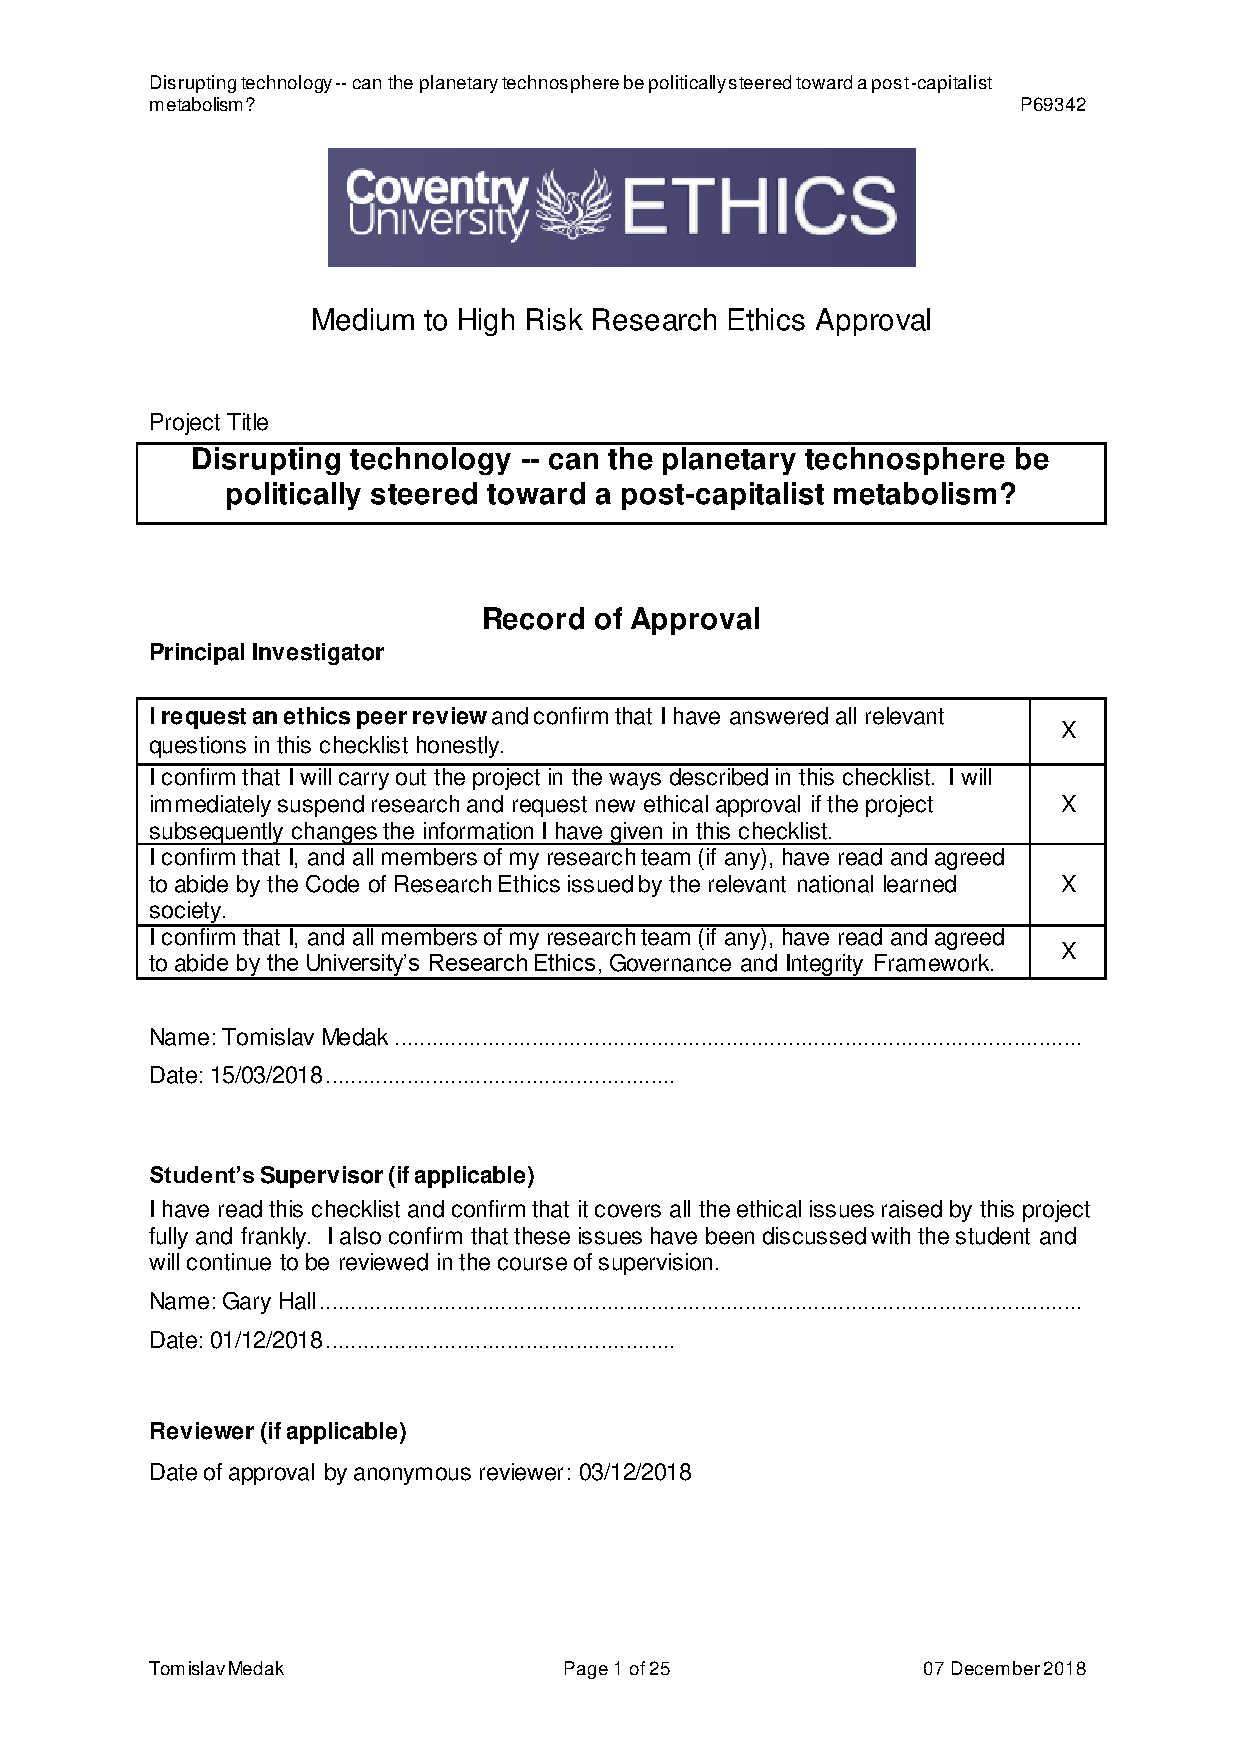
\includepdf[pages=-]{inserted-PDFs/ethics-approval.pdf}

\hypertarget{appendix-iii-permission-for-article-reuse}{%
\chapter{Appendix III: Permission for article reuse}\label{appendix-iii-permission-for-article-reuse}}

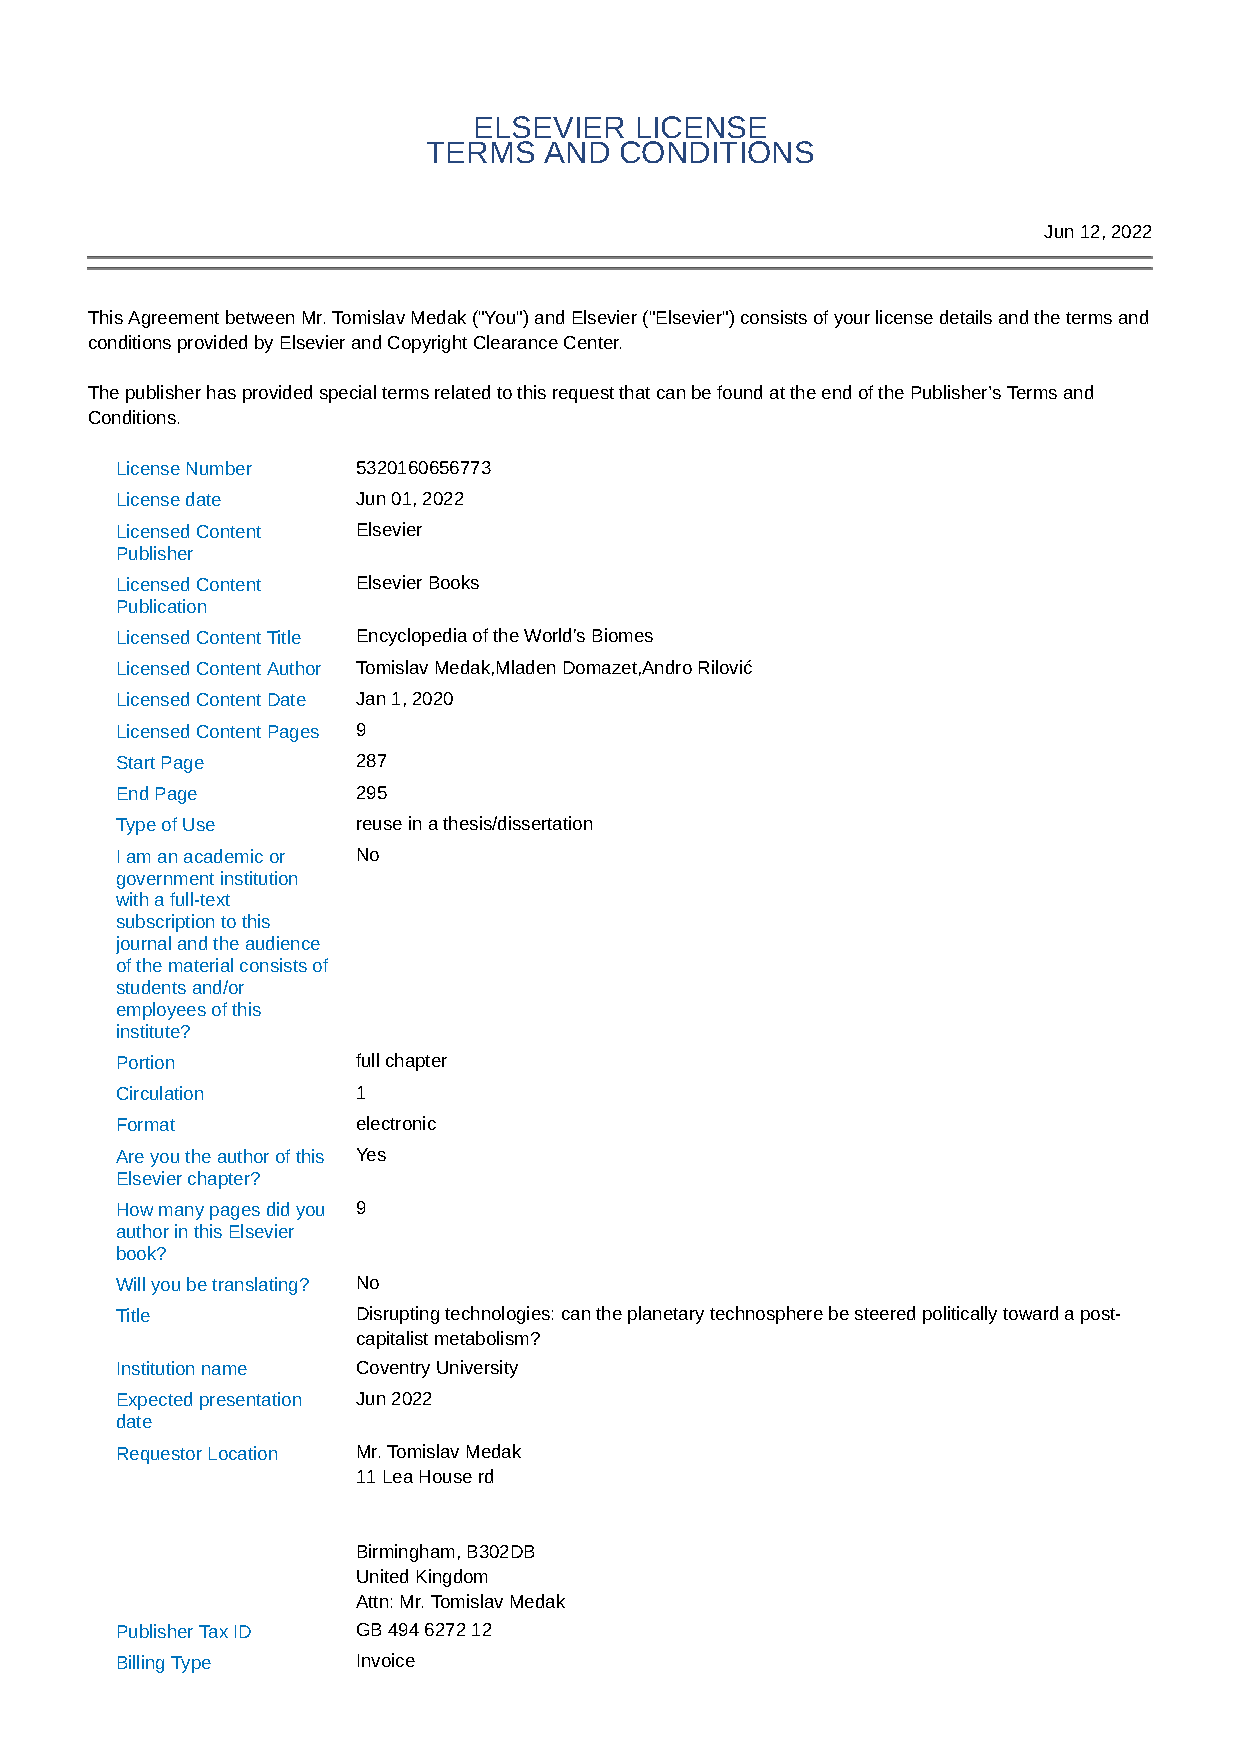
\includepdf[pages=-]{inserted-PDFs/permission-for-reuse.pdf}
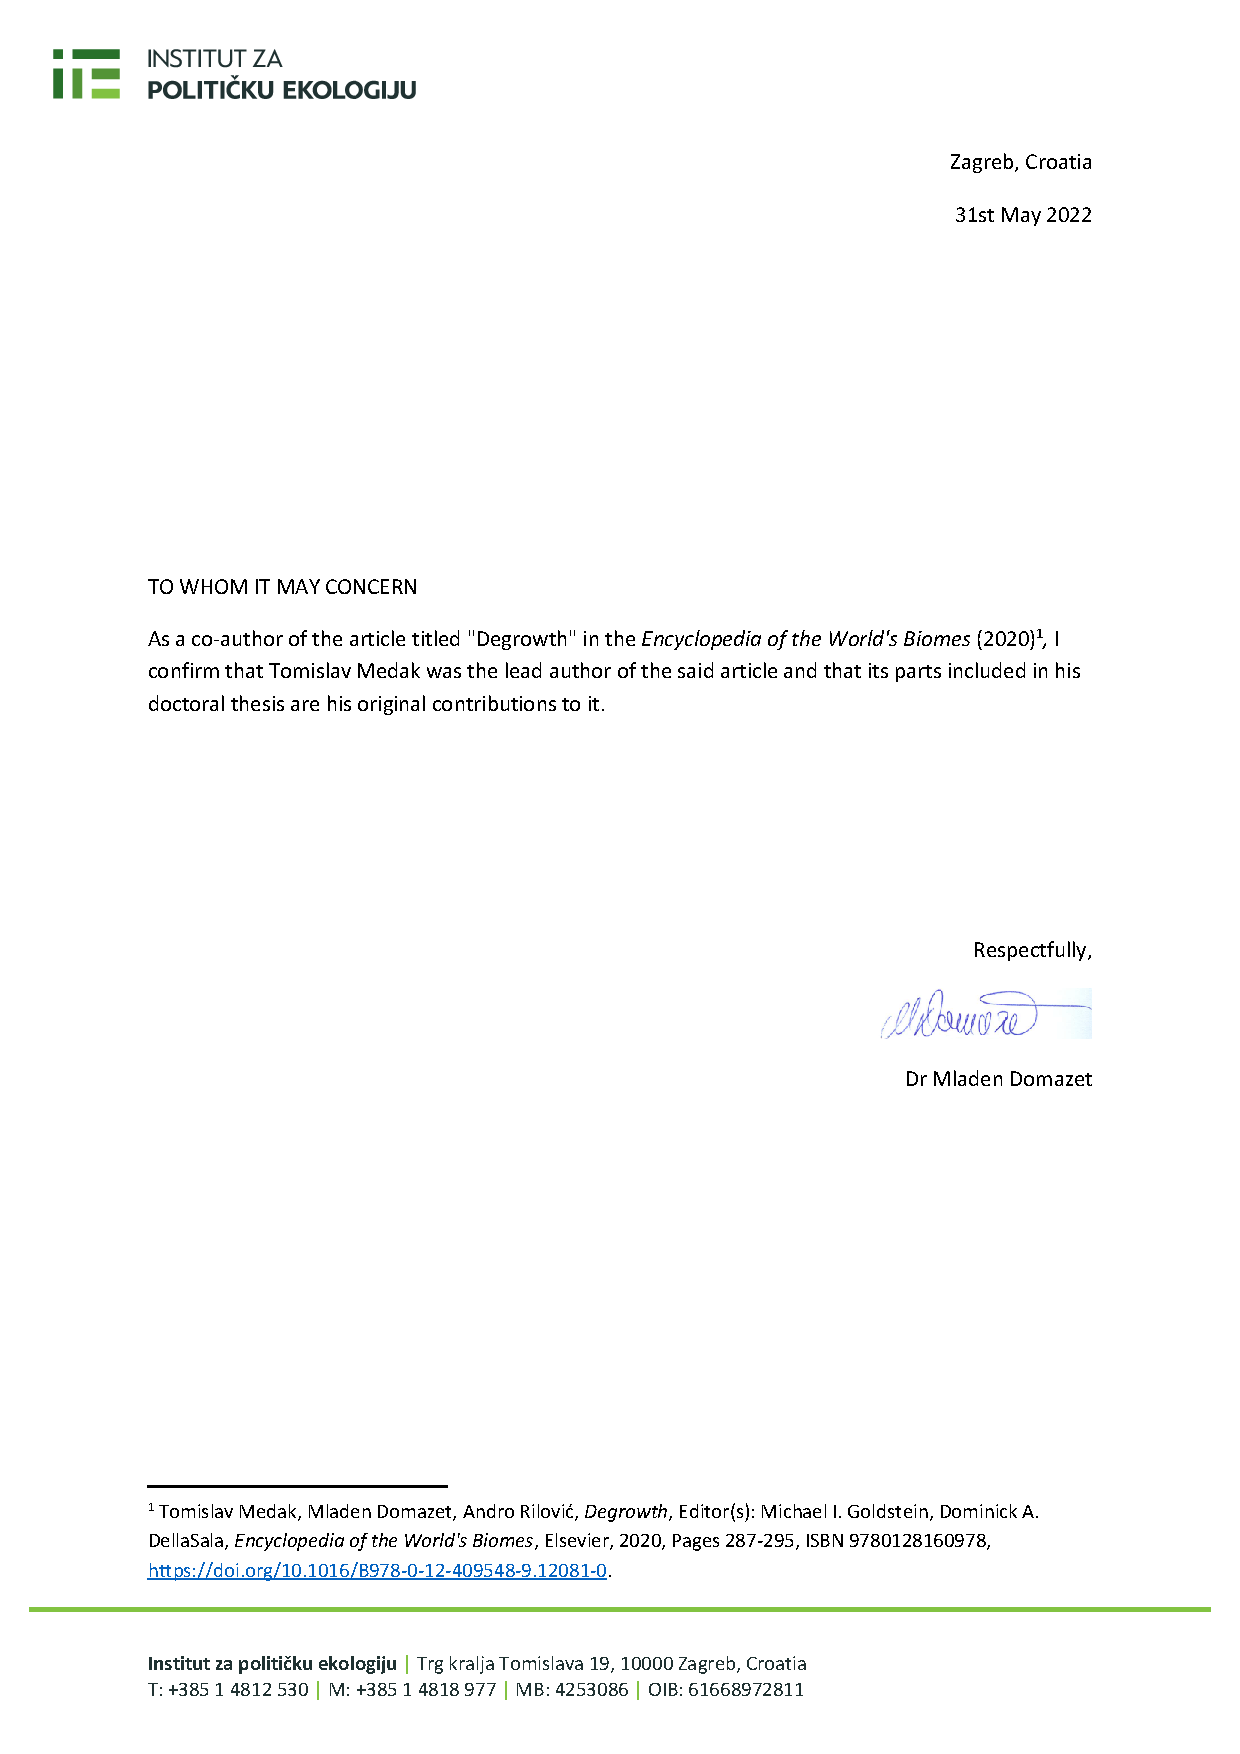
\includepdf[pages=-]{inserted-PDFs/Domazet-letter.pdf}

%%%%% REFERENCES


% set the section header to the references heading
\markboth{References}{}

\end{document}
